% Time-stamp: <2014-04-02 17:59 ycopin@lyonovae03.in2p3.fr>
% Auteurs (version LaTeX):
% Yannick Copin <ycopin@ipnl.in2p3.fr>
% Nicolas Chotard <nchotard@ipnl.in2p3.fr>
% Eric Chabanat <chabanat@ipnl.in2p3.fr>

% Version avec solutions:
%   pdflatex TD_astro_L2'
% Version sans solution:
%   pdflatex "\def\sanscorrige{}% Time-stamp: <2015-12-26 00:14 ycopin@lyonovae03.in2p3.fr>
% Auteurs (version LaTeX):
% Yannick Copin <ycopin@ipnl.in2p3.fr>
% Nicolas Chotard <nchotard@ipnl.in2p3.fr>
% Eric Chabanat <chabanat@ipnl.in2p3.fr>

% Version avec solutions:
%   pdflatex TD_astro_L2'
% Version sans solution:
%   pdflatex "\def\sanscorrige{}% Time-stamp: <2015-12-26 00:14 ycopin@lyonovae03.in2p3.fr>
% Auteurs (version LaTeX):
% Yannick Copin <ycopin@ipnl.in2p3.fr>
% Nicolas Chotard <nchotard@ipnl.in2p3.fr>
% Eric Chabanat <chabanat@ipnl.in2p3.fr>

% Version avec solutions:
%   pdflatex TD_astro_L2'
% Version sans solution:
%   pdflatex "\def\sanscorrige{}% Time-stamp: <2015-12-26 00:14 ycopin@lyonovae03.in2p3.fr>
% Auteurs (version LaTeX):
% Yannick Copin <ycopin@ipnl.in2p3.fr>
% Nicolas Chotard <nchotard@ipnl.in2p3.fr>
% Eric Chabanat <chabanat@ipnl.in2p3.fr>

% Version avec solutions:
%   pdflatex TD_astro_L2'
% Version sans solution:
%   pdflatex "\def\sanscorrige{}\input{TD_astro_L2}"

% À faire:
% * Exercice sur la méthode Baade-Wesselink
% (p.ex. http://arxiv.org/abs/1201.3478 et références,
% http://www.eso.org/public/news/eso0432/, 2004ApJ...603..285M)
% * Ajout de la théorie MOND dans l'exo sur la matière noire

\documentclass[a4paper,10pt]{report}

% PREAMBULE ==============================

\usepackage[utf8]{inputenc}
\usepackage{lmodern}
\usepackage[T1]{fontenc}

% Utilise CMbright (sans) pour les formules
\DeclareMathVersion{sans}
\SetSymbolFont{operators}{sans}{OT1}{cmbr}{m}{n}
\SetSymbolFont{letters}{sans}{OML}{cmbrm}{m}{it}
\SetSymbolFont{symbols}{sans}{OMS}{cmbrs}{m}{n}
\SetMathAlphabet{\mathit}{sans}{OT1}{cmbr}{m}{sl}
\SetMathAlphabet{\mathbf}{sans}{OT1}{cmbr}{bx}{n}
\SetMathAlphabet{\mathtt}{sans}{OT1}{cmtl}{m}{n}
\SetSymbolFont{largesymbols}{sans}{OMX}{iwona}{m}{n}

\usepackage[cm]{fullpage}
\usepackage[francais]{babel}
\DecimalMathComma

\usepackage{microtype}

\usepackage{amsmath, amssymb}
\usepackage{textcomp}
\usepackage{gensymb}

\usepackage{enumitem}           % enumerate[resume]

\usepackage[pdftex]{graphicx}
\graphicspath{{./Figures/}}

\usepackage{booktabs}

\usepackage[rightcaption]{sidecap}
\usepackage{caption}
\usepackage{subcaption}

\usepackage{siunitx}
\sisetup{%
  detect-all,
  free-standing-units,          % create standalone commands
  locale=FR, 
  inter-unit-product={\,},      % character between units
}
\DeclareSIUnit\Lsun{\ensuremath{\mathsf{\emph{L}}_{\odot}}}
\DeclareSIUnit\Rsun{\ensuremath{\mathsf{\emph{R}}_{\odot}}}
\DeclareSIUnit\Msun{\ensuremath{\mathsf{\emph{M}}_{\odot}}}
\DeclareSIUnit\pc{pc}           % parsec
\DeclareSIUnit\as{as}           % arcsec

\usepackage{hyperref}
\hypersetup{
  pdftitle   = {Astrophysique pour la licence, fascicule de TD},
  pdfauthor  = {Yannick Copin, pour l'équipe enseignante Astro-L2},
  pdfsubject = {Astrophysique pour la licence, Université de Lyon 1},
  unicode=true,              % non-Latin characters in Acrobat’s bookmarks
  linktoc=all,
  colorlinks=true,           % false: boxed links; true: colored links
  linkcolor=OliveGreen,      % color of internal links
  citecolor=OliveGreen,      % color of links to bibliography
  urlcolor=MidnightBlue,     % color of external links
  pdfencoding=auto,          % http://tex.stackexchange.com/questions/119079
  psdextra=true,
}
\usepackage{bookmark} % http://tex.stackexchange.com/questions/119079

% Make Adobe Reader use the RGB rendering model for pages with transparency
% http://tex.stackexchange.com/questions/16061/
\pdfpageattr{/Group << /S /Transparency /I true /CS /DeviceRGB>>}

% Définition de l'environnement 'Exercise'
\newcounter{noexo}
\setcounter{noexo}{0}
\newenvironment{Exercise}[1][]{%
  \refstepcounter{noexo}
  \medskip\noindent\textbf{Exercice~\thenoexo~:~#1}
  \medskip\par
  \addcontentsline{toc}{paragraph}{Exercice~\thenoexo~:~#1}
  \label{exo:\thenoexo}
}{}

% Définition de l'environnement 'Answer'
\usepackage[usenames, dvipsnames]{color}
\usepackage{comment}
\specialcomment{Answer}{%
  \begingroup
  \sffamily\color{CadetBlue}
  \mathversion{sans}
  %\medskip\noindent\textbf{Corrigé :~}
  \paragraph*{\textsf{Corrigé :}}
}{%
  \endgroup
}
% http://tex.stackexchange.com/questions/159820/comment-sty-and-utf8-encoding
\renewcommand\ThisComment[1]{%
  \immediate\write\CommentStream{\unexpanded{#1}}
}

% Inclusion ou non des corrigés
\ifdefined\sanscorrige
  \message{Fascicule sans solutions}%
  \excludecomment{Answer} % Remove answers
  \newcommand{\corrige}[1]{}
\else
  \message{Fascicule *AVEC* solutions}%
  \newcommand{\corrige}[1]{%
    \sffamily\color{CadetBlue}\mathversion{sans}#1}
\fi

% Définitions locales
%\newcommand{\e}[1]{\ensuremath{\times 10^{#1}}}
\newcommand{\e}[1]{\ensuremath{\times 10^{#1}}}
\renewcommand{\d}{\ensuremath{\mathrm{d}}}
\renewcommand{\deg}{\ensuremath{\degree}}
\renewcommand{\vec}[1]{\ensuremath{\boldsymbol{\mathbf{#1}}}}
%\renewcommand{\u}[1]{\ensuremath{\mathrm{#1}}} % Unités
\renewcommand{\u}[1]{\si{#1}} % Unités
\newcommand{\defeq}{\mathrel{\widehat=}}
\DeclareMathOperator{\grad}{\mathbf{grad}}

\newcommand{\farcm}{%
  \mbox{\ensuremath{.\mkern-4mu^\prime}}} % fractional arcminute symbol: 0.'0
\newcommand{\farcs}{%
  \mbox{\ensuremath{.\!\!^{\prime\prime}}}} % fractional arcsecond symbol: 0.''0
\newcommand{\fdg}{%
  \mbox{\ensuremath{.\!\!\degree}}}      % fractional degree symbol: 0.°0

\newcommand{\red}[1]{\textcolor{red}{#1}}
\newcommand{\note}[1]{\fcolorbox{red}{yellow}{\color{black} #1}}

% PAGE DE TITRE ET PREAMBULE ==============================

\makeatletter
\def\thickhrulefill{\leavevmode \leaders \hrule height 1pt\hfill \kern \z@}
\renewcommand{\maketitle}{\begin{titlepage}%
    \let\footnotesize\small
    \let\footnoterule\relax
    \parindent \z@
    \reset@font
    \null
    \begin{center}
      \huge \bfseries \@title
      \ifdefined\sanscorrige
      \else
      \\\textcolor{red}{avec solutions}
      \fi
    \end{center}
    \hrule height 1pt
    \begin{flushright}
      Université Claude Bernard Lyon1 \\
    \end{flushright}
    \vfil
    \vfil
    \begin{figure}[htp]
      \centering
      \includegraphics[width=0.8\textwidth]{flammarion}
      \caption{La gravure sur bois dite «~de Flammarion~».}
    \end{figure}
    \begin{center}
    \vfil
      {\Large \@author} \\[1em]
      {\large \@date}
    \end{center}
  \end{titlepage}%
  \setcounter{footnote}{0}%
}
\makeatother

\title{Fascicule de TD}
\date{\small Version du \today}
\author{Astrophysique pour la licence\\[\medskipamount]Université Lyon 1}

\begin{document}

\maketitle

% 2: Down to subsection (no exercices)
% 4: Down to paragraph (exercices)
\setcounter{tocdepth}{4}
\tableofcontents

\newpage

% EXERCICES ET SOLUTIONS ==============================

\chapter{Vie des étoiles}

\section{La lumière des étoiles}

\subsection{Photosphère et température effective}

\begin{Exercise}[Luminosité du Soleil]
  Calculer la luminosité du Soleil à partir de sa température
  effective $T_\odot \approx \SI{5770}{K}$ et de son rayon
  $\Rsun \approx \SI{6,96e8}{m}$.
\end{Exercise}

\begin{Answer}
  Dans l'hypothèse du corps noir, la luminosité est reliée à la
  température et au rayon par $\Lsun = 4 \pi \Rsun^2 \sigma
  T_{\odot}^{4}$ avec la constante de Stefan $\sigma =
  \SI{5,67e-8}{W.m^{-2}.K^{{-4}}}$, soit $\Lsun \approx
  \SI{3,83e26}{W}$.
\end{Answer}


\begin{Exercise}[Rayon des étoiles]
  Déterminer le rayon (en unité solaire), la longueur d'onde de Wien
  et la couleur «~visible~» des étoiles suivantes :
  \begin{enumerate}
  \item Naine blanche : $L = \SI{e-2}{\Lsun}$, $T_{e} = \SI{20000}{K}$
  \item Géante rouge : $L = \SI{e2}{\Lsun}$, $T_{e} = \SI{4200}{K}$
  \item Supergéante : $L = \SI{e5}{\Lsun}$, $T_{e} = \SI{6000}{K}$
  \end{enumerate}
  Rappel de la loi de Wien : $\lambda_{\max} T = \SI{2898}{\micro\meter\K}$.
\end{Exercise}

\begin{Answer}
  \begin{center}
    \begin{tabular}{lccccl}
      \toprule
      Type stellaire & $L$~[\Lsun] & $T_{e}$~[K] &
      $R$~[\Rsun] & $\lambda_{\max}$ [nm] & Couleur \\
      \midrule
      Naine blanche & $10^{-2}$ & 20000  & 0,008 & 145 & Blanc \\
      Géante rouge  & $10^{2}$  & 4200  & 18,8   & 690 & Rouge \\
      Supergéante   & $10^{5}$  & 6000  & 291,7  & 483 & Bleu \\
      \bottomrule
    \end{tabular}
  \end{center}
\end{Answer}


\begin{Exercise}[Équilibre radiatif de la Terre]
  %\textbf{Rappel :} Le \emph{flux} est une puissance par unité de
  %surface (unités~SI : \u{J~s^{-1}~m^{-2}}).

  Soit $L$ la puissance lumineuse du Soleil, $R$ le rayon de la Terre,
  $D$ la distance Terre-Soleil et $T_{e}$ la température effective à
  la surface de la Terre :
  \begin{enumerate}
  \item Écrire la relation entre $L$ et $F(D)$, le flux lumineux à une
    distance $D$ du Soleil. En déduire la puissance lumineuse totale
    $P_{r}$ reçue par la Terre.
    % (on suppose que la terre est vue du Soleil comme un disque de
    % rayon $R$)
  \item Utiliser la loi de Stefan et expliciter le flux lumineux
    $F_e$, puis la puissance totale $P_e$, rayonnés par la Terre.
  \item Écrire l'égalité des puissance reçue et rayonnée à la surface
    de la Terre, en déduire l'expression de la température $T_{e}$ en
    fonction des données du problème.
  \item Application numérique, sachant que $L = \SI{3,85e26}{W}$, $R =
    \SI{6400}{km}$, $D = \SI{1,500e11}{m}$, $\sigma =
    \SI{5,67e-8}{W.m^{-2}.K^{-4}}$.
  \item Commenter sur la validité et les limites de ce modèle.
   \end{enumerate}
\end{Exercise}

\begin{Answer}
  \begin{enumerate}
  \item $F(D) = L / 4\pi D^2$, $P_{r} = L R^2/(4 D^2)$
  \item $F_e = \sigma T_{e}^4$ et $P_e = 4\pi R^2 \sigma T_{e}^4$
  \item $P_e = P_r$ d'où $T_{e} = \left( L / (16\pi D^2\sigma)
    \right)^{1/4} = 278$~K.
  \end{enumerate}
\end{Answer}


\subsection{Système de magnitudes}

\begin{Exercise}[Système binaire]
  Les deux composantes de l'étoile $\alpha$ du Centaure située à
  1,32~pc de distance ont des magnitudes visuelles (magnitude
  apparente dans la bande $V$) de 0,30 et 1,70. On demande :
  \begin{enumerate}
  \item Le rapport des flux des deux étoiles dans la bande $V$.
  \item La magnitude visuelle globale du système.
  \item La correction qu'il faut apporter aux magnitudes apparentes de
    ce système pour obtenir les magnitudes absolues.
  \end{enumerate}
\end{Exercise}

\begin{Answer}
  On rappelle que la magnitude apparente $m$ est liée au flux $f$ par
  $m = -2,5 \log_{10}(f / f_{0})$.
  \begin{enumerate}
  \item Le rapport des flux des deux composantes de $\alpha$~Cen
    dépend de la différence de magnitudes et vaut :
    $$
    f_2 / f_1 = 10^{(m_{1} - m_{2})/2,5} = 0,28
    $$
  \item La magnitude apparente visuelle globale du système
    $m_{\Sigma}$ se calcule à partir du flux total $f_{\Sigma} = f_{1}
    + f_{2}$ (les puissances émises par les deux composantes
    s'ajoutent) :
    $$
    m_{\Sigma} = -2,5 \log(f_{\Sigma} / f_{0}) = 
    %-2,5 \log(f_{1}/f_{0} + f_{2}/f_{0}) =
    -2,5 \log(10^{-m_{1}/2,5} + 10^{-m_{2}/2,5}) = 0,04
    $$
  \item La différence entre magnitudes apparente $m$ et absolue $M$
    correspond au module de distance $\mu$ du système :
    $$
    \mu = m - M = 5 \log(D/\SI{10}{\pc}) = -4,4
    $$
  \end{enumerate}
\end{Answer}


\section{Classification spectrale}

\subsection{Mesures des distances}

\subsubsection{Parallaxe trigonométrique}

\begin{Exercise}[Incertitude]
  Relier l'incertitude sur la distance $\Delta D$ à celle sur la
  parallaxe $\Delta p$.
\end{Exercise}

\begin{Answer}
  Il existe deux méthodes pour trouver le résultat demandé :
  \begin{itemize}
  \item En différenciant l'équation $D = 1/p$, on obtient $\d D =
    -(1/p^2)\d p$, d'où l'incertitude en prenant la valeur absolue :
    $$
    \Delta D = \frac{1}{p^2}\Delta p = \frac{D}{p}\Delta p
    \quad\text{soit finalement}\quad 
    \Delta D/D = \Delta p/p.
    $$

  \item On peut également prendre le logarithme de l'équation $D =
    1/p$, ce qui donne $\ln~D = -\ln~p$, puis on différencie :
    $\d\ln~D = -\d\ln~p$, soit $\d D/D = -\d p/p$. En prenant la
    valeur absolue, on retrouve le résultat précédent.
  \end{itemize}
\end{Answer}

\begin{Exercise}[Astrométrie spatiale]
  Considérons les deux missions d'astrométrie spatiale : Hipparcos
  (1989), avec une incertitude absolue sur la mesure de la parallaxe
  typique de $\Delta p = 2$~mas, et Gaia (2013), avec $\Delta p =
  7$~$\mu$as. Quelles sont les précisions obtenues à une distance de
  100~pc ? de 1000~pc ?  À quelle distance aura-t-on une erreur de
  100\% ?
\end{Exercise}

\begin{Answer}
  Les étoiles situées à $D = 100$~pc ont une parallaxe $p = 1/100 =
  0\farcs 01 = 10$~mas. La précision obtenue sera de
  \begin{align*}
    \text{Hipparcos:}\quad \frac{\Delta D}{D} &= \frac{\Delta p}{p} =
    \frac{2\e{-3}}{10^{-2}} = 2\e{-1} = 20 \% \\
    \text{Gaia:}\quad \frac{\Delta D}{D} &= \frac{\Delta p}{p} = 
    \frac{7\e{-6}}{10^{-2}} = 7\e{-4} = 0,07 \%
  \end{align*}
  Pour des étoiles à $D=1000$~pc, $p=1$~mas, et les précisions
  deviennent 10 fois moins bonnes : 200\% avec Hipparcos et 0,7\% avec
  Gaia.

  On aura une erreur de 100\% quand $\Delta D = D$, soit $\delta p =
  p$. La distance correspondante s'obtient donc par
  \begin{align*}
    \text{Hipparcos:}\quad D_{\max} &= 1/p = 1/2\e{-3} = \SI{500}{\pc} \\
    \qquad\text{Gaia:}\quad D_{\max} &= 1/p = 1/7\e{-6} = \SI{143}{\kilo\pc}
  \end{align*}
\end{Answer}

\begin{Exercise}[Parallaxe et magnitude absolue]
  Le tableau suivant donne la magnitude apparente $m_V$ et la
  parallaxe $p$ de trois étoiles. Calculer leur distance $D$ avec son
  incertitude, l'erreur relative sur la distance $\Delta D / D$ et
  leur magnitude absolue $M_V$.
  \begin{center}
    \begin{tabular}{lccc}
      \toprule
      & $\alpha$ CMa (Sirius) & $\alpha$ Tau (Aldebaran) & $\alpha$ Ori
      (Bételgeuse) \\
      \cmidrule(r){2-4}
      $m_V$ & $-1,47$ & $0,85$ & $0,58$ \\
      $p$ (mas) & $379,2 \pm 1,6$ & $50,1 \pm 1,0$ & $7,6 \pm 1,6$ \\
      \bottomrule
    \end{tabular}
  \end{center}
\end{Exercise}

\begin{Answer}
  \begin{center}
    \begin{tabular}{lccc}
      \toprule
      & $\alpha$ CMa & $\alpha$ Tau & $\alpha$ Ori \\
      \cmidrule(r){2-4}
      $D$ (pc) &
      $2,637 \pm 0,012$ & $19,96 \pm 0,40$ & $132 \pm 28$ \\
      $\Delta D / D$ & 0,4\% & 2\% & 21\% \\
      $M_V$ & $1,42$  & $-0,65$ & $-4,99$ \\
      \bottomrule
    \end{tabular}
  \end{center}
  Étant donné la forme de la relation donnant la distance $D$ à partir
  de la parallaxe $p$, leurs incertitudes relatives sont égales, ce
  qui permet d'avoir immédiatement $\Delta D / D$. Ces résultats
  illustrent bien la diminution de la précision lorsque la distance
  augmente.  La magnitude absolue s'obtient par la relation $M_V = m_V
  - 5~\log(D/\SI{10}{\pc})$.
\end{Answer}


\begin{Exercise}[Méthode du point convergent]
  On veut déterminer la distance de l'amas des Pléiades par la méthode
  du point convergent.
  \begin{itemize}
  \item L'étude des trajectoires des étoiles de l'amas sur plusieurs
    années a permis de situer le point convergent à $\theta = 67,9 \pm
    0,6\deg$ de la direction de l'amas.
  \item L'observation du spectre de l'étoile Alcyone, faisant partie
    de cet amas, a permis de mesurer sa vitesse radiale $v_r = 10,1
    \pm \SI{0,3}{km.s^{-1}}$.
  \item Le mouvement propre apparent de cette même étoile vaut $\mu =
    47,3 \pm \SI{0,8}{\milli\as~an^{-1}}$.
  \end{itemize}
  Déterminer la distance de l'amas.
\end{Exercise}

\begin{Answer}
  Dans la formule donnant la distance de l'amas, il faut bien faire
  attention à exprimer l'angle $\mu$ en radians et à utiliser les
  mêmes unités de distance et de temps pour les autres grandeurs.
  \begin{itemize}
  \item $\mu = 47,3 \pm 0,8~\u{mas~an^{-1}} = 
    (2,29 \pm 0,04) \e{-7}~\u{rad~an^{-1}}$
  \item $v_r = 10,1 \pm 0,3~\u{km~s^{-1}} = 
    (1,02 \pm 0,03) \e{-5}~\u{pc~an^{-1}}$
  \item $\theta = 67,9 \pm 0,6\deg = 1,19 \pm 0,01$~rad, et donc $\tan
    \theta= 2,50 \pm 0,07$.
  \end{itemize}
  Finalement, $D = v_{r}\tan\theta/\mu = 111 \pm 8$~pc. L'erreur est
  obtenue via $\d D = (\tan\theta/\mu)\d v_{r} +
  (v_{r}/\mu)(1-\tan^{2}\theta)\d\theta -
  (v_{r}\tan\theta/\mu^{2})\d\mu$.
\end{Answer}

\subsection{Classification stellaire}

\begin{SCfigure}[0.5]
  \centering
  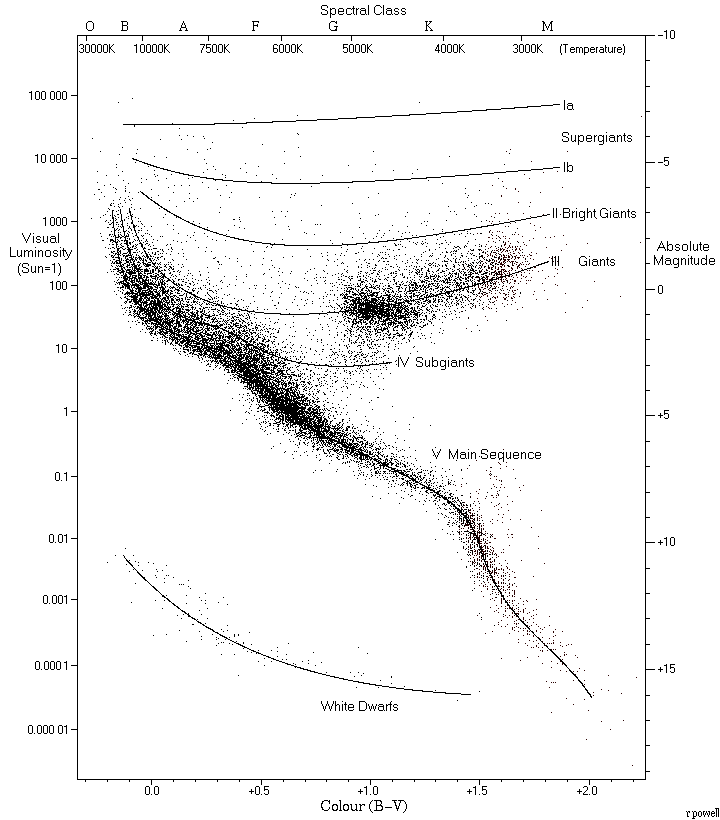
\includegraphics[width=0.5\textwidth]{hr}
  \caption{Diagramme de Hertzsprung-Russell des 22000 étoiles du
    catalogue Hipparcos et de 1000 étoiles faiblement lumineuses du
    catalogue Gliese des étoiles proches.}
  \label{hr}
\end{SCfigure}

\begin{Exercise}[Types spectraux]
  Donner approximativement le type spectral des étoiles dont le flux
  est maximal aux longueurs d'onde suivantes : 300~nm, 500~nm, et
  1,2~$\mu$m.  Peut-on déterminer la classe de luminosité ?

  Rappel de la loi de Wien : $\lambda_{\max} T = 2898$~\u{\micro m~K}.
\end{Exercise}

\begin{Answer}
  La loi de Wien permet de déterminer la température effective de
  chaque étoile, et ainsi d'en déduire une valeur approximative du
  type spectral. Ici seulement la première lettre est accessible, la
  détermination du chiffre suivant nécessiterait un tableau plus
  précis donnant les correspondances entre les sous-types et la
  température effective.
  \begin{center}
    \begin{tabular}{ccc}
      \toprule
      $\lambda_{\max}$ & $T_{\mathrm{eff}}(K)$ & Type spectral \\
      \midrule
      300 nm & 9660 & A  \\
      500 nm & 5796 & G \\
      1,2 $\mu$m & 2415 & M \\
      \bottomrule
    \end{tabular}
  \end{center}
  On ne peut pas déterminer la classe de luminosité grâce à la
  longueur d'onde du maximum du flux. Pour ceci, il faudrait connaître
  soit la luminosité de l'étoile, soit sa gravité de surface, soit son
  rayon.
\end{Answer}

\begin{Exercise}[Diagramme HR]
  Classer par ordre de température effective croissante, puis de rayon
  croissant, et enfin de luminosité croissante les étoiles de types
  spectraux suivants : M5III, O2V, K7I, A0VII.
\end{Exercise}

\begin{Answer}
  La séquence OBAFGKM décrit les types spectraux dans le sens des
  $T_{\mathrm{eff}}$ décroissantes, on aura donc dans le sens des
  $T_{\mathrm{eff}}$ croissantes : M5III, K7I, A0VII, et O2V.

  La classe de luminosité définit des groupes d'étoiles de rayon
  différent, on aura donc dans l'ordre croissant : A0VII, O2V, M5III,
  et K7I.

  Enfin, l'examen du diagramme HR montre qu'une étoile chaude de la
  séquence principale peut être plus lumineuse qu'une sous-géante
  froide, et on aura dans le sens des luminosités croissantes : A0VII,
  M5III, O2V, et K7I.

  Ceci montre que le terme «~classe de luminosité~» peut être source
  d'erreur.
\end{Answer}

\subsection{Mesure des rayons}

\begin{Exercise}[Interférométrie]
  Le tableau suivant donne le diamètre apparent $\theta_*$ des étoiles
  de l'exercice~\ref{exo:10}, mesuré par interférométrie. Calculer
  leur rayon $R$ (on rappelle les distances déterminées dans un
  exercice précédent) et, à l'aide de ce résultat, attribuer à chaque
  étoile sa classe de luminosité parmi les suivantes : I, III, V.
  \begin{center}
    \begin{tabular}{lccc}
      \toprule
      & $\alpha$ CMa & $\alpha$ Tau & $\alpha$ Ori \\
      \cmidrule(r){2-4}
      $\theta_*$ [mas] & 5,89 & 24 & 67 \\
      $d$ [pc] & 2,64  & 20  & 130 \\
      \bottomrule
    \end{tabular}
  \end{center}
\end{Exercise}

\begin{Answer}
  Pour Sirius, le rayon vaut $R[\u{UA}] = d[\u{pc}] \times
  \theta_*[''] / 2$ soit $R = \SI{7,8e-3}{ua} = \SI{1,67}{\Rsun}$.
  Le tableau suivant donne les résultats pour les 3 étoiles :
  \begin{center}
    \begin{tabular}{lccc}
      \toprule
      & $\alpha$ CMa & $\alpha$ Tau & $\alpha$ Ori \\
      \cmidrule(r){2-4}
      $R/\Rsun$ & 1,67 & 52 & 936 \\
      Classe de luminosité & V & III & I \\
      Type spectral & A1V & K5III & M2I \\
      \bottomrule
    \end{tabular}
  \end{center}
  Dans cet exemple, il est possible d'attribuer à chaque étoile sa
  classe de luminosité en utilisant le lien qui existe avec le rayon
  stellaire. Le type spectral complet est donné pour information.
\end{Answer}

\subsection{Mesure de masse (étoiles doubles)}

\begin{Exercise}[Système binaire]
  On observe une étoile double visuelle dont le plan de l'orbite est
  perpendiculaire à la ligne de visée.
  \begin{itemize}
  \item La parallaxe de ce système est de 100~mas.
  \item La plus grande séparation angulaire entre les deux composantes
    est de $5''$, et la plus petite de $1''$.
  \item La période de révolution est de 30~ans.
  % \item L'étoile primaire se trouve au foyer de l'orbite observée, car
  %   il n'y a pas d'effet de projection.
  \item Le compagnon est toujours observé à une distance du centre de
    gravité 5~fois plus grande que celle de l'étoile primaire.
  \end{itemize}
  Déterminer la masse de chaque composante.
\end{Exercise}

\begin{Answer}
  Les paramètres observés permettent de remonter aux données suivantes
  pour le système :
  \begin{itemize}
  \item La distance est $D[\u{pc}] = 1/p[''] = 10$~pc.
  \item La dimension angulaire du grand axe de l'orbite relative est
    de $5'' + 1'' = 6''$. Le demi-grand axe apparent est donc $\theta
    = 3'' = 1,45\e{-5}$~rad.
  \item Le demi-grand axe de l'orbite relative est donné par
    $a[\u{UA}] = \theta[''] D[\u{pc}]$ soit $a = 30\;\u{UA} =
    4,49\e{12}\;\u{m}$.
  \item La 3ème loi de Kepler (en unités réduites) donne la somme des
    masses : $M_{1} + M_{2} = 30\;\Msun = 5,97\e{31}$~kg.
  \item Les distances des étoiles $E_1$ et $E_2$ au centre de gravité
    $G$ vérifient $M_1 \times GE_1 = M_2 \times GE_2$. Le rapport des
    masses vaut donc $M_1 / M_2 = GE_2 / GE_1 = 5$.
  \item Finalement : $M_1 = 25\;\Msun$ et $M_2 = 5\;\Msun$
  \end{itemize}
\end{Answer}


\begin{Exercise}[Le paradoxe d'Algol]
  Le tableau suivant rappelle les caractéristiques du système binaire
  à éclipse d'Algol ($\beta$~Per):
  \begin{center}
    \begin{tabular}{lcc}
      \toprule
      $p$ (mas) & \multicolumn{2}{c}{35,14 $\pm$ 0,90} \\
      $T$ (jours) & \multicolumn{2}{c}{2,8674} \\
      $\theta_{\mathrm{rel}}$ [mas] & \multicolumn{2}{c}{2,283} \\
      \midrule
      Composantes & $A$ & $B$ \\
      \cmidrule(r){2-3}
      Type spectral & B8V & K2IV \\
      $R/\Rsun$ & 2,74 & 3,60 \\
      $\theta_{\mathrm{abs}}$ (mas) & & 1,872 \\
      \bottomrule
    \end{tabular}
  \end{center}
  On supposera l'orbite circulaire, ainsi le demi-grand axe de
  l'ellipse projetée est égal au rayon de l'orbite.

  \begin{enumerate}
  \item Quelle est la distance (et son erreur) de ce système ?
  \item Quelle est la séparation des deux étoiles ? Comparez-la à
    leurs rayons.
  \item Quelle est la masse de chacune des étoiles ? Compte-tenu des
    types spectraux, décrire le \emph{paradoxe d'Algol} et suggérer
    une solution.
  \end{enumerate}
\end{Exercise}

\begin{Answer}
  \begin{itemize}
  \item Distance : $D [\u{pc}] = 1/p[''] = 28,46 \pm 0,73$~pc.
  \item Le demi-grand axe de l'orbite relative est donné par $a
    [\u{UA}] = \theta [''] D [\u{pc}]$ soit $a = 0,065~\u{UA} =
    9,77\e{9}~\u{m} = 13,96\;\Rsun = 2,2 (R_{A}+R_{B})$.
  \item La 3ème loi de Kepler donne la somme des masses réduites
    ($\tilde{M} = M/\Msun$) : $\tilde{M}_A + \tilde{M}_B =
    \tilde{a}^3/\tilde{T}^2 = 4,46$ (avec $\tilde{a} = a[\u{UA}]$ et
    $\tilde{T} = T[\u{an}]$)
  \item Le rapport des demi-grands axes apparents de l'orbite relative
    $\theta$ et de l'orbite absolue de l'étoile secondaire $\theta_B$
    donne le rapport des masses : $\theta_B / \theta = a_B / a = M_A /
    (M_A + M_B) = 0,82$
  \item On obtient finalement les masses $M_A = 3,65\;\Msun$ et $M_B =
    0,80\;\Msun$.
  \end{itemize}
  Le tableau suivant récapitule les données physiques du système :
  \begin{center}
    \begin{tabular}{lcc}
      \toprule
      $D$ (pc) & \multicolumn{2}{c}{28,46 $\pm$ 0,73} \\
      $a/\Rsun$ & \multicolumn{2}{c}{13,96} \\
      \midrule
      & $A$ & $B$ \\
      \cmidrule(r){2-3}
      $M/\Msun$ & 3,65 & 0,80 \\
      \bottomrule
    \end{tabular}
  \end{center}
  On remarque que l'étoile la plus évoluée, $B$ ($B$ est une
  sous-géante rouge, tandis que $A$ est une étoile de la séquence
  principale) est pourtant la moins massive, ce qui est
  contre-intuitif en terme d'évolution stellaire (les étoiles les plus
  massives évoluent plus rapidement). On peut invoquer des transferts
  de masse au sein de ce système très serré pour expliquer ce
  paradoxe.
\end{Answer}

\section{Les systèmes planétaires}

\subsection{Les lois de Kepler}

\begin{Exercise}[Invariant de Runge-Lenz]
  On considère une particule $P$ de masse $m$, animée d'un mouvement
  non relativiste par rapport à un repère d'origine $O$. Ce mouvement
  est dû à un champ de forces $\vec{F} (\vec{r}) = - \grad U (r) $
  dérivant d'un potentiel central $U (r)$, où $\vec{r} = \vec{OP}$.

  À l'instant $t$ on note respectivement $\vec{v} (t)$, $\vec{a} (t)$
  et $\vec{p} (t)$ la vitesse, l'accélération et la quantité de
  mouvement de la particule $P$.

  \begin{enumerate}
  \item Montrer que la force $\vec{F}$ est radiale.
  \item Montrer que le vecteur moment cinétique $\vec{L} = \vec{r}
    \wedge \vec{p}$ est conservé au cours du mouvement.  En déduire
    que la trajectoire de $P$ est située dans un plan $\Pi$ que l'on
    caractérisera.
  \item Montrer que l'énergie mécanique $E= \dfrac{1}{2} m v^2 + U$
    est une constante du mouvement.
  \item Calculer $L$ à l'aide des coordonnées polaires $(r,\theta)$
    dans le plan $\Pi$ et en déduire la loi des aires.
  \end{enumerate}
  Dans toute la suite du problème, le potentiel est de la forme :
  $$
  U (r) = - \frac{k}{r} \qquad \text{avec} \qquad k>0
  $$
  On définit le \emph{vecteur de Runge-Lenz} :
  $$
  \vec{A} = \frac{1}{k} \, \vec{v} \wedge \vec{L} - \frac{\vec{r}}{r}
  $$
  \begin{enumerate}[resume]
  \item Montrer que le vecteur $\vec{A}$ est constant dans le temps,
    et qu'il appartient au plan $\Pi$.
  \item Montrer que :
    $$
    A^2 = 1+2 \, \frac{L^2 \, E}{mk^2}
    $$
    (On pourra utiliser les coordonnées polaires : en particulier $
    \vec{v} = v_r \, \vec{e}_r + v_{\theta} \, \vec{e}_{\theta} $).
    En déduire, lorsque $L$ est fixé, une borne inférieure pour
    l'énergie $E$.  Montrer que pour un mouvement circulaire, $E$ est
    égal à la borne inférieure.
  \item Calculer le produit scalaire $\vec{A}.\vec{r}$ en fonction de
    $L$, $m$, $k$ et $r$.  Établir alors l'équation polaire de la
    trajectoire sous la forme :
    $$
    r (\theta) = \frac{p}{1+e \, \cos \theta}
    $$
    \emph{Indication : on définira l'angle $\theta$ à partir de l'axe
      polaire dirigé selon le vecteur $\vec{A}$.}

    Vérifier que : $e =\|\vec{A}\|$ et exprimer $p$ en fonction de
    $L$, $m$ et $k$.
  \item Discuter la nature de la trajectoire suivant la valeur de $E$.
  \end{enumerate}
  Dans la suite du problème on se restreint au cas des \emph{états
    liés} : $E<0$. La trajectoire est alors une ellipse.
  \begin{enumerate}[resume]
  \item Déterminer son demi-grand axe $a$ et son demi-petit axe $b$ en
    fonction de $m$, $k$, $L$ et $E$.
  \item Quelle est la valeur maximale $L_0$ de $L$, l'énergie $E$
    étant fixée ?
  \item Quelle est la trajectoire pour $L=0$, et pour $L=L_0$ ?
  \item Calculer la période du mouvement en fonction de $m$, $k$ et
    $a$.
  \end{enumerate}
\end{Exercise}

\begin{Answer}
  \begin{enumerate}
  \item $\vec{F} = - (\partial U/\partial r) \vec{e}_{r}$.
  \item $\vec{L} = mr^{2}\dot{\theta}\vec{e}_{z}$ et $\d S/\d t = C/2$
    avec $C \equiv r^{2}\dot{\theta}$.
  \item $r = \dfrac{L^{2}/km}{1+A\cos\theta} = p/(1+e\cos\theta)$
  \item
    \begin{itemize}
    \item Si $E < 0$: système lié, $e < 1$, trajectoire elliptique;
    \item si $E = 0$: $e = 1$, trajectoire parabolique;
    \item si $E > 0$: système ouvert, $e > 1$, trajectoire
      hyperbolique.
    \end{itemize}
  \end{enumerate}
\end{Answer}

\begin{Exercise}[Orbite de Pluton]
  L'orbite de Pluton est très excentrique ($e=0,248$). Son demi-grand
  axe vaut 39,43~unités astronomiques (L'unité astronomique est
  définie comme le demi grand axe de l'orbite de la Terre). Montrer
  que Pluton peut être plus proche du Soleil que Neptune dont le
  demi-grand axe de l'orbite vaut 30,06~UA et l'excentricité~0,009.
\end{Exercise}

\begin{Answer}
  \begin{center}
    \begin{tabular}{lccc}
      \toprule
      & & Neptune & Pluton \\
      \cmidrule(r){2-4}
      Demi-grand axe [UA] & $a$ & 30,06 & 39,43 \\
      Excentricité & $e$ & 0,009 & 0,248 \\
      Périhélie [UA] & $d=a(1-e)$ & 29,79 & 29,65 \\
      Aphélie [UA] & $D=a(1+e)$ & 30,33 & 49,21 \\
      \bottomrule
    \end{tabular}
  \end{center}
  Du fait de la très grande excentricité de son orbite, Pluton, à son
  périhélie, est plus proche que Neptune du Soleil: $d_{P} < d_{N}$.
\end{Answer}

\begin{Exercise}[Vitesses périhélique et aphélique]
  Montrer que la vitesse angulaire d'un objet décrivant une orbite
  elliptique autour du Soleil augmente lorsqu'il s'en
  rapproche. Montrer que le rapport des vitesses au périhélie (point
  le plus proche du Soleil) et à l'aphélie (point le plus éloigné du
  Soleil) ne dépend que de l'excentricité de l'orbite.  Calculer ce
  rapport pour la Terre dont l'excentricité de l'orbite vaut 0,0167,
  puis pour la comète de Halley dont l'excentricité de l'orbite vaut
  0,97.
\end{Exercise}

\begin{Answer}
  \begin{enumerate}
  \item On a vu que $r^2\dot{\theta}$ est une constante. On a donc
    $\dot{\theta}=C/r^2$ et la vitesse angulaire augmente lorsque $r$
    diminue.

  \item L'expression de la vitesse est : $\vec{v} = \dot{r}\vec{i} +
    r\dot{\theta}\vec{j}$

    Le périhélie et l'aphélie correspondent à des extremum sur la
    trajectoire, c'est à dire que $\d r/\d\theta =0$ et donc,
    puisque $\dot{r} = \dot{\theta}~\d r/\d\theta$,
    $\dot{r}=0$. La vitesse s'écrit donc bien $v = r\dot{\theta}$

  \item Puisque $r^2\dot{\theta}=C$ et que $v = r\dot{\theta}$, on a
    $v = C/r$. En reprenant les résultats vus précédemment sur les
    ellipses, on trouve $r = a(1-e)$ au périhélie, et $r = a(1+e)$ à
    l'aphélie. Le rapport des vitesse $v_p$ au périhélie et $v_a$ à
    l'aphélie est donc :
    $$
    \frac{v_p}{v_a} = \frac{1+e}{1-e}
    $$
    Soit pour la Terre : $v_p/v_a = 1,034$, 
    et pour la comète de Halley : $v_p/v_a = 65,67$.
  \end{enumerate}
\end{Answer}

% \begin{Exercise}
%   En reprenant le raisonnement précédent, trouver l'équation de la
%   trajectoire d'une planète autour du Soleil si la force de
%   gravitation était en $1/r^3$ au lieu de $1/r^2$. En déduire que dans
%   ce cas, vous ne seriez pas en train de vous embêter à faire cet
%   exercice.
% \end{Exercise}

% \begin{Answer}
%   On reprend l'expression de l'équation différentielle en remplaçant
%   $y^2$ dans le membre de droite par $y^3$. On obtient l'équation
%   suivante :
%   $$
%   -C^2 y^2 \left( y + \frac{d^2y}{d \theta ^2} \right) = -G(\Msun
%   + M_p)y^3
%   $$
%   Qui se simplifie par :
%   $$
%   -C^2 y - C^2 \frac{d^2y}{d \theta ^2} = G(\Msun + M_p)y
%   $$
%   Qui devient, en réorganisant les différents termes :
%   $$
%   \frac{d^2y}{d \theta ^2} + \left[ 1 - \frac{ G(\Msun + M_p)
%     }{C^2} \right]y = 0
%   $$
%   Ou encore, en posant $\alpha = \left[ 1 - \frac{ G(\Msun + M_p)
%     }{C^2} \right]$
%   $$
%   \frac{d^2y}{d \theta ^2} + \alpha y = 0
%   $$
%   Il faut analyser les trois cas $\alpha < 0$, $\alpha > 0$ et $\alpha
%   = 0$.
%   \begin{description}
%   \item[$\alpha > 0$] On pose $\epsilon = \sqrt{\left|\alpha\right|}$
%     et l'équation différentielle s'écrit alors :
%     $$
%     \frac{d^2y}{d \theta ^2} + \epsilon^2 y = 0
%     $$
%     dont la solution s'écrit simplement :
%     $$
%     y = K\cos(\epsilon \theta + \phi)
%     $$
%     donc :
%     $$
%     r = \frac{C}{\cos(\epsilon \theta + \phi)}
%     $$
%     où $C$, $\phi$ et $\epsilon$ sont des constantes. Cette équation a
%     une singularité lorsque $\theta = (\pi/2 - \phi) /
%     \epsilon$. Lorsque $\theta$ approchera cette valeur, la planète
%     s'échappera puisqu'alors $r \to \infty$. La figure (\emph{pas
%       trouvé la figure}) montre la trajectoire correspondante pour les
%     valeurs des constantes suivantes : $\epsilon = 0,05$, $\phi=0$ et
%     $C=1$. La planète arrive à proximité de l'étoile par une des
%     branches infinies, et repart par l'autre après avoir décrit
%     quelques révolutions autour de l'étoile.

%   \item[$\alpha < 0$] Comme précédemment, on réécrit l'équation
%     différentielle :
%     $$
%     \frac{d^2y}{d \theta ^2} + \epsilon^2 y = 0
%     $$
%     Dont la solution est :
%     $$
%     y = A e^{\epsilon \theta} + B e^{- \epsilon \theta}
%     $$
%     donc :
%     $$
%     r = \frac{1}{A e^{\epsilon \theta} + B e^{- \epsilon \theta}}
%     $$
%     On voit cette fois que lorsque $\theta$ augmente $r$ diminue
%     exponentiellement. la planète s'effondrera donc sur l'étoile.

%   \item[$\alpha = 0$] L'équation différentielle a la forme suivante :
%     $$
%     \frac{d^2y}{d \theta ^2} = 0
%     $$
%     Dont la solution est :
%     $$
%     y = A \theta + B
%     $$
%     donc :
%     $$
%     r = \frac{1}{A \theta + B}
%     $$
%     Ici encore, la planète s'effondrera sur l'étoile. On voit donc que
%     si la loi de la gravitation était en $\frac{1}{r^3}$, il
%     n'existerait pas de trajectoire fermée dans le problème à deux
%     corps, et aucune planète ne pourrait graviter autour des étoiles.
%   \end{description}
% \end{Answer}


\begin{Exercise}[Satellite géostationaire]
  Sachant que la Lune décrit son orbite autour de la Terre en
  27,32~jours et que le demi grand-axe de son orbite vaut 384400~km,
  calculer l'altitude d'un satellite géostationaire. On supposera que
  la masse de la Lune est négligeable par rapport à celle de la Terre
  (la Terre est environ 80 fois plus massive que la Lune).
\end{Exercise}

\begin{Answer}
  La troisième loi de Kepler, telle que nous venons de la démontrer
  s'applique bien sûr aussi pour le système Terre-Lune et on a :
  $$
  \frac{a^3_L}{T^2_L} = \frac{G(M_T + M_L)}{4\pi^2}
  $$
  Où $a_L$ est le demi grand axe de l'orbite de la Lune, $T_L$ sa
  période orbitale et $M_L$ sa masse. Puisque la masse de la Lune peut
  être négligée par rapport à celle de la Terre, cette relation s'écrit :
  $$
  \frac{a^3_L}{T^2_L} = \frac{GM_T}{4\pi^2}
  $$
  De même, pour le satellite, l'hypothèse $M_S \ll M_T$ est encore plus
  justifiée, et on a :
  $$
  \frac{a^3_S}{T^2_S} = \frac{GM_T}{4\pi^2} = \frac{a^3_L}{T^2_L}
  $$
  La période d'un satellite géostationnaire est, par définition, de
  23h56 (car un satellite géostationnaire reste toujours au dessus du
  même point de la Terre dont la période de rotation est de 23h56). On
  a donc
  \begin{align*}
    T_S &= 23 \times 60 + 56 = 1435~\text{min} \\
    T_L &= 27,3 \times 24 \times 60 = 39312~\text{min}
  \end{align*}
  d'où l'on tire finalement $a_S = 42300$~km.  Cette valeur correspond
  à la distance entre le centre de la Terre et le satellite.
  L'altitude du satellite est donc : $a_S = 42300 - 6378 = 35922$~km
\end{Answer}

% ==============================================================================
\chapter{Vie des galaxies}


\section{Milieu interstellaire}

\subsection{Mise en évidence expérimentale}

\begin{Exercise}[Comptage d'étoiles]
  Dans une observation de comptage d'étoiles, toutes de même type, on
  constate que :
  \begin{itemize}
  \item pour une magnitude apparente $m\le7$, on compte un
    nombre d'étoiles $N(m)$ tel que $\log{N(m)} = 0,6\,m + 3$
  \item pour $m\ge9$, on obtient $\log{N(m)}=0,6\,m + 2,4$
  \end{itemize}

  \begin{enumerate}
  \item Déterminer l'extinction en magnitude $A$ due au nuage traversé
    quand on passe de $m=7$ à $m=9$.

  \item On sait que la magnitude absolue des étoiles de ce type est
    $M=5$.  Déterminer :
    \begin{itemize}
    \item La distance $r_{1}$ du front proche du nuage.
    \item L'épaisseur $r_{2}-r_{1}$ du nuage.
    \end{itemize}
  \end{enumerate}
\end{Exercise}

\begin{Answer}
  \begin{enumerate}
  \item On rappelle l'expression du module de distance $m-M =
    5\log(D/10\;\u{pc})$ soit $\log(D/1\;\u{pc}) = 0,2(m-M)+1$. Le
    nombre $N(m)$ d'étoiles de magnitude inférieure à $m$ correspond,
    en l'absence d'extinction, au nombre d'étoiles dans une sphère de
    rayon $D(m)$, càd $N(m) \propto D(m)^3$, soit $\log N(m) = 0,6 m +
    \beta$.  En présence d'extinction, on a $\log N(m) = 0,6(m-A) +
    \beta$.
  \item L'extinction est nulle jusqu'à la distance $r_1$ du front du
    nuage, donc :
    $$
    \log{N(m)} = 0,6 (7-0) + \beta = 0,6\times 7 + 3
    \quad\text{soit}\quad \beta=3.
    $$
    À la distance $r_2$ du bord éloigné du nuage, pour laquelle $m =
    9$, et l'extinction $A$ :
    $$
    \log{N(m)} = 0,6 (9-A) + \beta = 0,6\times 9 + 2,4
    \quad\text{d'où}\quad A = 1~\u{mag}.
    $$
  \item En écrivant l'équation du module de distance avec $M=5$ :
    \begin{itemize}
    \item à l'entrée du nuage, $m = 7 = 5\log{r_1/10\;\u{pc}}+M$ d'où
      $r_1 = 25,1$~pc
    \item à la sortie du nuage, $m = 9 = 5\log{r_2/10\;\u{pc}}+M+A$
      avec $A=1$ d'où $r_{2} = 39,8$~pc
    \end{itemize}
    On en déduit l'épaisseur du nuage : $r_2-r_1 = 39,8-25,1 = 14,7$~pc
  \end{enumerate}
\end{Answer}

\begin{Exercise}[Densité des galaxies dans l'Univers]
% D'après http://cc.oulu.fi/~jpoutane/teaching/ism07.html
  E.~Hubble (1934, \emph{The Distribution of Extra-Galactic Nebulae},
  ApJ, \textbf{79}, 8) a mesuré que le nombre de galaxies $N(m)$
  jusqu'à une certaine magnitude limite $m$ par degré carré décroît
  avec la latitude galactique\footnote{L'angle entre le plan
    galactique et l'objet considéré, compté positivement vers le pôle
    nord galactique.} $b$ (pour $|b| > 15\deg$).  Ainsi, la densité de
  galaxies semble diminuer à mesure que l'on s'éloigne des pôles de la
  Galaxie ($b = \pm 90\deg$). Cela ne reflète évidemment pas la
  distribution intrinsèque des galaxies dans l'Univers, mais résulte
  d'un effet d'absorption de la lumière par les particules de
  poussière contenues dans notre propre Galaxie.

  On suppose d'une part que la poussière est répartie de façon
  homogène dans le disque galactique ($b=0$) d'épaisseur $2h$, et
  d'autre part que toutes les galaxies sont des sources ponctuelles de
  même magnitude absolue $M$ et uniformément distribuées dans l'espace
  avec une densité $\rho$.

  \begin{enumerate}
  \item Exprimer l'épaisseur $\ell$ de poussière traversée à une
    latitude $b$.  En déduire l'extinction interstellaire $A(b)$, en
    notant $A_{0}$ l'atténuation en magnitude aux pôles galactiques.
  \item Dans ces conditions, montrer que le nombre cumulé $N(m,b)$ de
    galaxies par degré carré à la magnitude apparente $m$ et à la
    latitude $b$ est donné par :
    $$
    \log N (m,b) = 0,6\,m - 0,6\frac{A_{0}}{\sin b} + K.
    $$
    Exprimer la constante $K$ en fonction des données du problème.
  \item Hubble (1934) a mesuré, pour des galaxies de magnitude absolue
    moyenne $M=-14$ :
    $$
    \log N (m,b) = 0,6\,m - 0,15 \frac{1}{\sin b} - 4,50.
    $$
    En déduire la densité moyenne $\rho$ des galaxies dans l'Univers
    (en Mpc$^{-3}$).
  \end{enumerate}
\end{Exercise}

\begin{Answer}
  \begin{enumerate}
  \item $\ell = h/\sin b$ et $A = l \times A_{0}/h = A_{0}/\sin b$.
  \item $N(m,b) = \rho \times 4\pi d^{3}/3$ avec $\log(d/\u{pc})
    = 1+0,2(m-M-A)$ donc $\log N(m,b) = 0,6m - 0,6A - 0,6 M +
    \log(\rho/\u{pc}^{-3}) + \log(4\pi/3) + 3$.
  \item $\log(\rho/\u{pc}^{-3}) = -16,52$ soit $\rho =
    30~\u{Mpc}^{-3}$.
  \end{enumerate}
\end{Answer}

\subsection{Extinction sélective et rougissement}

\begin{Exercise}[Interprétation physique]
  Une étoile est située à 2~kpc de l'observateur sur une ligne de
  visée représentative des conditions moyennes du MIS, pour lesquelles
  l'extinction moyenne en bande $V$ est de 0,3~mag/kpc.  En admettant
  que cette extinction n'est due qu'à des grains dont les
  caractéristiques suivent :
  \begin{itemize}
  \item rayon $a = \SI{0,1}{\micro\meter}$,
  \item efficacité d'extinction $Q_{ext} = 1$,
  \item masse volumique : 1~g/cm$^{3}$,
  \item répartition des grains uniforme sur la ligne de visée ;
  \end{itemize}
  calculer :
  \begin{enumerate}
  \item la profondeur optique, puis la densité de colonne des grains
    le long de la ligne de visée,
  \item Le nombre de grain par unité de volume sur cette ligne de
    visée,
  \item la masse volumique des grains dans le MIS.
  \end{enumerate}
  En admettant que la densité moyenne d'atomes d'H est de l'ordre de
  8~atomes par cm$^3$, et en négligeant la présence des atomes
  d'autres éléments, calculer (on donne la masse du proton $m =
  1,67\e{-24}$~g) :
  \begin{enumerate}[resume]
  \item la masse volumique du gaz dans le MIS,
  \item le rapport (masse volumique des grains)/(masse volumique du
    gaz).
  \end{enumerate}
  Qu'en concluez vous sur le rôle des grains dans la matière du MIS ?
\end{Exercise}

\begin{Answer}
  \begin{align*}
    \text{Distance de l'étoile :} &\quad
    L = 2\;\u{kpc} = 6,17\e{21}\;\u{cm} \\
    \text{Section d'un grain :} &\quad
    s_g = \pi\,a^2 = \pi\,(10^{-5})^2 = \pi\,10^{-10}~\u{cm^{2}} \\
    \text{Extinction en V sur la ligne de visée :} &\quad
    A_V = 0,3~\u{mag/kpc}\times 2~\u{kpc} = 0,6~\u{mag} \\
    \text{d'où la profondeur optique :} &\quad
    \tau = \frac{0,6}{1,086} = 0,55 = n_g\,s_g\,L
  \end{align*}
  La densité de colonne est le nombre de grains dans un cylindre de
  longueur $L$ et de section unité. Si la densité de grains $n_g$ est
  constante, la densité de colonne est donc égale à $n_g L$
  $$
  n_g L = \frac{\tau}{s_g} = \frac{0,55}{\pi 10^{-10}} =
  1,75\e{9}~\u{grains/cm^2}
  $$
  On déduit de l'expression précédente la densité de grains $n_g$ :
  $$
  n_g = \frac{1,75\e{9}}{6,17\e{21}} = 2,82\e{-13}~\u{grain/cm^{3}}
  $$
  Masse volumique des grains dans le MIS :
  $$
  1\;\u{g/cm^{3}}\times \frac{4\pi a^{3}}{3}\;\u{cm^3/grain} \times
  2,82\e{-13}\;\u{grain/cm^3} = 1,18\e{-27}\;\u{g/cm^3}
  $$
  Masse volumique du gaz dans le MIS :
  $$
  8\;\u{atomes/cm^3} \times 1,67352\e{-24}\;\u{g/atome} = 
  1,34\e{-23}\;\u{g/cm^3}
  $$
  $$
  \frac{\text{Masse volumique des grains}}{\text{Masse volumique du gaz}} =
  \frac{1,18\e{-27}\;\u{g/cm^3}}{1,34\e{-23}\;\u{g/cm^3}} = 8,8\e{-5}
  $$
  Conclusion : les grains ne représentent qu'une fraction très faible de
  la masse de matière dans le MIS.
\end{Answer}

\begin{Exercise}[Rougissement et température]
  En admettant que l'on observe un objet à la température $T$, dont le
  spectre est donné par la loi de Planck :
  $$
  W(\lambda) = C\,\lambda^{-5}\,
  \left[\exp\left({\frac{hc}{\lambda\,kT}}\right)-1\right]^{-1}
  $$
  En présence d'une extinction $A(\lambda) = a/\lambda$, montrez que :
  \begin{enumerate}
  \item pour $\lambda \ll hc/kT$ (limite de Wien), dans la partie
    bleue du spectre, le spectre observé est celui d'un corps noir à
    une température $T'$, que l'on déterminera.
  \item pour $\lambda \gg hc/kT$ (limite de Rayleigh-Jeans), dans la
    partie rouge du spectre, le spectre observé est identique à celui
    de la source.
  \end{enumerate}
\end{Exercise}

\begin{Answer}
  $W(\lambda)$, donné par la formule de Planck, représente le flux de
  l'étoile en l'absence d'extinction.  Si $W'(\lambda)$ représente le
  flux de l'étoile en présence d'une extinction en magnitude de la
  forme $A(\lambda) = a/\lambda$, on a : $A(\lambda)= +2,5 \log W/W'$
  soit, en posant $a' = a \times 0,4 \ln 10$ : $W' = W
  \exp(-a'/\lambda)$.

  \begin{enumerate}
  \item Pour la partie du spectre aux courtes longueurs d'onde (régime
    de Wien), on a $hc/\lambda kT \gg 1$ d'où :
    \begin{align*}
      W  &\simeq C\lambda^{-5}\exp\left(-\frac{hc}{\lambda kT}\right)
      \quad\text{pour}\quad \lambda \ll hc/kT\\
      \text{donc}\quad
      W' &\simeq C\lambda^{-5}\exp\left(-\frac{hc}{\lambda kT}\right)
      \exp\left(-\frac{a'}{\lambda}\right) \\
      &\simeq C\lambda^{-5}\exp\left(-\frac{hc}{\lambda kT'}\right)
      \quad\text{avec}\quad
      \frac{1}{T'} = \frac{1}{T} + \frac{ka'}{hc}
    \end{align*}
    On retrouve pour $W'$ la forme de la formule de Plank (dans la
    limite de Wien), mais cette fois pour un corps à une température
    $T' < T$.

  \item Pour la partie du spectre aux grandes longueurs d'onde (régime
    de Rayleigh-Jeans), le terme $\exp(a'/\lambda)$ tend
    progressivement vers 1, donc $W'$ devient égal à $W$. Les spectres
    rougis et non rougis sont identiques.
  \end{enumerate}
\end{Answer}

\begin{Exercise}[Rougissement et couleur]
  Une étoile $G5V$ a une magnitude absolue $M_V= 5$, et un indice de
  couleur intrinsèque $(B-V)_0 =0,7$. On observe une étoile de ce type
  spectral, située à une distance de 5~kpc
  \begin{enumerate}
  \item Calculer les magnitudes apparentes $m_{V_0}$ et $m_{B_0}$
    qu'aurait cette étoile s'il n'y avait aucune extinction.
  \item L'étoile est située dans une région où l'extinction du MIS
    peut être caractérisée par :
    \begin{itemize}
    \item une extinction de 0,3~mag/kpc en bande $V$,
    \item une loi d'extinction de la forme : $A(\lambda) = A_V \times
      (\lambda_V/\lambda)$
    \end{itemize}
    Calculer les extinctions $A_V$ et $A_B$ qu'elle subit du fait de
    cette loi d'extinction
  \item Calculer l'excès de couleur $E_{B-V}$ de cette étoile par
    rapport à une étoile très proche de même type spectral.
  \item Calculer l'indice $(B-V)$ observé en présence d'extinction.
  \item À l'aide du diagramme HR, déterminer le type spectral apparent
    de l'étoile.
  \item Qu'en concluez vous sur l'effet de l'extinction sélective sur
    la «~couleur~» d'une étoile.
  \end{enumerate}

  On rappelle les longueurs d'onde effectives des bandes $V$ et $B$:
  $\lambda_{V}=550$~nm et $\lambda_{B}=440$~nm.
\end{Exercise}

\begin{Answer}
  \begin{enumerate}
  \item Magnitudes apparentes sans extinction
    \begin{align*}
      m_{V_0} &= M_{V} + 5\log(5\;\u{kpc}/10\;\u{pc}) = 18,5 \\
      m_{B_0} &= m_{V_0} + (B-V)_0 = 19,2
    \end{align*}
  \item Calcul des extinctions
    \begin{align*}
      A_V &= 5\;\u{kpc}\times 0,3\;\u{mag/kpc} = 1,5 \\
      A_B &= 1,5 \times 0,55/0,44 = 1,88
    \end{align*}
  \item Calcul de l'excès de couleur: $E_{B-V} = A_B - A_V = 1,88 -
    1,5 = 0,38$
  \item Calcul de l'indice de couleur: $(B-V) = (m_{B_0} + A_B) -
    (m_{V_0} + A_V) = (B-V)_0 + E_{B-V} = 0,7 + 0,38 = 1,08$
  \item Le type spectral apparent sera celui d'une étoile environ
    K5. Comme l'extinction ne change pas la profondeur des raies de
    l'étoile, sa classe de luminosité apparente restera celle d'une
    naine V. L'étoile apparaîtra donc comme une K5V.
  \item L'étoile paraît plus rouge que s'il n'y avait pas d'extinction.
  \end{enumerate}
\end{Answer}


\begin{Exercise}[Excès de couleur]
  On a déterminé par spectroscopie le type spectral $B2V$ pour une
  étoile lointaine. L'indice de couleur intrinsèque de ce type
  d'étoiles est $(B-V)_0 = -0,25$ . Par photométrie on a déterminé un
  indice de couleur observé $(B-V) = 2,25$.
  \begin{enumerate}
  \item Déterminer l'extinction $A_V$ de cette étoile à partir de la
    la loi de variation de $A_V/E_{B-V}$ en fonction de $1/\lambda$
    (Fig.~\ref{extinction}).
  \item Quelle sera l'extinction de cette étoile dans la bande
    photométrique infrarouge $K$ ?
  \item Qu'en concluez vous sur l'effet de l'extinction dans
    l'infrarouge, comparé à celui dans le visible ?
  \end{enumerate}
\end{Exercise}

\begin{SCfigure}[0.5]%[htp]
  \centering
  \includegraphics[width=0.5\textwidth]{interstellarreddeningreduite}
  \caption{Loi de couleur: $A_{\lambda}/E_{B-V}$ en fonction de
    $1/\lambda$. On y lit p.ex. que $A_{V}/E_{B-V} \simeq 3,1$.}
  \label{extinction}
\end{SCfigure}

\begin{Answer}
  \begin{enumerate}
  \item Calcul de l'extinction: $E_{B-V} = (A_B- A_V) = (B-V) -
    (B-V)_0 = 2,25 - -0,25 = 2,5$.  Le graphique donne $A_V/E_{B-V}
    \simeq 3,1$, d'où $A_V = 3,1 \times 2,5 = 7,75$.
  \item Le graphique donne $A_K/E_{B-V} \simeq 0,5$, d'où $A_K = 0,5
    \times 2,5 = 1,25$.
  \item L'extinction est beaucoup plus faible dans l'IR que dans le
    visible.
  \end{enumerate}
\end{Answer}

\section{Galaxies}

\subsection{Classification morphologique des galaxies}

\begin{Exercise}[Propriétés «~physiques~» de la classification]
  En vous servant du tableau~\ref{tab:hubble}, répondez aux questions
  suivantes :
  \begin{enumerate}
  \item Que peut-on dire sur la fraction de gaz dans les galaxies
    selon le type morphologique ?
  \item Que peut-on dire de la densité surfacique de masse, en
    supposant que toute la masse des galaxies est concentrée dans un
    disque mince ?
  \end{enumerate}
\end{Exercise}

\begin{table}  
  \centering
  \caption{Propriétés quantitatives de la séquence de Hubble.}
  \label{tab:hubble}
  \begin{tabular}{lcccccc}
    \toprule
    Propriétés & E,S0 & S0a,Sa & Sab,Sb & Sbc,Sc & Scd,Sd & Sm,Im \\
    \midrule
    $M_{\mathrm{totale}}$ ($10^{10}\Msun$) & & 22,6 & 32,4 & 19,0 & 7,9 & 1,6 \\
    $M_{\mathrm{gaz}}$ (H neutre en $10^{9}\Msun$) & 
    1,24 & 5,62 & 15,14 & 15,85 & 9,33 & 2,40 \\
    Diamètre (kpc) & 21,1 & 19,8 & 25,1 & 22,4 & 17,7 & 8,5  \\
    \bottomrule
  \end{tabular}
\end{table}

\begin{Answer}
  \begin{enumerate}
  \item La fraction de masse de gaz est donnée par le rapport de la
    masse de gaz à la masse totale. Ce rapport augmente des S0 aux
    irrégulières.
  \item La densité surfacique de masse est $S = M/ \pi R^2$. Elle
    diminue des S0 aux irrégulières.
  \end{enumerate}

  Dans le tableau ci-dessous, les valeurs de
  $M_{\mathrm{gaz}}/M_{\mathrm{totale}}$ et de $S$ sont obtenues
  statistiquement sur un échantillon de plusieurs milliers de
  galaxies. Ce ne sont donc pas les valeurs obtenues par le calcul
  direct sur les médianes, mais le comportement reste le même.
  \begin{center}
    \begin{tabular}{lcccccc}
      \toprule
      Propriétés & E,SO & S0a,Sa & Sab,Sb & Sbc,Sc & Scd,Sd & Sm,Im \\
      \midrule
      $M_{\mathrm{gaz}}/M_{\mathrm{totale}}$ & & 0,03 & 0,05 & 0,08 & 0,11 & 0,15 \\
      $S$ ($\Msun/\u{pc}^2$) &  & 188,9 & 154,7 & 124,2 & 91,4 & 74,5 \\
      \bottomrule
    \end{tabular}
  \end{center}
\end{Answer}


\subsection{Constituants des galaxies}

\begin{Exercise}[Les étoiles]
  Si l'on considère une sphère de rayon 10~kpc peuplée par $10^{11}$
  étoiles dont le rayon est égal à celui du Soleil, calculez la
  fraction de volume occupé par les étoiles.
\end{Exercise}

\begin{Answer}
  La fraction est de $10^{11} \times \left(\frac{0,7\e{6}}{10\times
      3,08\e{16}}\right)^{3}\approx 10^{-24}$.
\end{Answer}


\begin{Exercise}[La matière noire]
  On considère une galaxie et ses étoiles réparties uniformément en
  fonction de la distance au centre de la galaxie.  On désigne par
  $M(R)$ la masse totale des étoiles contenues \emph{à l'intérieur} de
  la sphère de rayon~$R$.
  \begin{enumerate}
  \item Si les étoiles sont animées d'un mouvement de rotation
    uniforme autour du centre de la galaxie, donner la relation entre
    l'accélération normale $a$ d'une étoile située à la distance $R$
    de ce centre et sa vitesse $V$.
  \item Écrire la relation fondamentale de la dynamique pour cette
    étoile. En déduire la relation entre $V$ et $R$. Comment varie
    alors $V$ en fonction de $R$ ?
  \item Dans les galaxies spirales, on observe au-delà d'un certain
    rayon $R_{0}$ que la vitesse de rotation du gaz et des étoiles
    atteint une valeur limite $V_{0} > 0$. Commentez.
  \item Quelle forme de la densité de masse $\rho(R)$ doit-on présumer
    pour atteindre une valeur constante de $V$ quand $R$ augmente ? On
    rappelle que, sous l'hypothèse de symétrie sphérique, $\d M =
    4\pi R^2 \rho(R)\,\d R$.
  \end{enumerate}
\end{Exercise}

\begin{Answer}
  \begin{enumerate}
  \item Accélération centripète : $a = V^2/R$
  \item PFD : $mV^2/R = GmM(R)/R^2$, soit $V^2 = GM(R)/R$ (orbite
    circulaire). Si $M(R)$ tend vers une valeur limite (la masse
    totale de la galaxie), $V$ doit alors décroitre avec $R$ avec la
    puissance $-1/2$ (décroissance képlérienne) donc tendre vers zéro.
  \item Si la vitesse tend vers une valeur plateau $V_0 > 0$, la
    repartition de masse dans la galaxie est à revoir : on introduit
    ainsi la notion de matière noire, qui n'est perceptible que par
    ses effets gravitationnels.
  \item $\d M(R)/\d R = 4\pi R^2 \rho(R) \stackrel{\mathrm{PFD}}{=}
    \d(RV_{0}^{2}/G)/\d R$ d'où $\rho(R) = (1/4\pi R^2) (V_0^2/G)
    \propto 1/R^{2}$. Problème: la masse totale de la galaxie diverge!
  \end{enumerate}
\end{Answer}

\subsection{Exemple de galaxie : la Voie Lactée }

% \begin{Exercise}[Morphologie de notre galaxie]
%   En examinant en détail l'image de notre galaxie prise par COBE/DIRBE
%   (Fig.~\ref{cobe}) on distingue que le bulbe de la Voie Lactée n'est
%   pas symétrique.  Donner une explication plausible de cette
%   asymétrie, en se rappelant notre position très particulière par
%   rapport au centre de notre galaxie, et en se rappelant des
%   différentes composantes qui composent notre Galaxie.
% \end{Exercise}

% \begin{figure}%[htp]
%   \centering
%   \includegraphics[width=0.8\textwidth]{milky2w}
%   \label{cobe}
%   \caption{Notre galaxie vue par COBE/DIRBE.}
% \end{figure}

% \begin{Answer}
%   Le bulbe de la galaxie vue en infrarouge est effectivement
%   asymétrique : le coté gauche a une épaisseur légèrement plus
%   grande que le coté droit. Ça n'est pas un effet de populations
%   stellaires, ou d'extinction due à la poussière, mais bien une
%   épaisseur réellement plus grande d'un coté que de l'autre. Ce que
%   l'on voit est en fait un effet de projection : c'est en fait la
%   barre de la Galaxie que nous observons. Cette barre étant inclinée
%   à 35° environ par rapport à nous, le coté gauche étant proche de
%   nous, le coté droit loin de nous (de l'autre coté du centre
%   galactique). Une des extrémités de la barre est donc plus proche
%   de nous, et par projection elle apparaît plus haute.
% \end{Answer}

\begin{Exercise}[Le centre galactique]
  La Fig.~\ref{centregalac} montre l'orbite de l'étoile ayant la plus
  grande vitesse autour du centre galactique. À partir des
  caractéristiques de cette orbite (période de $T = 15,2$~ans, et demi
  grand-axe de $a = 0\farcs 119$), retrouver l'estimation de la masse
  incluse dans ce rayon au centre de notre Galaxie en utilisant la
  troisième loi de Kepler. On rappelle que nous sommes à environ $R =
  8,5$~kpc du centre galactique.

  La masse \emph{visible} au centre galactique étant estimée à environ
  $10^{6}$ masses solaires, en déduire une estimation de la masse
  centrale invisible de notre Galaxie. Proposer une explication.
\end{Exercise}

\begin{SCfigure}[0.5]%[htp]
  \centering
  \includegraphics[width=0.5\textwidth]{nature01121-f2_2}
  \caption{Orbite de l'étoile S2 autour du centre galactique SgrA*
    (Schödel et al. 2002).}
  \label{centregalac}
\end{SCfigure}

\begin{Answer}
  En écrivant la 3\ieme loi de Kepler dans le système Terre-Soleil et
  dans le système S2-SgrA*, nous obtenons:
  $$
  \frac{(a/a_{\oplus})^{3}}{(T/T_{\oplus})^{2}} = M_{\mathrm{SgrA}*}/\Msun 
  \qquad\text{avec}\qquad 
  a~[\u{UA}] = a~[1''] \times R~[1~\u{pc}] = 1,011\e{3}
  $$
  d'où $M_{\mathrm{SgrA}*} = 4,5\e{6}\;\Msun \gg M_{\mathrm{visible}}$.
\end{Answer}

\subsection{Le groupe local}

\begin{Exercise}[Recensement]
  Dans la Table~\ref{listgalac}, compter le nombre de galaxies ayant
  un diamètre plus petit que 6~kpc, et celles ayant un diamètre plus
  grand. Quelles sont les galaxies qui dominent en nombre ? Et en
  luminosité totale ?
\end{Exercise}

\begin{table}%[htp]
  \caption{Galaxies du Groupe Local, avec leurs noms, leurs
    positions sur le ciel, le type de Hubble, la distance, les diamètres
    physiques et angulaires.}
  \label{listgalac}
  \centering
  \includegraphics[height=.95\textheight]{listegalaxiegroupelocal}
\end{table}

\begin{Answer}
  Il y a 26 petites galaxies -- dites «~naines~» -- sur les 30
  galaxies dont on nous donne la taille, et seulement 2 galaxies avec
  un diamètre de plus de 30~kpc : M~31 et la Voie Lactée. Ce sont donc
  les galaxies naines qui dominent en nombre, mais pas en luminosité
  totale.
\end{Answer}

\subsection{Distribution des galaxies dans l'univers}

% Schechter, 1976ApJ...203..297S
\begin{Exercise}[Fonction de luminosité]
  La fonction de luminosité $\Phi(L)$ des galaxies s'exprime
  généralement à l'aide de la fonction de Schechter (1976) :
  $$
  \Phi(L)\,\d L =
  \Phi^{*}\left(\frac{L}{L^{*}}\right)^{\alpha}
  \exp\left(-\frac{L}{L^{*}}\right)\,\d L/L^{*}
  $$
  où $\Phi(L)\d L$ est le nombre de galaxies de luminosité comprise
  entre $L$ et $L+\d{}L$ par unité de volume (p.ex. par
  Mpc$^{3}$). Pour les galaxies de champ, on a $\alpha \sim -5/4$,
  $L^{*}_{B} \sim 2\e{10}\;\Lsun$ et $\Phi^{*} \sim
  5\e{-3}$~Mpc$^{-3}$.
  \begin{enumerate}
  \item Quelle est la signification physique de la loi de Schechter ?
  \item Exprimer la loi de Schechter en magnitudes absolues.
  \end{enumerate}

  \begin{SCfigure}%[htp]
    \centering
    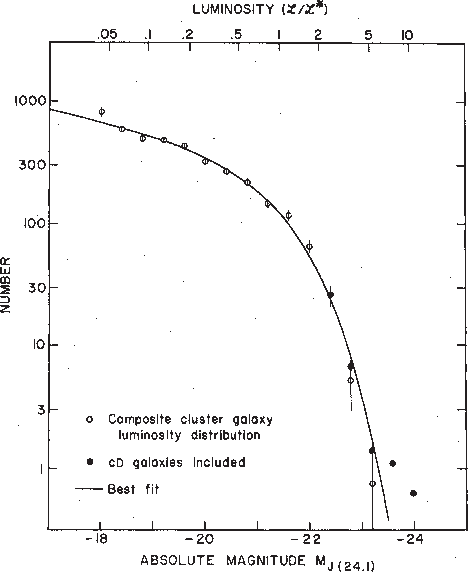
\includegraphics[width=0.4\textwidth]{schechter76}
    \caption{Fonction de luminosité des galaxies dans les amas d'Abell
      (Schechter, 1976).} 
    \label{schechter76}
  \end{SCfigure}
\end{Exercise}

\begin{Answer}
  \begin{enumerate}
  \item Cette fonction empirique montre bien la prédominance des
    galaxies de faible luminosité intrinsèque. Noter que le nombre
    total de galaxies $N_{T} = \int_{0}^{\infty} \Phi(L)\,\d L =
    \Phi^{*}\Gamma(\alpha+1)$ diverge pour $\alpha \leq -1$, mais que
    la luminosité totale $L_{T} = \int_{0}^{\infty} L\Phi(L)\,\d L =
    \Phi^{*}L^{*}\Gamma(\alpha+2)$ reste finie.
  \item On a $\Phi(L)\,\d L = \Phi(M)\,\d M$ avec $M - M^{*} = -2,5\log
    L/L^{*}$, d'où:
    $$
    \Phi(M) = 0,4 \ln 10\times \Phi^{*}\,10^{-0,4(\alpha
      +1)(M-M^{*})}\exp \left( -10^{-0,4(M-M^{*})} \right)
    $$
  \end{enumerate}

  \begin{SCfigure}[0.5]%[htp]
    \centering
    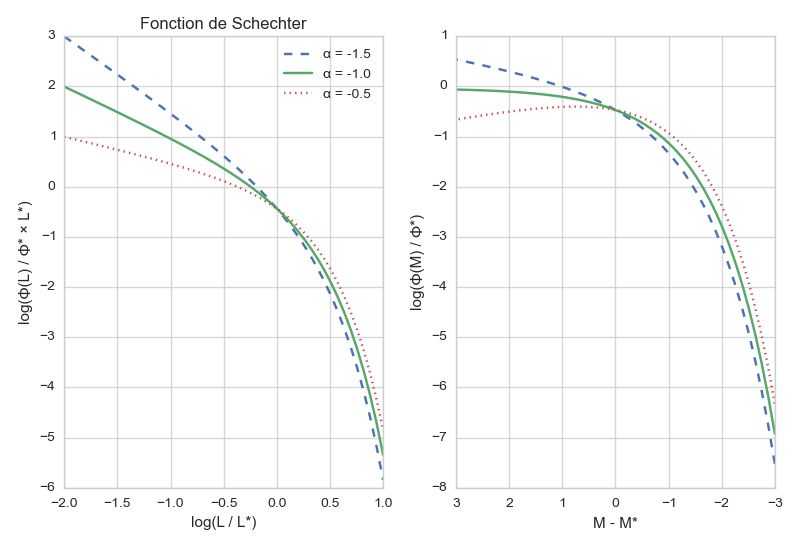
\includegraphics[width=0.6\textwidth]{schechter}
    \caption{Fonction (normalisée) de Schechter pour différentes
      valeurs de $\alpha$.}
    \label{schechter}
  \end{SCfigure}
\end{Answer}

%\subsubsection{Effets d'environnement, collisions et fusions}

\begin{Exercise}[Fréquence de collision dans un amas]
  On considère un amas de galaxies ayant les caractéristiques
  suivantes :
  \begin{itemize}
  \item il est supposé sphérique, de diamètre $D_{a}$,
  \item il contient $N_{g}$ galaxies identiques et réparties
    uniformément dans l'amas,
  \item les galaxies sont supposées animées d'une vitesse quadratique
    moyenne $v_{g}/\sqrt{2}$ (la vitesse \emph{relative} quadratique
    moyenne est donc $v_{g}$).
  \end{itemize}

  \begin{enumerate}
  \item Donner l'expression de la densité numérique de galaxies (le
    nombre par unité de volume) $n_{g}$ dans l'amas.

  \item On suppose que les galaxies ont un diamètre typique
    $d_{g}$. En modélisant les galaxies comme des sphères dures
    («~boules de billard~»), donner l'expression de la section
    efficace $S_{\mathrm{eff}}$ lors d'une interaction (collision)
    entre deux galaxies.

  \item Donner l'expression du nombre d'interactions que subit une
    galaxie de l'amas pendant un temps $\Delta t$. En déduire, pour
    une galaxie, le temps caractéristique de collision $\tau_{c}$ et
    le libre parcours moyen $\ell_{c}$.

  \item En déduire le temps $T_{c}$ entre deux interactions au sein de
    l'amas.

  \item Application numérique : considérons un amas avec $D_{a} =
    7$~Mpc, $N=850$ galaxies, $d_{g} = 20$~kpc et $v_{g} =
    650$~km/s. Explicitez le calcul numérique du temps moyen entre
    deux collisions pour cet amas.
  \end{enumerate}
\end{Exercise}

\begin{Answer}
  \begin{enumerate}
  \item Le volume de l'amas est $V_{a} = \pi D_{a}^3/6$ et la densité
    numérique de galaxies est donc $ n_{g} = N_{g}/V_{a} = 6N_{g}/\pi
    D_{a}^3$.

  \item Deux galaxies entreront en collision lorsqu'elle passent à une
    distance $< d_{g}$ l'une de l'autre. La section efficace de
    collision est donc l'aire du disque de rayon $d_{g}$ :
    $S_{\mathrm{eff}} = \pi d_{g}^{2}$.

  \item Considérons une galaxie. Le volume utile «~balayé~» par cette
    galaxie pendant le temps $\Delta t$ est $\Delta V = v_{g} \times
    S_{\mathrm{eff}} \times \Delta t$. Le nombre de collisions que
    subira cette galaxie pendant le temps $\Delta t$ est donc égal au
    nombre de galaxies dans le volume $\Delta V$ : $N_{c} = n_{g}
    \Delta V$. Le temps caractéristique de collision $\tau_{c}$
    correspond au $\Delta t$ tel que $N_{c} = 1$ ; le libre parcours
    moyen est $\ell_{c} = v_{g} \times \tau_{c}$:
    $$
    \tau_{c} = \frac{D_{a}^3}{6 N_{g} d_{g}^2 v_{g}}, 
    \qquad
    \ell_{c} = \frac{D_{a}^3}{6 N_{g} d_{g}^2}
    $$

  \item Application numérique : $v_{g} = 650\;\u{km/s} =
    665\;\u{kpc/Gan}$, $\tau_{c} = 253$~Gan, $T_{c} = \tau_{c}/N_{g} =
    297$~Man.
  \end{enumerate}
\end{Answer}


\subsection{Équilibre gravitationnel}

\begin{Exercise}[Théorème du Viriel scalaire]
  On considère le système Terre-Soleil. Le Soleil, de masse $\Msun$,
  est pris comme référence du mouvement ($v_\odot = 0$). On note
  $M_\oplus$ et $v_\oplus$ la masse et la vitesse de la Terre.
  \begin{enumerate}
  \item Écrire l'expression de l'energie cinétique du système
    Terre-Soleil.
  \item Énoncer le théorème du Viriel. En déduire l'expression de la
    distance $D$ d'équilibre entre la Terre et le Soleil. Faire
    l'application numérique, sachant que $\Msun = 2\e{30}$~kg,
    $M_\oplus = 5,97\e{24}$~kg et $v_\oplus = 30$~km/s.
  \item On considère un système d'étoiles binaires en équilibre. Pour
    simplifier, les étoiles sont prises de masses égales $M_{1} =
    M_{2} = \Msun$ et leurs vitesses sont considérées comme égales
    $v_1 = v_2 = v$.

    Expliciter la relation entre la distance entre ces deux étoiles et
    leur vitesse et calculer cette vitesse $v$ pour les distances
    d'équilibre $D$ suivantes : 1~UA, 10~UA et 100~UA.
  \end{enumerate}
\end{Exercise}

\begin{Answer}
  \begin{enumerate}
  \item $K = 1/2 M_\oplus v_\oplus^2$
  \item Théorème du Viriel : $2K + U = 0$ avec $U = -G\Msun
    M_\oplus/D$ d'où $D = G\Msun/v_\oplus^2 = 1$~UA.
  \item $K = 1/2\,M_{1}v_{1}^{2} + 1/2\,M_{2}v_{2}^{2} =
    \Msun v^{2} \stackrel{\mathrm{Viriel}}{=} -U/2 =
    +G\Msun^{2}/(2D)$ d'où $v = \sqrt{G \Msun/(2 D)}$, soit:
    \begin{center}
      \begin{tabular}{lccc}
        \toprule
        $D$ [UA]   & 1    & 10  & 100 \\
        \midrule
        $v$ [km/s] & 21,1 & 6,7 & 2,1 \\
        \bottomrule
      \end{tabular}
    \end{center}
  \end{enumerate}
\end{Answer}

\begin{Exercise}[Autres applications du théorème du Viriel]
  On va maintenant utiliser le théorème du Viriel pour remplir le
  tableau ci-dessous, donnant les rayons, masses et vitesse
  caractéristiques de différents système stellaires.  
  \begin{center}
    \begin{tabular}{lrrr}
      \toprule
      Système & $R$ & $V$ [km/s] & $M/\Msun$ \\ 
      \midrule
      Amas globulaire  & 10~pc  & 10   & \corrige{$4,6\e{5}$} \\ 
      Galaxie          & 15~kpc & 200  & \corrige{$2,8\e{11}$} \\ 
      Amas de galaxies & 1~Mpc  & 1000 & \corrige{$4,6\e{14}$} \\ 
      \bottomrule
    \end{tabular}
  \end{center}
\end{Exercise}

\begin{Answer}
  On a $U = -GM^{2}/(2R)$ et $K=1/2\, MV^{2}$ d'où $M = 2RV^{2}/G$,
  avec $G = 6,67\e{-11}\;\u{m^{3}~kg^{-1}~s^{-2}} =
  4,302\e{-3}\;\u{km^{2}~s^{-2}~pc~\Msun^{-1}}$.
\end{Answer}

\begin{Exercise}[Temps cinématique]
  On va maintenant calculer le temps cinématique $t_c$ pour différents
  systèmes stellaires. 
  \begin{center}
    \begin{tabular}{lrrr}
      \toprule
      Système & $R$ & $M/\Msun$ & $t_c$ [ans] \\ 
      \midrule
      Amas ouvert      & 1~pc   & 500      & \corrige{$9,4\e{5}$} \\ 
      Amas globulaire  & 10~pc  & $10^5$   & \corrige{$2,1\e{6}$} \\ 
      Galaxie          & 15~kpc & $10^{11}$ & \corrige{$1,2\e{8}$} \\ 
      Amas de galaxies & 1~Mpc  & $10^{14}$ & \corrige{$2,1\e{9}$} \\
      \bottomrule
    \end{tabular}
  \end{center}
  Que remarquez-vous sur ces temps cinématiques pour les différents
  systèmes ?
\end{Exercise}

\begin{Answer}
  $t_{c} = R/V = \sqrt{2R^{3} / GM}$ avec $G =
  4,500\e{-15}$~\u{pc^{3}~\Msun^{-1}~an^{-2}}.

  Les temps cinématiques pour un amas ouvert et un amas globulaire ne
  sont pas vraiment différents malgré leurs tailles respectives très
  différentes.  De même entre une galaxie et un amas globulaire : il
  ne faut qu'environ 100$\times$ plus de temps à une étoile avec une
  vitesse typique pour traverser une grosse galaxies qu'un amas
  globulaire (bien sur les vitesses caractéristiques ne sont pas les
  mêmes pour ces deux systèmes).
\end{Answer}

% ==============================================================================

\chapter{Cosmologie}

\section{Espace et temps absolus}

\begin{Exercise}[La faiblesse de la force de gravitation]
  Marcel et Naomi ressentent l'un pour l'autre une certaine
  attirance...  Quelle part en revient tout bêtement à la force de
  gravitation universelle, lorsque leurs centres de gravité respectifs
  sont distants de 1 mètre ?  Quelle masse $m$, au même point de la
  Terre, présente un poids égal à cette force ?  Marcel pèse 700~N, et
  Naomi 580~N.  Le rayon de la Terre sera supposé égal à $R_{\oplus} =
  6370$~km, et la masse de la Terre est de $M_{\oplus} =
  5,97\e{24}$~kg.
\end{Exercise}

\begin{Answer}
  Il s'agit d'appliquer la formule de Newton deux fois pour trouver
  les masses respectives de Marcel et Naomi, puis une troisième fois
  pour calculer l'attraction qui s'exerce entre eux: $F_{MN} = G\,m_M
  m_N/d^2 = G\,m M_{\oplus}/R_{\oplus}^2$.  Pour Marcel,
  $P_{\mathrm{M}} = G M_{\mathrm{M}}M_{\oplus} / R_{\oplus}^2$ soit
  $M_{\mathrm{M}} = P_{\mathrm{M}}R_{\oplus}^2 / (G M_{\oplus}) =
  71,3~\u{kg}$. Pour Naomi, on peut utiliser le fait que
  $M_{\mathrm{N}}/M_{\mathrm{M}} = P_{\mathrm{N}} / P_{\mathrm{M}}$,
  puisque les deux personnes sont soumises au même champ de gravité,
  donc $M_{\mathrm{N}} = M_{\mathrm{M}}\times
  P_{\mathrm{N}}/P_{\mathrm{M}} = 71,3 \times 580/700 = 59,0~\u{kg}$
  d'où $F_{\mathrm{NM}} = 2,81\e{-7}~\u{N}.$ La masse qui présente un
  poids égal à cette valeur est de $m =
  F_{MN}R_{\oplus}^{2}/(GM_{\oplus}) = 2,86\e{-8}\;\u{kg} =
  \SI{28,6}{\micro g}$.

  L'attraction gravitationnelle est une force \emph{très faible},
  c'est même la plus faible des quatre forces fondamentales de
  l'Univers.
\end{Answer}

% \subsection{Problèmes de l'Univers de Newton}

% \begin{Exercise}[L'instabilité gravitationnelle]
%   Pourquoi Newton pense-t-il que ces trois hypothèses supplémentaires
%   permettraient, chacune, de «~sauver~» l'Univers de la catastrophe
%   gravitationnelle ?
% \end{Exercise}

% \begin{Answer}
%   \begin{itemize}
%   \item Si l'Univers est infini, tout point est entouré d'une
%     distribution de matière à symétrie sphérique, et restera donc
%     immobile.
%   \item Si l'Univers est en expansion, c'est qu'il n'est pas en train
%     de se contracter !
%   \item Si l'Univers est très jeune, il n'a pas encore eu le temps de
%     démarrer sa contraction gravitationnelle de façon sensible.
%   \end{itemize}
% \end{Answer}

% \begin{Exercise}[Le paradoxe d'Olbers]
%   En quoi le fait que l'Univers soit jeune et en expansion peut-il
%   permettre d'expliquer la noirceur du ciel nocturne ?
% \end{Exercise}

% \begin{Answer}
%   \begin{itemize}
%   \item Si l'Univers est jeune, du fait de la vitesse finie de
%     propagation de la lumière, celle qui provient des objets très
%     lointains n'a pas eu le temps de nous parvenir.
%   \item Si l'Univers est en expansion, la lumière qui nous parvient
%     des objets très lointains a été affaiblie par cette expansion
%     (ceci sera traité plus loin dans le cours), au point de ne pas
%     être détectable.
%   \end{itemize}
% \end{Answer}

\section{La rupture relativiste}

% \subsection{Vitesse de la lumière}

% \begin{Exercise}[La première mesure de $c$]
%   Si Roemer a fait le calcul (ce que l'on ignore, mais cela semble
%   assez probable), et en supposant qu'il utilisait la même valeur de
%   la distance Terre-Soleil que les astronomes d'aujourd'hui, quelle
%   valeur de $c$ a-t-il obtenue ?
% \end{Exercise}

% \begin{Answer}
%   Si la lumière met $8+8 = 16$~min pour traverser l'orbite de la
%   Terre, c'est à dire pour franchir une distance de 2~U.A., sa
%   vitesse est $c = 2 \times 1,49598\e{11} / ( 16 \times 60 ) =
%   3,11\e{8}$~m/s. Ceci suppose que la valeur de l'U.A. admise alors
%   était la même qu'aujourd'hui, ce qui n'est certainement pas exact
%   : en 1675, on n'avait pas encore très bien mesuré la distance de
%   la Terre au Soleil... La valeur de deux fois huit minutes est
%   elle-même approximative. Roemer aurait plutôt trouvé $2\e{8}$~m/s,
%   dit-on. La première détermination sérieuse de l'Unité Astronomique
%   est due à Cassini et Richer, en 1671. Il faudra attendre le XXe
%   siècle et les méthodes d'écho radar pour disposer de mesures très
%   précises de cette valeur.
% \end{Answer}

\subsection{Relativité générale}

\begin{Exercise}[L'équivalence gravité/accélération]
  Pour la Relativité Générale, gravitation et accélération sont
  équivalentes, mais cette équivalence n'est que \emph{locale}: aucune
  expérience de physique ne permet de distinguer les effets de l'une
  de ceux de l'autre, \emph{à condition} de se limiter à un «~petit~»
  domaine spatial.

  En reprenant l'expérience de pensée de l'«~ascenseur d'Einstein,~»
  pouvez-vous montrer qu'il est en effet facile de distinguer
  pesanteur et accélération par la fusée si on abandonne la localité.
\end{Exercise}

\begin{Answer}
  À grande échelle, le champ de gravité qui environne un corps massif
  reste en général discernable d'une accélération constante.  Par
  exemple, dans l'image de l'ascenseur d'Einstein, il ne faut pas que
  la cabine soit trop étendue.  Sinon, le parallélisme ou le
  non-parallélisme des forces sur des masses éloignées l'une de
  l'autre trahirait la «~vraie~» nature du champ.  Sur la
  Fig.~\ref{grav}, la cabine de gauche, supposée accélérée vers le
  haut (flèche bleue), produit des forces parallèles (flèches rouges)
  sur les deux masses-test.  La cabine de droite, immobile dans le
  champ de gravitation de la Terre, montre des forces convergentes
  vers le centre de la Terre (flèches vertes).  De même, le physicien
  pourrait mettre en évidence une dépendance de la force avec
  l'altitude dans le cas de droite.
  \begin{SCfigure}%[htp]
    \centering
    \includegraphics[width=0.4\textwidth]{grav}
    \caption{}
    \label{grav}
  \end{SCfigure}
\end{Answer}

\subsection{Les tests}

\begin{Exercise}[Le décalage gravitationnel vers le rouge]
  Une lampe spectrale émettant dans la raie H$\alpha$ ($\lambda_{0} =
  656,3$~nm) est utilisée pour communiquer à partir d'une capsule en
  orbite serrée autour d'une étoile à neutrons. Le rayon de l'orbite
  est $R=1000$~km, la masse de l'étoile de $M=1,5$~\u{\Msun}.  À
  quelle longueur d'onde $\lambda$ le vaisseau qui a lancé la capsule,
  et se tient prudemment à grande distance, doit-il rechercher les
  signaux ?

  Comparer cet effet gravitationnel au décalage par effet Doppler du
  signal de la sonde en orbite circulaire autour de l'étoile à
  neutrons.
\end{Exercise}

\begin{Answer}
  Le décalage gravitationnel subi à la distance $R$ d'un corps de
  masse $M$ s'écrit :
  \begin{align*}
    z_{G} &= \frac{GM}{c^2 R} = \frac{ 6,672\e{-11} \times 1,5 \times
      1,989\e{30} }{ 299792458^{2}\e{6} } = 2,216\e{-3} \\
    &= \frac{\lambda - \lambda_{0}}{\lambda_0}
  \end{align*}
  d'où $\lambda = (1+z_{G})\lambda_0 = 1,00221 \times 656,3 = 657,75$~nm.

  La vitesse de l'orbite circulaire de rayon $R$ autour d'une masse
  $M$ est donnée (dans l'approximation non-relativiste) par:
  $$
  v = \sqrt{\frac{GM}{R}} = 14112\;\u{km/s} \simeq 4,71\e{-2} \times c
  $$
  Le décalage par effet Doppler (dans la même approximation non
  relativiste) est donc $z_{D} = v/c = \sqrt{z_{G}} \gg z_{G}$.
\end{Answer}


\section{Le Big Bang}

\subsection{Film des débuts}

\begin{Exercise}[Nucléosynthèse primordiale ou non ?]
  Les éléments légers $\mathrm{H}$, ${}^{2}\mathrm{H}$,
  ${}^{3}\mathrm{H}$, ${}^{4}\mathrm{He}$, ${}^{7}\mathrm{Li}$ sont
  nés avec le Big Bang. Mais d'où proviennent tous les autres éléments
  «~lourds~», ceux qui entrent dans la composition des objets du
  quotidien ?
\end{Exercise}

\begin{Answer}
  Les chapitres traitant des modèles stellaires et de l'évolution
  stellaire nous fournissent la réponse :
  \begin{itemize}
  \item Jusqu'au ${}^{56}\mathrm{Fe}$, les noyaux sont produits par
    les étoiles.  La source d'énergie de celles-ci est d'origine
    thermonucléaire, et elles sont des usines à fabriquer, par fusion,
    des noyaux lourds à partir de noyaux plus légers.
  \item Au-delà, seules les explosions de supernovae atteignent des
    températures suffisantes (plusieurs $10^9$~K) pour pouvoir
    synthétiser les noyaux très lourds, jusqu'aux éléments
    transuraniens.
  \item Quelques noyaux particuliers (${}^{6}\mathrm{Li}$,
    ${}^{9}\mathrm{Be}$, ${}^{10}\mathrm{B}$) sont sans doute formés
    lors des collisions des rayons cosmiques avec la matière
    interstellaire.
  \end{itemize}
\end{Answer}

\subsection{Expansion de l'Univers...}

\begin{Exercise}[... limitée par \emph{c} ?]
  Plus une galaxie est éloignée de notre Voie Lactée, plus les
  astronomes lui trouvent une vitesse d'éloignement élevée. C'est
  l'expansion de l'Univers. Mais, quand la distance croît sans cesse,
  elle atteint un moment une valeur $d_c$ telle que :
  $$
  V = H_0 d_c > c
  $$
  Étonnant, non ?
\end{Exercise}

\begin{Answer}
  Il est interdit par la Relativité Générale de mesurer une vitesse
  égale ou supérieure à $c$ pour un objet de masse non nulle, comme
  une galaxie. Cependant, cette limite ne s'applique pas à l'expansion
  de l'Univers, où les objets (p.ex. les galaxies) sont immobiles dans
  un espace dont la géométrie s'étire. Les galaxies très lointaines
  voient effectivement leur vitesse apparente atteindre celle de la
  lumière, et disparaissent alors de l'Univers observable. Ceci
  n'enlève rien au fait qu'elles continuent à s'éloigner de nous à des
  vitesses supérieures à $c$.  Signalons que nos moyens d'observation
  actuels sont loin de nous permettre d'observer les objets qui
  s'approchent de cette limite.
\end{Answer}

\begin{Exercise}[... la même partout ?]
  La radiogalaxie 3C~171 (la 171e entrée dans le troisième catalogue
  de radiources établi par l'observatoire de Cambridge) est
  relativement lointaine; entraînée par l'expansion de l'Univers, elle
  présente une vitesse de fuite de 63\,000~km/s.

  Montrer que malgré cela, l'astronome Pr.~Snurp, qui a là-bas
  découvert l'expansion de l'Univers, comme Hubble l'a fait pour nous,
  a lui aussi trouvé une loi qui s'écrit :
  $$
  v_0 = X_0 d_{0},
  $$
  $v_0$ étant la vitesse mesurée à partir de 3C~171 pour une galaxie
  lointaine située à la distance $d_0$ de 3C~171, et que la constante
  de Snurp $X_0$ partage la valeur de $H_{0}$.

  Ainsi, d'une planète de 3C~171, comme de la Terre, on observe la même
  expansion universelle, avec la même géométrie, et le même taux...
\end{Exercise}

\begin{Answer}
  Désignons par $v_T$ et $d_T$ les vitesses et distances mesurées à
  partir de la Terre, $v_{3C}$ et $d_{3C}$ celles mesurées à partir de
  3C~171.  La vitesse de récession de 3C~171 mesurée de la Terre est
  donc $v_T(3C\;171) = 63\;000$~km/s.

  Considérons une autre galaxie, $G$, observée à la fois de la Terre
  et de 3C~171. On peut écrire :
  \begin{align*}
    \vec{v}_{3C}(G) &= \vec{v}_{3C}(T) + \vec{v}_{T}(G) \\
    &= -\vec{v}_{T}(3C\;171) + \vec{v}_{T}(G) \\
    &= -H_0\vec{d}_{T}(3C\;171) + H_0\vec{d}_{T}(G) \\
    &= H_0 \left[ \vec{d}_{T}(G) - \vec{d}_{T}(3C\;171) \right ] \\
    &= H_0 \vec{d}_{3C}(G)
  \end{align*}
  et donc, à partir de 3C~171 comme de la Terre, toute les galaxie
  observée semble s'enfuir avec une vitesse proportionnelle à sa
  distance, et le facteur de proportionnalité (la constante de Snurp)
  est universel : $X_0=H_0$ (Fig.~\ref{H0}).

  \begin{SCfigure}%[htp]
    \centering
    \includegraphics[width=0.4\textwidth]{351922_281}
    \caption{}
    \label{H0}
  \end{SCfigure}
\end{Answer}

\subsection{Constante de Hubble \& Co.}

Dans les exercices suivants, on supposera la constante de Hubble égale
à $H_0 = 70$~\u{km~s^{-1}~Mpc^{-1}}.

\begin{Exercise}[Le facteur d'expansion de l'espace]
  La constant de Hubble $H_0$ est usuellement exprimée en kilomètres
  par seconde et par mégaparsec, mais cela ne parle guère au sens
  commun.  Quelle est la valeur de l'accroissement annuel d'un
  kilomètre ?
\end{Exercise}

\begin{Answer}
  $1\;\u{Mpc} = 3,09\e{19}\;\u{km}$ et $1\;\u{an} = 3,16\e7\;\u{s}$,
  donc $71\;\u{km~s^{-1}~Mpc^{-1}} = 2,27\e{-18}\;\u{km~s^{-1}~km^{-1}}
  = 71,6\;\u{nm~an^{-1}~km^{-1}}$.
\end{Answer}

\begin{Exercise}[Temps de Hubble]
  Calculez le temps de Hubble $t_{H} = 1/H_{0}$. Quelle est sa
  signification physique ?  Quelle conclusion pouvez-vous en tirer sur
  l'âge de l'Univers ?
\end{Exercise}

\begin{Answer}
  Le temps de Hubble est défini par $1/t_{H} = H_0 =
  70\;\u{km~s^{-1}~Mpc^{-1}} = 2,27\e{-18}\;\u{s^{-1}}$ d'où $t_{H} =
  4,41\e{17}~s \simeq 13,97\e{9}$~ans. Il représente l'âge de
  l'Univers dans le cas d'un taux d'expansion \emph{constant}. On peut
  donc penser que l'Univers est âgé d'environ 14~Gans.
\end{Answer}

\begin{Exercise}[Densité critique]
  Calculer la densité critique $\rho_{C} = \dfrac{3 H_{0}^{2}}{8\pi G}$.
  Quelle est sa dimension ?  La convertir en nucléons/$\u{m^{3}}$ ($m_{p}
  \simeq m_{n} \simeq m_{u} = 1,66\e{-27}$~kg), puis en $\Msun/\u{Mpc}^{3}$.
  Commenter.
\end{Exercise}

\begin{Answer}
  $\rho_{C} = 9,20\e{-27}~\u{kg\;m^{-3}} = 5,54\;\text{nucléons}\;\u{m^{-3}} =
  1,34\e{11}\;\Msun\;\u{M\pc}^{-3}$, soit environ une galaxie (massive) par
  \u{M\pc^{3}}, densité caractéristique de l'Univers local.
\end{Answer}

\begin{Exercise}[Âge de l'Univers]
  À partir de la définition de $H_0$ et de la relation $R \propto
  t^{2/3}$ entre le facteur d'échelle $R$ et le temps $t$ dans le cas
  d'un Univers euclidien ($k=0$) dominé par la matière
  ($\Omega_{M}=1$, $\Omega_{\Lambda}=0$), trouver la relation entre
  $H_{0}$ et $t$.
\end{Exercise}

\begin{Answer}
  \begin{align*}
    H_0 &\defeq \frac{1}{R}\frac{\d R}{\d t} \\
    &= \left ( \frac{t}{t_0} \right )^{-2/3} \times
    \frac{\d\left( t/t_0 \right )^{2/3}}{\d t} 
    = \left ( \frac{t}{t_0} \right )^{-2/3} \times
    \left( \frac{t}{t_0} \right)^{-1/3} \frac{2}{3} \frac{1}{t_0} 
    = \left( \frac{t}{t_0} \right)^{-1} \times \frac{2}{3t_0} \\
    &= \frac{2}{3t} \\
    \text{donc}\quad t &= \frac{2}{3\,H_{0}}
  \end{align*}
  Pour un Univers critique dominé par la matière, l'âge de l'Univers
  est égal aux deux-tiers du temps de Hubble.
\end{Answer}

\section{Modèles cosmologiques}

\begin{Exercise}[Modèle FLRW]
  Dans le cas d'un Univers de Friedmann-Lemaître-Robertson-Walker à
  courbure spatiale nulle ($k=0$), on a :
  \begin{equation}
    \left(\frac{\dot{R}}{R}\right)^{2} = 
    \frac{\Lambda}{3} + \frac{8\pi G}{3}\rho.
    \label{eq:1}
  \end{equation}
  Par ailleurs, l'équation de conservation de l'énergie s'écrit
  toujours:
  \begin{equation}
    \label{eq:2}
    \dot{\rho} = -3\left(\rho + \frac{P}{c^{2}}\right)\frac{\dot{R}}{R}.
  \end{equation}

  \begin{enumerate}
  \item Que signifient les différents termes -- $R$, $\Lambda$, $\rho$
    -- de l'équation~(\ref{eq:1}) ? Quelle est la dimension de
    $\dot{R}/R$ ?  Comment s'appelle cette quantité ?

  \item Si l'on considère le fluide parfait dont l'équation d'état --
    reliant la pression $P$ à la densité $\rho$ -- est donnée par $P =
    w\rho c^{2}$, que devient l'équation~(\ref{eq:2}) ? Vérifier que
    l'on obtient alors, en notant $\rho(R_{0}) = \rho_{0}$ :
    $$
    \frac{\rho}{\rho_{0}} = \left(\frac{R}{R_{0}}\right)^{-3(1+w)}.
    $$

  \item Dans le cas où $\Lambda = 0$, en déduire que $R$ est régit par
    une équation différentielle du type :
    $$
    \dot{R} = \alpha R^{-\eta},
    $$
    avec $\eta = (1+3w)/2$. Expliciter la valeur de $\alpha$.

  \item On peut montrer que la solution générale de l'équation
    différentielle précédente est de la forme :
    $$
    \frac{R}{R_{0}} = \left(\frac{t}{t_{0}}\right)^{\gamma}.
    $$
    Déterminer $\gamma$ en fonction de $\eta$, puis de $w$.

  \item Exprimer alors $\dot{R}/R$ en fonction de $t$.

  \item Dans le cas d'un Univers dominé par la matière ($w=0$),
    comment est relié l'âge de l'Univers $t_{0}$ à la constante de
    Hubble $H_{0}$ ? Même question dans le cas d'un univers dominé par
    les radiations ($w=1/3$).
  \end{enumerate}
\end{Exercise}

\begin{Answer}
  \begin{enumerate}
  \item $R$ : facteur d'échelle, $\Lambda$ : constante cosmologique,
    $\rho$ : densité massique.  $\dot{R}/R$ a la dimension de
    l'inverse d'un temps, c'est la constante de Hubble $H$.

  \item $\dot{\rho} = -3(1+w) H$. On vérifie que $\rho/\rho_{0} =
    (R/R_{0})^{-3(1+w)}$ est bien solution de cette équation.

  \item En introduisant la solution précédente dans
    l'éq.~(\ref{eq:1}), on obtient $\dot{R} = \alpha R^{-\eta}$ avec
    $$
    \alpha = 
    \left( \frac{8\pi G}{3}\rho_{0}R_{0}^{3(1+w)} \right)^{1/2}
    \qquad\text{et}\qquad \eta = \frac{1+3w}{2}
    $$

  \item En égalisant les expressions de $\dot{R}$, on obtient
    $$
    \gamma = \frac{1}{1+\eta} = \frac{2}{3(1+w)}.
    $$

  \item On a
    $$
    H = \frac{\dot{R}}{R} = \frac{\gamma}{t} =
    \frac{2}{3(1+w)}\frac{1}{t}.
    $$

  \item Pour $w=0$, $t_{0} = 2/(3 H_{0})$ ; pour $w=1/3$, $t_{0} =
    1/(2 H_{0})$.
  \end{enumerate}
\end{Answer}

\begin{Exercise}[\emph{Redshift} cosmologique]
  La radiogalaxie 4C~41.17 montre une raie spectrale intense à
  582,2~nm.  Cette raie est identifiée comme la raie Lyman~$\alpha$ de
  l'hydrogène. En laboratoire, sur la Terre, la longueur d'onde de
  cette raie est de 121,5~nm.

  \begin{enumerate}
  \item Quel est le redshift de la radiogalaxie 4C~41.17 ?
  \item Quel était le facteur d'échelle de l'Univers à l'époque où les
    atomes d'hydrogène de 4C~41.17 émettaient cette raie ?
  \item À quelle époque $t_{em}$ la radiogalaxie 4C~41.17 de
    l'exercice précédent a-t-elle émis la lumière que nous recevons
    aujourd'hui à $t_0$ ? On supposera un Univers critique dominé par
    la matière, avec un âge de $t_0 = 13,5\e9$~ans.
  \end{enumerate}
\end{Exercise}

\begin{Answer}
  \begin{enumerate}
  \item $1 + z = \lambda_{\text{observé}}/\lambda_{\text{émis}} =
    582,2/121,5 = 4,792$ donc $z = 3,792$.
  \item Par ailleurs, $1 + z =
    \lambda_{\text{observé}}/\lambda_{\text{émis}} =
    R_0/R_{\text{émission}}$, soit $R_{e}/R_{0} = \lambda_{0}/\lambda
    = 121,5/582,2 = 0,209$.  À l'époque où 4C~41.17 émettait la
    lumière qui nous parvient aujourd'hui, l'Univers était cinq fois
    moins «~étiré~» qu'aujourd'hui.
  \item Pour un Univers critique dominé par la matière, $R(t)/R_{0} =
    (t/t_0)^{2/3}$, et donc $t_{e} = t_0 \times
    \left(R_{em}/R_{0}\right)^{3/2}$, soit $t_{e} = 13,5 \times
    0,209^{3/2} = 1,29\e{9}$~années.  4C~41.17 émettait la lumière qui
    nous parvient aujourd'hui alors que l'Univers n'était âgé que de
    1,29 milliards d'années.
  \end{enumerate}
\end{Answer}

\begin{Exercise}[Temps de vol, distance, et expansion...]
  Il y a dix milliards d'années, ce photon que nous recevons
  aujourd'hui a quitté une lointaine galaxie.
  \begin{enumerate}
  \item Cette galaxie se trouvait-elle à dix milliards
    d'années-lumière de nous au moment de l'émission ?
  \item Cette galaxie se trouve-t-elle aujourd'hui à dix milliards
    d'années-lumière de nous ?
  \end{enumerate}
\end{Exercise}

\begin{Answer}
  \begin{enumerate}
  \item Le photon a voyagé pendant dix milliards d'années en luttant
    contre l'expansion de l'espace qui contrariait son mouvement; tout
    se passe comme s'il avait parcouru à la vitesse $c$ une distance
    supérieure à celle qui séparait la galaxie de nous au moment de
    l'émission.  Au moment de l'émission, la galaxie était donc à
    moins de dix milliards d'années-lumière de nous.
  \item Depuis que le photon a quitté la galaxie, celle-ci, entraînée
    par l'expansion, a continué à s'éloigner de nous. Le photon a bien
    parcouru (de son point de vue, en admettant qu'il en ait un) dix
    milliards d'années-lumière, puisque sa vitesse par rapport à
    l'espace est à tout instant égale à $c$, mais la galaxie a
    continué sa route pendant tout ce temps, et se trouve aujourd'hui
    à plus de dix milliards d'années-lumière de nous...
  \end{enumerate}
\end{Answer}

% ==============================================================================

\chapter{Retour sur Terre: nos repères dans le ciel}

\section{Se positionner dans le ciel}

\begin{Exercise}[Repérage]
  \begin{enumerate}
  \item Quelles sont les coordonnées horizontales des quatre points
    cardinaux ?

  \item Peut-on définir les coordonnées horizontales pour un
    observateur installé au pôle Nord géographique ou au pôle Sud ?

  \item Pour quelles valeurs de la hauteur et de la distance zénithale
    un astre est-il visible, c'est-à-dire au dessus de l'horizon ?
  \end{enumerate}
\end{Exercise}

\begin{Answer}
  \begin{enumerate}
  \item Les points cardinaux étant par définition sur l'horizon, leurs
    hauteurs sont nulles. Les directions Est-Ouest et Nord-Sud étant
    orthogonales, on a à partir de l'origine la direction Sud
    (Fig.~\ref{position}) :
    \begin{center}
      \begin{tabular}{lrr}
        \toprule
        & Azimut & Hauteur \\ 
        \cmidrule(r){2-3}
        Nord  & 180° & 0 \\ 
        Est   & 270° & 0 \\ 
        Sud   & 0°   & 0 \\ 
        Ouest & 90°  & 0 \\ 
        \bottomrule
      \end{tabular}
    \end{center}
    Remarque : L'azimut des marins est décalé de 180° par rapport à
    celui des astronomes. L'origine des azimuts est le Nord.

  \item Seule la hauteur d'un astre au-dessus de l'horizon peut être
    définie. L'azimut ne l'est pas, la ligne Nord-Sud ou le plan
    méridien étant indéterminé. La verticale du lieu est confondue
    avec l'axe de rotation de la Terre et tout plan passant par la
    verticale du pôle répond à la définition du plan méridien.

  \item Un astre n'est visible que s'il est au-dessus de l'horizon. Sa
    hauteur doit être positive par définition. Sa distance zénithale
    ($90\deg - h$) par conséquent est plus petite que 90°.  Un astre
    sous l'horizon a sa distance zénithale plus grande que 90°
    (Fig.~\ref{position2}).
  \end{enumerate}

  \begin{figure}
    \centering
    \begin{subfigure}[b]{0.4\textwidth}
      \centering
      \includegraphics[width=\textwidth]{position}
      \caption{Points cardinaux.}
      \label{position}
    \end{subfigure}
    \begin{subfigure}[b]{0.4\textwidth}
      \centering
      \includegraphics[width=\textwidth]{position2}
      \caption{Horizon et distance zénithale.}
      \label{position2}
    \end{subfigure}
    \caption{}
  \end{figure}
\end{Answer}

\section{Mouvement diurne}

\begin{Exercise}
  \begin{enumerate}
  \item Dans quelle direction se trouve un astre au moment de sa
    culmination en un lieu de latitude $+50\deg$ ?
  \item Même question pour un lieu situé à l'équateur.
  \item La hauteur d'un astre varie-t-elle au cours du mouvement
    diurne au pôle Nord ?
  \end{enumerate}
\end{Exercise}

\begin{Answer}
  \begin{enumerate}
  \item Lors du mouvement diurne, la culmination d'un astre se produit
    lorsque sa hauteur est maximale.  Suivant sa position de l'objet
    sur la sphère céleste (donc sa déclinaison), l'astre passera entre
    le zénith et le pôle (Nord pour un habitant de l'hémisphère nord
    et Sud pour...) soit entre le zénith et l'horizon opposé au pôle
    visible. À la latitude de 50°, les étoiles dont la déclinaison est
    plus petite que la latitude, la culmination se fera du côté Sud de
    l'observateur.  Pour les autres étoiles, la culmination sera du
    côté Nord (Fig.~\ref{mouvementdiurne2})

    \begin{figure}
      \centering
      \begin{subfigure}[b]{0.3\textwidth}
        \centering
        \includegraphics[width=\textwidth]{mouvement_diurne2}
        \caption{Latitude $\phi\sim 50\deg$.}
        \label{mouvementdiurne2}
      \end{subfigure}
      \begin{subfigure}[b]{0.3\textwidth}
        \centering
        \includegraphics[width=\textwidth]{mouvement_diurne3}
        \caption{Équateur ($\phi = 0$).}
        \label{mouvementdiurne3}
      \end{subfigure}
      \begin{subfigure}[b]{0.3\textwidth}
        \centering
        \includegraphics[width=\textwidth]{mouvement_diurne4}
        \caption{Pôle nord ($\phi = 90\deg$.}
        \label{mouvementdiurne4}
      \end{subfigure}
      \caption{Mouvement diurne.}
    \end{figure}

  \item L'équateur passant par le zénith, toutes les étoiles de
    déclinaisons positives culminent au Nord et les étoiles de
    déclinaisons négatives au Sud. Les étoiles de déclinaisons nulles
    passent au zénith (Fig.~\ref{mouvementdiurne3}).

  \item La verticale étant confondue avec l'axe du pôle, et l'horizon
    avec l'équateur, la déclinaison est égale à la hauteur de l'astre
    qui reste constante lors de la rotation diurne.  Seuls les objets
    de déclinaisons positives sont visibles. C'est pourquoi le Soleil
    dans son mouvement apparent durant l'année donne 6 mois
    consécutifs de jour et 6 mois consécutifs de nuit
    (Fig.~\ref{mouvementdiurne4}).
  \end{enumerate}
\end{Answer}

\begin{Exercise}[Mouvement diurne]
  \begin{enumerate}
  \item Comment varie l'azimut d'un astre au cours du mouvement
    diurne, en un lieu de latitude $+50\deg$ ? Et aussi $-50\deg$ de
    latitude. Sur la Fig.~\ref{mouvementdiurne}, on a représenté la
    situation en un lieu de l'hémisphère Sud (latitude = $-50\deg$) ;
    $P$ est alors en-dessous de l'horizon et $P'$ est au-dessus.

    \begin{SCfigure}[0.5]%[htp]
      \centering
      \includegraphics[width=0.5\textwidth]{mouvement_diurne}
      \caption{Rotation d'une étoile vue de l'hémisphère sud (latitude =
        $-50\deg$).}
      \label{mouvementdiurne}
    \end{SCfigure}

  \item Les astres se lèvent-ils du côté de l'Est et se couchent-ils
    du côté de l'Ouest aussi bien dans l'hémisphère Nord que dans
    l'hémisphère Sud ?
  \item Dans quelle direction géographique un astre culmine-t-il en un
    lieu de latitude $-50\deg$ ?
  \item Le mouvement diurne est-il observé dans le même sens pour un
    observateur de l'hémisphère Nord ou un observateur de l'hémisphère
    Sud ?
  \end{enumerate}
\end{Exercise}

\begin{Answer}
  \begin{enumerate}
  \item
    \begin{description}
    \item[Observateur de l'hémisphère Nord (latitude $+50\deg$)] On
      n'envisagera que le cas des étoiles visibles par l'observateur,
      c'est-à-dire celles dont $\delta > -(\pi/2 - \phi)$. Deux
      critères sont a envisager :
      \begin{itemize}
      \item l'étoile a une déclinaison plus grande que la latitude
        $\delta>\phi$ ou $\delta<\phi$
      \item l'étoile est circumpolaire $\delta > \pi/2 - \phi$
      \end{itemize}
      Par la première condition, si $\delta<\phi$, l'azimut de
      l'étoile varie de 0 à 360°, sinon, son azimut oscille entre une
      valeur comprise $\alpha$ entre 90 et 180° suivant sa position au
      passage au méridien et $360\deg-\alpha$. L'étoile oscille donc
      entre $\alpha$, 180° et $360\deg-\alpha$.

      Le deuxième critère (circumpolarité) indique si l'étoile a un
      lever ou un coucher, son azimut varie alors entre les positions
      des levers et couchers et celles définies par le premier
      critère.

      L'observateur orienté vers le Nord voit tourner les étoiles dans
      le sens direct autour du pôle Nord.

    \item[Observateur de l'hémisphère Sud (latitude $-50\deg$)] Les
      mêmes critères s'appliquent pour les limitations des azimuts et
      des levers et couchers, à la différence que l'azimut va osciller
      autour de la valeur 0° et que regardant le pôle Sud, il verra
      tourner les étoiles dans le sens rétrograde
      (Fig.~\ref{mouvementdiurne}).
    \end{description}
  \item Oui. Que l'on soit dans l'hémisphère Nord ou Sud, le sens de
    rotation de la Terre est le même. Les objets apparaissent à l'Est
    et se couchent à l'Ouest.

  \item Au Nord si sa déclinaison est plus grande que la latitude,
    autrement au Sud (Voir exercice 1 du même chapitre).

  \item Non (Voir exercice 4 du chapitre II).
  \end{enumerate}
\end{Answer}

\begin{Exercise}[Coordonnées horaires]
  \begin{enumerate}
  \item Quelle est la relation entre la déclinaison et la distance
    polaire d'un astre ?
  \item Quelles sont les coordonnées horaires des quatre points
    cardinaux en un lieu de latitude $\phi$ ?
  \item Que vaut la déclinaison du zénith en fonction de la latitude
    du lieu ?
  \end{enumerate}
\end{Exercise}

\begin{Answer}
  \begin{enumerate}
  \item Comme son nom l'indique, la distance polaire est l'angle entre
    la direction du pôle nord et la direction de l'objet, donc
    $p=90\deg-\delta$

  \item Table~\ref{tbl:coordonneeshoraires} et
    Fig.~\ref{fig:coordonneeshoraires}

    \begin{center}
      \begin{tabular}{lrc}
        \toprule
        & Angle horaire & Déclinaison \\ 
        \cmidrule(r){2-3}
        Sud   & 0~h  & $\phi - 90\deg$ \\ 
        Ouest & 6~h  & 0 \\ 
        Nord  & 12~h & $90\deg - \phi$ \\ 
        Est   & 18~h & 0 \\ 
        \bottomrule
      \end{tabular}
      \label{tbl:coordonneeshoraires}
    \end{center}

    \begin{figure}
      \centering
      \begin{subfigure}[b]{0.45\textwidth}
        \centering
        \includegraphics[width=\textwidth]{coordonnees_horaire}
        \caption{Points cardinaux.}
        \label{fig:coordonneeshoraires}
      \end{subfigure}
      \begin{subfigure}[b]{0.45\textwidth}
        \centering
        \includegraphics[width=\textwidth]{coordonnees_horaire2}
        \caption{Zénith.}
        \label{fig:coordonneeshoraires2}
      \end{subfigure}
      \caption{Coordonnées horaires.}
    \end{figure}

  \item La déclinaison du zénith vaut la latitude (positive pour
    l'hémisphère Nord et négative pour l'hémisphère Sud), voir
    Fig.~\ref{fig:coordonneeshoraires2}.
  \end{enumerate}
\end{Answer}

\begin{Exercise}[Coordonnées équatoriales]
  \begin{enumerate}
  \item Une étoile traverse le méridien sud à une hauteur de 85°, et
    le méridien nord à 45°. Trouver la déclinaison de l'étoile et la
    latitude de l'observateur.
  \item Où ces affirmations sont-elles vraies ?
    \begin{enumerate}
    \item Castor ($\alpha$-Gem, déclinaison $+31\deg54'$) est
      circumpolaire.
    \item Bételgeuse ($\alpha$-Ori, $7\deg24'$) culmine au
      zénith.
    \item $\alpha$-Cen ($-60\deg46'$) s'élève à une hauteur de 20° au
      méridien.
    \end{enumerate}
  \end{enumerate}
\end{Exercise}

\begin{Answer}
  \begin{enumerate}
  \item L'étoile tournant autour de la direction du pôle, les deux
    directions $OA$ et $OB$ des passages supérieur et inférieur, sont
    symétriques par rapport à l'axe $OP$. L'angle $\alpha$ égale
    l'angle $\beta$ et
    $$
    \alpha + \beta+180\deg - 45\deg -85\deg = 50\deg
    \quad\text{donc}\quad
    \alpha=\beta=25\deg
    $$
    $\alpha$ et $\beta$ sont tous deux les compléments de la
    déclinaison de l'étoile :
    $$
    \beta+\delta = 90\deg
    \quad\text{donc}\quad
    \delta=65\deg
    $$
    On calcule la latitude qui vaut la hauteur du pôle au dessus de
    l'horizon : $\phi = \alpha+45\deg = 70\deg$.

    \begin{SCfigure}%[htp]
      \centering
      \includegraphics[width=0.5\textwidth]{coordonnees_horaire3}
      \caption{Coordonnées horaires.}
      \label{fig:coordonneeshoraires3}
    \end{SCfigure}

  \item
    \begin{description}
    \item[Castor (Gem, $\delta = +31\deg56'$) circumpolaire:]
      L'étoile sera juste circumpolaire, c'est-à-dire passera tangent
      à l'horizon Nord, si sa déclinaison est le complément de la
      latitude.  Pour toute latitude plus grande, l'étoile sera plus
      élevée sur l'horizon et ne disparaîtra pas derrière celui-ci
      (Fig \ref{castor}) : $\phi>=90\deg-\delta$
      \begin{figure}[htp]
        \centering
        \begin{subfigure}[b]{0.3\textwidth}
          \centering
          \includegraphics[width=\textwidth]{castor}
          \caption{Castor.}
        \label{castor}
        \end{subfigure}
        \begin{subfigure}[b]{0.3\textwidth}
          \centering
          \includegraphics[width=\textwidth]{betelgeuse}
          \caption{Bételgeuse.}
          \label{betelgeuse}
        \end{subfigure}
        \begin{subfigure}[b]{0.3\textwidth}
          \centering
          \includegraphics[width=\textwidth]{cen}
          \caption{$\alpha$-Cen.}
          \label{cen}
        \end{subfigure}
        \caption{Coordonnées équatoriales.}
      \end{figure}

    \item[Bételgeuse (Ori, $\delta = +7\deg24'$) culmine au zénith:]
      Si l'étoile est au moment de sa culmination au zénith
      (nécessairement), sa déclinaison est égale à la latitude
      (Fig.~\ref{betelgeuse}) : $\phi=7\deg24'$

    \item[$\alpha$-Cen ($\delta = - 60\deg46'$) s'élève à une hauteur
      de +20°:] À son passage supérieur, l'étoile se trouve dans la
      configuration Fig.~\ref{cen}.  La latitude est l'angle $PON$ qui
      est égal à $P'OS$. En appliquant la relation de Chasles entre
      $P'OS$ la hauteur de l'astre 20° et la déclinaison, on obtient :
      $P'OS = 90\deg + \delta - 20\deg$ d'où $\phi = 9\deg14'$
    \end{description}
  \end{enumerate}
\end{Answer}

\section{Mouvement du Soleil}

\subsection{Année sidérale, année tropique }

\begin{Exercise}[Mouvement du Soleil, jour solaire]
  \begin{enumerate}
  \item Que valent la hauteur maximale et la hauteur minimale du
    Soleil en chacun des lieux considérés : 50°, 75°, 10°, 20° ?

  \item À quelle condition doit satisfaire la latitude d'un lieu pour
    que le Soleil n'ait ni lever ni coucher ?

  \item Comment comprendre l'expression «~soleil de minuit~» ?

  \item À quelle condition doit satisfaire la latitude d'un lieu pour
    que le Soleil puisse passer à son zénith ?

  \item Comment comprendre l'expression «~tropique du Cancer~» et «
    tropique du Capricorne~» ? on pourra discuter cette question, en
    particulier, en consultant une carte céleste.
  \end{enumerate}
\end{Exercise}

\begin{Answer}
  \begin{enumerate}
  \item Inclinaison de l'écliptique sur l'équateur :
    $\epsilon=23\deg27'$. On détermine les relations qui relient la
    latitude $\phi$, les hauteurs minimum et maximum avec les deux
    positions du Soleil en déclinaison $\pm \epsilon$.
    \begin{itemize}
    \item Position solstice hiver : $SOm = SOE - \epsilon =
      (90\deg-\phi) -\epsilon$
    \item Position solstice été : $SOm = SOE + \epsilon =
      (90\deg-\phi) +\epsilon$
    \end{itemize}
    ou le supplément si le Soleil sous les tropiques est passé de
    l'autre côté.
    \begin{center}
      \begin{tabular}{lcccc}
        \toprule
        Latitude $\epsilon$ & 50° & 75° & 10° & $-$20° \\
        Hauteur max. & $63\deg27'$ & $38\deg27'$ & $90\deg$ & $90\deg$ \\
        Hauteur min. & $16\deg33'$ & $-08\deg27'$ & $56\deg33'$ & $46\deg33'$ \\
        \bottomrule
      \end{tabular}
    \end{center}
    Attention aux positions entre les tropiques, le Soleil au solstice
    d'été pour les latitudes nord (solstice d'hiver pour les latitudes
    sud) est passé au Sud (au Nord) et de ce fait est plus bas que le
    jour où il passe au zénith au méridien (Fig.~\ref{mvtsolaire}).

    \begin{figure}
      \centering
      \begin{subfigure}[b]{0.45\textwidth}
        \centering
        \includegraphics[width=\textwidth]{mvt_soleil}
        \caption{}
        \label{mvtsolaire}
      \end{subfigure}
      \begin{subfigure}[b]{0.45\textwidth}
        \centering
        \includegraphics[width=\textwidth]{mvt_soleil2}
        \caption{}
        \label{mvtsolaire2}
      \end{subfigure}
      \caption{}
    \end{figure}

  \item Ceci se produit dans l'hémisphère nord en été quand le Soleil
    a une déclinaison suffisamment positive. On appelle ce phénomène
    le «~soleil de minuit~». Sur la figure ci-contre (cas de
    l'hémisphère Nord), lorsque au passage inférieur, l'angle $NOD$
    est positif, le Soleil ne se couche pas, son mouvement est
    circumpolaire.
    \begin{align*}
      NOD = NOE' + E'OD &> 0 \\
      90\deg - \phi &< \delta_{\odot} \\
      \phi &> 90\deg - \delta_{\odot}
    \end{align*}
    Au jour des solstices ($\delta_{\odot} = \pm 23\deg27'$) il
    suffit d'être à une latitude $\phi > 66\deg33'$ (en été pour
    l'hémisphère Nord) ou $\phi < - 66\deg33'$ (en hiver pour
    l'hémisphère Sud) ; les lieux de latitude $\phi$ égale à $\pm
    66\deg33'$ définissent sur le globe terrestre les parallèles
    appelés «~cercles polaires~» (respectivement boréal et austral)
    (Fig.~\ref{mvtsolaire2}).

  \item Vers les pôles, lors de son passage inférieur dans le plan
    méridien, le Soleil est au-dessus de l'horizon et son angle
    horaire ayant augmenté de 180° depuis sa culmination (par
    définition, il s'agit alors de «~midi~», 0~h temps solaire) vaut
    12~h, cela correspond bien à «~minuit~». À noter que le Soleil de
    minuit s'observe au Nord dans l'hémisphère boréal et au Sud dans
    l'hémisphère Sud.

  \item Pour que le Soleil passe au zénith, il faut que la déclinaison
    du zénith (qui est aussi la latitude du lieu) soit égale à celle
    du Soleil; comme cette dernière ne peut varier qu'entre
    $+23\deg27'$ et $-23\deg27'$, les lieux en question sont ceux
    de latitude comprise entre $-23\deg27'$ et $+23\deg27'$. Le
    Soleil passe au zénith de ces lieux deux fois dans le cours d'une
    année, au printemps et en été dans l'hémisphère Nord et en automne
    et en hiver dans l'hémisphère Sud. Les zones de la Terre qui
    correspondent à cette propriétés sont appelées les zones
    tropicales car situées entre le tropique nord du Cancer et le
    tropique sud du Capricorne.

  \item Pour les lieux de latitude égale à $+23\deg27'$ et
    $-23\deg27'$, le Soleil passe au zénith au moment des
    solstices. Ces lieux définissent sur le globe terrestre les
    parallèles appelés «~tropiques~» (du Cancer pour l'hémisphère Nord
    et du Capricorne pour l'hémisphère Sud). Si l'on se reporte à une
    carte du ciel, on voit qu'au moment des solstices le Soleil se
    trouve dans la direction de la constellation des Gémeaux (été) ou
    du Sagittaire (hiver). Il faudrait donc désigner les lieux en
    question par les noms : «~tropique des Gémeaux~» au lieu de
    tropique du Cancer et de même «~tropique du Sagittaire~» au lieu
    de tropique du Capricorne. L'appellation en usage a été définie il
    y a environ 3\,000~ans à une époque où le point $\gamma$ était
    dans la direction de la constellation du Bélier ; au solstice
    d'été le Soleil était bien dans la direction du Cancer et au
    solstice d'hiver dans la direction du Capricorne. Ce glissement
    est produit par la précession des équinoxes au rythme de 360° pour
    26\,000~ans, ce qui donne un effet de 42°, (soit environ un angle
    de 3~h) sur 3\,000~ans, comme on peut le lire sur la carte.
\end{enumerate}
\end{Answer}

\end{document}

%%% Local Variables:
%%% mode: latex
%%% TeX-PDF-mode : t
%%% ispell-local-dictionary: "francais"
%%% End:
"

% À faire:
% * Exercice sur la méthode Baade-Wesselink
% (p.ex. http://arxiv.org/abs/1201.3478 et références,
% http://www.eso.org/public/news/eso0432/, 2004ApJ...603..285M)
% * Ajout de la théorie MOND dans l'exo sur la matière noire

\documentclass[a4paper,10pt]{report}

% PREAMBULE ==============================

\usepackage[utf8]{inputenc}
\usepackage{lmodern}
\usepackage[T1]{fontenc}

% Utilise CMbright (sans) pour les formules
\DeclareMathVersion{sans}
\SetSymbolFont{operators}{sans}{OT1}{cmbr}{m}{n}
\SetSymbolFont{letters}{sans}{OML}{cmbrm}{m}{it}
\SetSymbolFont{symbols}{sans}{OMS}{cmbrs}{m}{n}
\SetMathAlphabet{\mathit}{sans}{OT1}{cmbr}{m}{sl}
\SetMathAlphabet{\mathbf}{sans}{OT1}{cmbr}{bx}{n}
\SetMathAlphabet{\mathtt}{sans}{OT1}{cmtl}{m}{n}
\SetSymbolFont{largesymbols}{sans}{OMX}{iwona}{m}{n}

\usepackage[cm]{fullpage}
\usepackage[francais]{babel}
\DecimalMathComma

\usepackage{microtype}

\usepackage{amsmath, amssymb}
\usepackage{textcomp}
\usepackage{gensymb}

\usepackage{enumitem}           % enumerate[resume]

\usepackage[pdftex]{graphicx}
\graphicspath{{./Figures/}}

\usepackage{booktabs}

\usepackage[rightcaption]{sidecap}
\usepackage{caption}
\usepackage{subcaption}

\usepackage{siunitx}
\sisetup{%
  detect-all,
  free-standing-units,          % create standalone commands
  locale=FR, 
  inter-unit-product={\,},      % character between units
}
\DeclareSIUnit\Lsun{\ensuremath{\mathsf{\emph{L}}_{\odot}}}
\DeclareSIUnit\Rsun{\ensuremath{\mathsf{\emph{R}}_{\odot}}}
\DeclareSIUnit\Msun{\ensuremath{\mathsf{\emph{M}}_{\odot}}}
\DeclareSIUnit\pc{pc}           % parsec
\DeclareSIUnit\as{as}           % arcsec

\usepackage{hyperref}
\hypersetup{
  pdftitle   = {Astrophysique pour la licence, fascicule de TD},
  pdfauthor  = {Yannick Copin, pour l'équipe enseignante Astro-L2},
  pdfsubject = {Astrophysique pour la licence, Université de Lyon 1},
  unicode=true,              % non-Latin characters in Acrobat’s bookmarks
  linktoc=all,
  colorlinks=true,           % false: boxed links; true: colored links
  linkcolor=OliveGreen,      % color of internal links
  citecolor=OliveGreen,      % color of links to bibliography
  urlcolor=MidnightBlue,     % color of external links
  pdfencoding=auto,          % http://tex.stackexchange.com/questions/119079
  psdextra=true,
}
\usepackage{bookmark} % http://tex.stackexchange.com/questions/119079

% Make Adobe Reader use the RGB rendering model for pages with transparency
% http://tex.stackexchange.com/questions/16061/
\pdfpageattr{/Group << /S /Transparency /I true /CS /DeviceRGB>>}

% Définition de l'environnement 'Exercise'
\newcounter{noexo}
\setcounter{noexo}{0}
\newenvironment{Exercise}[1][]{%
  \refstepcounter{noexo}
  \medskip\noindent\textbf{Exercice~\thenoexo~:~#1}
  \medskip\par
  \addcontentsline{toc}{paragraph}{Exercice~\thenoexo~:~#1}
  \label{exo:\thenoexo}
}{}

% Définition de l'environnement 'Answer'
\usepackage[usenames, dvipsnames]{color}
\usepackage{comment}
\specialcomment{Answer}{%
  \begingroup
  \sffamily\color{CadetBlue}
  \mathversion{sans}
  %\medskip\noindent\textbf{Corrigé :~}
  \paragraph*{\textsf{Corrigé :}}
}{%
  \endgroup
}
% http://tex.stackexchange.com/questions/159820/comment-sty-and-utf8-encoding
\renewcommand\ThisComment[1]{%
  \immediate\write\CommentStream{\unexpanded{#1}}
}

% Inclusion ou non des corrigés
\ifdefined\sanscorrige
  \message{Fascicule sans solutions}%
  \excludecomment{Answer} % Remove answers
  \newcommand{\corrige}[1]{}
\else
  \message{Fascicule *AVEC* solutions}%
  \newcommand{\corrige}[1]{%
    \sffamily\color{CadetBlue}\mathversion{sans}#1}
\fi

% Définitions locales
%\newcommand{\e}[1]{\ensuremath{\times 10^{#1}}}
\newcommand{\e}[1]{\ensuremath{\times 10^{#1}}}
\renewcommand{\d}{\ensuremath{\mathrm{d}}}
\renewcommand{\deg}{\ensuremath{\degree}}
\renewcommand{\vec}[1]{\ensuremath{\boldsymbol{\mathbf{#1}}}}
%\renewcommand{\u}[1]{\ensuremath{\mathrm{#1}}} % Unités
\renewcommand{\u}[1]{\si{#1}} % Unités
\newcommand{\defeq}{\mathrel{\widehat=}}
\DeclareMathOperator{\grad}{\mathbf{grad}}

\newcommand{\farcm}{%
  \mbox{\ensuremath{.\mkern-4mu^\prime}}} % fractional arcminute symbol: 0.'0
\newcommand{\farcs}{%
  \mbox{\ensuremath{.\!\!^{\prime\prime}}}} % fractional arcsecond symbol: 0.''0
\newcommand{\fdg}{%
  \mbox{\ensuremath{.\!\!\degree}}}      % fractional degree symbol: 0.°0

\newcommand{\red}[1]{\textcolor{red}{#1}}
\newcommand{\note}[1]{\fcolorbox{red}{yellow}{\color{black} #1}}

% PAGE DE TITRE ET PREAMBULE ==============================

\makeatletter
\def\thickhrulefill{\leavevmode \leaders \hrule height 1pt\hfill \kern \z@}
\renewcommand{\maketitle}{\begin{titlepage}%
    \let\footnotesize\small
    \let\footnoterule\relax
    \parindent \z@
    \reset@font
    \null
    \begin{center}
      \huge \bfseries \@title
      \ifdefined\sanscorrige
      \else
      \\\textcolor{red}{avec solutions}
      \fi
    \end{center}
    \hrule height 1pt
    \begin{flushright}
      Université Claude Bernard Lyon1 \\
    \end{flushright}
    \vfil
    \vfil
    \begin{figure}[htp]
      \centering
      \includegraphics[width=0.8\textwidth]{flammarion}
      \caption{La gravure sur bois dite «~de Flammarion~».}
    \end{figure}
    \begin{center}
    \vfil
      {\Large \@author} \\[1em]
      {\large \@date}
    \end{center}
  \end{titlepage}%
  \setcounter{footnote}{0}%
}
\makeatother

\title{Fascicule de TD}
\date{\small Version du \today}
\author{Astrophysique pour la licence\\[\medskipamount]Université Lyon 1}

\begin{document}

\maketitle

% 2: Down to subsection (no exercices)
% 4: Down to paragraph (exercices)
\setcounter{tocdepth}{4}
\tableofcontents

\newpage

% EXERCICES ET SOLUTIONS ==============================

\chapter{Vie des étoiles}

\section{La lumière des étoiles}

\subsection{Photosphère et température effective}

\begin{Exercise}[Luminosité du Soleil]
  Calculer la luminosité du Soleil à partir de sa température
  effective $T_\odot \approx \SI{5770}{K}$ et de son rayon
  $\Rsun \approx \SI{6,96e8}{m}$.
\end{Exercise}

\begin{Answer}
  Dans l'hypothèse du corps noir, la luminosité est reliée à la
  température et au rayon par $\Lsun = 4 \pi \Rsun^2 \sigma
  T_{\odot}^{4}$ avec la constante de Stefan $\sigma =
  \SI{5,67e-8}{W.m^{-2}.K^{{-4}}}$, soit $\Lsun \approx
  \SI{3,83e26}{W}$.
\end{Answer}


\begin{Exercise}[Rayon des étoiles]
  Déterminer le rayon (en unité solaire), la longueur d'onde de Wien
  et la couleur «~visible~» des étoiles suivantes :
  \begin{enumerate}
  \item Naine blanche : $L = \SI{e-2}{\Lsun}$, $T_{e} = \SI{20000}{K}$
  \item Géante rouge : $L = \SI{e2}{\Lsun}$, $T_{e} = \SI{4200}{K}$
  \item Supergéante : $L = \SI{e5}{\Lsun}$, $T_{e} = \SI{6000}{K}$
  \end{enumerate}
  Rappel de la loi de Wien : $\lambda_{\max} T = \SI{2898}{\micro\meter\K}$.
\end{Exercise}

\begin{Answer}
  \begin{center}
    \begin{tabular}{lccccl}
      \toprule
      Type stellaire & $L$~[\Lsun] & $T_{e}$~[K] &
      $R$~[\Rsun] & $\lambda_{\max}$ [nm] & Couleur \\
      \midrule
      Naine blanche & $10^{-2}$ & 20000  & 0,008 & 145 & Blanc \\
      Géante rouge  & $10^{2}$  & 4200  & 18,8   & 690 & Rouge \\
      Supergéante   & $10^{5}$  & 6000  & 291,7  & 483 & Bleu \\
      \bottomrule
    \end{tabular}
  \end{center}
\end{Answer}


\begin{Exercise}[Équilibre radiatif de la Terre]
  %\textbf{Rappel :} Le \emph{flux} est une puissance par unité de
  %surface (unités~SI : \u{J~s^{-1}~m^{-2}}).

  Soit $L$ la puissance lumineuse du Soleil, $R$ le rayon de la Terre,
  $D$ la distance Terre-Soleil et $T_{e}$ la température effective à
  la surface de la Terre :
  \begin{enumerate}
  \item Écrire la relation entre $L$ et $F(D)$, le flux lumineux à une
    distance $D$ du Soleil. En déduire la puissance lumineuse totale
    $P_{r}$ reçue par la Terre.
    % (on suppose que la terre est vue du Soleil comme un disque de
    % rayon $R$)
  \item Utiliser la loi de Stefan et expliciter le flux lumineux
    $F_e$, puis la puissance totale $P_e$, rayonnés par la Terre.
  \item Écrire l'égalité des puissance reçue et rayonnée à la surface
    de la Terre, en déduire l'expression de la température $T_{e}$ en
    fonction des données du problème.
  \item Application numérique, sachant que $L = \SI{3,85e26}{W}$, $R =
    \SI{6400}{km}$, $D = \SI{1,500e11}{m}$, $\sigma =
    \SI{5,67e-8}{W.m^{-2}.K^{-4}}$.
  \item Commenter sur la validité et les limites de ce modèle.
   \end{enumerate}
\end{Exercise}

\begin{Answer}
  \begin{enumerate}
  \item $F(D) = L / 4\pi D^2$, $P_{r} = L R^2/(4 D^2)$
  \item $F_e = \sigma T_{e}^4$ et $P_e = 4\pi R^2 \sigma T_{e}^4$
  \item $P_e = P_r$ d'où $T_{e} = \left( L / (16\pi D^2\sigma)
    \right)^{1/4} = 278$~K.
  \end{enumerate}
\end{Answer}


\subsection{Système de magnitudes}

\begin{Exercise}[Système binaire]
  Les deux composantes de l'étoile $\alpha$ du Centaure située à
  1,32~pc de distance ont des magnitudes visuelles (magnitude
  apparente dans la bande $V$) de 0,30 et 1,70. On demande :
  \begin{enumerate}
  \item Le rapport des flux des deux étoiles dans la bande $V$.
  \item La magnitude visuelle globale du système.
  \item La correction qu'il faut apporter aux magnitudes apparentes de
    ce système pour obtenir les magnitudes absolues.
  \end{enumerate}
\end{Exercise}

\begin{Answer}
  On rappelle que la magnitude apparente $m$ est liée au flux $f$ par
  $m = -2,5 \log_{10}(f / f_{0})$.
  \begin{enumerate}
  \item Le rapport des flux des deux composantes de $\alpha$~Cen
    dépend de la différence de magnitudes et vaut :
    $$
    f_2 / f_1 = 10^{(m_{1} - m_{2})/2,5} = 0,28
    $$
  \item La magnitude apparente visuelle globale du système
    $m_{\Sigma}$ se calcule à partir du flux total $f_{\Sigma} = f_{1}
    + f_{2}$ (les puissances émises par les deux composantes
    s'ajoutent) :
    $$
    m_{\Sigma} = -2,5 \log(f_{\Sigma} / f_{0}) = 
    %-2,5 \log(f_{1}/f_{0} + f_{2}/f_{0}) =
    -2,5 \log(10^{-m_{1}/2,5} + 10^{-m_{2}/2,5}) = 0,04
    $$
  \item La différence entre magnitudes apparente $m$ et absolue $M$
    correspond au module de distance $\mu$ du système :
    $$
    \mu = m - M = 5 \log(D/\SI{10}{\pc}) = -4,4
    $$
  \end{enumerate}
\end{Answer}


\section{Classification spectrale}

\subsection{Mesures des distances}

\subsubsection{Parallaxe trigonométrique}

\begin{Exercise}[Incertitude]
  Relier l'incertitude sur la distance $\Delta D$ à celle sur la
  parallaxe $\Delta p$.
\end{Exercise}

\begin{Answer}
  Il existe deux méthodes pour trouver le résultat demandé :
  \begin{itemize}
  \item En différenciant l'équation $D = 1/p$, on obtient $\d D =
    -(1/p^2)\d p$, d'où l'incertitude en prenant la valeur absolue :
    $$
    \Delta D = \frac{1}{p^2}\Delta p = \frac{D}{p}\Delta p
    \quad\text{soit finalement}\quad 
    \Delta D/D = \Delta p/p.
    $$

  \item On peut également prendre le logarithme de l'équation $D =
    1/p$, ce qui donne $\ln~D = -\ln~p$, puis on différencie :
    $\d\ln~D = -\d\ln~p$, soit $\d D/D = -\d p/p$. En prenant la
    valeur absolue, on retrouve le résultat précédent.
  \end{itemize}
\end{Answer}

\begin{Exercise}[Astrométrie spatiale]
  Considérons les deux missions d'astrométrie spatiale : Hipparcos
  (1989), avec une incertitude absolue sur la mesure de la parallaxe
  typique de $\Delta p = 2$~mas, et Gaia (2013), avec $\Delta p =
  7$~$\mu$as. Quelles sont les précisions obtenues à une distance de
  100~pc ? de 1000~pc ?  À quelle distance aura-t-on une erreur de
  100\% ?
\end{Exercise}

\begin{Answer}
  Les étoiles situées à $D = 100$~pc ont une parallaxe $p = 1/100 =
  0\farcs 01 = 10$~mas. La précision obtenue sera de
  \begin{align*}
    \text{Hipparcos:}\quad \frac{\Delta D}{D} &= \frac{\Delta p}{p} =
    \frac{2\e{-3}}{10^{-2}} = 2\e{-1} = 20 \% \\
    \text{Gaia:}\quad \frac{\Delta D}{D} &= \frac{\Delta p}{p} = 
    \frac{7\e{-6}}{10^{-2}} = 7\e{-4} = 0,07 \%
  \end{align*}
  Pour des étoiles à $D=1000$~pc, $p=1$~mas, et les précisions
  deviennent 10 fois moins bonnes : 200\% avec Hipparcos et 0,7\% avec
  Gaia.

  On aura une erreur de 100\% quand $\Delta D = D$, soit $\delta p =
  p$. La distance correspondante s'obtient donc par
  \begin{align*}
    \text{Hipparcos:}\quad D_{\max} &= 1/p = 1/2\e{-3} = \SI{500}{\pc} \\
    \qquad\text{Gaia:}\quad D_{\max} &= 1/p = 1/7\e{-6} = \SI{143}{\kilo\pc}
  \end{align*}
\end{Answer}

\begin{Exercise}[Parallaxe et magnitude absolue]
  Le tableau suivant donne la magnitude apparente $m_V$ et la
  parallaxe $p$ de trois étoiles. Calculer leur distance $D$ avec son
  incertitude, l'erreur relative sur la distance $\Delta D / D$ et
  leur magnitude absolue $M_V$.
  \begin{center}
    \begin{tabular}{lccc}
      \toprule
      & $\alpha$ CMa (Sirius) & $\alpha$ Tau (Aldebaran) & $\alpha$ Ori
      (Bételgeuse) \\
      \cmidrule(r){2-4}
      $m_V$ & $-1,47$ & $0,85$ & $0,58$ \\
      $p$ (mas) & $379,2 \pm 1,6$ & $50,1 \pm 1,0$ & $7,6 \pm 1,6$ \\
      \bottomrule
    \end{tabular}
  \end{center}
\end{Exercise}

\begin{Answer}
  \begin{center}
    \begin{tabular}{lccc}
      \toprule
      & $\alpha$ CMa & $\alpha$ Tau & $\alpha$ Ori \\
      \cmidrule(r){2-4}
      $D$ (pc) &
      $2,637 \pm 0,012$ & $19,96 \pm 0,40$ & $132 \pm 28$ \\
      $\Delta D / D$ & 0,4\% & 2\% & 21\% \\
      $M_V$ & $1,42$  & $-0,65$ & $-4,99$ \\
      \bottomrule
    \end{tabular}
  \end{center}
  Étant donné la forme de la relation donnant la distance $D$ à partir
  de la parallaxe $p$, leurs incertitudes relatives sont égales, ce
  qui permet d'avoir immédiatement $\Delta D / D$. Ces résultats
  illustrent bien la diminution de la précision lorsque la distance
  augmente.  La magnitude absolue s'obtient par la relation $M_V = m_V
  - 5~\log(D/\SI{10}{\pc})$.
\end{Answer}


\begin{Exercise}[Méthode du point convergent]
  On veut déterminer la distance de l'amas des Pléiades par la méthode
  du point convergent.
  \begin{itemize}
  \item L'étude des trajectoires des étoiles de l'amas sur plusieurs
    années a permis de situer le point convergent à $\theta = 67,9 \pm
    0,6\deg$ de la direction de l'amas.
  \item L'observation du spectre de l'étoile Alcyone, faisant partie
    de cet amas, a permis de mesurer sa vitesse radiale $v_r = 10,1
    \pm \SI{0,3}{km.s^{-1}}$.
  \item Le mouvement propre apparent de cette même étoile vaut $\mu =
    47,3 \pm \SI{0,8}{\milli\as~an^{-1}}$.
  \end{itemize}
  Déterminer la distance de l'amas.
\end{Exercise}

\begin{Answer}
  Dans la formule donnant la distance de l'amas, il faut bien faire
  attention à exprimer l'angle $\mu$ en radians et à utiliser les
  mêmes unités de distance et de temps pour les autres grandeurs.
  \begin{itemize}
  \item $\mu = 47,3 \pm 0,8~\u{mas~an^{-1}} = 
    (2,29 \pm 0,04) \e{-7}~\u{rad~an^{-1}}$
  \item $v_r = 10,1 \pm 0,3~\u{km~s^{-1}} = 
    (1,02 \pm 0,03) \e{-5}~\u{pc~an^{-1}}$
  \item $\theta = 67,9 \pm 0,6\deg = 1,19 \pm 0,01$~rad, et donc $\tan
    \theta= 2,50 \pm 0,07$.
  \end{itemize}
  Finalement, $D = v_{r}\tan\theta/\mu = 111 \pm 8$~pc. L'erreur est
  obtenue via $\d D = (\tan\theta/\mu)\d v_{r} +
  (v_{r}/\mu)(1-\tan^{2}\theta)\d\theta -
  (v_{r}\tan\theta/\mu^{2})\d\mu$.
\end{Answer}

\subsection{Classification stellaire}

\begin{SCfigure}[0.5]
  \centering
  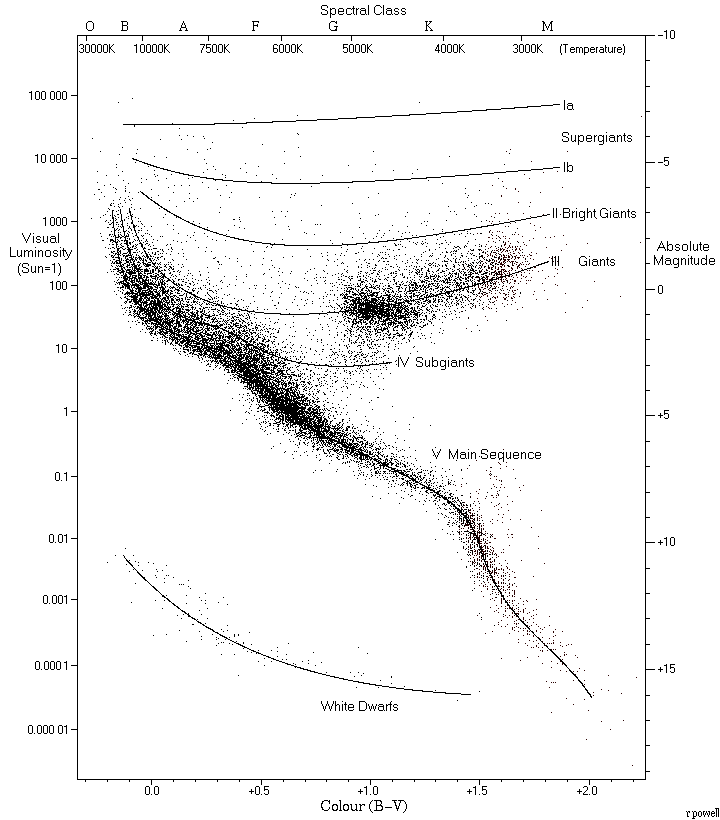
\includegraphics[width=0.5\textwidth]{hr}
  \caption{Diagramme de Hertzsprung-Russell des 22000 étoiles du
    catalogue Hipparcos et de 1000 étoiles faiblement lumineuses du
    catalogue Gliese des étoiles proches.}
  \label{hr}
\end{SCfigure}

\begin{Exercise}[Types spectraux]
  Donner approximativement le type spectral des étoiles dont le flux
  est maximal aux longueurs d'onde suivantes : 300~nm, 500~nm, et
  1,2~$\mu$m.  Peut-on déterminer la classe de luminosité ?

  Rappel de la loi de Wien : $\lambda_{\max} T = 2898$~\u{\micro m~K}.
\end{Exercise}

\begin{Answer}
  La loi de Wien permet de déterminer la température effective de
  chaque étoile, et ainsi d'en déduire une valeur approximative du
  type spectral. Ici seulement la première lettre est accessible, la
  détermination du chiffre suivant nécessiterait un tableau plus
  précis donnant les correspondances entre les sous-types et la
  température effective.
  \begin{center}
    \begin{tabular}{ccc}
      \toprule
      $\lambda_{\max}$ & $T_{\mathrm{eff}}(K)$ & Type spectral \\
      \midrule
      300 nm & 9660 & A  \\
      500 nm & 5796 & G \\
      1,2 $\mu$m & 2415 & M \\
      \bottomrule
    \end{tabular}
  \end{center}
  On ne peut pas déterminer la classe de luminosité grâce à la
  longueur d'onde du maximum du flux. Pour ceci, il faudrait connaître
  soit la luminosité de l'étoile, soit sa gravité de surface, soit son
  rayon.
\end{Answer}

\begin{Exercise}[Diagramme HR]
  Classer par ordre de température effective croissante, puis de rayon
  croissant, et enfin de luminosité croissante les étoiles de types
  spectraux suivants : M5III, O2V, K7I, A0VII.
\end{Exercise}

\begin{Answer}
  La séquence OBAFGKM décrit les types spectraux dans le sens des
  $T_{\mathrm{eff}}$ décroissantes, on aura donc dans le sens des
  $T_{\mathrm{eff}}$ croissantes : M5III, K7I, A0VII, et O2V.

  La classe de luminosité définit des groupes d'étoiles de rayon
  différent, on aura donc dans l'ordre croissant : A0VII, O2V, M5III,
  et K7I.

  Enfin, l'examen du diagramme HR montre qu'une étoile chaude de la
  séquence principale peut être plus lumineuse qu'une sous-géante
  froide, et on aura dans le sens des luminosités croissantes : A0VII,
  M5III, O2V, et K7I.

  Ceci montre que le terme «~classe de luminosité~» peut être source
  d'erreur.
\end{Answer}

\subsection{Mesure des rayons}

\begin{Exercise}[Interférométrie]
  Le tableau suivant donne le diamètre apparent $\theta_*$ des étoiles
  de l'exercice~\ref{exo:10}, mesuré par interférométrie. Calculer
  leur rayon $R$ (on rappelle les distances déterminées dans un
  exercice précédent) et, à l'aide de ce résultat, attribuer à chaque
  étoile sa classe de luminosité parmi les suivantes : I, III, V.
  \begin{center}
    \begin{tabular}{lccc}
      \toprule
      & $\alpha$ CMa & $\alpha$ Tau & $\alpha$ Ori \\
      \cmidrule(r){2-4}
      $\theta_*$ [mas] & 5,89 & 24 & 67 \\
      $d$ [pc] & 2,64  & 20  & 130 \\
      \bottomrule
    \end{tabular}
  \end{center}
\end{Exercise}

\begin{Answer}
  Pour Sirius, le rayon vaut $R[\u{UA}] = d[\u{pc}] \times
  \theta_*[''] / 2$ soit $R = \SI{7,8e-3}{ua} = \SI{1,67}{\Rsun}$.
  Le tableau suivant donne les résultats pour les 3 étoiles :
  \begin{center}
    \begin{tabular}{lccc}
      \toprule
      & $\alpha$ CMa & $\alpha$ Tau & $\alpha$ Ori \\
      \cmidrule(r){2-4}
      $R/\Rsun$ & 1,67 & 52 & 936 \\
      Classe de luminosité & V & III & I \\
      Type spectral & A1V & K5III & M2I \\
      \bottomrule
    \end{tabular}
  \end{center}
  Dans cet exemple, il est possible d'attribuer à chaque étoile sa
  classe de luminosité en utilisant le lien qui existe avec le rayon
  stellaire. Le type spectral complet est donné pour information.
\end{Answer}

\subsection{Mesure de masse (étoiles doubles)}

\begin{Exercise}[Système binaire]
  On observe une étoile double visuelle dont le plan de l'orbite est
  perpendiculaire à la ligne de visée.
  \begin{itemize}
  \item La parallaxe de ce système est de 100~mas.
  \item La plus grande séparation angulaire entre les deux composantes
    est de $5''$, et la plus petite de $1''$.
  \item La période de révolution est de 30~ans.
  % \item L'étoile primaire se trouve au foyer de l'orbite observée, car
  %   il n'y a pas d'effet de projection.
  \item Le compagnon est toujours observé à une distance du centre de
    gravité 5~fois plus grande que celle de l'étoile primaire.
  \end{itemize}
  Déterminer la masse de chaque composante.
\end{Exercise}

\begin{Answer}
  Les paramètres observés permettent de remonter aux données suivantes
  pour le système :
  \begin{itemize}
  \item La distance est $D[\u{pc}] = 1/p[''] = 10$~pc.
  \item La dimension angulaire du grand axe de l'orbite relative est
    de $5'' + 1'' = 6''$. Le demi-grand axe apparent est donc $\theta
    = 3'' = 1,45\e{-5}$~rad.
  \item Le demi-grand axe de l'orbite relative est donné par
    $a[\u{UA}] = \theta[''] D[\u{pc}]$ soit $a = 30\;\u{UA} =
    4,49\e{12}\;\u{m}$.
  \item La 3ème loi de Kepler (en unités réduites) donne la somme des
    masses : $M_{1} + M_{2} = 30\;\Msun = 5,97\e{31}$~kg.
  \item Les distances des étoiles $E_1$ et $E_2$ au centre de gravité
    $G$ vérifient $M_1 \times GE_1 = M_2 \times GE_2$. Le rapport des
    masses vaut donc $M_1 / M_2 = GE_2 / GE_1 = 5$.
  \item Finalement : $M_1 = 25\;\Msun$ et $M_2 = 5\;\Msun$
  \end{itemize}
\end{Answer}


\begin{Exercise}[Le paradoxe d'Algol]
  Le tableau suivant rappelle les caractéristiques du système binaire
  à éclipse d'Algol ($\beta$~Per):
  \begin{center}
    \begin{tabular}{lcc}
      \toprule
      $p$ (mas) & \multicolumn{2}{c}{35,14 $\pm$ 0,90} \\
      $T$ (jours) & \multicolumn{2}{c}{2,8674} \\
      $\theta_{\mathrm{rel}}$ [mas] & \multicolumn{2}{c}{2,283} \\
      \midrule
      Composantes & $A$ & $B$ \\
      \cmidrule(r){2-3}
      Type spectral & B8V & K2IV \\
      $R/\Rsun$ & 2,74 & 3,60 \\
      $\theta_{\mathrm{abs}}$ (mas) & & 1,872 \\
      \bottomrule
    \end{tabular}
  \end{center}
  On supposera l'orbite circulaire, ainsi le demi-grand axe de
  l'ellipse projetée est égal au rayon de l'orbite.

  \begin{enumerate}
  \item Quelle est la distance (et son erreur) de ce système ?
  \item Quelle est la séparation des deux étoiles ? Comparez-la à
    leurs rayons.
  \item Quelle est la masse de chacune des étoiles ? Compte-tenu des
    types spectraux, décrire le \emph{paradoxe d'Algol} et suggérer
    une solution.
  \end{enumerate}
\end{Exercise}

\begin{Answer}
  \begin{itemize}
  \item Distance : $D [\u{pc}] = 1/p[''] = 28,46 \pm 0,73$~pc.
  \item Le demi-grand axe de l'orbite relative est donné par $a
    [\u{UA}] = \theta [''] D [\u{pc}]$ soit $a = 0,065~\u{UA} =
    9,77\e{9}~\u{m} = 13,96\;\Rsun = 2,2 (R_{A}+R_{B})$.
  \item La 3ème loi de Kepler donne la somme des masses réduites
    ($\tilde{M} = M/\Msun$) : $\tilde{M}_A + \tilde{M}_B =
    \tilde{a}^3/\tilde{T}^2 = 4,46$ (avec $\tilde{a} = a[\u{UA}]$ et
    $\tilde{T} = T[\u{an}]$)
  \item Le rapport des demi-grands axes apparents de l'orbite relative
    $\theta$ et de l'orbite absolue de l'étoile secondaire $\theta_B$
    donne le rapport des masses : $\theta_B / \theta = a_B / a = M_A /
    (M_A + M_B) = 0,82$
  \item On obtient finalement les masses $M_A = 3,65\;\Msun$ et $M_B =
    0,80\;\Msun$.
  \end{itemize}
  Le tableau suivant récapitule les données physiques du système :
  \begin{center}
    \begin{tabular}{lcc}
      \toprule
      $D$ (pc) & \multicolumn{2}{c}{28,46 $\pm$ 0,73} \\
      $a/\Rsun$ & \multicolumn{2}{c}{13,96} \\
      \midrule
      & $A$ & $B$ \\
      \cmidrule(r){2-3}
      $M/\Msun$ & 3,65 & 0,80 \\
      \bottomrule
    \end{tabular}
  \end{center}
  On remarque que l'étoile la plus évoluée, $B$ ($B$ est une
  sous-géante rouge, tandis que $A$ est une étoile de la séquence
  principale) est pourtant la moins massive, ce qui est
  contre-intuitif en terme d'évolution stellaire (les étoiles les plus
  massives évoluent plus rapidement). On peut invoquer des transferts
  de masse au sein de ce système très serré pour expliquer ce
  paradoxe.
\end{Answer}

\section{Les systèmes planétaires}

\subsection{Les lois de Kepler}

\begin{Exercise}[Invariant de Runge-Lenz]
  On considère une particule $P$ de masse $m$, animée d'un mouvement
  non relativiste par rapport à un repère d'origine $O$. Ce mouvement
  est dû à un champ de forces $\vec{F} (\vec{r}) = - \grad U (r) $
  dérivant d'un potentiel central $U (r)$, où $\vec{r} = \vec{OP}$.

  À l'instant $t$ on note respectivement $\vec{v} (t)$, $\vec{a} (t)$
  et $\vec{p} (t)$ la vitesse, l'accélération et la quantité de
  mouvement de la particule $P$.

  \begin{enumerate}
  \item Montrer que la force $\vec{F}$ est radiale.
  \item Montrer que le vecteur moment cinétique $\vec{L} = \vec{r}
    \wedge \vec{p}$ est conservé au cours du mouvement.  En déduire
    que la trajectoire de $P$ est située dans un plan $\Pi$ que l'on
    caractérisera.
  \item Montrer que l'énergie mécanique $E= \dfrac{1}{2} m v^2 + U$
    est une constante du mouvement.
  \item Calculer $L$ à l'aide des coordonnées polaires $(r,\theta)$
    dans le plan $\Pi$ et en déduire la loi des aires.
  \end{enumerate}
  Dans toute la suite du problème, le potentiel est de la forme :
  $$
  U (r) = - \frac{k}{r} \qquad \text{avec} \qquad k>0
  $$
  On définit le \emph{vecteur de Runge-Lenz} :
  $$
  \vec{A} = \frac{1}{k} \, \vec{v} \wedge \vec{L} - \frac{\vec{r}}{r}
  $$
  \begin{enumerate}[resume]
  \item Montrer que le vecteur $\vec{A}$ est constant dans le temps,
    et qu'il appartient au plan $\Pi$.
  \item Montrer que :
    $$
    A^2 = 1+2 \, \frac{L^2 \, E}{mk^2}
    $$
    (On pourra utiliser les coordonnées polaires : en particulier $
    \vec{v} = v_r \, \vec{e}_r + v_{\theta} \, \vec{e}_{\theta} $).
    En déduire, lorsque $L$ est fixé, une borne inférieure pour
    l'énergie $E$.  Montrer que pour un mouvement circulaire, $E$ est
    égal à la borne inférieure.
  \item Calculer le produit scalaire $\vec{A}.\vec{r}$ en fonction de
    $L$, $m$, $k$ et $r$.  Établir alors l'équation polaire de la
    trajectoire sous la forme :
    $$
    r (\theta) = \frac{p}{1+e \, \cos \theta}
    $$
    \emph{Indication : on définira l'angle $\theta$ à partir de l'axe
      polaire dirigé selon le vecteur $\vec{A}$.}

    Vérifier que : $e =\|\vec{A}\|$ et exprimer $p$ en fonction de
    $L$, $m$ et $k$.
  \item Discuter la nature de la trajectoire suivant la valeur de $E$.
  \end{enumerate}
  Dans la suite du problème on se restreint au cas des \emph{états
    liés} : $E<0$. La trajectoire est alors une ellipse.
  \begin{enumerate}[resume]
  \item Déterminer son demi-grand axe $a$ et son demi-petit axe $b$ en
    fonction de $m$, $k$, $L$ et $E$.
  \item Quelle est la valeur maximale $L_0$ de $L$, l'énergie $E$
    étant fixée ?
  \item Quelle est la trajectoire pour $L=0$, et pour $L=L_0$ ?
  \item Calculer la période du mouvement en fonction de $m$, $k$ et
    $a$.
  \end{enumerate}
\end{Exercise}

\begin{Answer}
  \begin{enumerate}
  \item $\vec{F} = - (\partial U/\partial r) \vec{e}_{r}$.
  \item $\vec{L} = mr^{2}\dot{\theta}\vec{e}_{z}$ et $\d S/\d t = C/2$
    avec $C \equiv r^{2}\dot{\theta}$.
  \item $r = \dfrac{L^{2}/km}{1+A\cos\theta} = p/(1+e\cos\theta)$
  \item
    \begin{itemize}
    \item Si $E < 0$: système lié, $e < 1$, trajectoire elliptique;
    \item si $E = 0$: $e = 1$, trajectoire parabolique;
    \item si $E > 0$: système ouvert, $e > 1$, trajectoire
      hyperbolique.
    \end{itemize}
  \end{enumerate}
\end{Answer}

\begin{Exercise}[Orbite de Pluton]
  L'orbite de Pluton est très excentrique ($e=0,248$). Son demi-grand
  axe vaut 39,43~unités astronomiques (L'unité astronomique est
  définie comme le demi grand axe de l'orbite de la Terre). Montrer
  que Pluton peut être plus proche du Soleil que Neptune dont le
  demi-grand axe de l'orbite vaut 30,06~UA et l'excentricité~0,009.
\end{Exercise}

\begin{Answer}
  \begin{center}
    \begin{tabular}{lccc}
      \toprule
      & & Neptune & Pluton \\
      \cmidrule(r){2-4}
      Demi-grand axe [UA] & $a$ & 30,06 & 39,43 \\
      Excentricité & $e$ & 0,009 & 0,248 \\
      Périhélie [UA] & $d=a(1-e)$ & 29,79 & 29,65 \\
      Aphélie [UA] & $D=a(1+e)$ & 30,33 & 49,21 \\
      \bottomrule
    \end{tabular}
  \end{center}
  Du fait de la très grande excentricité de son orbite, Pluton, à son
  périhélie, est plus proche que Neptune du Soleil: $d_{P} < d_{N}$.
\end{Answer}

\begin{Exercise}[Vitesses périhélique et aphélique]
  Montrer que la vitesse angulaire d'un objet décrivant une orbite
  elliptique autour du Soleil augmente lorsqu'il s'en
  rapproche. Montrer que le rapport des vitesses au périhélie (point
  le plus proche du Soleil) et à l'aphélie (point le plus éloigné du
  Soleil) ne dépend que de l'excentricité de l'orbite.  Calculer ce
  rapport pour la Terre dont l'excentricité de l'orbite vaut 0,0167,
  puis pour la comète de Halley dont l'excentricité de l'orbite vaut
  0,97.
\end{Exercise}

\begin{Answer}
  \begin{enumerate}
  \item On a vu que $r^2\dot{\theta}$ est une constante. On a donc
    $\dot{\theta}=C/r^2$ et la vitesse angulaire augmente lorsque $r$
    diminue.

  \item L'expression de la vitesse est : $\vec{v} = \dot{r}\vec{i} +
    r\dot{\theta}\vec{j}$

    Le périhélie et l'aphélie correspondent à des extremum sur la
    trajectoire, c'est à dire que $\d r/\d\theta =0$ et donc,
    puisque $\dot{r} = \dot{\theta}~\d r/\d\theta$,
    $\dot{r}=0$. La vitesse s'écrit donc bien $v = r\dot{\theta}$

  \item Puisque $r^2\dot{\theta}=C$ et que $v = r\dot{\theta}$, on a
    $v = C/r$. En reprenant les résultats vus précédemment sur les
    ellipses, on trouve $r = a(1-e)$ au périhélie, et $r = a(1+e)$ à
    l'aphélie. Le rapport des vitesse $v_p$ au périhélie et $v_a$ à
    l'aphélie est donc :
    $$
    \frac{v_p}{v_a} = \frac{1+e}{1-e}
    $$
    Soit pour la Terre : $v_p/v_a = 1,034$, 
    et pour la comète de Halley : $v_p/v_a = 65,67$.
  \end{enumerate}
\end{Answer}

% \begin{Exercise}
%   En reprenant le raisonnement précédent, trouver l'équation de la
%   trajectoire d'une planète autour du Soleil si la force de
%   gravitation était en $1/r^3$ au lieu de $1/r^2$. En déduire que dans
%   ce cas, vous ne seriez pas en train de vous embêter à faire cet
%   exercice.
% \end{Exercise}

% \begin{Answer}
%   On reprend l'expression de l'équation différentielle en remplaçant
%   $y^2$ dans le membre de droite par $y^3$. On obtient l'équation
%   suivante :
%   $$
%   -C^2 y^2 \left( y + \frac{d^2y}{d \theta ^2} \right) = -G(\Msun
%   + M_p)y^3
%   $$
%   Qui se simplifie par :
%   $$
%   -C^2 y - C^2 \frac{d^2y}{d \theta ^2} = G(\Msun + M_p)y
%   $$
%   Qui devient, en réorganisant les différents termes :
%   $$
%   \frac{d^2y}{d \theta ^2} + \left[ 1 - \frac{ G(\Msun + M_p)
%     }{C^2} \right]y = 0
%   $$
%   Ou encore, en posant $\alpha = \left[ 1 - \frac{ G(\Msun + M_p)
%     }{C^2} \right]$
%   $$
%   \frac{d^2y}{d \theta ^2} + \alpha y = 0
%   $$
%   Il faut analyser les trois cas $\alpha < 0$, $\alpha > 0$ et $\alpha
%   = 0$.
%   \begin{description}
%   \item[$\alpha > 0$] On pose $\epsilon = \sqrt{\left|\alpha\right|}$
%     et l'équation différentielle s'écrit alors :
%     $$
%     \frac{d^2y}{d \theta ^2} + \epsilon^2 y = 0
%     $$
%     dont la solution s'écrit simplement :
%     $$
%     y = K\cos(\epsilon \theta + \phi)
%     $$
%     donc :
%     $$
%     r = \frac{C}{\cos(\epsilon \theta + \phi)}
%     $$
%     où $C$, $\phi$ et $\epsilon$ sont des constantes. Cette équation a
%     une singularité lorsque $\theta = (\pi/2 - \phi) /
%     \epsilon$. Lorsque $\theta$ approchera cette valeur, la planète
%     s'échappera puisqu'alors $r \to \infty$. La figure (\emph{pas
%       trouvé la figure}) montre la trajectoire correspondante pour les
%     valeurs des constantes suivantes : $\epsilon = 0,05$, $\phi=0$ et
%     $C=1$. La planète arrive à proximité de l'étoile par une des
%     branches infinies, et repart par l'autre après avoir décrit
%     quelques révolutions autour de l'étoile.

%   \item[$\alpha < 0$] Comme précédemment, on réécrit l'équation
%     différentielle :
%     $$
%     \frac{d^2y}{d \theta ^2} + \epsilon^2 y = 0
%     $$
%     Dont la solution est :
%     $$
%     y = A e^{\epsilon \theta} + B e^{- \epsilon \theta}
%     $$
%     donc :
%     $$
%     r = \frac{1}{A e^{\epsilon \theta} + B e^{- \epsilon \theta}}
%     $$
%     On voit cette fois que lorsque $\theta$ augmente $r$ diminue
%     exponentiellement. la planète s'effondrera donc sur l'étoile.

%   \item[$\alpha = 0$] L'équation différentielle a la forme suivante :
%     $$
%     \frac{d^2y}{d \theta ^2} = 0
%     $$
%     Dont la solution est :
%     $$
%     y = A \theta + B
%     $$
%     donc :
%     $$
%     r = \frac{1}{A \theta + B}
%     $$
%     Ici encore, la planète s'effondrera sur l'étoile. On voit donc que
%     si la loi de la gravitation était en $\frac{1}{r^3}$, il
%     n'existerait pas de trajectoire fermée dans le problème à deux
%     corps, et aucune planète ne pourrait graviter autour des étoiles.
%   \end{description}
% \end{Answer}


\begin{Exercise}[Satellite géostationaire]
  Sachant que la Lune décrit son orbite autour de la Terre en
  27,32~jours et que le demi grand-axe de son orbite vaut 384400~km,
  calculer l'altitude d'un satellite géostationaire. On supposera que
  la masse de la Lune est négligeable par rapport à celle de la Terre
  (la Terre est environ 80 fois plus massive que la Lune).
\end{Exercise}

\begin{Answer}
  La troisième loi de Kepler, telle que nous venons de la démontrer
  s'applique bien sûr aussi pour le système Terre-Lune et on a :
  $$
  \frac{a^3_L}{T^2_L} = \frac{G(M_T + M_L)}{4\pi^2}
  $$
  Où $a_L$ est le demi grand axe de l'orbite de la Lune, $T_L$ sa
  période orbitale et $M_L$ sa masse. Puisque la masse de la Lune peut
  être négligée par rapport à celle de la Terre, cette relation s'écrit :
  $$
  \frac{a^3_L}{T^2_L} = \frac{GM_T}{4\pi^2}
  $$
  De même, pour le satellite, l'hypothèse $M_S \ll M_T$ est encore plus
  justifiée, et on a :
  $$
  \frac{a^3_S}{T^2_S} = \frac{GM_T}{4\pi^2} = \frac{a^3_L}{T^2_L}
  $$
  La période d'un satellite géostationnaire est, par définition, de
  23h56 (car un satellite géostationnaire reste toujours au dessus du
  même point de la Terre dont la période de rotation est de 23h56). On
  a donc
  \begin{align*}
    T_S &= 23 \times 60 + 56 = 1435~\text{min} \\
    T_L &= 27,3 \times 24 \times 60 = 39312~\text{min}
  \end{align*}
  d'où l'on tire finalement $a_S = 42300$~km.  Cette valeur correspond
  à la distance entre le centre de la Terre et le satellite.
  L'altitude du satellite est donc : $a_S = 42300 - 6378 = 35922$~km
\end{Answer}

% ==============================================================================
\chapter{Vie des galaxies}


\section{Milieu interstellaire}

\subsection{Mise en évidence expérimentale}

\begin{Exercise}[Comptage d'étoiles]
  Dans une observation de comptage d'étoiles, toutes de même type, on
  constate que :
  \begin{itemize}
  \item pour une magnitude apparente $m\le7$, on compte un
    nombre d'étoiles $N(m)$ tel que $\log{N(m)} = 0,6\,m + 3$
  \item pour $m\ge9$, on obtient $\log{N(m)}=0,6\,m + 2,4$
  \end{itemize}

  \begin{enumerate}
  \item Déterminer l'extinction en magnitude $A$ due au nuage traversé
    quand on passe de $m=7$ à $m=9$.

  \item On sait que la magnitude absolue des étoiles de ce type est
    $M=5$.  Déterminer :
    \begin{itemize}
    \item La distance $r_{1}$ du front proche du nuage.
    \item L'épaisseur $r_{2}-r_{1}$ du nuage.
    \end{itemize}
  \end{enumerate}
\end{Exercise}

\begin{Answer}
  \begin{enumerate}
  \item On rappelle l'expression du module de distance $m-M =
    5\log(D/10\;\u{pc})$ soit $\log(D/1\;\u{pc}) = 0,2(m-M)+1$. Le
    nombre $N(m)$ d'étoiles de magnitude inférieure à $m$ correspond,
    en l'absence d'extinction, au nombre d'étoiles dans une sphère de
    rayon $D(m)$, càd $N(m) \propto D(m)^3$, soit $\log N(m) = 0,6 m +
    \beta$.  En présence d'extinction, on a $\log N(m) = 0,6(m-A) +
    \beta$.
  \item L'extinction est nulle jusqu'à la distance $r_1$ du front du
    nuage, donc :
    $$
    \log{N(m)} = 0,6 (7-0) + \beta = 0,6\times 7 + 3
    \quad\text{soit}\quad \beta=3.
    $$
    À la distance $r_2$ du bord éloigné du nuage, pour laquelle $m =
    9$, et l'extinction $A$ :
    $$
    \log{N(m)} = 0,6 (9-A) + \beta = 0,6\times 9 + 2,4
    \quad\text{d'où}\quad A = 1~\u{mag}.
    $$
  \item En écrivant l'équation du module de distance avec $M=5$ :
    \begin{itemize}
    \item à l'entrée du nuage, $m = 7 = 5\log{r_1/10\;\u{pc}}+M$ d'où
      $r_1 = 25,1$~pc
    \item à la sortie du nuage, $m = 9 = 5\log{r_2/10\;\u{pc}}+M+A$
      avec $A=1$ d'où $r_{2} = 39,8$~pc
    \end{itemize}
    On en déduit l'épaisseur du nuage : $r_2-r_1 = 39,8-25,1 = 14,7$~pc
  \end{enumerate}
\end{Answer}

\begin{Exercise}[Densité des galaxies dans l'Univers]
% D'après http://cc.oulu.fi/~jpoutane/teaching/ism07.html
  E.~Hubble (1934, \emph{The Distribution of Extra-Galactic Nebulae},
  ApJ, \textbf{79}, 8) a mesuré que le nombre de galaxies $N(m)$
  jusqu'à une certaine magnitude limite $m$ par degré carré décroît
  avec la latitude galactique\footnote{L'angle entre le plan
    galactique et l'objet considéré, compté positivement vers le pôle
    nord galactique.} $b$ (pour $|b| > 15\deg$).  Ainsi, la densité de
  galaxies semble diminuer à mesure que l'on s'éloigne des pôles de la
  Galaxie ($b = \pm 90\deg$). Cela ne reflète évidemment pas la
  distribution intrinsèque des galaxies dans l'Univers, mais résulte
  d'un effet d'absorption de la lumière par les particules de
  poussière contenues dans notre propre Galaxie.

  On suppose d'une part que la poussière est répartie de façon
  homogène dans le disque galactique ($b=0$) d'épaisseur $2h$, et
  d'autre part que toutes les galaxies sont des sources ponctuelles de
  même magnitude absolue $M$ et uniformément distribuées dans l'espace
  avec une densité $\rho$.

  \begin{enumerate}
  \item Exprimer l'épaisseur $\ell$ de poussière traversée à une
    latitude $b$.  En déduire l'extinction interstellaire $A(b)$, en
    notant $A_{0}$ l'atténuation en magnitude aux pôles galactiques.
  \item Dans ces conditions, montrer que le nombre cumulé $N(m,b)$ de
    galaxies par degré carré à la magnitude apparente $m$ et à la
    latitude $b$ est donné par :
    $$
    \log N (m,b) = 0,6\,m - 0,6\frac{A_{0}}{\sin b} + K.
    $$
    Exprimer la constante $K$ en fonction des données du problème.
  \item Hubble (1934) a mesuré, pour des galaxies de magnitude absolue
    moyenne $M=-14$ :
    $$
    \log N (m,b) = 0,6\,m - 0,15 \frac{1}{\sin b} - 4,50.
    $$
    En déduire la densité moyenne $\rho$ des galaxies dans l'Univers
    (en Mpc$^{-3}$).
  \end{enumerate}
\end{Exercise}

\begin{Answer}
  \begin{enumerate}
  \item $\ell = h/\sin b$ et $A = l \times A_{0}/h = A_{0}/\sin b$.
  \item $N(m,b) = \rho \times 4\pi d^{3}/3$ avec $\log(d/\u{pc})
    = 1+0,2(m-M-A)$ donc $\log N(m,b) = 0,6m - 0,6A - 0,6 M +
    \log(\rho/\u{pc}^{-3}) + \log(4\pi/3) + 3$.
  \item $\log(\rho/\u{pc}^{-3}) = -16,52$ soit $\rho =
    30~\u{Mpc}^{-3}$.
  \end{enumerate}
\end{Answer}

\subsection{Extinction sélective et rougissement}

\begin{Exercise}[Interprétation physique]
  Une étoile est située à 2~kpc de l'observateur sur une ligne de
  visée représentative des conditions moyennes du MIS, pour lesquelles
  l'extinction moyenne en bande $V$ est de 0,3~mag/kpc.  En admettant
  que cette extinction n'est due qu'à des grains dont les
  caractéristiques suivent :
  \begin{itemize}
  \item rayon $a = \SI{0,1}{\micro\meter}$,
  \item efficacité d'extinction $Q_{ext} = 1$,
  \item masse volumique : 1~g/cm$^{3}$,
  \item répartition des grains uniforme sur la ligne de visée ;
  \end{itemize}
  calculer :
  \begin{enumerate}
  \item la profondeur optique, puis la densité de colonne des grains
    le long de la ligne de visée,
  \item Le nombre de grain par unité de volume sur cette ligne de
    visée,
  \item la masse volumique des grains dans le MIS.
  \end{enumerate}
  En admettant que la densité moyenne d'atomes d'H est de l'ordre de
  8~atomes par cm$^3$, et en négligeant la présence des atomes
  d'autres éléments, calculer (on donne la masse du proton $m =
  1,67\e{-24}$~g) :
  \begin{enumerate}[resume]
  \item la masse volumique du gaz dans le MIS,
  \item le rapport (masse volumique des grains)/(masse volumique du
    gaz).
  \end{enumerate}
  Qu'en concluez vous sur le rôle des grains dans la matière du MIS ?
\end{Exercise}

\begin{Answer}
  \begin{align*}
    \text{Distance de l'étoile :} &\quad
    L = 2\;\u{kpc} = 6,17\e{21}\;\u{cm} \\
    \text{Section d'un grain :} &\quad
    s_g = \pi\,a^2 = \pi\,(10^{-5})^2 = \pi\,10^{-10}~\u{cm^{2}} \\
    \text{Extinction en V sur la ligne de visée :} &\quad
    A_V = 0,3~\u{mag/kpc}\times 2~\u{kpc} = 0,6~\u{mag} \\
    \text{d'où la profondeur optique :} &\quad
    \tau = \frac{0,6}{1,086} = 0,55 = n_g\,s_g\,L
  \end{align*}
  La densité de colonne est le nombre de grains dans un cylindre de
  longueur $L$ et de section unité. Si la densité de grains $n_g$ est
  constante, la densité de colonne est donc égale à $n_g L$
  $$
  n_g L = \frac{\tau}{s_g} = \frac{0,55}{\pi 10^{-10}} =
  1,75\e{9}~\u{grains/cm^2}
  $$
  On déduit de l'expression précédente la densité de grains $n_g$ :
  $$
  n_g = \frac{1,75\e{9}}{6,17\e{21}} = 2,82\e{-13}~\u{grain/cm^{3}}
  $$
  Masse volumique des grains dans le MIS :
  $$
  1\;\u{g/cm^{3}}\times \frac{4\pi a^{3}}{3}\;\u{cm^3/grain} \times
  2,82\e{-13}\;\u{grain/cm^3} = 1,18\e{-27}\;\u{g/cm^3}
  $$
  Masse volumique du gaz dans le MIS :
  $$
  8\;\u{atomes/cm^3} \times 1,67352\e{-24}\;\u{g/atome} = 
  1,34\e{-23}\;\u{g/cm^3}
  $$
  $$
  \frac{\text{Masse volumique des grains}}{\text{Masse volumique du gaz}} =
  \frac{1,18\e{-27}\;\u{g/cm^3}}{1,34\e{-23}\;\u{g/cm^3}} = 8,8\e{-5}
  $$
  Conclusion : les grains ne représentent qu'une fraction très faible de
  la masse de matière dans le MIS.
\end{Answer}

\begin{Exercise}[Rougissement et température]
  En admettant que l'on observe un objet à la température $T$, dont le
  spectre est donné par la loi de Planck :
  $$
  W(\lambda) = C\,\lambda^{-5}\,
  \left[\exp\left({\frac{hc}{\lambda\,kT}}\right)-1\right]^{-1}
  $$
  En présence d'une extinction $A(\lambda) = a/\lambda$, montrez que :
  \begin{enumerate}
  \item pour $\lambda \ll hc/kT$ (limite de Wien), dans la partie
    bleue du spectre, le spectre observé est celui d'un corps noir à
    une température $T'$, que l'on déterminera.
  \item pour $\lambda \gg hc/kT$ (limite de Rayleigh-Jeans), dans la
    partie rouge du spectre, le spectre observé est identique à celui
    de la source.
  \end{enumerate}
\end{Exercise}

\begin{Answer}
  $W(\lambda)$, donné par la formule de Planck, représente le flux de
  l'étoile en l'absence d'extinction.  Si $W'(\lambda)$ représente le
  flux de l'étoile en présence d'une extinction en magnitude de la
  forme $A(\lambda) = a/\lambda$, on a : $A(\lambda)= +2,5 \log W/W'$
  soit, en posant $a' = a \times 0,4 \ln 10$ : $W' = W
  \exp(-a'/\lambda)$.

  \begin{enumerate}
  \item Pour la partie du spectre aux courtes longueurs d'onde (régime
    de Wien), on a $hc/\lambda kT \gg 1$ d'où :
    \begin{align*}
      W  &\simeq C\lambda^{-5}\exp\left(-\frac{hc}{\lambda kT}\right)
      \quad\text{pour}\quad \lambda \ll hc/kT\\
      \text{donc}\quad
      W' &\simeq C\lambda^{-5}\exp\left(-\frac{hc}{\lambda kT}\right)
      \exp\left(-\frac{a'}{\lambda}\right) \\
      &\simeq C\lambda^{-5}\exp\left(-\frac{hc}{\lambda kT'}\right)
      \quad\text{avec}\quad
      \frac{1}{T'} = \frac{1}{T} + \frac{ka'}{hc}
    \end{align*}
    On retrouve pour $W'$ la forme de la formule de Plank (dans la
    limite de Wien), mais cette fois pour un corps à une température
    $T' < T$.

  \item Pour la partie du spectre aux grandes longueurs d'onde (régime
    de Rayleigh-Jeans), le terme $\exp(a'/\lambda)$ tend
    progressivement vers 1, donc $W'$ devient égal à $W$. Les spectres
    rougis et non rougis sont identiques.
  \end{enumerate}
\end{Answer}

\begin{Exercise}[Rougissement et couleur]
  Une étoile $G5V$ a une magnitude absolue $M_V= 5$, et un indice de
  couleur intrinsèque $(B-V)_0 =0,7$. On observe une étoile de ce type
  spectral, située à une distance de 5~kpc
  \begin{enumerate}
  \item Calculer les magnitudes apparentes $m_{V_0}$ et $m_{B_0}$
    qu'aurait cette étoile s'il n'y avait aucune extinction.
  \item L'étoile est située dans une région où l'extinction du MIS
    peut être caractérisée par :
    \begin{itemize}
    \item une extinction de 0,3~mag/kpc en bande $V$,
    \item une loi d'extinction de la forme : $A(\lambda) = A_V \times
      (\lambda_V/\lambda)$
    \end{itemize}
    Calculer les extinctions $A_V$ et $A_B$ qu'elle subit du fait de
    cette loi d'extinction
  \item Calculer l'excès de couleur $E_{B-V}$ de cette étoile par
    rapport à une étoile très proche de même type spectral.
  \item Calculer l'indice $(B-V)$ observé en présence d'extinction.
  \item À l'aide du diagramme HR, déterminer le type spectral apparent
    de l'étoile.
  \item Qu'en concluez vous sur l'effet de l'extinction sélective sur
    la «~couleur~» d'une étoile.
  \end{enumerate}

  On rappelle les longueurs d'onde effectives des bandes $V$ et $B$:
  $\lambda_{V}=550$~nm et $\lambda_{B}=440$~nm.
\end{Exercise}

\begin{Answer}
  \begin{enumerate}
  \item Magnitudes apparentes sans extinction
    \begin{align*}
      m_{V_0} &= M_{V} + 5\log(5\;\u{kpc}/10\;\u{pc}) = 18,5 \\
      m_{B_0} &= m_{V_0} + (B-V)_0 = 19,2
    \end{align*}
  \item Calcul des extinctions
    \begin{align*}
      A_V &= 5\;\u{kpc}\times 0,3\;\u{mag/kpc} = 1,5 \\
      A_B &= 1,5 \times 0,55/0,44 = 1,88
    \end{align*}
  \item Calcul de l'excès de couleur: $E_{B-V} = A_B - A_V = 1,88 -
    1,5 = 0,38$
  \item Calcul de l'indice de couleur: $(B-V) = (m_{B_0} + A_B) -
    (m_{V_0} + A_V) = (B-V)_0 + E_{B-V} = 0,7 + 0,38 = 1,08$
  \item Le type spectral apparent sera celui d'une étoile environ
    K5. Comme l'extinction ne change pas la profondeur des raies de
    l'étoile, sa classe de luminosité apparente restera celle d'une
    naine V. L'étoile apparaîtra donc comme une K5V.
  \item L'étoile paraît plus rouge que s'il n'y avait pas d'extinction.
  \end{enumerate}
\end{Answer}


\begin{Exercise}[Excès de couleur]
  On a déterminé par spectroscopie le type spectral $B2V$ pour une
  étoile lointaine. L'indice de couleur intrinsèque de ce type
  d'étoiles est $(B-V)_0 = -0,25$ . Par photométrie on a déterminé un
  indice de couleur observé $(B-V) = 2,25$.
  \begin{enumerate}
  \item Déterminer l'extinction $A_V$ de cette étoile à partir de la
    la loi de variation de $A_V/E_{B-V}$ en fonction de $1/\lambda$
    (Fig.~\ref{extinction}).
  \item Quelle sera l'extinction de cette étoile dans la bande
    photométrique infrarouge $K$ ?
  \item Qu'en concluez vous sur l'effet de l'extinction dans
    l'infrarouge, comparé à celui dans le visible ?
  \end{enumerate}
\end{Exercise}

\begin{SCfigure}[0.5]%[htp]
  \centering
  \includegraphics[width=0.5\textwidth]{interstellarreddeningreduite}
  \caption{Loi de couleur: $A_{\lambda}/E_{B-V}$ en fonction de
    $1/\lambda$. On y lit p.ex. que $A_{V}/E_{B-V} \simeq 3,1$.}
  \label{extinction}
\end{SCfigure}

\begin{Answer}
  \begin{enumerate}
  \item Calcul de l'extinction: $E_{B-V} = (A_B- A_V) = (B-V) -
    (B-V)_0 = 2,25 - -0,25 = 2,5$.  Le graphique donne $A_V/E_{B-V}
    \simeq 3,1$, d'où $A_V = 3,1 \times 2,5 = 7,75$.
  \item Le graphique donne $A_K/E_{B-V} \simeq 0,5$, d'où $A_K = 0,5
    \times 2,5 = 1,25$.
  \item L'extinction est beaucoup plus faible dans l'IR que dans le
    visible.
  \end{enumerate}
\end{Answer}

\section{Galaxies}

\subsection{Classification morphologique des galaxies}

\begin{Exercise}[Propriétés «~physiques~» de la classification]
  En vous servant du tableau~\ref{tab:hubble}, répondez aux questions
  suivantes :
  \begin{enumerate}
  \item Que peut-on dire sur la fraction de gaz dans les galaxies
    selon le type morphologique ?
  \item Que peut-on dire de la densité surfacique de masse, en
    supposant que toute la masse des galaxies est concentrée dans un
    disque mince ?
  \end{enumerate}
\end{Exercise}

\begin{table}  
  \centering
  \caption{Propriétés quantitatives de la séquence de Hubble.}
  \label{tab:hubble}
  \begin{tabular}{lcccccc}
    \toprule
    Propriétés & E,S0 & S0a,Sa & Sab,Sb & Sbc,Sc & Scd,Sd & Sm,Im \\
    \midrule
    $M_{\mathrm{totale}}$ ($10^{10}\Msun$) & & 22,6 & 32,4 & 19,0 & 7,9 & 1,6 \\
    $M_{\mathrm{gaz}}$ (H neutre en $10^{9}\Msun$) & 
    1,24 & 5,62 & 15,14 & 15,85 & 9,33 & 2,40 \\
    Diamètre (kpc) & 21,1 & 19,8 & 25,1 & 22,4 & 17,7 & 8,5  \\
    \bottomrule
  \end{tabular}
\end{table}

\begin{Answer}
  \begin{enumerate}
  \item La fraction de masse de gaz est donnée par le rapport de la
    masse de gaz à la masse totale. Ce rapport augmente des S0 aux
    irrégulières.
  \item La densité surfacique de masse est $S = M/ \pi R^2$. Elle
    diminue des S0 aux irrégulières.
  \end{enumerate}

  Dans le tableau ci-dessous, les valeurs de
  $M_{\mathrm{gaz}}/M_{\mathrm{totale}}$ et de $S$ sont obtenues
  statistiquement sur un échantillon de plusieurs milliers de
  galaxies. Ce ne sont donc pas les valeurs obtenues par le calcul
  direct sur les médianes, mais le comportement reste le même.
  \begin{center}
    \begin{tabular}{lcccccc}
      \toprule
      Propriétés & E,SO & S0a,Sa & Sab,Sb & Sbc,Sc & Scd,Sd & Sm,Im \\
      \midrule
      $M_{\mathrm{gaz}}/M_{\mathrm{totale}}$ & & 0,03 & 0,05 & 0,08 & 0,11 & 0,15 \\
      $S$ ($\Msun/\u{pc}^2$) &  & 188,9 & 154,7 & 124,2 & 91,4 & 74,5 \\
      \bottomrule
    \end{tabular}
  \end{center}
\end{Answer}


\subsection{Constituants des galaxies}

\begin{Exercise}[Les étoiles]
  Si l'on considère une sphère de rayon 10~kpc peuplée par $10^{11}$
  étoiles dont le rayon est égal à celui du Soleil, calculez la
  fraction de volume occupé par les étoiles.
\end{Exercise}

\begin{Answer}
  La fraction est de $10^{11} \times \left(\frac{0,7\e{6}}{10\times
      3,08\e{16}}\right)^{3}\approx 10^{-24}$.
\end{Answer}


\begin{Exercise}[La matière noire]
  On considère une galaxie et ses étoiles réparties uniformément en
  fonction de la distance au centre de la galaxie.  On désigne par
  $M(R)$ la masse totale des étoiles contenues \emph{à l'intérieur} de
  la sphère de rayon~$R$.
  \begin{enumerate}
  \item Si les étoiles sont animées d'un mouvement de rotation
    uniforme autour du centre de la galaxie, donner la relation entre
    l'accélération normale $a$ d'une étoile située à la distance $R$
    de ce centre et sa vitesse $V$.
  \item Écrire la relation fondamentale de la dynamique pour cette
    étoile. En déduire la relation entre $V$ et $R$. Comment varie
    alors $V$ en fonction de $R$ ?
  \item Dans les galaxies spirales, on observe au-delà d'un certain
    rayon $R_{0}$ que la vitesse de rotation du gaz et des étoiles
    atteint une valeur limite $V_{0} > 0$. Commentez.
  \item Quelle forme de la densité de masse $\rho(R)$ doit-on présumer
    pour atteindre une valeur constante de $V$ quand $R$ augmente ? On
    rappelle que, sous l'hypothèse de symétrie sphérique, $\d M =
    4\pi R^2 \rho(R)\,\d R$.
  \end{enumerate}
\end{Exercise}

\begin{Answer}
  \begin{enumerate}
  \item Accélération centripète : $a = V^2/R$
  \item PFD : $mV^2/R = GmM(R)/R^2$, soit $V^2 = GM(R)/R$ (orbite
    circulaire). Si $M(R)$ tend vers une valeur limite (la masse
    totale de la galaxie), $V$ doit alors décroitre avec $R$ avec la
    puissance $-1/2$ (décroissance képlérienne) donc tendre vers zéro.
  \item Si la vitesse tend vers une valeur plateau $V_0 > 0$, la
    repartition de masse dans la galaxie est à revoir : on introduit
    ainsi la notion de matière noire, qui n'est perceptible que par
    ses effets gravitationnels.
  \item $\d M(R)/\d R = 4\pi R^2 \rho(R) \stackrel{\mathrm{PFD}}{=}
    \d(RV_{0}^{2}/G)/\d R$ d'où $\rho(R) = (1/4\pi R^2) (V_0^2/G)
    \propto 1/R^{2}$. Problème: la masse totale de la galaxie diverge!
  \end{enumerate}
\end{Answer}

\subsection{Exemple de galaxie : la Voie Lactée }

% \begin{Exercise}[Morphologie de notre galaxie]
%   En examinant en détail l'image de notre galaxie prise par COBE/DIRBE
%   (Fig.~\ref{cobe}) on distingue que le bulbe de la Voie Lactée n'est
%   pas symétrique.  Donner une explication plausible de cette
%   asymétrie, en se rappelant notre position très particulière par
%   rapport au centre de notre galaxie, et en se rappelant des
%   différentes composantes qui composent notre Galaxie.
% \end{Exercise}

% \begin{figure}%[htp]
%   \centering
%   \includegraphics[width=0.8\textwidth]{milky2w}
%   \label{cobe}
%   \caption{Notre galaxie vue par COBE/DIRBE.}
% \end{figure}

% \begin{Answer}
%   Le bulbe de la galaxie vue en infrarouge est effectivement
%   asymétrique : le coté gauche a une épaisseur légèrement plus
%   grande que le coté droit. Ça n'est pas un effet de populations
%   stellaires, ou d'extinction due à la poussière, mais bien une
%   épaisseur réellement plus grande d'un coté que de l'autre. Ce que
%   l'on voit est en fait un effet de projection : c'est en fait la
%   barre de la Galaxie que nous observons. Cette barre étant inclinée
%   à 35° environ par rapport à nous, le coté gauche étant proche de
%   nous, le coté droit loin de nous (de l'autre coté du centre
%   galactique). Une des extrémités de la barre est donc plus proche
%   de nous, et par projection elle apparaît plus haute.
% \end{Answer}

\begin{Exercise}[Le centre galactique]
  La Fig.~\ref{centregalac} montre l'orbite de l'étoile ayant la plus
  grande vitesse autour du centre galactique. À partir des
  caractéristiques de cette orbite (période de $T = 15,2$~ans, et demi
  grand-axe de $a = 0\farcs 119$), retrouver l'estimation de la masse
  incluse dans ce rayon au centre de notre Galaxie en utilisant la
  troisième loi de Kepler. On rappelle que nous sommes à environ $R =
  8,5$~kpc du centre galactique.

  La masse \emph{visible} au centre galactique étant estimée à environ
  $10^{6}$ masses solaires, en déduire une estimation de la masse
  centrale invisible de notre Galaxie. Proposer une explication.
\end{Exercise}

\begin{SCfigure}[0.5]%[htp]
  \centering
  \includegraphics[width=0.5\textwidth]{nature01121-f2_2}
  \caption{Orbite de l'étoile S2 autour du centre galactique SgrA*
    (Schödel et al. 2002).}
  \label{centregalac}
\end{SCfigure}

\begin{Answer}
  En écrivant la 3\ieme loi de Kepler dans le système Terre-Soleil et
  dans le système S2-SgrA*, nous obtenons:
  $$
  \frac{(a/a_{\oplus})^{3}}{(T/T_{\oplus})^{2}} = M_{\mathrm{SgrA}*}/\Msun 
  \qquad\text{avec}\qquad 
  a~[\u{UA}] = a~[1''] \times R~[1~\u{pc}] = 1,011\e{3}
  $$
  d'où $M_{\mathrm{SgrA}*} = 4,5\e{6}\;\Msun \gg M_{\mathrm{visible}}$.
\end{Answer}

\subsection{Le groupe local}

\begin{Exercise}[Recensement]
  Dans la Table~\ref{listgalac}, compter le nombre de galaxies ayant
  un diamètre plus petit que 6~kpc, et celles ayant un diamètre plus
  grand. Quelles sont les galaxies qui dominent en nombre ? Et en
  luminosité totale ?
\end{Exercise}

\begin{table}%[htp]
  \caption{Galaxies du Groupe Local, avec leurs noms, leurs
    positions sur le ciel, le type de Hubble, la distance, les diamètres
    physiques et angulaires.}
  \label{listgalac}
  \centering
  \includegraphics[height=.95\textheight]{listegalaxiegroupelocal}
\end{table}

\begin{Answer}
  Il y a 26 petites galaxies -- dites «~naines~» -- sur les 30
  galaxies dont on nous donne la taille, et seulement 2 galaxies avec
  un diamètre de plus de 30~kpc : M~31 et la Voie Lactée. Ce sont donc
  les galaxies naines qui dominent en nombre, mais pas en luminosité
  totale.
\end{Answer}

\subsection{Distribution des galaxies dans l'univers}

% Schechter, 1976ApJ...203..297S
\begin{Exercise}[Fonction de luminosité]
  La fonction de luminosité $\Phi(L)$ des galaxies s'exprime
  généralement à l'aide de la fonction de Schechter (1976) :
  $$
  \Phi(L)\,\d L =
  \Phi^{*}\left(\frac{L}{L^{*}}\right)^{\alpha}
  \exp\left(-\frac{L}{L^{*}}\right)\,\d L/L^{*}
  $$
  où $\Phi(L)\d L$ est le nombre de galaxies de luminosité comprise
  entre $L$ et $L+\d{}L$ par unité de volume (p.ex. par
  Mpc$^{3}$). Pour les galaxies de champ, on a $\alpha \sim -5/4$,
  $L^{*}_{B} \sim 2\e{10}\;\Lsun$ et $\Phi^{*} \sim
  5\e{-3}$~Mpc$^{-3}$.
  \begin{enumerate}
  \item Quelle est la signification physique de la loi de Schechter ?
  \item Exprimer la loi de Schechter en magnitudes absolues.
  \end{enumerate}

  \begin{SCfigure}%[htp]
    \centering
    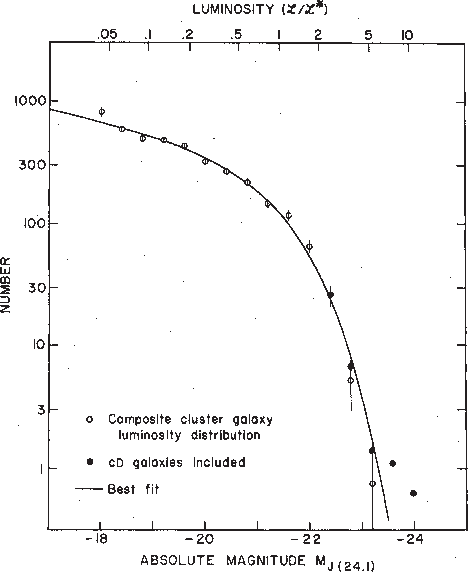
\includegraphics[width=0.4\textwidth]{schechter76}
    \caption{Fonction de luminosité des galaxies dans les amas d'Abell
      (Schechter, 1976).} 
    \label{schechter76}
  \end{SCfigure}
\end{Exercise}

\begin{Answer}
  \begin{enumerate}
  \item Cette fonction empirique montre bien la prédominance des
    galaxies de faible luminosité intrinsèque. Noter que le nombre
    total de galaxies $N_{T} = \int_{0}^{\infty} \Phi(L)\,\d L =
    \Phi^{*}\Gamma(\alpha+1)$ diverge pour $\alpha \leq -1$, mais que
    la luminosité totale $L_{T} = \int_{0}^{\infty} L\Phi(L)\,\d L =
    \Phi^{*}L^{*}\Gamma(\alpha+2)$ reste finie.
  \item On a $\Phi(L)\,\d L = \Phi(M)\,\d M$ avec $M - M^{*} = -2,5\log
    L/L^{*}$, d'où:
    $$
    \Phi(M) = 0,4 \ln 10\times \Phi^{*}\,10^{-0,4(\alpha
      +1)(M-M^{*})}\exp \left( -10^{-0,4(M-M^{*})} \right)
    $$
  \end{enumerate}

  \begin{SCfigure}[0.5]%[htp]
    \centering
    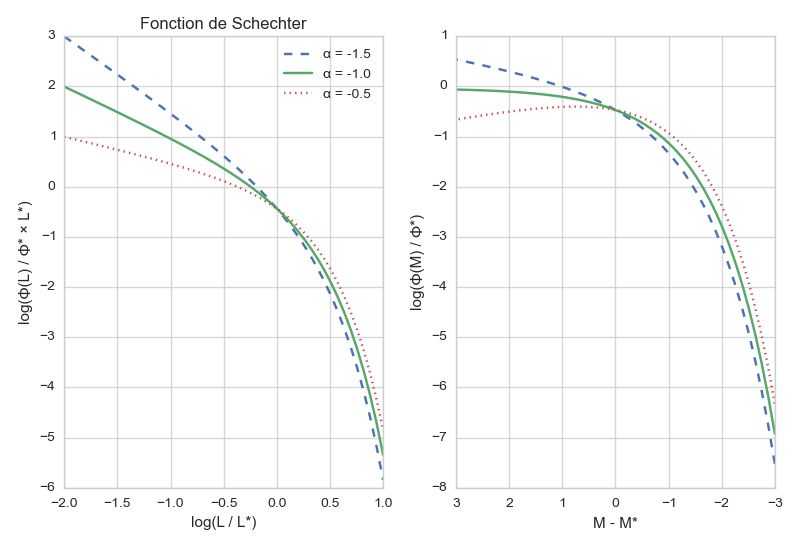
\includegraphics[width=0.6\textwidth]{schechter}
    \caption{Fonction (normalisée) de Schechter pour différentes
      valeurs de $\alpha$.}
    \label{schechter}
  \end{SCfigure}
\end{Answer}

%\subsubsection{Effets d'environnement, collisions et fusions}

\begin{Exercise}[Fréquence de collision dans un amas]
  On considère un amas de galaxies ayant les caractéristiques
  suivantes :
  \begin{itemize}
  \item il est supposé sphérique, de diamètre $D_{a}$,
  \item il contient $N_{g}$ galaxies identiques et réparties
    uniformément dans l'amas,
  \item les galaxies sont supposées animées d'une vitesse quadratique
    moyenne $v_{g}/\sqrt{2}$ (la vitesse \emph{relative} quadratique
    moyenne est donc $v_{g}$).
  \end{itemize}

  \begin{enumerate}
  \item Donner l'expression de la densité numérique de galaxies (le
    nombre par unité de volume) $n_{g}$ dans l'amas.

  \item On suppose que les galaxies ont un diamètre typique
    $d_{g}$. En modélisant les galaxies comme des sphères dures
    («~boules de billard~»), donner l'expression de la section
    efficace $S_{\mathrm{eff}}$ lors d'une interaction (collision)
    entre deux galaxies.

  \item Donner l'expression du nombre d'interactions que subit une
    galaxie de l'amas pendant un temps $\Delta t$. En déduire, pour
    une galaxie, le temps caractéristique de collision $\tau_{c}$ et
    le libre parcours moyen $\ell_{c}$.

  \item En déduire le temps $T_{c}$ entre deux interactions au sein de
    l'amas.

  \item Application numérique : considérons un amas avec $D_{a} =
    7$~Mpc, $N=850$ galaxies, $d_{g} = 20$~kpc et $v_{g} =
    650$~km/s. Explicitez le calcul numérique du temps moyen entre
    deux collisions pour cet amas.
  \end{enumerate}
\end{Exercise}

\begin{Answer}
  \begin{enumerate}
  \item Le volume de l'amas est $V_{a} = \pi D_{a}^3/6$ et la densité
    numérique de galaxies est donc $ n_{g} = N_{g}/V_{a} = 6N_{g}/\pi
    D_{a}^3$.

  \item Deux galaxies entreront en collision lorsqu'elle passent à une
    distance $< d_{g}$ l'une de l'autre. La section efficace de
    collision est donc l'aire du disque de rayon $d_{g}$ :
    $S_{\mathrm{eff}} = \pi d_{g}^{2}$.

  \item Considérons une galaxie. Le volume utile «~balayé~» par cette
    galaxie pendant le temps $\Delta t$ est $\Delta V = v_{g} \times
    S_{\mathrm{eff}} \times \Delta t$. Le nombre de collisions que
    subira cette galaxie pendant le temps $\Delta t$ est donc égal au
    nombre de galaxies dans le volume $\Delta V$ : $N_{c} = n_{g}
    \Delta V$. Le temps caractéristique de collision $\tau_{c}$
    correspond au $\Delta t$ tel que $N_{c} = 1$ ; le libre parcours
    moyen est $\ell_{c} = v_{g} \times \tau_{c}$:
    $$
    \tau_{c} = \frac{D_{a}^3}{6 N_{g} d_{g}^2 v_{g}}, 
    \qquad
    \ell_{c} = \frac{D_{a}^3}{6 N_{g} d_{g}^2}
    $$

  \item Application numérique : $v_{g} = 650\;\u{km/s} =
    665\;\u{kpc/Gan}$, $\tau_{c} = 253$~Gan, $T_{c} = \tau_{c}/N_{g} =
    297$~Man.
  \end{enumerate}
\end{Answer}


\subsection{Équilibre gravitationnel}

\begin{Exercise}[Théorème du Viriel scalaire]
  On considère le système Terre-Soleil. Le Soleil, de masse $\Msun$,
  est pris comme référence du mouvement ($v_\odot = 0$). On note
  $M_\oplus$ et $v_\oplus$ la masse et la vitesse de la Terre.
  \begin{enumerate}
  \item Écrire l'expression de l'energie cinétique du système
    Terre-Soleil.
  \item Énoncer le théorème du Viriel. En déduire l'expression de la
    distance $D$ d'équilibre entre la Terre et le Soleil. Faire
    l'application numérique, sachant que $\Msun = 2\e{30}$~kg,
    $M_\oplus = 5,97\e{24}$~kg et $v_\oplus = 30$~km/s.
  \item On considère un système d'étoiles binaires en équilibre. Pour
    simplifier, les étoiles sont prises de masses égales $M_{1} =
    M_{2} = \Msun$ et leurs vitesses sont considérées comme égales
    $v_1 = v_2 = v$.

    Expliciter la relation entre la distance entre ces deux étoiles et
    leur vitesse et calculer cette vitesse $v$ pour les distances
    d'équilibre $D$ suivantes : 1~UA, 10~UA et 100~UA.
  \end{enumerate}
\end{Exercise}

\begin{Answer}
  \begin{enumerate}
  \item $K = 1/2 M_\oplus v_\oplus^2$
  \item Théorème du Viriel : $2K + U = 0$ avec $U = -G\Msun
    M_\oplus/D$ d'où $D = G\Msun/v_\oplus^2 = 1$~UA.
  \item $K = 1/2\,M_{1}v_{1}^{2} + 1/2\,M_{2}v_{2}^{2} =
    \Msun v^{2} \stackrel{\mathrm{Viriel}}{=} -U/2 =
    +G\Msun^{2}/(2D)$ d'où $v = \sqrt{G \Msun/(2 D)}$, soit:
    \begin{center}
      \begin{tabular}{lccc}
        \toprule
        $D$ [UA]   & 1    & 10  & 100 \\
        \midrule
        $v$ [km/s] & 21,1 & 6,7 & 2,1 \\
        \bottomrule
      \end{tabular}
    \end{center}
  \end{enumerate}
\end{Answer}

\begin{Exercise}[Autres applications du théorème du Viriel]
  On va maintenant utiliser le théorème du Viriel pour remplir le
  tableau ci-dessous, donnant les rayons, masses et vitesse
  caractéristiques de différents système stellaires.  
  \begin{center}
    \begin{tabular}{lrrr}
      \toprule
      Système & $R$ & $V$ [km/s] & $M/\Msun$ \\ 
      \midrule
      Amas globulaire  & 10~pc  & 10   & \corrige{$4,6\e{5}$} \\ 
      Galaxie          & 15~kpc & 200  & \corrige{$2,8\e{11}$} \\ 
      Amas de galaxies & 1~Mpc  & 1000 & \corrige{$4,6\e{14}$} \\ 
      \bottomrule
    \end{tabular}
  \end{center}
\end{Exercise}

\begin{Answer}
  On a $U = -GM^{2}/(2R)$ et $K=1/2\, MV^{2}$ d'où $M = 2RV^{2}/G$,
  avec $G = 6,67\e{-11}\;\u{m^{3}~kg^{-1}~s^{-2}} =
  4,302\e{-3}\;\u{km^{2}~s^{-2}~pc~\Msun^{-1}}$.
\end{Answer}

\begin{Exercise}[Temps cinématique]
  On va maintenant calculer le temps cinématique $t_c$ pour différents
  systèmes stellaires. 
  \begin{center}
    \begin{tabular}{lrrr}
      \toprule
      Système & $R$ & $M/\Msun$ & $t_c$ [ans] \\ 
      \midrule
      Amas ouvert      & 1~pc   & 500      & \corrige{$9,4\e{5}$} \\ 
      Amas globulaire  & 10~pc  & $10^5$   & \corrige{$2,1\e{6}$} \\ 
      Galaxie          & 15~kpc & $10^{11}$ & \corrige{$1,2\e{8}$} \\ 
      Amas de galaxies & 1~Mpc  & $10^{14}$ & \corrige{$2,1\e{9}$} \\
      \bottomrule
    \end{tabular}
  \end{center}
  Que remarquez-vous sur ces temps cinématiques pour les différents
  systèmes ?
\end{Exercise}

\begin{Answer}
  $t_{c} = R/V = \sqrt{2R^{3} / GM}$ avec $G =
  4,500\e{-15}$~\u{pc^{3}~\Msun^{-1}~an^{-2}}.

  Les temps cinématiques pour un amas ouvert et un amas globulaire ne
  sont pas vraiment différents malgré leurs tailles respectives très
  différentes.  De même entre une galaxie et un amas globulaire : il
  ne faut qu'environ 100$\times$ plus de temps à une étoile avec une
  vitesse typique pour traverser une grosse galaxies qu'un amas
  globulaire (bien sur les vitesses caractéristiques ne sont pas les
  mêmes pour ces deux systèmes).
\end{Answer}

% ==============================================================================

\chapter{Cosmologie}

\section{Espace et temps absolus}

\begin{Exercise}[La faiblesse de la force de gravitation]
  Marcel et Naomi ressentent l'un pour l'autre une certaine
  attirance...  Quelle part en revient tout bêtement à la force de
  gravitation universelle, lorsque leurs centres de gravité respectifs
  sont distants de 1 mètre ?  Quelle masse $m$, au même point de la
  Terre, présente un poids égal à cette force ?  Marcel pèse 700~N, et
  Naomi 580~N.  Le rayon de la Terre sera supposé égal à $R_{\oplus} =
  6370$~km, et la masse de la Terre est de $M_{\oplus} =
  5,97\e{24}$~kg.
\end{Exercise}

\begin{Answer}
  Il s'agit d'appliquer la formule de Newton deux fois pour trouver
  les masses respectives de Marcel et Naomi, puis une troisième fois
  pour calculer l'attraction qui s'exerce entre eux: $F_{MN} = G\,m_M
  m_N/d^2 = G\,m M_{\oplus}/R_{\oplus}^2$.  Pour Marcel,
  $P_{\mathrm{M}} = G M_{\mathrm{M}}M_{\oplus} / R_{\oplus}^2$ soit
  $M_{\mathrm{M}} = P_{\mathrm{M}}R_{\oplus}^2 / (G M_{\oplus}) =
  71,3~\u{kg}$. Pour Naomi, on peut utiliser le fait que
  $M_{\mathrm{N}}/M_{\mathrm{M}} = P_{\mathrm{N}} / P_{\mathrm{M}}$,
  puisque les deux personnes sont soumises au même champ de gravité,
  donc $M_{\mathrm{N}} = M_{\mathrm{M}}\times
  P_{\mathrm{N}}/P_{\mathrm{M}} = 71,3 \times 580/700 = 59,0~\u{kg}$
  d'où $F_{\mathrm{NM}} = 2,81\e{-7}~\u{N}.$ La masse qui présente un
  poids égal à cette valeur est de $m =
  F_{MN}R_{\oplus}^{2}/(GM_{\oplus}) = 2,86\e{-8}\;\u{kg} =
  \SI{28,6}{\micro g}$.

  L'attraction gravitationnelle est une force \emph{très faible},
  c'est même la plus faible des quatre forces fondamentales de
  l'Univers.
\end{Answer}

% \subsection{Problèmes de l'Univers de Newton}

% \begin{Exercise}[L'instabilité gravitationnelle]
%   Pourquoi Newton pense-t-il que ces trois hypothèses supplémentaires
%   permettraient, chacune, de «~sauver~» l'Univers de la catastrophe
%   gravitationnelle ?
% \end{Exercise}

% \begin{Answer}
%   \begin{itemize}
%   \item Si l'Univers est infini, tout point est entouré d'une
%     distribution de matière à symétrie sphérique, et restera donc
%     immobile.
%   \item Si l'Univers est en expansion, c'est qu'il n'est pas en train
%     de se contracter !
%   \item Si l'Univers est très jeune, il n'a pas encore eu le temps de
%     démarrer sa contraction gravitationnelle de façon sensible.
%   \end{itemize}
% \end{Answer}

% \begin{Exercise}[Le paradoxe d'Olbers]
%   En quoi le fait que l'Univers soit jeune et en expansion peut-il
%   permettre d'expliquer la noirceur du ciel nocturne ?
% \end{Exercise}

% \begin{Answer}
%   \begin{itemize}
%   \item Si l'Univers est jeune, du fait de la vitesse finie de
%     propagation de la lumière, celle qui provient des objets très
%     lointains n'a pas eu le temps de nous parvenir.
%   \item Si l'Univers est en expansion, la lumière qui nous parvient
%     des objets très lointains a été affaiblie par cette expansion
%     (ceci sera traité plus loin dans le cours), au point de ne pas
%     être détectable.
%   \end{itemize}
% \end{Answer}

\section{La rupture relativiste}

% \subsection{Vitesse de la lumière}

% \begin{Exercise}[La première mesure de $c$]
%   Si Roemer a fait le calcul (ce que l'on ignore, mais cela semble
%   assez probable), et en supposant qu'il utilisait la même valeur de
%   la distance Terre-Soleil que les astronomes d'aujourd'hui, quelle
%   valeur de $c$ a-t-il obtenue ?
% \end{Exercise}

% \begin{Answer}
%   Si la lumière met $8+8 = 16$~min pour traverser l'orbite de la
%   Terre, c'est à dire pour franchir une distance de 2~U.A., sa
%   vitesse est $c = 2 \times 1,49598\e{11} / ( 16 \times 60 ) =
%   3,11\e{8}$~m/s. Ceci suppose que la valeur de l'U.A. admise alors
%   était la même qu'aujourd'hui, ce qui n'est certainement pas exact
%   : en 1675, on n'avait pas encore très bien mesuré la distance de
%   la Terre au Soleil... La valeur de deux fois huit minutes est
%   elle-même approximative. Roemer aurait plutôt trouvé $2\e{8}$~m/s,
%   dit-on. La première détermination sérieuse de l'Unité Astronomique
%   est due à Cassini et Richer, en 1671. Il faudra attendre le XXe
%   siècle et les méthodes d'écho radar pour disposer de mesures très
%   précises de cette valeur.
% \end{Answer}

\subsection{Relativité générale}

\begin{Exercise}[L'équivalence gravité/accélération]
  Pour la Relativité Générale, gravitation et accélération sont
  équivalentes, mais cette équivalence n'est que \emph{locale}: aucune
  expérience de physique ne permet de distinguer les effets de l'une
  de ceux de l'autre, \emph{à condition} de se limiter à un «~petit~»
  domaine spatial.

  En reprenant l'expérience de pensée de l'«~ascenseur d'Einstein,~»
  pouvez-vous montrer qu'il est en effet facile de distinguer
  pesanteur et accélération par la fusée si on abandonne la localité.
\end{Exercise}

\begin{Answer}
  À grande échelle, le champ de gravité qui environne un corps massif
  reste en général discernable d'une accélération constante.  Par
  exemple, dans l'image de l'ascenseur d'Einstein, il ne faut pas que
  la cabine soit trop étendue.  Sinon, le parallélisme ou le
  non-parallélisme des forces sur des masses éloignées l'une de
  l'autre trahirait la «~vraie~» nature du champ.  Sur la
  Fig.~\ref{grav}, la cabine de gauche, supposée accélérée vers le
  haut (flèche bleue), produit des forces parallèles (flèches rouges)
  sur les deux masses-test.  La cabine de droite, immobile dans le
  champ de gravitation de la Terre, montre des forces convergentes
  vers le centre de la Terre (flèches vertes).  De même, le physicien
  pourrait mettre en évidence une dépendance de la force avec
  l'altitude dans le cas de droite.
  \begin{SCfigure}%[htp]
    \centering
    \includegraphics[width=0.4\textwidth]{grav}
    \caption{}
    \label{grav}
  \end{SCfigure}
\end{Answer}

\subsection{Les tests}

\begin{Exercise}[Le décalage gravitationnel vers le rouge]
  Une lampe spectrale émettant dans la raie H$\alpha$ ($\lambda_{0} =
  656,3$~nm) est utilisée pour communiquer à partir d'une capsule en
  orbite serrée autour d'une étoile à neutrons. Le rayon de l'orbite
  est $R=1000$~km, la masse de l'étoile de $M=1,5$~\u{\Msun}.  À
  quelle longueur d'onde $\lambda$ le vaisseau qui a lancé la capsule,
  et se tient prudemment à grande distance, doit-il rechercher les
  signaux ?

  Comparer cet effet gravitationnel au décalage par effet Doppler du
  signal de la sonde en orbite circulaire autour de l'étoile à
  neutrons.
\end{Exercise}

\begin{Answer}
  Le décalage gravitationnel subi à la distance $R$ d'un corps de
  masse $M$ s'écrit :
  \begin{align*}
    z_{G} &= \frac{GM}{c^2 R} = \frac{ 6,672\e{-11} \times 1,5 \times
      1,989\e{30} }{ 299792458^{2}\e{6} } = 2,216\e{-3} \\
    &= \frac{\lambda - \lambda_{0}}{\lambda_0}
  \end{align*}
  d'où $\lambda = (1+z_{G})\lambda_0 = 1,00221 \times 656,3 = 657,75$~nm.

  La vitesse de l'orbite circulaire de rayon $R$ autour d'une masse
  $M$ est donnée (dans l'approximation non-relativiste) par:
  $$
  v = \sqrt{\frac{GM}{R}} = 14112\;\u{km/s} \simeq 4,71\e{-2} \times c
  $$
  Le décalage par effet Doppler (dans la même approximation non
  relativiste) est donc $z_{D} = v/c = \sqrt{z_{G}} \gg z_{G}$.
\end{Answer}


\section{Le Big Bang}

\subsection{Film des débuts}

\begin{Exercise}[Nucléosynthèse primordiale ou non ?]
  Les éléments légers $\mathrm{H}$, ${}^{2}\mathrm{H}$,
  ${}^{3}\mathrm{H}$, ${}^{4}\mathrm{He}$, ${}^{7}\mathrm{Li}$ sont
  nés avec le Big Bang. Mais d'où proviennent tous les autres éléments
  «~lourds~», ceux qui entrent dans la composition des objets du
  quotidien ?
\end{Exercise}

\begin{Answer}
  Les chapitres traitant des modèles stellaires et de l'évolution
  stellaire nous fournissent la réponse :
  \begin{itemize}
  \item Jusqu'au ${}^{56}\mathrm{Fe}$, les noyaux sont produits par
    les étoiles.  La source d'énergie de celles-ci est d'origine
    thermonucléaire, et elles sont des usines à fabriquer, par fusion,
    des noyaux lourds à partir de noyaux plus légers.
  \item Au-delà, seules les explosions de supernovae atteignent des
    températures suffisantes (plusieurs $10^9$~K) pour pouvoir
    synthétiser les noyaux très lourds, jusqu'aux éléments
    transuraniens.
  \item Quelques noyaux particuliers (${}^{6}\mathrm{Li}$,
    ${}^{9}\mathrm{Be}$, ${}^{10}\mathrm{B}$) sont sans doute formés
    lors des collisions des rayons cosmiques avec la matière
    interstellaire.
  \end{itemize}
\end{Answer}

\subsection{Expansion de l'Univers...}

\begin{Exercise}[... limitée par \emph{c} ?]
  Plus une galaxie est éloignée de notre Voie Lactée, plus les
  astronomes lui trouvent une vitesse d'éloignement élevée. C'est
  l'expansion de l'Univers. Mais, quand la distance croît sans cesse,
  elle atteint un moment une valeur $d_c$ telle que :
  $$
  V = H_0 d_c > c
  $$
  Étonnant, non ?
\end{Exercise}

\begin{Answer}
  Il est interdit par la Relativité Générale de mesurer une vitesse
  égale ou supérieure à $c$ pour un objet de masse non nulle, comme
  une galaxie. Cependant, cette limite ne s'applique pas à l'expansion
  de l'Univers, où les objets (p.ex. les galaxies) sont immobiles dans
  un espace dont la géométrie s'étire. Les galaxies très lointaines
  voient effectivement leur vitesse apparente atteindre celle de la
  lumière, et disparaissent alors de l'Univers observable. Ceci
  n'enlève rien au fait qu'elles continuent à s'éloigner de nous à des
  vitesses supérieures à $c$.  Signalons que nos moyens d'observation
  actuels sont loin de nous permettre d'observer les objets qui
  s'approchent de cette limite.
\end{Answer}

\begin{Exercise}[... la même partout ?]
  La radiogalaxie 3C~171 (la 171e entrée dans le troisième catalogue
  de radiources établi par l'observatoire de Cambridge) est
  relativement lointaine; entraînée par l'expansion de l'Univers, elle
  présente une vitesse de fuite de 63\,000~km/s.

  Montrer que malgré cela, l'astronome Pr.~Snurp, qui a là-bas
  découvert l'expansion de l'Univers, comme Hubble l'a fait pour nous,
  a lui aussi trouvé une loi qui s'écrit :
  $$
  v_0 = X_0 d_{0},
  $$
  $v_0$ étant la vitesse mesurée à partir de 3C~171 pour une galaxie
  lointaine située à la distance $d_0$ de 3C~171, et que la constante
  de Snurp $X_0$ partage la valeur de $H_{0}$.

  Ainsi, d'une planète de 3C~171, comme de la Terre, on observe la même
  expansion universelle, avec la même géométrie, et le même taux...
\end{Exercise}

\begin{Answer}
  Désignons par $v_T$ et $d_T$ les vitesses et distances mesurées à
  partir de la Terre, $v_{3C}$ et $d_{3C}$ celles mesurées à partir de
  3C~171.  La vitesse de récession de 3C~171 mesurée de la Terre est
  donc $v_T(3C\;171) = 63\;000$~km/s.

  Considérons une autre galaxie, $G$, observée à la fois de la Terre
  et de 3C~171. On peut écrire :
  \begin{align*}
    \vec{v}_{3C}(G) &= \vec{v}_{3C}(T) + \vec{v}_{T}(G) \\
    &= -\vec{v}_{T}(3C\;171) + \vec{v}_{T}(G) \\
    &= -H_0\vec{d}_{T}(3C\;171) + H_0\vec{d}_{T}(G) \\
    &= H_0 \left[ \vec{d}_{T}(G) - \vec{d}_{T}(3C\;171) \right ] \\
    &= H_0 \vec{d}_{3C}(G)
  \end{align*}
  et donc, à partir de 3C~171 comme de la Terre, toute les galaxie
  observée semble s'enfuir avec une vitesse proportionnelle à sa
  distance, et le facteur de proportionnalité (la constante de Snurp)
  est universel : $X_0=H_0$ (Fig.~\ref{H0}).

  \begin{SCfigure}%[htp]
    \centering
    \includegraphics[width=0.4\textwidth]{351922_281}
    \caption{}
    \label{H0}
  \end{SCfigure}
\end{Answer}

\subsection{Constante de Hubble \& Co.}

Dans les exercices suivants, on supposera la constante de Hubble égale
à $H_0 = 70$~\u{km~s^{-1}~Mpc^{-1}}.

\begin{Exercise}[Le facteur d'expansion de l'espace]
  La constant de Hubble $H_0$ est usuellement exprimée en kilomètres
  par seconde et par mégaparsec, mais cela ne parle guère au sens
  commun.  Quelle est la valeur de l'accroissement annuel d'un
  kilomètre ?
\end{Exercise}

\begin{Answer}
  $1\;\u{Mpc} = 3,09\e{19}\;\u{km}$ et $1\;\u{an} = 3,16\e7\;\u{s}$,
  donc $71\;\u{km~s^{-1}~Mpc^{-1}} = 2,27\e{-18}\;\u{km~s^{-1}~km^{-1}}
  = 71,6\;\u{nm~an^{-1}~km^{-1}}$.
\end{Answer}

\begin{Exercise}[Temps de Hubble]
  Calculez le temps de Hubble $t_{H} = 1/H_{0}$. Quelle est sa
  signification physique ?  Quelle conclusion pouvez-vous en tirer sur
  l'âge de l'Univers ?
\end{Exercise}

\begin{Answer}
  Le temps de Hubble est défini par $1/t_{H} = H_0 =
  70\;\u{km~s^{-1}~Mpc^{-1}} = 2,27\e{-18}\;\u{s^{-1}}$ d'où $t_{H} =
  4,41\e{17}~s \simeq 13,97\e{9}$~ans. Il représente l'âge de
  l'Univers dans le cas d'un taux d'expansion \emph{constant}. On peut
  donc penser que l'Univers est âgé d'environ 14~Gans.
\end{Answer}

\begin{Exercise}[Densité critique]
  Calculer la densité critique $\rho_{C} = \dfrac{3 H_{0}^{2}}{8\pi G}$.
  Quelle est sa dimension ?  La convertir en nucléons/$\u{m^{3}}$ ($m_{p}
  \simeq m_{n} \simeq m_{u} = 1,66\e{-27}$~kg), puis en $\Msun/\u{Mpc}^{3}$.
  Commenter.
\end{Exercise}

\begin{Answer}
  $\rho_{C} = 9,20\e{-27}~\u{kg\;m^{-3}} = 5,54\;\text{nucléons}\;\u{m^{-3}} =
  1,34\e{11}\;\Msun\;\u{M\pc}^{-3}$, soit environ une galaxie (massive) par
  \u{M\pc^{3}}, densité caractéristique de l'Univers local.
\end{Answer}

\begin{Exercise}[Âge de l'Univers]
  À partir de la définition de $H_0$ et de la relation $R \propto
  t^{2/3}$ entre le facteur d'échelle $R$ et le temps $t$ dans le cas
  d'un Univers euclidien ($k=0$) dominé par la matière
  ($\Omega_{M}=1$, $\Omega_{\Lambda}=0$), trouver la relation entre
  $H_{0}$ et $t$.
\end{Exercise}

\begin{Answer}
  \begin{align*}
    H_0 &\defeq \frac{1}{R}\frac{\d R}{\d t} \\
    &= \left ( \frac{t}{t_0} \right )^{-2/3} \times
    \frac{\d\left( t/t_0 \right )^{2/3}}{\d t} 
    = \left ( \frac{t}{t_0} \right )^{-2/3} \times
    \left( \frac{t}{t_0} \right)^{-1/3} \frac{2}{3} \frac{1}{t_0} 
    = \left( \frac{t}{t_0} \right)^{-1} \times \frac{2}{3t_0} \\
    &= \frac{2}{3t} \\
    \text{donc}\quad t &= \frac{2}{3\,H_{0}}
  \end{align*}
  Pour un Univers critique dominé par la matière, l'âge de l'Univers
  est égal aux deux-tiers du temps de Hubble.
\end{Answer}

\section{Modèles cosmologiques}

\begin{Exercise}[Modèle FLRW]
  Dans le cas d'un Univers de Friedmann-Lemaître-Robertson-Walker à
  courbure spatiale nulle ($k=0$), on a :
  \begin{equation}
    \left(\frac{\dot{R}}{R}\right)^{2} = 
    \frac{\Lambda}{3} + \frac{8\pi G}{3}\rho.
    \label{eq:1}
  \end{equation}
  Par ailleurs, l'équation de conservation de l'énergie s'écrit
  toujours:
  \begin{equation}
    \label{eq:2}
    \dot{\rho} = -3\left(\rho + \frac{P}{c^{2}}\right)\frac{\dot{R}}{R}.
  \end{equation}

  \begin{enumerate}
  \item Que signifient les différents termes -- $R$, $\Lambda$, $\rho$
    -- de l'équation~(\ref{eq:1}) ? Quelle est la dimension de
    $\dot{R}/R$ ?  Comment s'appelle cette quantité ?

  \item Si l'on considère le fluide parfait dont l'équation d'état --
    reliant la pression $P$ à la densité $\rho$ -- est donnée par $P =
    w\rho c^{2}$, que devient l'équation~(\ref{eq:2}) ? Vérifier que
    l'on obtient alors, en notant $\rho(R_{0}) = \rho_{0}$ :
    $$
    \frac{\rho}{\rho_{0}} = \left(\frac{R}{R_{0}}\right)^{-3(1+w)}.
    $$

  \item Dans le cas où $\Lambda = 0$, en déduire que $R$ est régit par
    une équation différentielle du type :
    $$
    \dot{R} = \alpha R^{-\eta},
    $$
    avec $\eta = (1+3w)/2$. Expliciter la valeur de $\alpha$.

  \item On peut montrer que la solution générale de l'équation
    différentielle précédente est de la forme :
    $$
    \frac{R}{R_{0}} = \left(\frac{t}{t_{0}}\right)^{\gamma}.
    $$
    Déterminer $\gamma$ en fonction de $\eta$, puis de $w$.

  \item Exprimer alors $\dot{R}/R$ en fonction de $t$.

  \item Dans le cas d'un Univers dominé par la matière ($w=0$),
    comment est relié l'âge de l'Univers $t_{0}$ à la constante de
    Hubble $H_{0}$ ? Même question dans le cas d'un univers dominé par
    les radiations ($w=1/3$).
  \end{enumerate}
\end{Exercise}

\begin{Answer}
  \begin{enumerate}
  \item $R$ : facteur d'échelle, $\Lambda$ : constante cosmologique,
    $\rho$ : densité massique.  $\dot{R}/R$ a la dimension de
    l'inverse d'un temps, c'est la constante de Hubble $H$.

  \item $\dot{\rho} = -3(1+w) H$. On vérifie que $\rho/\rho_{0} =
    (R/R_{0})^{-3(1+w)}$ est bien solution de cette équation.

  \item En introduisant la solution précédente dans
    l'éq.~(\ref{eq:1}), on obtient $\dot{R} = \alpha R^{-\eta}$ avec
    $$
    \alpha = 
    \left( \frac{8\pi G}{3}\rho_{0}R_{0}^{3(1+w)} \right)^{1/2}
    \qquad\text{et}\qquad \eta = \frac{1+3w}{2}
    $$

  \item En égalisant les expressions de $\dot{R}$, on obtient
    $$
    \gamma = \frac{1}{1+\eta} = \frac{2}{3(1+w)}.
    $$

  \item On a
    $$
    H = \frac{\dot{R}}{R} = \frac{\gamma}{t} =
    \frac{2}{3(1+w)}\frac{1}{t}.
    $$

  \item Pour $w=0$, $t_{0} = 2/(3 H_{0})$ ; pour $w=1/3$, $t_{0} =
    1/(2 H_{0})$.
  \end{enumerate}
\end{Answer}

\begin{Exercise}[\emph{Redshift} cosmologique]
  La radiogalaxie 4C~41.17 montre une raie spectrale intense à
  582,2~nm.  Cette raie est identifiée comme la raie Lyman~$\alpha$ de
  l'hydrogène. En laboratoire, sur la Terre, la longueur d'onde de
  cette raie est de 121,5~nm.

  \begin{enumerate}
  \item Quel est le redshift de la radiogalaxie 4C~41.17 ?
  \item Quel était le facteur d'échelle de l'Univers à l'époque où les
    atomes d'hydrogène de 4C~41.17 émettaient cette raie ?
  \item À quelle époque $t_{em}$ la radiogalaxie 4C~41.17 de
    l'exercice précédent a-t-elle émis la lumière que nous recevons
    aujourd'hui à $t_0$ ? On supposera un Univers critique dominé par
    la matière, avec un âge de $t_0 = 13,5\e9$~ans.
  \end{enumerate}
\end{Exercise}

\begin{Answer}
  \begin{enumerate}
  \item $1 + z = \lambda_{\text{observé}}/\lambda_{\text{émis}} =
    582,2/121,5 = 4,792$ donc $z = 3,792$.
  \item Par ailleurs, $1 + z =
    \lambda_{\text{observé}}/\lambda_{\text{émis}} =
    R_0/R_{\text{émission}}$, soit $R_{e}/R_{0} = \lambda_{0}/\lambda
    = 121,5/582,2 = 0,209$.  À l'époque où 4C~41.17 émettait la
    lumière qui nous parvient aujourd'hui, l'Univers était cinq fois
    moins «~étiré~» qu'aujourd'hui.
  \item Pour un Univers critique dominé par la matière, $R(t)/R_{0} =
    (t/t_0)^{2/3}$, et donc $t_{e} = t_0 \times
    \left(R_{em}/R_{0}\right)^{3/2}$, soit $t_{e} = 13,5 \times
    0,209^{3/2} = 1,29\e{9}$~années.  4C~41.17 émettait la lumière qui
    nous parvient aujourd'hui alors que l'Univers n'était âgé que de
    1,29 milliards d'années.
  \end{enumerate}
\end{Answer}

\begin{Exercise}[Temps de vol, distance, et expansion...]
  Il y a dix milliards d'années, ce photon que nous recevons
  aujourd'hui a quitté une lointaine galaxie.
  \begin{enumerate}
  \item Cette galaxie se trouvait-elle à dix milliards
    d'années-lumière de nous au moment de l'émission ?
  \item Cette galaxie se trouve-t-elle aujourd'hui à dix milliards
    d'années-lumière de nous ?
  \end{enumerate}
\end{Exercise}

\begin{Answer}
  \begin{enumerate}
  \item Le photon a voyagé pendant dix milliards d'années en luttant
    contre l'expansion de l'espace qui contrariait son mouvement; tout
    se passe comme s'il avait parcouru à la vitesse $c$ une distance
    supérieure à celle qui séparait la galaxie de nous au moment de
    l'émission.  Au moment de l'émission, la galaxie était donc à
    moins de dix milliards d'années-lumière de nous.
  \item Depuis que le photon a quitté la galaxie, celle-ci, entraînée
    par l'expansion, a continué à s'éloigner de nous. Le photon a bien
    parcouru (de son point de vue, en admettant qu'il en ait un) dix
    milliards d'années-lumière, puisque sa vitesse par rapport à
    l'espace est à tout instant égale à $c$, mais la galaxie a
    continué sa route pendant tout ce temps, et se trouve aujourd'hui
    à plus de dix milliards d'années-lumière de nous...
  \end{enumerate}
\end{Answer}

% ==============================================================================

\chapter{Retour sur Terre: nos repères dans le ciel}

\section{Se positionner dans le ciel}

\begin{Exercise}[Repérage]
  \begin{enumerate}
  \item Quelles sont les coordonnées horizontales des quatre points
    cardinaux ?

  \item Peut-on définir les coordonnées horizontales pour un
    observateur installé au pôle Nord géographique ou au pôle Sud ?

  \item Pour quelles valeurs de la hauteur et de la distance zénithale
    un astre est-il visible, c'est-à-dire au dessus de l'horizon ?
  \end{enumerate}
\end{Exercise}

\begin{Answer}
  \begin{enumerate}
  \item Les points cardinaux étant par définition sur l'horizon, leurs
    hauteurs sont nulles. Les directions Est-Ouest et Nord-Sud étant
    orthogonales, on a à partir de l'origine la direction Sud
    (Fig.~\ref{position}) :
    \begin{center}
      \begin{tabular}{lrr}
        \toprule
        & Azimut & Hauteur \\ 
        \cmidrule(r){2-3}
        Nord  & 180° & 0 \\ 
        Est   & 270° & 0 \\ 
        Sud   & 0°   & 0 \\ 
        Ouest & 90°  & 0 \\ 
        \bottomrule
      \end{tabular}
    \end{center}
    Remarque : L'azimut des marins est décalé de 180° par rapport à
    celui des astronomes. L'origine des azimuts est le Nord.

  \item Seule la hauteur d'un astre au-dessus de l'horizon peut être
    définie. L'azimut ne l'est pas, la ligne Nord-Sud ou le plan
    méridien étant indéterminé. La verticale du lieu est confondue
    avec l'axe de rotation de la Terre et tout plan passant par la
    verticale du pôle répond à la définition du plan méridien.

  \item Un astre n'est visible que s'il est au-dessus de l'horizon. Sa
    hauteur doit être positive par définition. Sa distance zénithale
    ($90\deg - h$) par conséquent est plus petite que 90°.  Un astre
    sous l'horizon a sa distance zénithale plus grande que 90°
    (Fig.~\ref{position2}).
  \end{enumerate}

  \begin{figure}
    \centering
    \begin{subfigure}[b]{0.4\textwidth}
      \centering
      \includegraphics[width=\textwidth]{position}
      \caption{Points cardinaux.}
      \label{position}
    \end{subfigure}
    \begin{subfigure}[b]{0.4\textwidth}
      \centering
      \includegraphics[width=\textwidth]{position2}
      \caption{Horizon et distance zénithale.}
      \label{position2}
    \end{subfigure}
    \caption{}
  \end{figure}
\end{Answer}

\section{Mouvement diurne}

\begin{Exercise}
  \begin{enumerate}
  \item Dans quelle direction se trouve un astre au moment de sa
    culmination en un lieu de latitude $+50\deg$ ?
  \item Même question pour un lieu situé à l'équateur.
  \item La hauteur d'un astre varie-t-elle au cours du mouvement
    diurne au pôle Nord ?
  \end{enumerate}
\end{Exercise}

\begin{Answer}
  \begin{enumerate}
  \item Lors du mouvement diurne, la culmination d'un astre se produit
    lorsque sa hauteur est maximale.  Suivant sa position de l'objet
    sur la sphère céleste (donc sa déclinaison), l'astre passera entre
    le zénith et le pôle (Nord pour un habitant de l'hémisphère nord
    et Sud pour...) soit entre le zénith et l'horizon opposé au pôle
    visible. À la latitude de 50°, les étoiles dont la déclinaison est
    plus petite que la latitude, la culmination se fera du côté Sud de
    l'observateur.  Pour les autres étoiles, la culmination sera du
    côté Nord (Fig.~\ref{mouvementdiurne2})

    \begin{figure}
      \centering
      \begin{subfigure}[b]{0.3\textwidth}
        \centering
        \includegraphics[width=\textwidth]{mouvement_diurne2}
        \caption{Latitude $\phi\sim 50\deg$.}
        \label{mouvementdiurne2}
      \end{subfigure}
      \begin{subfigure}[b]{0.3\textwidth}
        \centering
        \includegraphics[width=\textwidth]{mouvement_diurne3}
        \caption{Équateur ($\phi = 0$).}
        \label{mouvementdiurne3}
      \end{subfigure}
      \begin{subfigure}[b]{0.3\textwidth}
        \centering
        \includegraphics[width=\textwidth]{mouvement_diurne4}
        \caption{Pôle nord ($\phi = 90\deg$.}
        \label{mouvementdiurne4}
      \end{subfigure}
      \caption{Mouvement diurne.}
    \end{figure}

  \item L'équateur passant par le zénith, toutes les étoiles de
    déclinaisons positives culminent au Nord et les étoiles de
    déclinaisons négatives au Sud. Les étoiles de déclinaisons nulles
    passent au zénith (Fig.~\ref{mouvementdiurne3}).

  \item La verticale étant confondue avec l'axe du pôle, et l'horizon
    avec l'équateur, la déclinaison est égale à la hauteur de l'astre
    qui reste constante lors de la rotation diurne.  Seuls les objets
    de déclinaisons positives sont visibles. C'est pourquoi le Soleil
    dans son mouvement apparent durant l'année donne 6 mois
    consécutifs de jour et 6 mois consécutifs de nuit
    (Fig.~\ref{mouvementdiurne4}).
  \end{enumerate}
\end{Answer}

\begin{Exercise}[Mouvement diurne]
  \begin{enumerate}
  \item Comment varie l'azimut d'un astre au cours du mouvement
    diurne, en un lieu de latitude $+50\deg$ ? Et aussi $-50\deg$ de
    latitude. Sur la Fig.~\ref{mouvementdiurne}, on a représenté la
    situation en un lieu de l'hémisphère Sud (latitude = $-50\deg$) ;
    $P$ est alors en-dessous de l'horizon et $P'$ est au-dessus.

    \begin{SCfigure}[0.5]%[htp]
      \centering
      \includegraphics[width=0.5\textwidth]{mouvement_diurne}
      \caption{Rotation d'une étoile vue de l'hémisphère sud (latitude =
        $-50\deg$).}
      \label{mouvementdiurne}
    \end{SCfigure}

  \item Les astres se lèvent-ils du côté de l'Est et se couchent-ils
    du côté de l'Ouest aussi bien dans l'hémisphère Nord que dans
    l'hémisphère Sud ?
  \item Dans quelle direction géographique un astre culmine-t-il en un
    lieu de latitude $-50\deg$ ?
  \item Le mouvement diurne est-il observé dans le même sens pour un
    observateur de l'hémisphère Nord ou un observateur de l'hémisphère
    Sud ?
  \end{enumerate}
\end{Exercise}

\begin{Answer}
  \begin{enumerate}
  \item
    \begin{description}
    \item[Observateur de l'hémisphère Nord (latitude $+50\deg$)] On
      n'envisagera que le cas des étoiles visibles par l'observateur,
      c'est-à-dire celles dont $\delta > -(\pi/2 - \phi)$. Deux
      critères sont a envisager :
      \begin{itemize}
      \item l'étoile a une déclinaison plus grande que la latitude
        $\delta>\phi$ ou $\delta<\phi$
      \item l'étoile est circumpolaire $\delta > \pi/2 - \phi$
      \end{itemize}
      Par la première condition, si $\delta<\phi$, l'azimut de
      l'étoile varie de 0 à 360°, sinon, son azimut oscille entre une
      valeur comprise $\alpha$ entre 90 et 180° suivant sa position au
      passage au méridien et $360\deg-\alpha$. L'étoile oscille donc
      entre $\alpha$, 180° et $360\deg-\alpha$.

      Le deuxième critère (circumpolarité) indique si l'étoile a un
      lever ou un coucher, son azimut varie alors entre les positions
      des levers et couchers et celles définies par le premier
      critère.

      L'observateur orienté vers le Nord voit tourner les étoiles dans
      le sens direct autour du pôle Nord.

    \item[Observateur de l'hémisphère Sud (latitude $-50\deg$)] Les
      mêmes critères s'appliquent pour les limitations des azimuts et
      des levers et couchers, à la différence que l'azimut va osciller
      autour de la valeur 0° et que regardant le pôle Sud, il verra
      tourner les étoiles dans le sens rétrograde
      (Fig.~\ref{mouvementdiurne}).
    \end{description}
  \item Oui. Que l'on soit dans l'hémisphère Nord ou Sud, le sens de
    rotation de la Terre est le même. Les objets apparaissent à l'Est
    et se couchent à l'Ouest.

  \item Au Nord si sa déclinaison est plus grande que la latitude,
    autrement au Sud (Voir exercice 1 du même chapitre).

  \item Non (Voir exercice 4 du chapitre II).
  \end{enumerate}
\end{Answer}

\begin{Exercise}[Coordonnées horaires]
  \begin{enumerate}
  \item Quelle est la relation entre la déclinaison et la distance
    polaire d'un astre ?
  \item Quelles sont les coordonnées horaires des quatre points
    cardinaux en un lieu de latitude $\phi$ ?
  \item Que vaut la déclinaison du zénith en fonction de la latitude
    du lieu ?
  \end{enumerate}
\end{Exercise}

\begin{Answer}
  \begin{enumerate}
  \item Comme son nom l'indique, la distance polaire est l'angle entre
    la direction du pôle nord et la direction de l'objet, donc
    $p=90\deg-\delta$

  \item Table~\ref{tbl:coordonneeshoraires} et
    Fig.~\ref{fig:coordonneeshoraires}

    \begin{center}
      \begin{tabular}{lrc}
        \toprule
        & Angle horaire & Déclinaison \\ 
        \cmidrule(r){2-3}
        Sud   & 0~h  & $\phi - 90\deg$ \\ 
        Ouest & 6~h  & 0 \\ 
        Nord  & 12~h & $90\deg - \phi$ \\ 
        Est   & 18~h & 0 \\ 
        \bottomrule
      \end{tabular}
      \label{tbl:coordonneeshoraires}
    \end{center}

    \begin{figure}
      \centering
      \begin{subfigure}[b]{0.45\textwidth}
        \centering
        \includegraphics[width=\textwidth]{coordonnees_horaire}
        \caption{Points cardinaux.}
        \label{fig:coordonneeshoraires}
      \end{subfigure}
      \begin{subfigure}[b]{0.45\textwidth}
        \centering
        \includegraphics[width=\textwidth]{coordonnees_horaire2}
        \caption{Zénith.}
        \label{fig:coordonneeshoraires2}
      \end{subfigure}
      \caption{Coordonnées horaires.}
    \end{figure}

  \item La déclinaison du zénith vaut la latitude (positive pour
    l'hémisphère Nord et négative pour l'hémisphère Sud), voir
    Fig.~\ref{fig:coordonneeshoraires2}.
  \end{enumerate}
\end{Answer}

\begin{Exercise}[Coordonnées équatoriales]
  \begin{enumerate}
  \item Une étoile traverse le méridien sud à une hauteur de 85°, et
    le méridien nord à 45°. Trouver la déclinaison de l'étoile et la
    latitude de l'observateur.
  \item Où ces affirmations sont-elles vraies ?
    \begin{enumerate}
    \item Castor ($\alpha$-Gem, déclinaison $+31\deg54'$) est
      circumpolaire.
    \item Bételgeuse ($\alpha$-Ori, $7\deg24'$) culmine au
      zénith.
    \item $\alpha$-Cen ($-60\deg46'$) s'élève à une hauteur de 20° au
      méridien.
    \end{enumerate}
  \end{enumerate}
\end{Exercise}

\begin{Answer}
  \begin{enumerate}
  \item L'étoile tournant autour de la direction du pôle, les deux
    directions $OA$ et $OB$ des passages supérieur et inférieur, sont
    symétriques par rapport à l'axe $OP$. L'angle $\alpha$ égale
    l'angle $\beta$ et
    $$
    \alpha + \beta+180\deg - 45\deg -85\deg = 50\deg
    \quad\text{donc}\quad
    \alpha=\beta=25\deg
    $$
    $\alpha$ et $\beta$ sont tous deux les compléments de la
    déclinaison de l'étoile :
    $$
    \beta+\delta = 90\deg
    \quad\text{donc}\quad
    \delta=65\deg
    $$
    On calcule la latitude qui vaut la hauteur du pôle au dessus de
    l'horizon : $\phi = \alpha+45\deg = 70\deg$.

    \begin{SCfigure}%[htp]
      \centering
      \includegraphics[width=0.5\textwidth]{coordonnees_horaire3}
      \caption{Coordonnées horaires.}
      \label{fig:coordonneeshoraires3}
    \end{SCfigure}

  \item
    \begin{description}
    \item[Castor (Gem, $\delta = +31\deg56'$) circumpolaire:]
      L'étoile sera juste circumpolaire, c'est-à-dire passera tangent
      à l'horizon Nord, si sa déclinaison est le complément de la
      latitude.  Pour toute latitude plus grande, l'étoile sera plus
      élevée sur l'horizon et ne disparaîtra pas derrière celui-ci
      (Fig \ref{castor}) : $\phi>=90\deg-\delta$
      \begin{figure}[htp]
        \centering
        \begin{subfigure}[b]{0.3\textwidth}
          \centering
          \includegraphics[width=\textwidth]{castor}
          \caption{Castor.}
        \label{castor}
        \end{subfigure}
        \begin{subfigure}[b]{0.3\textwidth}
          \centering
          \includegraphics[width=\textwidth]{betelgeuse}
          \caption{Bételgeuse.}
          \label{betelgeuse}
        \end{subfigure}
        \begin{subfigure}[b]{0.3\textwidth}
          \centering
          \includegraphics[width=\textwidth]{cen}
          \caption{$\alpha$-Cen.}
          \label{cen}
        \end{subfigure}
        \caption{Coordonnées équatoriales.}
      \end{figure}

    \item[Bételgeuse (Ori, $\delta = +7\deg24'$) culmine au zénith:]
      Si l'étoile est au moment de sa culmination au zénith
      (nécessairement), sa déclinaison est égale à la latitude
      (Fig.~\ref{betelgeuse}) : $\phi=7\deg24'$

    \item[$\alpha$-Cen ($\delta = - 60\deg46'$) s'élève à une hauteur
      de +20°:] À son passage supérieur, l'étoile se trouve dans la
      configuration Fig.~\ref{cen}.  La latitude est l'angle $PON$ qui
      est égal à $P'OS$. En appliquant la relation de Chasles entre
      $P'OS$ la hauteur de l'astre 20° et la déclinaison, on obtient :
      $P'OS = 90\deg + \delta - 20\deg$ d'où $\phi = 9\deg14'$
    \end{description}
  \end{enumerate}
\end{Answer}

\section{Mouvement du Soleil}

\subsection{Année sidérale, année tropique }

\begin{Exercise}[Mouvement du Soleil, jour solaire]
  \begin{enumerate}
  \item Que valent la hauteur maximale et la hauteur minimale du
    Soleil en chacun des lieux considérés : 50°, 75°, 10°, 20° ?

  \item À quelle condition doit satisfaire la latitude d'un lieu pour
    que le Soleil n'ait ni lever ni coucher ?

  \item Comment comprendre l'expression «~soleil de minuit~» ?

  \item À quelle condition doit satisfaire la latitude d'un lieu pour
    que le Soleil puisse passer à son zénith ?

  \item Comment comprendre l'expression «~tropique du Cancer~» et «
    tropique du Capricorne~» ? on pourra discuter cette question, en
    particulier, en consultant une carte céleste.
  \end{enumerate}
\end{Exercise}

\begin{Answer}
  \begin{enumerate}
  \item Inclinaison de l'écliptique sur l'équateur :
    $\epsilon=23\deg27'$. On détermine les relations qui relient la
    latitude $\phi$, les hauteurs minimum et maximum avec les deux
    positions du Soleil en déclinaison $\pm \epsilon$.
    \begin{itemize}
    \item Position solstice hiver : $SOm = SOE - \epsilon =
      (90\deg-\phi) -\epsilon$
    \item Position solstice été : $SOm = SOE + \epsilon =
      (90\deg-\phi) +\epsilon$
    \end{itemize}
    ou le supplément si le Soleil sous les tropiques est passé de
    l'autre côté.
    \begin{center}
      \begin{tabular}{lcccc}
        \toprule
        Latitude $\epsilon$ & 50° & 75° & 10° & $-$20° \\
        Hauteur max. & $63\deg27'$ & $38\deg27'$ & $90\deg$ & $90\deg$ \\
        Hauteur min. & $16\deg33'$ & $-08\deg27'$ & $56\deg33'$ & $46\deg33'$ \\
        \bottomrule
      \end{tabular}
    \end{center}
    Attention aux positions entre les tropiques, le Soleil au solstice
    d'été pour les latitudes nord (solstice d'hiver pour les latitudes
    sud) est passé au Sud (au Nord) et de ce fait est plus bas que le
    jour où il passe au zénith au méridien (Fig.~\ref{mvtsolaire}).

    \begin{figure}
      \centering
      \begin{subfigure}[b]{0.45\textwidth}
        \centering
        \includegraphics[width=\textwidth]{mvt_soleil}
        \caption{}
        \label{mvtsolaire}
      \end{subfigure}
      \begin{subfigure}[b]{0.45\textwidth}
        \centering
        \includegraphics[width=\textwidth]{mvt_soleil2}
        \caption{}
        \label{mvtsolaire2}
      \end{subfigure}
      \caption{}
    \end{figure}

  \item Ceci se produit dans l'hémisphère nord en été quand le Soleil
    a une déclinaison suffisamment positive. On appelle ce phénomène
    le «~soleil de minuit~». Sur la figure ci-contre (cas de
    l'hémisphère Nord), lorsque au passage inférieur, l'angle $NOD$
    est positif, le Soleil ne se couche pas, son mouvement est
    circumpolaire.
    \begin{align*}
      NOD = NOE' + E'OD &> 0 \\
      90\deg - \phi &< \delta_{\odot} \\
      \phi &> 90\deg - \delta_{\odot}
    \end{align*}
    Au jour des solstices ($\delta_{\odot} = \pm 23\deg27'$) il
    suffit d'être à une latitude $\phi > 66\deg33'$ (en été pour
    l'hémisphère Nord) ou $\phi < - 66\deg33'$ (en hiver pour
    l'hémisphère Sud) ; les lieux de latitude $\phi$ égale à $\pm
    66\deg33'$ définissent sur le globe terrestre les parallèles
    appelés «~cercles polaires~» (respectivement boréal et austral)
    (Fig.~\ref{mvtsolaire2}).

  \item Vers les pôles, lors de son passage inférieur dans le plan
    méridien, le Soleil est au-dessus de l'horizon et son angle
    horaire ayant augmenté de 180° depuis sa culmination (par
    définition, il s'agit alors de «~midi~», 0~h temps solaire) vaut
    12~h, cela correspond bien à «~minuit~». À noter que le Soleil de
    minuit s'observe au Nord dans l'hémisphère boréal et au Sud dans
    l'hémisphère Sud.

  \item Pour que le Soleil passe au zénith, il faut que la déclinaison
    du zénith (qui est aussi la latitude du lieu) soit égale à celle
    du Soleil; comme cette dernière ne peut varier qu'entre
    $+23\deg27'$ et $-23\deg27'$, les lieux en question sont ceux
    de latitude comprise entre $-23\deg27'$ et $+23\deg27'$. Le
    Soleil passe au zénith de ces lieux deux fois dans le cours d'une
    année, au printemps et en été dans l'hémisphère Nord et en automne
    et en hiver dans l'hémisphère Sud. Les zones de la Terre qui
    correspondent à cette propriétés sont appelées les zones
    tropicales car situées entre le tropique nord du Cancer et le
    tropique sud du Capricorne.

  \item Pour les lieux de latitude égale à $+23\deg27'$ et
    $-23\deg27'$, le Soleil passe au zénith au moment des
    solstices. Ces lieux définissent sur le globe terrestre les
    parallèles appelés «~tropiques~» (du Cancer pour l'hémisphère Nord
    et du Capricorne pour l'hémisphère Sud). Si l'on se reporte à une
    carte du ciel, on voit qu'au moment des solstices le Soleil se
    trouve dans la direction de la constellation des Gémeaux (été) ou
    du Sagittaire (hiver). Il faudrait donc désigner les lieux en
    question par les noms : «~tropique des Gémeaux~» au lieu de
    tropique du Cancer et de même «~tropique du Sagittaire~» au lieu
    de tropique du Capricorne. L'appellation en usage a été définie il
    y a environ 3\,000~ans à une époque où le point $\gamma$ était
    dans la direction de la constellation du Bélier ; au solstice
    d'été le Soleil était bien dans la direction du Cancer et au
    solstice d'hiver dans la direction du Capricorne. Ce glissement
    est produit par la précession des équinoxes au rythme de 360° pour
    26\,000~ans, ce qui donne un effet de 42°, (soit environ un angle
    de 3~h) sur 3\,000~ans, comme on peut le lire sur la carte.
\end{enumerate}
\end{Answer}

\end{document}

%%% Local Variables:
%%% mode: latex
%%% TeX-PDF-mode : t
%%% ispell-local-dictionary: "francais"
%%% End:
"

% À faire:
% * Exercice sur la méthode Baade-Wesselink
% (p.ex. http://arxiv.org/abs/1201.3478 et références,
% http://www.eso.org/public/news/eso0432/, 2004ApJ...603..285M)
% * Ajout de la théorie MOND dans l'exo sur la matière noire

\documentclass[a4paper,10pt]{report}

% PREAMBULE ==============================

\usepackage[utf8]{inputenc}
\usepackage{lmodern}
\usepackage[T1]{fontenc}

% Utilise CMbright (sans) pour les formules
\DeclareMathVersion{sans}
\SetSymbolFont{operators}{sans}{OT1}{cmbr}{m}{n}
\SetSymbolFont{letters}{sans}{OML}{cmbrm}{m}{it}
\SetSymbolFont{symbols}{sans}{OMS}{cmbrs}{m}{n}
\SetMathAlphabet{\mathit}{sans}{OT1}{cmbr}{m}{sl}
\SetMathAlphabet{\mathbf}{sans}{OT1}{cmbr}{bx}{n}
\SetMathAlphabet{\mathtt}{sans}{OT1}{cmtl}{m}{n}
\SetSymbolFont{largesymbols}{sans}{OMX}{iwona}{m}{n}

\usepackage[cm]{fullpage}
\usepackage[francais]{babel}
\DecimalMathComma

\usepackage{microtype}

\usepackage{amsmath, amssymb}
\usepackage{textcomp}
\usepackage{gensymb}

\usepackage{enumitem}           % enumerate[resume]

\usepackage[pdftex]{graphicx}
\graphicspath{{./Figures/}}

\usepackage{booktabs}

\usepackage[rightcaption]{sidecap}
\usepackage{caption}
\usepackage{subcaption}

\usepackage{siunitx}
\sisetup{%
  detect-all,
  free-standing-units,          % create standalone commands
  locale=FR, 
  inter-unit-product={\,},      % character between units
}
\DeclareSIUnit\Lsun{\ensuremath{\mathsf{\emph{L}}_{\odot}}}
\DeclareSIUnit\Rsun{\ensuremath{\mathsf{\emph{R}}_{\odot}}}
\DeclareSIUnit\Msun{\ensuremath{\mathsf{\emph{M}}_{\odot}}}
\DeclareSIUnit\pc{pc}           % parsec
\DeclareSIUnit\as{as}           % arcsec

\usepackage{hyperref}
\hypersetup{
  pdftitle   = {Astrophysique pour la licence, fascicule de TD},
  pdfauthor  = {Yannick Copin, pour l'équipe enseignante Astro-L2},
  pdfsubject = {Astrophysique pour la licence, Université de Lyon 1},
  unicode=true,              % non-Latin characters in Acrobat’s bookmarks
  linktoc=all,
  colorlinks=true,           % false: boxed links; true: colored links
  linkcolor=OliveGreen,      % color of internal links
  citecolor=OliveGreen,      % color of links to bibliography
  urlcolor=MidnightBlue,     % color of external links
  pdfencoding=auto,          % http://tex.stackexchange.com/questions/119079
  psdextra=true,
}
\usepackage{bookmark} % http://tex.stackexchange.com/questions/119079

% Make Adobe Reader use the RGB rendering model for pages with transparency
% http://tex.stackexchange.com/questions/16061/
\pdfpageattr{/Group << /S /Transparency /I true /CS /DeviceRGB>>}

% Définition de l'environnement 'Exercise'
\newcounter{noexo}
\setcounter{noexo}{0}
\newenvironment{Exercise}[1][]{%
  \refstepcounter{noexo}
  \medskip\noindent\textbf{Exercice~\thenoexo~:~#1}
  \medskip\par
  \addcontentsline{toc}{paragraph}{Exercice~\thenoexo~:~#1}
  \label{exo:\thenoexo}
}{}

% Définition de l'environnement 'Answer'
\usepackage[usenames, dvipsnames]{color}
\usepackage{comment}
\specialcomment{Answer}{%
  \begingroup
  \sffamily\color{CadetBlue}
  \mathversion{sans}
  %\medskip\noindent\textbf{Corrigé :~}
  \paragraph*{\textsf{Corrigé :}}
}{%
  \endgroup
}
% http://tex.stackexchange.com/questions/159820/comment-sty-and-utf8-encoding
\renewcommand\ThisComment[1]{%
  \immediate\write\CommentStream{\unexpanded{#1}}
}

% Inclusion ou non des corrigés
\ifdefined\sanscorrige
  \message{Fascicule sans solutions}%
  \excludecomment{Answer} % Remove answers
  \newcommand{\corrige}[1]{}
\else
  \message{Fascicule *AVEC* solutions}%
  \newcommand{\corrige}[1]{%
    \sffamily\color{CadetBlue}\mathversion{sans}#1}
\fi

% Définitions locales
%\newcommand{\e}[1]{\ensuremath{\times 10^{#1}}}
\newcommand{\e}[1]{\ensuremath{\times 10^{#1}}}
\renewcommand{\d}{\ensuremath{\mathrm{d}}}
\renewcommand{\deg}{\ensuremath{\degree}}
\renewcommand{\vec}[1]{\ensuremath{\boldsymbol{\mathbf{#1}}}}
%\renewcommand{\u}[1]{\ensuremath{\mathrm{#1}}} % Unités
\renewcommand{\u}[1]{\si{#1}} % Unités
\newcommand{\defeq}{\mathrel{\widehat=}}
\DeclareMathOperator{\grad}{\mathbf{grad}}

\newcommand{\farcm}{%
  \mbox{\ensuremath{.\mkern-4mu^\prime}}} % fractional arcminute symbol: 0.'0
\newcommand{\farcs}{%
  \mbox{\ensuremath{.\!\!^{\prime\prime}}}} % fractional arcsecond symbol: 0.''0
\newcommand{\fdg}{%
  \mbox{\ensuremath{.\!\!\degree}}}      % fractional degree symbol: 0.°0

\newcommand{\red}[1]{\textcolor{red}{#1}}
\newcommand{\note}[1]{\fcolorbox{red}{yellow}{\color{black} #1}}

% PAGE DE TITRE ET PREAMBULE ==============================

\makeatletter
\def\thickhrulefill{\leavevmode \leaders \hrule height 1pt\hfill \kern \z@}
\renewcommand{\maketitle}{\begin{titlepage}%
    \let\footnotesize\small
    \let\footnoterule\relax
    \parindent \z@
    \reset@font
    \null
    \begin{center}
      \huge \bfseries \@title
      \ifdefined\sanscorrige
      \else
      \\\textcolor{red}{avec solutions}
      \fi
    \end{center}
    \hrule height 1pt
    \begin{flushright}
      Université Claude Bernard Lyon1 \\
    \end{flushright}
    \vfil
    \vfil
    \begin{figure}[htp]
      \centering
      \includegraphics[width=0.8\textwidth]{flammarion}
      \caption{La gravure sur bois dite «~de Flammarion~».}
    \end{figure}
    \begin{center}
    \vfil
      {\Large \@author} \\[1em]
      {\large \@date}
    \end{center}
  \end{titlepage}%
  \setcounter{footnote}{0}%
}
\makeatother

\title{Fascicule de TD}
\date{\small Version du \today}
\author{Astrophysique pour la licence\\[\medskipamount]Université Lyon 1}

\begin{document}

\maketitle

% 2: Down to subsection (no exercices)
% 4: Down to paragraph (exercices)
\setcounter{tocdepth}{4}
\tableofcontents

\newpage

% EXERCICES ET SOLUTIONS ==============================

\chapter{Vie des étoiles}

\section{La lumière des étoiles}

\subsection{Photosphère et température effective}

\begin{Exercise}[Luminosité du Soleil]
  Calculer la luminosité du Soleil à partir de sa température
  effective $T_\odot \approx \SI{5770}{K}$ et de son rayon
  $\Rsun \approx \SI{6,96e8}{m}$.
\end{Exercise}

\begin{Answer}
  Dans l'hypothèse du corps noir, la luminosité est reliée à la
  température et au rayon par $\Lsun = 4 \pi \Rsun^2 \sigma
  T_{\odot}^{4}$ avec la constante de Stefan $\sigma =
  \SI{5,67e-8}{W.m^{-2}.K^{{-4}}}$, soit $\Lsun \approx
  \SI{3,83e26}{W}$.
\end{Answer}


\begin{Exercise}[Rayon des étoiles]
  Déterminer le rayon (en unité solaire), la longueur d'onde de Wien
  et la couleur «~visible~» des étoiles suivantes :
  \begin{enumerate}
  \item Naine blanche : $L = \SI{e-2}{\Lsun}$, $T_{e} = \SI{20000}{K}$
  \item Géante rouge : $L = \SI{e2}{\Lsun}$, $T_{e} = \SI{4200}{K}$
  \item Supergéante : $L = \SI{e5}{\Lsun}$, $T_{e} = \SI{6000}{K}$
  \end{enumerate}
  Rappel de la loi de Wien : $\lambda_{\max} T = \SI{2898}{\micro\meter\K}$.
\end{Exercise}

\begin{Answer}
  \begin{center}
    \begin{tabular}{lccccl}
      \toprule
      Type stellaire & $L$~[\Lsun] & $T_{e}$~[K] &
      $R$~[\Rsun] & $\lambda_{\max}$ [nm] & Couleur \\
      \midrule
      Naine blanche & $10^{-2}$ & 20000  & 0,008 & 145 & Blanc \\
      Géante rouge  & $10^{2}$  & 4200  & 18,8   & 690 & Rouge \\
      Supergéante   & $10^{5}$  & 6000  & 291,7  & 483 & Bleu \\
      \bottomrule
    \end{tabular}
  \end{center}
\end{Answer}


\begin{Exercise}[Équilibre radiatif de la Terre]
  %\textbf{Rappel :} Le \emph{flux} est une puissance par unité de
  %surface (unités~SI : \u{J~s^{-1}~m^{-2}}).

  Soit $L$ la puissance lumineuse du Soleil, $R$ le rayon de la Terre,
  $D$ la distance Terre-Soleil et $T_{e}$ la température effective à
  la surface de la Terre :
  \begin{enumerate}
  \item Écrire la relation entre $L$ et $F(D)$, le flux lumineux à une
    distance $D$ du Soleil. En déduire la puissance lumineuse totale
    $P_{r}$ reçue par la Terre.
    % (on suppose que la terre est vue du Soleil comme un disque de
    % rayon $R$)
  \item Utiliser la loi de Stefan et expliciter le flux lumineux
    $F_e$, puis la puissance totale $P_e$, rayonnés par la Terre.
  \item Écrire l'égalité des puissance reçue et rayonnée à la surface
    de la Terre, en déduire l'expression de la température $T_{e}$ en
    fonction des données du problème.
  \item Application numérique, sachant que $L = \SI{3,85e26}{W}$, $R =
    \SI{6400}{km}$, $D = \SI{1,500e11}{m}$, $\sigma =
    \SI{5,67e-8}{W.m^{-2}.K^{-4}}$.
  \item Commenter sur la validité et les limites de ce modèle.
   \end{enumerate}
\end{Exercise}

\begin{Answer}
  \begin{enumerate}
  \item $F(D) = L / 4\pi D^2$, $P_{r} = L R^2/(4 D^2)$
  \item $F_e = \sigma T_{e}^4$ et $P_e = 4\pi R^2 \sigma T_{e}^4$
  \item $P_e = P_r$ d'où $T_{e} = \left( L / (16\pi D^2\sigma)
    \right)^{1/4} = 278$~K.
  \end{enumerate}
\end{Answer}


\subsection{Système de magnitudes}

\begin{Exercise}[Système binaire]
  Les deux composantes de l'étoile $\alpha$ du Centaure située à
  1,32~pc de distance ont des magnitudes visuelles (magnitude
  apparente dans la bande $V$) de 0,30 et 1,70. On demande :
  \begin{enumerate}
  \item Le rapport des flux des deux étoiles dans la bande $V$.
  \item La magnitude visuelle globale du système.
  \item La correction qu'il faut apporter aux magnitudes apparentes de
    ce système pour obtenir les magnitudes absolues.
  \end{enumerate}
\end{Exercise}

\begin{Answer}
  On rappelle que la magnitude apparente $m$ est liée au flux $f$ par
  $m = -2,5 \log_{10}(f / f_{0})$.
  \begin{enumerate}
  \item Le rapport des flux des deux composantes de $\alpha$~Cen
    dépend de la différence de magnitudes et vaut :
    $$
    f_2 / f_1 = 10^{(m_{1} - m_{2})/2,5} = 0,28
    $$
  \item La magnitude apparente visuelle globale du système
    $m_{\Sigma}$ se calcule à partir du flux total $f_{\Sigma} = f_{1}
    + f_{2}$ (les puissances émises par les deux composantes
    s'ajoutent) :
    $$
    m_{\Sigma} = -2,5 \log(f_{\Sigma} / f_{0}) = 
    %-2,5 \log(f_{1}/f_{0} + f_{2}/f_{0}) =
    -2,5 \log(10^{-m_{1}/2,5} + 10^{-m_{2}/2,5}) = 0,04
    $$
  \item La différence entre magnitudes apparente $m$ et absolue $M$
    correspond au module de distance $\mu$ du système :
    $$
    \mu = m - M = 5 \log(D/\SI{10}{\pc}) = -4,4
    $$
  \end{enumerate}
\end{Answer}


\section{Classification spectrale}

\subsection{Mesures des distances}

\subsubsection{Parallaxe trigonométrique}

\begin{Exercise}[Incertitude]
  Relier l'incertitude sur la distance $\Delta D$ à celle sur la
  parallaxe $\Delta p$.
\end{Exercise}

\begin{Answer}
  Il existe deux méthodes pour trouver le résultat demandé :
  \begin{itemize}
  \item En différenciant l'équation $D = 1/p$, on obtient $\d D =
    -(1/p^2)\d p$, d'où l'incertitude en prenant la valeur absolue :
    $$
    \Delta D = \frac{1}{p^2}\Delta p = \frac{D}{p}\Delta p
    \quad\text{soit finalement}\quad 
    \Delta D/D = \Delta p/p.
    $$

  \item On peut également prendre le logarithme de l'équation $D =
    1/p$, ce qui donne $\ln~D = -\ln~p$, puis on différencie :
    $\d\ln~D = -\d\ln~p$, soit $\d D/D = -\d p/p$. En prenant la
    valeur absolue, on retrouve le résultat précédent.
  \end{itemize}
\end{Answer}

\begin{Exercise}[Astrométrie spatiale]
  Considérons les deux missions d'astrométrie spatiale : Hipparcos
  (1989), avec une incertitude absolue sur la mesure de la parallaxe
  typique de $\Delta p = 2$~mas, et Gaia (2013), avec $\Delta p =
  7$~$\mu$as. Quelles sont les précisions obtenues à une distance de
  100~pc ? de 1000~pc ?  À quelle distance aura-t-on une erreur de
  100\% ?
\end{Exercise}

\begin{Answer}
  Les étoiles situées à $D = 100$~pc ont une parallaxe $p = 1/100 =
  0\farcs 01 = 10$~mas. La précision obtenue sera de
  \begin{align*}
    \text{Hipparcos:}\quad \frac{\Delta D}{D} &= \frac{\Delta p}{p} =
    \frac{2\e{-3}}{10^{-2}} = 2\e{-1} = 20 \% \\
    \text{Gaia:}\quad \frac{\Delta D}{D} &= \frac{\Delta p}{p} = 
    \frac{7\e{-6}}{10^{-2}} = 7\e{-4} = 0,07 \%
  \end{align*}
  Pour des étoiles à $D=1000$~pc, $p=1$~mas, et les précisions
  deviennent 10 fois moins bonnes : 200\% avec Hipparcos et 0,7\% avec
  Gaia.

  On aura une erreur de 100\% quand $\Delta D = D$, soit $\delta p =
  p$. La distance correspondante s'obtient donc par
  \begin{align*}
    \text{Hipparcos:}\quad D_{\max} &= 1/p = 1/2\e{-3} = \SI{500}{\pc} \\
    \qquad\text{Gaia:}\quad D_{\max} &= 1/p = 1/7\e{-6} = \SI{143}{\kilo\pc}
  \end{align*}
\end{Answer}

\begin{Exercise}[Parallaxe et magnitude absolue]
  Le tableau suivant donne la magnitude apparente $m_V$ et la
  parallaxe $p$ de trois étoiles. Calculer leur distance $D$ avec son
  incertitude, l'erreur relative sur la distance $\Delta D / D$ et
  leur magnitude absolue $M_V$.
  \begin{center}
    \begin{tabular}{lccc}
      \toprule
      & $\alpha$ CMa (Sirius) & $\alpha$ Tau (Aldebaran) & $\alpha$ Ori
      (Bételgeuse) \\
      \cmidrule(r){2-4}
      $m_V$ & $-1,47$ & $0,85$ & $0,58$ \\
      $p$ (mas) & $379,2 \pm 1,6$ & $50,1 \pm 1,0$ & $7,6 \pm 1,6$ \\
      \bottomrule
    \end{tabular}
  \end{center}
\end{Exercise}

\begin{Answer}
  \begin{center}
    \begin{tabular}{lccc}
      \toprule
      & $\alpha$ CMa & $\alpha$ Tau & $\alpha$ Ori \\
      \cmidrule(r){2-4}
      $D$ (pc) &
      $2,637 \pm 0,012$ & $19,96 \pm 0,40$ & $132 \pm 28$ \\
      $\Delta D / D$ & 0,4\% & 2\% & 21\% \\
      $M_V$ & $1,42$  & $-0,65$ & $-4,99$ \\
      \bottomrule
    \end{tabular}
  \end{center}
  Étant donné la forme de la relation donnant la distance $D$ à partir
  de la parallaxe $p$, leurs incertitudes relatives sont égales, ce
  qui permet d'avoir immédiatement $\Delta D / D$. Ces résultats
  illustrent bien la diminution de la précision lorsque la distance
  augmente.  La magnitude absolue s'obtient par la relation $M_V = m_V
  - 5~\log(D/\SI{10}{\pc})$.
\end{Answer}


\begin{Exercise}[Méthode du point convergent]
  On veut déterminer la distance de l'amas des Pléiades par la méthode
  du point convergent.
  \begin{itemize}
  \item L'étude des trajectoires des étoiles de l'amas sur plusieurs
    années a permis de situer le point convergent à $\theta = 67,9 \pm
    0,6\deg$ de la direction de l'amas.
  \item L'observation du spectre de l'étoile Alcyone, faisant partie
    de cet amas, a permis de mesurer sa vitesse radiale $v_r = 10,1
    \pm \SI{0,3}{km.s^{-1}}$.
  \item Le mouvement propre apparent de cette même étoile vaut $\mu =
    47,3 \pm \SI{0,8}{\milli\as~an^{-1}}$.
  \end{itemize}
  Déterminer la distance de l'amas.
\end{Exercise}

\begin{Answer}
  Dans la formule donnant la distance de l'amas, il faut bien faire
  attention à exprimer l'angle $\mu$ en radians et à utiliser les
  mêmes unités de distance et de temps pour les autres grandeurs.
  \begin{itemize}
  \item $\mu = 47,3 \pm 0,8~\u{mas~an^{-1}} = 
    (2,29 \pm 0,04) \e{-7}~\u{rad~an^{-1}}$
  \item $v_r = 10,1 \pm 0,3~\u{km~s^{-1}} = 
    (1,02 \pm 0,03) \e{-5}~\u{pc~an^{-1}}$
  \item $\theta = 67,9 \pm 0,6\deg = 1,19 \pm 0,01$~rad, et donc $\tan
    \theta= 2,50 \pm 0,07$.
  \end{itemize}
  Finalement, $D = v_{r}\tan\theta/\mu = 111 \pm 8$~pc. L'erreur est
  obtenue via $\d D = (\tan\theta/\mu)\d v_{r} +
  (v_{r}/\mu)(1-\tan^{2}\theta)\d\theta -
  (v_{r}\tan\theta/\mu^{2})\d\mu$.
\end{Answer}

\subsection{Classification stellaire}

\begin{SCfigure}[0.5]
  \centering
  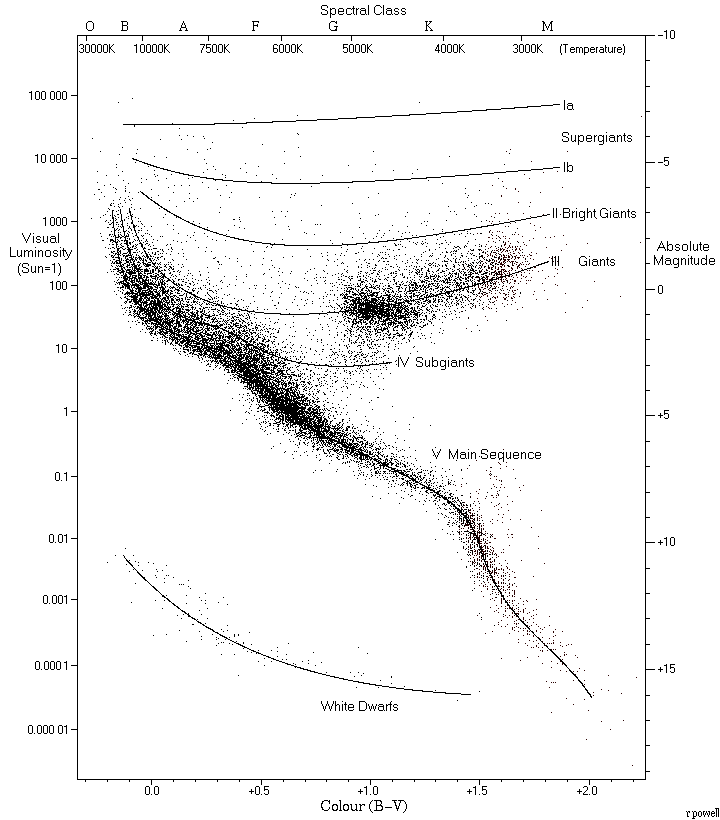
\includegraphics[width=0.5\textwidth]{hr}
  \caption{Diagramme de Hertzsprung-Russell des 22000 étoiles du
    catalogue Hipparcos et de 1000 étoiles faiblement lumineuses du
    catalogue Gliese des étoiles proches.}
  \label{hr}
\end{SCfigure}

\begin{Exercise}[Types spectraux]
  Donner approximativement le type spectral des étoiles dont le flux
  est maximal aux longueurs d'onde suivantes : 300~nm, 500~nm, et
  1,2~$\mu$m.  Peut-on déterminer la classe de luminosité ?

  Rappel de la loi de Wien : $\lambda_{\max} T = 2898$~\u{\micro m~K}.
\end{Exercise}

\begin{Answer}
  La loi de Wien permet de déterminer la température effective de
  chaque étoile, et ainsi d'en déduire une valeur approximative du
  type spectral. Ici seulement la première lettre est accessible, la
  détermination du chiffre suivant nécessiterait un tableau plus
  précis donnant les correspondances entre les sous-types et la
  température effective.
  \begin{center}
    \begin{tabular}{ccc}
      \toprule
      $\lambda_{\max}$ & $T_{\mathrm{eff}}(K)$ & Type spectral \\
      \midrule
      300 nm & 9660 & A  \\
      500 nm & 5796 & G \\
      1,2 $\mu$m & 2415 & M \\
      \bottomrule
    \end{tabular}
  \end{center}
  On ne peut pas déterminer la classe de luminosité grâce à la
  longueur d'onde du maximum du flux. Pour ceci, il faudrait connaître
  soit la luminosité de l'étoile, soit sa gravité de surface, soit son
  rayon.
\end{Answer}

\begin{Exercise}[Diagramme HR]
  Classer par ordre de température effective croissante, puis de rayon
  croissant, et enfin de luminosité croissante les étoiles de types
  spectraux suivants : M5III, O2V, K7I, A0VII.
\end{Exercise}

\begin{Answer}
  La séquence OBAFGKM décrit les types spectraux dans le sens des
  $T_{\mathrm{eff}}$ décroissantes, on aura donc dans le sens des
  $T_{\mathrm{eff}}$ croissantes : M5III, K7I, A0VII, et O2V.

  La classe de luminosité définit des groupes d'étoiles de rayon
  différent, on aura donc dans l'ordre croissant : A0VII, O2V, M5III,
  et K7I.

  Enfin, l'examen du diagramme HR montre qu'une étoile chaude de la
  séquence principale peut être plus lumineuse qu'une sous-géante
  froide, et on aura dans le sens des luminosités croissantes : A0VII,
  M5III, O2V, et K7I.

  Ceci montre que le terme «~classe de luminosité~» peut être source
  d'erreur.
\end{Answer}

\subsection{Mesure des rayons}

\begin{Exercise}[Interférométrie]
  Le tableau suivant donne le diamètre apparent $\theta_*$ des étoiles
  de l'exercice~\ref{exo:10}, mesuré par interférométrie. Calculer
  leur rayon $R$ (on rappelle les distances déterminées dans un
  exercice précédent) et, à l'aide de ce résultat, attribuer à chaque
  étoile sa classe de luminosité parmi les suivantes : I, III, V.
  \begin{center}
    \begin{tabular}{lccc}
      \toprule
      & $\alpha$ CMa & $\alpha$ Tau & $\alpha$ Ori \\
      \cmidrule(r){2-4}
      $\theta_*$ [mas] & 5,89 & 24 & 67 \\
      $d$ [pc] & 2,64  & 20  & 130 \\
      \bottomrule
    \end{tabular}
  \end{center}
\end{Exercise}

\begin{Answer}
  Pour Sirius, le rayon vaut $R[\u{UA}] = d[\u{pc}] \times
  \theta_*[''] / 2$ soit $R = \SI{7,8e-3}{ua} = \SI{1,67}{\Rsun}$.
  Le tableau suivant donne les résultats pour les 3 étoiles :
  \begin{center}
    \begin{tabular}{lccc}
      \toprule
      & $\alpha$ CMa & $\alpha$ Tau & $\alpha$ Ori \\
      \cmidrule(r){2-4}
      $R/\Rsun$ & 1,67 & 52 & 936 \\
      Classe de luminosité & V & III & I \\
      Type spectral & A1V & K5III & M2I \\
      \bottomrule
    \end{tabular}
  \end{center}
  Dans cet exemple, il est possible d'attribuer à chaque étoile sa
  classe de luminosité en utilisant le lien qui existe avec le rayon
  stellaire. Le type spectral complet est donné pour information.
\end{Answer}

\subsection{Mesure de masse (étoiles doubles)}

\begin{Exercise}[Système binaire]
  On observe une étoile double visuelle dont le plan de l'orbite est
  perpendiculaire à la ligne de visée.
  \begin{itemize}
  \item La parallaxe de ce système est de 100~mas.
  \item La plus grande séparation angulaire entre les deux composantes
    est de $5''$, et la plus petite de $1''$.
  \item La période de révolution est de 30~ans.
  % \item L'étoile primaire se trouve au foyer de l'orbite observée, car
  %   il n'y a pas d'effet de projection.
  \item Le compagnon est toujours observé à une distance du centre de
    gravité 5~fois plus grande que celle de l'étoile primaire.
  \end{itemize}
  Déterminer la masse de chaque composante.
\end{Exercise}

\begin{Answer}
  Les paramètres observés permettent de remonter aux données suivantes
  pour le système :
  \begin{itemize}
  \item La distance est $D[\u{pc}] = 1/p[''] = 10$~pc.
  \item La dimension angulaire du grand axe de l'orbite relative est
    de $5'' + 1'' = 6''$. Le demi-grand axe apparent est donc $\theta
    = 3'' = 1,45\e{-5}$~rad.
  \item Le demi-grand axe de l'orbite relative est donné par
    $a[\u{UA}] = \theta[''] D[\u{pc}]$ soit $a = 30\;\u{UA} =
    4,49\e{12}\;\u{m}$.
  \item La 3ème loi de Kepler (en unités réduites) donne la somme des
    masses : $M_{1} + M_{2} = 30\;\Msun = 5,97\e{31}$~kg.
  \item Les distances des étoiles $E_1$ et $E_2$ au centre de gravité
    $G$ vérifient $M_1 \times GE_1 = M_2 \times GE_2$. Le rapport des
    masses vaut donc $M_1 / M_2 = GE_2 / GE_1 = 5$.
  \item Finalement : $M_1 = 25\;\Msun$ et $M_2 = 5\;\Msun$
  \end{itemize}
\end{Answer}


\begin{Exercise}[Le paradoxe d'Algol]
  Le tableau suivant rappelle les caractéristiques du système binaire
  à éclipse d'Algol ($\beta$~Per):
  \begin{center}
    \begin{tabular}{lcc}
      \toprule
      $p$ (mas) & \multicolumn{2}{c}{35,14 $\pm$ 0,90} \\
      $T$ (jours) & \multicolumn{2}{c}{2,8674} \\
      $\theta_{\mathrm{rel}}$ [mas] & \multicolumn{2}{c}{2,283} \\
      \midrule
      Composantes & $A$ & $B$ \\
      \cmidrule(r){2-3}
      Type spectral & B8V & K2IV \\
      $R/\Rsun$ & 2,74 & 3,60 \\
      $\theta_{\mathrm{abs}}$ (mas) & & 1,872 \\
      \bottomrule
    \end{tabular}
  \end{center}
  On supposera l'orbite circulaire, ainsi le demi-grand axe de
  l'ellipse projetée est égal au rayon de l'orbite.

  \begin{enumerate}
  \item Quelle est la distance (et son erreur) de ce système ?
  \item Quelle est la séparation des deux étoiles ? Comparez-la à
    leurs rayons.
  \item Quelle est la masse de chacune des étoiles ? Compte-tenu des
    types spectraux, décrire le \emph{paradoxe d'Algol} et suggérer
    une solution.
  \end{enumerate}
\end{Exercise}

\begin{Answer}
  \begin{itemize}
  \item Distance : $D [\u{pc}] = 1/p[''] = 28,46 \pm 0,73$~pc.
  \item Le demi-grand axe de l'orbite relative est donné par $a
    [\u{UA}] = \theta [''] D [\u{pc}]$ soit $a = 0,065~\u{UA} =
    9,77\e{9}~\u{m} = 13,96\;\Rsun = 2,2 (R_{A}+R_{B})$.
  \item La 3ème loi de Kepler donne la somme des masses réduites
    ($\tilde{M} = M/\Msun$) : $\tilde{M}_A + \tilde{M}_B =
    \tilde{a}^3/\tilde{T}^2 = 4,46$ (avec $\tilde{a} = a[\u{UA}]$ et
    $\tilde{T} = T[\u{an}]$)
  \item Le rapport des demi-grands axes apparents de l'orbite relative
    $\theta$ et de l'orbite absolue de l'étoile secondaire $\theta_B$
    donne le rapport des masses : $\theta_B / \theta = a_B / a = M_A /
    (M_A + M_B) = 0,82$
  \item On obtient finalement les masses $M_A = 3,65\;\Msun$ et $M_B =
    0,80\;\Msun$.
  \end{itemize}
  Le tableau suivant récapitule les données physiques du système :
  \begin{center}
    \begin{tabular}{lcc}
      \toprule
      $D$ (pc) & \multicolumn{2}{c}{28,46 $\pm$ 0,73} \\
      $a/\Rsun$ & \multicolumn{2}{c}{13,96} \\
      \midrule
      & $A$ & $B$ \\
      \cmidrule(r){2-3}
      $M/\Msun$ & 3,65 & 0,80 \\
      \bottomrule
    \end{tabular}
  \end{center}
  On remarque que l'étoile la plus évoluée, $B$ ($B$ est une
  sous-géante rouge, tandis que $A$ est une étoile de la séquence
  principale) est pourtant la moins massive, ce qui est
  contre-intuitif en terme d'évolution stellaire (les étoiles les plus
  massives évoluent plus rapidement). On peut invoquer des transferts
  de masse au sein de ce système très serré pour expliquer ce
  paradoxe.
\end{Answer}

\section{Les systèmes planétaires}

\subsection{Les lois de Kepler}

\begin{Exercise}[Invariant de Runge-Lenz]
  On considère une particule $P$ de masse $m$, animée d'un mouvement
  non relativiste par rapport à un repère d'origine $O$. Ce mouvement
  est dû à un champ de forces $\vec{F} (\vec{r}) = - \grad U (r) $
  dérivant d'un potentiel central $U (r)$, où $\vec{r} = \vec{OP}$.

  À l'instant $t$ on note respectivement $\vec{v} (t)$, $\vec{a} (t)$
  et $\vec{p} (t)$ la vitesse, l'accélération et la quantité de
  mouvement de la particule $P$.

  \begin{enumerate}
  \item Montrer que la force $\vec{F}$ est radiale.
  \item Montrer que le vecteur moment cinétique $\vec{L} = \vec{r}
    \wedge \vec{p}$ est conservé au cours du mouvement.  En déduire
    que la trajectoire de $P$ est située dans un plan $\Pi$ que l'on
    caractérisera.
  \item Montrer que l'énergie mécanique $E= \dfrac{1}{2} m v^2 + U$
    est une constante du mouvement.
  \item Calculer $L$ à l'aide des coordonnées polaires $(r,\theta)$
    dans le plan $\Pi$ et en déduire la loi des aires.
  \end{enumerate}
  Dans toute la suite du problème, le potentiel est de la forme :
  $$
  U (r) = - \frac{k}{r} \qquad \text{avec} \qquad k>0
  $$
  On définit le \emph{vecteur de Runge-Lenz} :
  $$
  \vec{A} = \frac{1}{k} \, \vec{v} \wedge \vec{L} - \frac{\vec{r}}{r}
  $$
  \begin{enumerate}[resume]
  \item Montrer que le vecteur $\vec{A}$ est constant dans le temps,
    et qu'il appartient au plan $\Pi$.
  \item Montrer que :
    $$
    A^2 = 1+2 \, \frac{L^2 \, E}{mk^2}
    $$
    (On pourra utiliser les coordonnées polaires : en particulier $
    \vec{v} = v_r \, \vec{e}_r + v_{\theta} \, \vec{e}_{\theta} $).
    En déduire, lorsque $L$ est fixé, une borne inférieure pour
    l'énergie $E$.  Montrer que pour un mouvement circulaire, $E$ est
    égal à la borne inférieure.
  \item Calculer le produit scalaire $\vec{A}.\vec{r}$ en fonction de
    $L$, $m$, $k$ et $r$.  Établir alors l'équation polaire de la
    trajectoire sous la forme :
    $$
    r (\theta) = \frac{p}{1+e \, \cos \theta}
    $$
    \emph{Indication : on définira l'angle $\theta$ à partir de l'axe
      polaire dirigé selon le vecteur $\vec{A}$.}

    Vérifier que : $e =\|\vec{A}\|$ et exprimer $p$ en fonction de
    $L$, $m$ et $k$.
  \item Discuter la nature de la trajectoire suivant la valeur de $E$.
  \end{enumerate}
  Dans la suite du problème on se restreint au cas des \emph{états
    liés} : $E<0$. La trajectoire est alors une ellipse.
  \begin{enumerate}[resume]
  \item Déterminer son demi-grand axe $a$ et son demi-petit axe $b$ en
    fonction de $m$, $k$, $L$ et $E$.
  \item Quelle est la valeur maximale $L_0$ de $L$, l'énergie $E$
    étant fixée ?
  \item Quelle est la trajectoire pour $L=0$, et pour $L=L_0$ ?
  \item Calculer la période du mouvement en fonction de $m$, $k$ et
    $a$.
  \end{enumerate}
\end{Exercise}

\begin{Answer}
  \begin{enumerate}
  \item $\vec{F} = - (\partial U/\partial r) \vec{e}_{r}$.
  \item $\vec{L} = mr^{2}\dot{\theta}\vec{e}_{z}$ et $\d S/\d t = C/2$
    avec $C \equiv r^{2}\dot{\theta}$.
  \item $r = \dfrac{L^{2}/km}{1+A\cos\theta} = p/(1+e\cos\theta)$
  \item
    \begin{itemize}
    \item Si $E < 0$: système lié, $e < 1$, trajectoire elliptique;
    \item si $E = 0$: $e = 1$, trajectoire parabolique;
    \item si $E > 0$: système ouvert, $e > 1$, trajectoire
      hyperbolique.
    \end{itemize}
  \end{enumerate}
\end{Answer}

\begin{Exercise}[Orbite de Pluton]
  L'orbite de Pluton est très excentrique ($e=0,248$). Son demi-grand
  axe vaut 39,43~unités astronomiques (L'unité astronomique est
  définie comme le demi grand axe de l'orbite de la Terre). Montrer
  que Pluton peut être plus proche du Soleil que Neptune dont le
  demi-grand axe de l'orbite vaut 30,06~UA et l'excentricité~0,009.
\end{Exercise}

\begin{Answer}
  \begin{center}
    \begin{tabular}{lccc}
      \toprule
      & & Neptune & Pluton \\
      \cmidrule(r){2-4}
      Demi-grand axe [UA] & $a$ & 30,06 & 39,43 \\
      Excentricité & $e$ & 0,009 & 0,248 \\
      Périhélie [UA] & $d=a(1-e)$ & 29,79 & 29,65 \\
      Aphélie [UA] & $D=a(1+e)$ & 30,33 & 49,21 \\
      \bottomrule
    \end{tabular}
  \end{center}
  Du fait de la très grande excentricité de son orbite, Pluton, à son
  périhélie, est plus proche que Neptune du Soleil: $d_{P} < d_{N}$.
\end{Answer}

\begin{Exercise}[Vitesses périhélique et aphélique]
  Montrer que la vitesse angulaire d'un objet décrivant une orbite
  elliptique autour du Soleil augmente lorsqu'il s'en
  rapproche. Montrer que le rapport des vitesses au périhélie (point
  le plus proche du Soleil) et à l'aphélie (point le plus éloigné du
  Soleil) ne dépend que de l'excentricité de l'orbite.  Calculer ce
  rapport pour la Terre dont l'excentricité de l'orbite vaut 0,0167,
  puis pour la comète de Halley dont l'excentricité de l'orbite vaut
  0,97.
\end{Exercise}

\begin{Answer}
  \begin{enumerate}
  \item On a vu que $r^2\dot{\theta}$ est une constante. On a donc
    $\dot{\theta}=C/r^2$ et la vitesse angulaire augmente lorsque $r$
    diminue.

  \item L'expression de la vitesse est : $\vec{v} = \dot{r}\vec{i} +
    r\dot{\theta}\vec{j}$

    Le périhélie et l'aphélie correspondent à des extremum sur la
    trajectoire, c'est à dire que $\d r/\d\theta =0$ et donc,
    puisque $\dot{r} = \dot{\theta}~\d r/\d\theta$,
    $\dot{r}=0$. La vitesse s'écrit donc bien $v = r\dot{\theta}$

  \item Puisque $r^2\dot{\theta}=C$ et que $v = r\dot{\theta}$, on a
    $v = C/r$. En reprenant les résultats vus précédemment sur les
    ellipses, on trouve $r = a(1-e)$ au périhélie, et $r = a(1+e)$ à
    l'aphélie. Le rapport des vitesse $v_p$ au périhélie et $v_a$ à
    l'aphélie est donc :
    $$
    \frac{v_p}{v_a} = \frac{1+e}{1-e}
    $$
    Soit pour la Terre : $v_p/v_a = 1,034$, 
    et pour la comète de Halley : $v_p/v_a = 65,67$.
  \end{enumerate}
\end{Answer}

% \begin{Exercise}
%   En reprenant le raisonnement précédent, trouver l'équation de la
%   trajectoire d'une planète autour du Soleil si la force de
%   gravitation était en $1/r^3$ au lieu de $1/r^2$. En déduire que dans
%   ce cas, vous ne seriez pas en train de vous embêter à faire cet
%   exercice.
% \end{Exercise}

% \begin{Answer}
%   On reprend l'expression de l'équation différentielle en remplaçant
%   $y^2$ dans le membre de droite par $y^3$. On obtient l'équation
%   suivante :
%   $$
%   -C^2 y^2 \left( y + \frac{d^2y}{d \theta ^2} \right) = -G(\Msun
%   + M_p)y^3
%   $$
%   Qui se simplifie par :
%   $$
%   -C^2 y - C^2 \frac{d^2y}{d \theta ^2} = G(\Msun + M_p)y
%   $$
%   Qui devient, en réorganisant les différents termes :
%   $$
%   \frac{d^2y}{d \theta ^2} + \left[ 1 - \frac{ G(\Msun + M_p)
%     }{C^2} \right]y = 0
%   $$
%   Ou encore, en posant $\alpha = \left[ 1 - \frac{ G(\Msun + M_p)
%     }{C^2} \right]$
%   $$
%   \frac{d^2y}{d \theta ^2} + \alpha y = 0
%   $$
%   Il faut analyser les trois cas $\alpha < 0$, $\alpha > 0$ et $\alpha
%   = 0$.
%   \begin{description}
%   \item[$\alpha > 0$] On pose $\epsilon = \sqrt{\left|\alpha\right|}$
%     et l'équation différentielle s'écrit alors :
%     $$
%     \frac{d^2y}{d \theta ^2} + \epsilon^2 y = 0
%     $$
%     dont la solution s'écrit simplement :
%     $$
%     y = K\cos(\epsilon \theta + \phi)
%     $$
%     donc :
%     $$
%     r = \frac{C}{\cos(\epsilon \theta + \phi)}
%     $$
%     où $C$, $\phi$ et $\epsilon$ sont des constantes. Cette équation a
%     une singularité lorsque $\theta = (\pi/2 - \phi) /
%     \epsilon$. Lorsque $\theta$ approchera cette valeur, la planète
%     s'échappera puisqu'alors $r \to \infty$. La figure (\emph{pas
%       trouvé la figure}) montre la trajectoire correspondante pour les
%     valeurs des constantes suivantes : $\epsilon = 0,05$, $\phi=0$ et
%     $C=1$. La planète arrive à proximité de l'étoile par une des
%     branches infinies, et repart par l'autre après avoir décrit
%     quelques révolutions autour de l'étoile.

%   \item[$\alpha < 0$] Comme précédemment, on réécrit l'équation
%     différentielle :
%     $$
%     \frac{d^2y}{d \theta ^2} + \epsilon^2 y = 0
%     $$
%     Dont la solution est :
%     $$
%     y = A e^{\epsilon \theta} + B e^{- \epsilon \theta}
%     $$
%     donc :
%     $$
%     r = \frac{1}{A e^{\epsilon \theta} + B e^{- \epsilon \theta}}
%     $$
%     On voit cette fois que lorsque $\theta$ augmente $r$ diminue
%     exponentiellement. la planète s'effondrera donc sur l'étoile.

%   \item[$\alpha = 0$] L'équation différentielle a la forme suivante :
%     $$
%     \frac{d^2y}{d \theta ^2} = 0
%     $$
%     Dont la solution est :
%     $$
%     y = A \theta + B
%     $$
%     donc :
%     $$
%     r = \frac{1}{A \theta + B}
%     $$
%     Ici encore, la planète s'effondrera sur l'étoile. On voit donc que
%     si la loi de la gravitation était en $\frac{1}{r^3}$, il
%     n'existerait pas de trajectoire fermée dans le problème à deux
%     corps, et aucune planète ne pourrait graviter autour des étoiles.
%   \end{description}
% \end{Answer}


\begin{Exercise}[Satellite géostationaire]
  Sachant que la Lune décrit son orbite autour de la Terre en
  27,32~jours et que le demi grand-axe de son orbite vaut 384400~km,
  calculer l'altitude d'un satellite géostationaire. On supposera que
  la masse de la Lune est négligeable par rapport à celle de la Terre
  (la Terre est environ 80 fois plus massive que la Lune).
\end{Exercise}

\begin{Answer}
  La troisième loi de Kepler, telle que nous venons de la démontrer
  s'applique bien sûr aussi pour le système Terre-Lune et on a :
  $$
  \frac{a^3_L}{T^2_L} = \frac{G(M_T + M_L)}{4\pi^2}
  $$
  Où $a_L$ est le demi grand axe de l'orbite de la Lune, $T_L$ sa
  période orbitale et $M_L$ sa masse. Puisque la masse de la Lune peut
  être négligée par rapport à celle de la Terre, cette relation s'écrit :
  $$
  \frac{a^3_L}{T^2_L} = \frac{GM_T}{4\pi^2}
  $$
  De même, pour le satellite, l'hypothèse $M_S \ll M_T$ est encore plus
  justifiée, et on a :
  $$
  \frac{a^3_S}{T^2_S} = \frac{GM_T}{4\pi^2} = \frac{a^3_L}{T^2_L}
  $$
  La période d'un satellite géostationnaire est, par définition, de
  23h56 (car un satellite géostationnaire reste toujours au dessus du
  même point de la Terre dont la période de rotation est de 23h56). On
  a donc
  \begin{align*}
    T_S &= 23 \times 60 + 56 = 1435~\text{min} \\
    T_L &= 27,3 \times 24 \times 60 = 39312~\text{min}
  \end{align*}
  d'où l'on tire finalement $a_S = 42300$~km.  Cette valeur correspond
  à la distance entre le centre de la Terre et le satellite.
  L'altitude du satellite est donc : $a_S = 42300 - 6378 = 35922$~km
\end{Answer}

% ==============================================================================
\chapter{Vie des galaxies}


\section{Milieu interstellaire}

\subsection{Mise en évidence expérimentale}

\begin{Exercise}[Comptage d'étoiles]
  Dans une observation de comptage d'étoiles, toutes de même type, on
  constate que :
  \begin{itemize}
  \item pour une magnitude apparente $m\le7$, on compte un
    nombre d'étoiles $N(m)$ tel que $\log{N(m)} = 0,6\,m + 3$
  \item pour $m\ge9$, on obtient $\log{N(m)}=0,6\,m + 2,4$
  \end{itemize}

  \begin{enumerate}
  \item Déterminer l'extinction en magnitude $A$ due au nuage traversé
    quand on passe de $m=7$ à $m=9$.

  \item On sait que la magnitude absolue des étoiles de ce type est
    $M=5$.  Déterminer :
    \begin{itemize}
    \item La distance $r_{1}$ du front proche du nuage.
    \item L'épaisseur $r_{2}-r_{1}$ du nuage.
    \end{itemize}
  \end{enumerate}
\end{Exercise}

\begin{Answer}
  \begin{enumerate}
  \item On rappelle l'expression du module de distance $m-M =
    5\log(D/10\;\u{pc})$ soit $\log(D/1\;\u{pc}) = 0,2(m-M)+1$. Le
    nombre $N(m)$ d'étoiles de magnitude inférieure à $m$ correspond,
    en l'absence d'extinction, au nombre d'étoiles dans une sphère de
    rayon $D(m)$, càd $N(m) \propto D(m)^3$, soit $\log N(m) = 0,6 m +
    \beta$.  En présence d'extinction, on a $\log N(m) = 0,6(m-A) +
    \beta$.
  \item L'extinction est nulle jusqu'à la distance $r_1$ du front du
    nuage, donc :
    $$
    \log{N(m)} = 0,6 (7-0) + \beta = 0,6\times 7 + 3
    \quad\text{soit}\quad \beta=3.
    $$
    À la distance $r_2$ du bord éloigné du nuage, pour laquelle $m =
    9$, et l'extinction $A$ :
    $$
    \log{N(m)} = 0,6 (9-A) + \beta = 0,6\times 9 + 2,4
    \quad\text{d'où}\quad A = 1~\u{mag}.
    $$
  \item En écrivant l'équation du module de distance avec $M=5$ :
    \begin{itemize}
    \item à l'entrée du nuage, $m = 7 = 5\log{r_1/10\;\u{pc}}+M$ d'où
      $r_1 = 25,1$~pc
    \item à la sortie du nuage, $m = 9 = 5\log{r_2/10\;\u{pc}}+M+A$
      avec $A=1$ d'où $r_{2} = 39,8$~pc
    \end{itemize}
    On en déduit l'épaisseur du nuage : $r_2-r_1 = 39,8-25,1 = 14,7$~pc
  \end{enumerate}
\end{Answer}

\begin{Exercise}[Densité des galaxies dans l'Univers]
% D'après http://cc.oulu.fi/~jpoutane/teaching/ism07.html
  E.~Hubble (1934, \emph{The Distribution of Extra-Galactic Nebulae},
  ApJ, \textbf{79}, 8) a mesuré que le nombre de galaxies $N(m)$
  jusqu'à une certaine magnitude limite $m$ par degré carré décroît
  avec la latitude galactique\footnote{L'angle entre le plan
    galactique et l'objet considéré, compté positivement vers le pôle
    nord galactique.} $b$ (pour $|b| > 15\deg$).  Ainsi, la densité de
  galaxies semble diminuer à mesure que l'on s'éloigne des pôles de la
  Galaxie ($b = \pm 90\deg$). Cela ne reflète évidemment pas la
  distribution intrinsèque des galaxies dans l'Univers, mais résulte
  d'un effet d'absorption de la lumière par les particules de
  poussière contenues dans notre propre Galaxie.

  On suppose d'une part que la poussière est répartie de façon
  homogène dans le disque galactique ($b=0$) d'épaisseur $2h$, et
  d'autre part que toutes les galaxies sont des sources ponctuelles de
  même magnitude absolue $M$ et uniformément distribuées dans l'espace
  avec une densité $\rho$.

  \begin{enumerate}
  \item Exprimer l'épaisseur $\ell$ de poussière traversée à une
    latitude $b$.  En déduire l'extinction interstellaire $A(b)$, en
    notant $A_{0}$ l'atténuation en magnitude aux pôles galactiques.
  \item Dans ces conditions, montrer que le nombre cumulé $N(m,b)$ de
    galaxies par degré carré à la magnitude apparente $m$ et à la
    latitude $b$ est donné par :
    $$
    \log N (m,b) = 0,6\,m - 0,6\frac{A_{0}}{\sin b} + K.
    $$
    Exprimer la constante $K$ en fonction des données du problème.
  \item Hubble (1934) a mesuré, pour des galaxies de magnitude absolue
    moyenne $M=-14$ :
    $$
    \log N (m,b) = 0,6\,m - 0,15 \frac{1}{\sin b} - 4,50.
    $$
    En déduire la densité moyenne $\rho$ des galaxies dans l'Univers
    (en Mpc$^{-3}$).
  \end{enumerate}
\end{Exercise}

\begin{Answer}
  \begin{enumerate}
  \item $\ell = h/\sin b$ et $A = l \times A_{0}/h = A_{0}/\sin b$.
  \item $N(m,b) = \rho \times 4\pi d^{3}/3$ avec $\log(d/\u{pc})
    = 1+0,2(m-M-A)$ donc $\log N(m,b) = 0,6m - 0,6A - 0,6 M +
    \log(\rho/\u{pc}^{-3}) + \log(4\pi/3) + 3$.
  \item $\log(\rho/\u{pc}^{-3}) = -16,52$ soit $\rho =
    30~\u{Mpc}^{-3}$.
  \end{enumerate}
\end{Answer}

\subsection{Extinction sélective et rougissement}

\begin{Exercise}[Interprétation physique]
  Une étoile est située à 2~kpc de l'observateur sur une ligne de
  visée représentative des conditions moyennes du MIS, pour lesquelles
  l'extinction moyenne en bande $V$ est de 0,3~mag/kpc.  En admettant
  que cette extinction n'est due qu'à des grains dont les
  caractéristiques suivent :
  \begin{itemize}
  \item rayon $a = \SI{0,1}{\micro\meter}$,
  \item efficacité d'extinction $Q_{ext} = 1$,
  \item masse volumique : 1~g/cm$^{3}$,
  \item répartition des grains uniforme sur la ligne de visée ;
  \end{itemize}
  calculer :
  \begin{enumerate}
  \item la profondeur optique, puis la densité de colonne des grains
    le long de la ligne de visée,
  \item Le nombre de grain par unité de volume sur cette ligne de
    visée,
  \item la masse volumique des grains dans le MIS.
  \end{enumerate}
  En admettant que la densité moyenne d'atomes d'H est de l'ordre de
  8~atomes par cm$^3$, et en négligeant la présence des atomes
  d'autres éléments, calculer (on donne la masse du proton $m =
  1,67\e{-24}$~g) :
  \begin{enumerate}[resume]
  \item la masse volumique du gaz dans le MIS,
  \item le rapport (masse volumique des grains)/(masse volumique du
    gaz).
  \end{enumerate}
  Qu'en concluez vous sur le rôle des grains dans la matière du MIS ?
\end{Exercise}

\begin{Answer}
  \begin{align*}
    \text{Distance de l'étoile :} &\quad
    L = 2\;\u{kpc} = 6,17\e{21}\;\u{cm} \\
    \text{Section d'un grain :} &\quad
    s_g = \pi\,a^2 = \pi\,(10^{-5})^2 = \pi\,10^{-10}~\u{cm^{2}} \\
    \text{Extinction en V sur la ligne de visée :} &\quad
    A_V = 0,3~\u{mag/kpc}\times 2~\u{kpc} = 0,6~\u{mag} \\
    \text{d'où la profondeur optique :} &\quad
    \tau = \frac{0,6}{1,086} = 0,55 = n_g\,s_g\,L
  \end{align*}
  La densité de colonne est le nombre de grains dans un cylindre de
  longueur $L$ et de section unité. Si la densité de grains $n_g$ est
  constante, la densité de colonne est donc égale à $n_g L$
  $$
  n_g L = \frac{\tau}{s_g} = \frac{0,55}{\pi 10^{-10}} =
  1,75\e{9}~\u{grains/cm^2}
  $$
  On déduit de l'expression précédente la densité de grains $n_g$ :
  $$
  n_g = \frac{1,75\e{9}}{6,17\e{21}} = 2,82\e{-13}~\u{grain/cm^{3}}
  $$
  Masse volumique des grains dans le MIS :
  $$
  1\;\u{g/cm^{3}}\times \frac{4\pi a^{3}}{3}\;\u{cm^3/grain} \times
  2,82\e{-13}\;\u{grain/cm^3} = 1,18\e{-27}\;\u{g/cm^3}
  $$
  Masse volumique du gaz dans le MIS :
  $$
  8\;\u{atomes/cm^3} \times 1,67352\e{-24}\;\u{g/atome} = 
  1,34\e{-23}\;\u{g/cm^3}
  $$
  $$
  \frac{\text{Masse volumique des grains}}{\text{Masse volumique du gaz}} =
  \frac{1,18\e{-27}\;\u{g/cm^3}}{1,34\e{-23}\;\u{g/cm^3}} = 8,8\e{-5}
  $$
  Conclusion : les grains ne représentent qu'une fraction très faible de
  la masse de matière dans le MIS.
\end{Answer}

\begin{Exercise}[Rougissement et température]
  En admettant que l'on observe un objet à la température $T$, dont le
  spectre est donné par la loi de Planck :
  $$
  W(\lambda) = C\,\lambda^{-5}\,
  \left[\exp\left({\frac{hc}{\lambda\,kT}}\right)-1\right]^{-1}
  $$
  En présence d'une extinction $A(\lambda) = a/\lambda$, montrez que :
  \begin{enumerate}
  \item pour $\lambda \ll hc/kT$ (limite de Wien), dans la partie
    bleue du spectre, le spectre observé est celui d'un corps noir à
    une température $T'$, que l'on déterminera.
  \item pour $\lambda \gg hc/kT$ (limite de Rayleigh-Jeans), dans la
    partie rouge du spectre, le spectre observé est identique à celui
    de la source.
  \end{enumerate}
\end{Exercise}

\begin{Answer}
  $W(\lambda)$, donné par la formule de Planck, représente le flux de
  l'étoile en l'absence d'extinction.  Si $W'(\lambda)$ représente le
  flux de l'étoile en présence d'une extinction en magnitude de la
  forme $A(\lambda) = a/\lambda$, on a : $A(\lambda)= +2,5 \log W/W'$
  soit, en posant $a' = a \times 0,4 \ln 10$ : $W' = W
  \exp(-a'/\lambda)$.

  \begin{enumerate}
  \item Pour la partie du spectre aux courtes longueurs d'onde (régime
    de Wien), on a $hc/\lambda kT \gg 1$ d'où :
    \begin{align*}
      W  &\simeq C\lambda^{-5}\exp\left(-\frac{hc}{\lambda kT}\right)
      \quad\text{pour}\quad \lambda \ll hc/kT\\
      \text{donc}\quad
      W' &\simeq C\lambda^{-5}\exp\left(-\frac{hc}{\lambda kT}\right)
      \exp\left(-\frac{a'}{\lambda}\right) \\
      &\simeq C\lambda^{-5}\exp\left(-\frac{hc}{\lambda kT'}\right)
      \quad\text{avec}\quad
      \frac{1}{T'} = \frac{1}{T} + \frac{ka'}{hc}
    \end{align*}
    On retrouve pour $W'$ la forme de la formule de Plank (dans la
    limite de Wien), mais cette fois pour un corps à une température
    $T' < T$.

  \item Pour la partie du spectre aux grandes longueurs d'onde (régime
    de Rayleigh-Jeans), le terme $\exp(a'/\lambda)$ tend
    progressivement vers 1, donc $W'$ devient égal à $W$. Les spectres
    rougis et non rougis sont identiques.
  \end{enumerate}
\end{Answer}

\begin{Exercise}[Rougissement et couleur]
  Une étoile $G5V$ a une magnitude absolue $M_V= 5$, et un indice de
  couleur intrinsèque $(B-V)_0 =0,7$. On observe une étoile de ce type
  spectral, située à une distance de 5~kpc
  \begin{enumerate}
  \item Calculer les magnitudes apparentes $m_{V_0}$ et $m_{B_0}$
    qu'aurait cette étoile s'il n'y avait aucune extinction.
  \item L'étoile est située dans une région où l'extinction du MIS
    peut être caractérisée par :
    \begin{itemize}
    \item une extinction de 0,3~mag/kpc en bande $V$,
    \item une loi d'extinction de la forme : $A(\lambda) = A_V \times
      (\lambda_V/\lambda)$
    \end{itemize}
    Calculer les extinctions $A_V$ et $A_B$ qu'elle subit du fait de
    cette loi d'extinction
  \item Calculer l'excès de couleur $E_{B-V}$ de cette étoile par
    rapport à une étoile très proche de même type spectral.
  \item Calculer l'indice $(B-V)$ observé en présence d'extinction.
  \item À l'aide du diagramme HR, déterminer le type spectral apparent
    de l'étoile.
  \item Qu'en concluez vous sur l'effet de l'extinction sélective sur
    la «~couleur~» d'une étoile.
  \end{enumerate}

  On rappelle les longueurs d'onde effectives des bandes $V$ et $B$:
  $\lambda_{V}=550$~nm et $\lambda_{B}=440$~nm.
\end{Exercise}

\begin{Answer}
  \begin{enumerate}
  \item Magnitudes apparentes sans extinction
    \begin{align*}
      m_{V_0} &= M_{V} + 5\log(5\;\u{kpc}/10\;\u{pc}) = 18,5 \\
      m_{B_0} &= m_{V_0} + (B-V)_0 = 19,2
    \end{align*}
  \item Calcul des extinctions
    \begin{align*}
      A_V &= 5\;\u{kpc}\times 0,3\;\u{mag/kpc} = 1,5 \\
      A_B &= 1,5 \times 0,55/0,44 = 1,88
    \end{align*}
  \item Calcul de l'excès de couleur: $E_{B-V} = A_B - A_V = 1,88 -
    1,5 = 0,38$
  \item Calcul de l'indice de couleur: $(B-V) = (m_{B_0} + A_B) -
    (m_{V_0} + A_V) = (B-V)_0 + E_{B-V} = 0,7 + 0,38 = 1,08$
  \item Le type spectral apparent sera celui d'une étoile environ
    K5. Comme l'extinction ne change pas la profondeur des raies de
    l'étoile, sa classe de luminosité apparente restera celle d'une
    naine V. L'étoile apparaîtra donc comme une K5V.
  \item L'étoile paraît plus rouge que s'il n'y avait pas d'extinction.
  \end{enumerate}
\end{Answer}


\begin{Exercise}[Excès de couleur]
  On a déterminé par spectroscopie le type spectral $B2V$ pour une
  étoile lointaine. L'indice de couleur intrinsèque de ce type
  d'étoiles est $(B-V)_0 = -0,25$ . Par photométrie on a déterminé un
  indice de couleur observé $(B-V) = 2,25$.
  \begin{enumerate}
  \item Déterminer l'extinction $A_V$ de cette étoile à partir de la
    la loi de variation de $A_V/E_{B-V}$ en fonction de $1/\lambda$
    (Fig.~\ref{extinction}).
  \item Quelle sera l'extinction de cette étoile dans la bande
    photométrique infrarouge $K$ ?
  \item Qu'en concluez vous sur l'effet de l'extinction dans
    l'infrarouge, comparé à celui dans le visible ?
  \end{enumerate}
\end{Exercise}

\begin{SCfigure}[0.5]%[htp]
  \centering
  \includegraphics[width=0.5\textwidth]{interstellarreddeningreduite}
  \caption{Loi de couleur: $A_{\lambda}/E_{B-V}$ en fonction de
    $1/\lambda$. On y lit p.ex. que $A_{V}/E_{B-V} \simeq 3,1$.}
  \label{extinction}
\end{SCfigure}

\begin{Answer}
  \begin{enumerate}
  \item Calcul de l'extinction: $E_{B-V} = (A_B- A_V) = (B-V) -
    (B-V)_0 = 2,25 - -0,25 = 2,5$.  Le graphique donne $A_V/E_{B-V}
    \simeq 3,1$, d'où $A_V = 3,1 \times 2,5 = 7,75$.
  \item Le graphique donne $A_K/E_{B-V} \simeq 0,5$, d'où $A_K = 0,5
    \times 2,5 = 1,25$.
  \item L'extinction est beaucoup plus faible dans l'IR que dans le
    visible.
  \end{enumerate}
\end{Answer}

\section{Galaxies}

\subsection{Classification morphologique des galaxies}

\begin{Exercise}[Propriétés «~physiques~» de la classification]
  En vous servant du tableau~\ref{tab:hubble}, répondez aux questions
  suivantes :
  \begin{enumerate}
  \item Que peut-on dire sur la fraction de gaz dans les galaxies
    selon le type morphologique ?
  \item Que peut-on dire de la densité surfacique de masse, en
    supposant que toute la masse des galaxies est concentrée dans un
    disque mince ?
  \end{enumerate}
\end{Exercise}

\begin{table}  
  \centering
  \caption{Propriétés quantitatives de la séquence de Hubble.}
  \label{tab:hubble}
  \begin{tabular}{lcccccc}
    \toprule
    Propriétés & E,S0 & S0a,Sa & Sab,Sb & Sbc,Sc & Scd,Sd & Sm,Im \\
    \midrule
    $M_{\mathrm{totale}}$ ($10^{10}\Msun$) & & 22,6 & 32,4 & 19,0 & 7,9 & 1,6 \\
    $M_{\mathrm{gaz}}$ (H neutre en $10^{9}\Msun$) & 
    1,24 & 5,62 & 15,14 & 15,85 & 9,33 & 2,40 \\
    Diamètre (kpc) & 21,1 & 19,8 & 25,1 & 22,4 & 17,7 & 8,5  \\
    \bottomrule
  \end{tabular}
\end{table}

\begin{Answer}
  \begin{enumerate}
  \item La fraction de masse de gaz est donnée par le rapport de la
    masse de gaz à la masse totale. Ce rapport augmente des S0 aux
    irrégulières.
  \item La densité surfacique de masse est $S = M/ \pi R^2$. Elle
    diminue des S0 aux irrégulières.
  \end{enumerate}

  Dans le tableau ci-dessous, les valeurs de
  $M_{\mathrm{gaz}}/M_{\mathrm{totale}}$ et de $S$ sont obtenues
  statistiquement sur un échantillon de plusieurs milliers de
  galaxies. Ce ne sont donc pas les valeurs obtenues par le calcul
  direct sur les médianes, mais le comportement reste le même.
  \begin{center}
    \begin{tabular}{lcccccc}
      \toprule
      Propriétés & E,SO & S0a,Sa & Sab,Sb & Sbc,Sc & Scd,Sd & Sm,Im \\
      \midrule
      $M_{\mathrm{gaz}}/M_{\mathrm{totale}}$ & & 0,03 & 0,05 & 0,08 & 0,11 & 0,15 \\
      $S$ ($\Msun/\u{pc}^2$) &  & 188,9 & 154,7 & 124,2 & 91,4 & 74,5 \\
      \bottomrule
    \end{tabular}
  \end{center}
\end{Answer}


\subsection{Constituants des galaxies}

\begin{Exercise}[Les étoiles]
  Si l'on considère une sphère de rayon 10~kpc peuplée par $10^{11}$
  étoiles dont le rayon est égal à celui du Soleil, calculez la
  fraction de volume occupé par les étoiles.
\end{Exercise}

\begin{Answer}
  La fraction est de $10^{11} \times \left(\frac{0,7\e{6}}{10\times
      3,08\e{16}}\right)^{3}\approx 10^{-24}$.
\end{Answer}


\begin{Exercise}[La matière noire]
  On considère une galaxie et ses étoiles réparties uniformément en
  fonction de la distance au centre de la galaxie.  On désigne par
  $M(R)$ la masse totale des étoiles contenues \emph{à l'intérieur} de
  la sphère de rayon~$R$.
  \begin{enumerate}
  \item Si les étoiles sont animées d'un mouvement de rotation
    uniforme autour du centre de la galaxie, donner la relation entre
    l'accélération normale $a$ d'une étoile située à la distance $R$
    de ce centre et sa vitesse $V$.
  \item Écrire la relation fondamentale de la dynamique pour cette
    étoile. En déduire la relation entre $V$ et $R$. Comment varie
    alors $V$ en fonction de $R$ ?
  \item Dans les galaxies spirales, on observe au-delà d'un certain
    rayon $R_{0}$ que la vitesse de rotation du gaz et des étoiles
    atteint une valeur limite $V_{0} > 0$. Commentez.
  \item Quelle forme de la densité de masse $\rho(R)$ doit-on présumer
    pour atteindre une valeur constante de $V$ quand $R$ augmente ? On
    rappelle que, sous l'hypothèse de symétrie sphérique, $\d M =
    4\pi R^2 \rho(R)\,\d R$.
  \end{enumerate}
\end{Exercise}

\begin{Answer}
  \begin{enumerate}
  \item Accélération centripète : $a = V^2/R$
  \item PFD : $mV^2/R = GmM(R)/R^2$, soit $V^2 = GM(R)/R$ (orbite
    circulaire). Si $M(R)$ tend vers une valeur limite (la masse
    totale de la galaxie), $V$ doit alors décroitre avec $R$ avec la
    puissance $-1/2$ (décroissance képlérienne) donc tendre vers zéro.
  \item Si la vitesse tend vers une valeur plateau $V_0 > 0$, la
    repartition de masse dans la galaxie est à revoir : on introduit
    ainsi la notion de matière noire, qui n'est perceptible que par
    ses effets gravitationnels.
  \item $\d M(R)/\d R = 4\pi R^2 \rho(R) \stackrel{\mathrm{PFD}}{=}
    \d(RV_{0}^{2}/G)/\d R$ d'où $\rho(R) = (1/4\pi R^2) (V_0^2/G)
    \propto 1/R^{2}$. Problème: la masse totale de la galaxie diverge!
  \end{enumerate}
\end{Answer}

\subsection{Exemple de galaxie : la Voie Lactée }

% \begin{Exercise}[Morphologie de notre galaxie]
%   En examinant en détail l'image de notre galaxie prise par COBE/DIRBE
%   (Fig.~\ref{cobe}) on distingue que le bulbe de la Voie Lactée n'est
%   pas symétrique.  Donner une explication plausible de cette
%   asymétrie, en se rappelant notre position très particulière par
%   rapport au centre de notre galaxie, et en se rappelant des
%   différentes composantes qui composent notre Galaxie.
% \end{Exercise}

% \begin{figure}%[htp]
%   \centering
%   \includegraphics[width=0.8\textwidth]{milky2w}
%   \label{cobe}
%   \caption{Notre galaxie vue par COBE/DIRBE.}
% \end{figure}

% \begin{Answer}
%   Le bulbe de la galaxie vue en infrarouge est effectivement
%   asymétrique : le coté gauche a une épaisseur légèrement plus
%   grande que le coté droit. Ça n'est pas un effet de populations
%   stellaires, ou d'extinction due à la poussière, mais bien une
%   épaisseur réellement plus grande d'un coté que de l'autre. Ce que
%   l'on voit est en fait un effet de projection : c'est en fait la
%   barre de la Galaxie que nous observons. Cette barre étant inclinée
%   à 35° environ par rapport à nous, le coté gauche étant proche de
%   nous, le coté droit loin de nous (de l'autre coté du centre
%   galactique). Une des extrémités de la barre est donc plus proche
%   de nous, et par projection elle apparaît plus haute.
% \end{Answer}

\begin{Exercise}[Le centre galactique]
  La Fig.~\ref{centregalac} montre l'orbite de l'étoile ayant la plus
  grande vitesse autour du centre galactique. À partir des
  caractéristiques de cette orbite (période de $T = 15,2$~ans, et demi
  grand-axe de $a = 0\farcs 119$), retrouver l'estimation de la masse
  incluse dans ce rayon au centre de notre Galaxie en utilisant la
  troisième loi de Kepler. On rappelle que nous sommes à environ $R =
  8,5$~kpc du centre galactique.

  La masse \emph{visible} au centre galactique étant estimée à environ
  $10^{6}$ masses solaires, en déduire une estimation de la masse
  centrale invisible de notre Galaxie. Proposer une explication.
\end{Exercise}

\begin{SCfigure}[0.5]%[htp]
  \centering
  \includegraphics[width=0.5\textwidth]{nature01121-f2_2}
  \caption{Orbite de l'étoile S2 autour du centre galactique SgrA*
    (Schödel et al. 2002).}
  \label{centregalac}
\end{SCfigure}

\begin{Answer}
  En écrivant la 3\ieme loi de Kepler dans le système Terre-Soleil et
  dans le système S2-SgrA*, nous obtenons:
  $$
  \frac{(a/a_{\oplus})^{3}}{(T/T_{\oplus})^{2}} = M_{\mathrm{SgrA}*}/\Msun 
  \qquad\text{avec}\qquad 
  a~[\u{UA}] = a~[1''] \times R~[1~\u{pc}] = 1,011\e{3}
  $$
  d'où $M_{\mathrm{SgrA}*} = 4,5\e{6}\;\Msun \gg M_{\mathrm{visible}}$.
\end{Answer}

\subsection{Le groupe local}

\begin{Exercise}[Recensement]
  Dans la Table~\ref{listgalac}, compter le nombre de galaxies ayant
  un diamètre plus petit que 6~kpc, et celles ayant un diamètre plus
  grand. Quelles sont les galaxies qui dominent en nombre ? Et en
  luminosité totale ?
\end{Exercise}

\begin{table}%[htp]
  \caption{Galaxies du Groupe Local, avec leurs noms, leurs
    positions sur le ciel, le type de Hubble, la distance, les diamètres
    physiques et angulaires.}
  \label{listgalac}
  \centering
  \includegraphics[height=.95\textheight]{listegalaxiegroupelocal}
\end{table}

\begin{Answer}
  Il y a 26 petites galaxies -- dites «~naines~» -- sur les 30
  galaxies dont on nous donne la taille, et seulement 2 galaxies avec
  un diamètre de plus de 30~kpc : M~31 et la Voie Lactée. Ce sont donc
  les galaxies naines qui dominent en nombre, mais pas en luminosité
  totale.
\end{Answer}

\subsection{Distribution des galaxies dans l'univers}

% Schechter, 1976ApJ...203..297S
\begin{Exercise}[Fonction de luminosité]
  La fonction de luminosité $\Phi(L)$ des galaxies s'exprime
  généralement à l'aide de la fonction de Schechter (1976) :
  $$
  \Phi(L)\,\d L =
  \Phi^{*}\left(\frac{L}{L^{*}}\right)^{\alpha}
  \exp\left(-\frac{L}{L^{*}}\right)\,\d L/L^{*}
  $$
  où $\Phi(L)\d L$ est le nombre de galaxies de luminosité comprise
  entre $L$ et $L+\d{}L$ par unité de volume (p.ex. par
  Mpc$^{3}$). Pour les galaxies de champ, on a $\alpha \sim -5/4$,
  $L^{*}_{B} \sim 2\e{10}\;\Lsun$ et $\Phi^{*} \sim
  5\e{-3}$~Mpc$^{-3}$.
  \begin{enumerate}
  \item Quelle est la signification physique de la loi de Schechter ?
  \item Exprimer la loi de Schechter en magnitudes absolues.
  \end{enumerate}

  \begin{SCfigure}%[htp]
    \centering
    \includegraphics[width=0.4\textwidth]{schechter76}
    \caption{Fonction de luminosité des galaxies dans les amas d'Abell
      (Schechter, 1976).} 
    \label{schechter76}
  \end{SCfigure}
\end{Exercise}

\begin{Answer}
  \begin{enumerate}
  \item Cette fonction empirique montre bien la prédominance des
    galaxies de faible luminosité intrinsèque. Noter que le nombre
    total de galaxies $N_{T} = \int_{0}^{\infty} \Phi(L)\,\d L =
    \Phi^{*}\Gamma(\alpha+1)$ diverge pour $\alpha \leq -1$, mais que
    la luminosité totale $L_{T} = \int_{0}^{\infty} L\Phi(L)\,\d L =
    \Phi^{*}L^{*}\Gamma(\alpha+2)$ reste finie.
  \item On a $\Phi(L)\,\d L = \Phi(M)\,\d M$ avec $M - M^{*} = -2,5\log
    L/L^{*}$, d'où:
    $$
    \Phi(M) = 0,4 \ln 10\times \Phi^{*}\,10^{-0,4(\alpha
      +1)(M-M^{*})}\exp \left( -10^{-0,4(M-M^{*})} \right)
    $$
  \end{enumerate}

  \begin{SCfigure}[0.5]%[htp]
    \centering
    \includegraphics[width=0.6\textwidth]{schechter}
    \caption{Fonction (normalisée) de Schechter pour différentes
      valeurs de $\alpha$.}
    \label{schechter}
  \end{SCfigure}
\end{Answer}

%\subsubsection{Effets d'environnement, collisions et fusions}

\begin{Exercise}[Fréquence de collision dans un amas]
  On considère un amas de galaxies ayant les caractéristiques
  suivantes :
  \begin{itemize}
  \item il est supposé sphérique, de diamètre $D_{a}$,
  \item il contient $N_{g}$ galaxies identiques et réparties
    uniformément dans l'amas,
  \item les galaxies sont supposées animées d'une vitesse quadratique
    moyenne $v_{g}/\sqrt{2}$ (la vitesse \emph{relative} quadratique
    moyenne est donc $v_{g}$).
  \end{itemize}

  \begin{enumerate}
  \item Donner l'expression de la densité numérique de galaxies (le
    nombre par unité de volume) $n_{g}$ dans l'amas.

  \item On suppose que les galaxies ont un diamètre typique
    $d_{g}$. En modélisant les galaxies comme des sphères dures
    («~boules de billard~»), donner l'expression de la section
    efficace $S_{\mathrm{eff}}$ lors d'une interaction (collision)
    entre deux galaxies.

  \item Donner l'expression du nombre d'interactions que subit une
    galaxie de l'amas pendant un temps $\Delta t$. En déduire, pour
    une galaxie, le temps caractéristique de collision $\tau_{c}$ et
    le libre parcours moyen $\ell_{c}$.

  \item En déduire le temps $T_{c}$ entre deux interactions au sein de
    l'amas.

  \item Application numérique : considérons un amas avec $D_{a} =
    7$~Mpc, $N=850$ galaxies, $d_{g} = 20$~kpc et $v_{g} =
    650$~km/s. Explicitez le calcul numérique du temps moyen entre
    deux collisions pour cet amas.
  \end{enumerate}
\end{Exercise}

\begin{Answer}
  \begin{enumerate}
  \item Le volume de l'amas est $V_{a} = \pi D_{a}^3/6$ et la densité
    numérique de galaxies est donc $ n_{g} = N_{g}/V_{a} = 6N_{g}/\pi
    D_{a}^3$.

  \item Deux galaxies entreront en collision lorsqu'elle passent à une
    distance $< d_{g}$ l'une de l'autre. La section efficace de
    collision est donc l'aire du disque de rayon $d_{g}$ :
    $S_{\mathrm{eff}} = \pi d_{g}^{2}$.

  \item Considérons une galaxie. Le volume utile «~balayé~» par cette
    galaxie pendant le temps $\Delta t$ est $\Delta V = v_{g} \times
    S_{\mathrm{eff}} \times \Delta t$. Le nombre de collisions que
    subira cette galaxie pendant le temps $\Delta t$ est donc égal au
    nombre de galaxies dans le volume $\Delta V$ : $N_{c} = n_{g}
    \Delta V$. Le temps caractéristique de collision $\tau_{c}$
    correspond au $\Delta t$ tel que $N_{c} = 1$ ; le libre parcours
    moyen est $\ell_{c} = v_{g} \times \tau_{c}$:
    $$
    \tau_{c} = \frac{D_{a}^3}{6 N_{g} d_{g}^2 v_{g}}, 
    \qquad
    \ell_{c} = \frac{D_{a}^3}{6 N_{g} d_{g}^2}
    $$

  \item Application numérique : $v_{g} = 650\;\u{km/s} =
    665\;\u{kpc/Gan}$, $\tau_{c} = 253$~Gan, $T_{c} = \tau_{c}/N_{g} =
    297$~Man.
  \end{enumerate}
\end{Answer}


\subsection{Équilibre gravitationnel}

\begin{Exercise}[Théorème du Viriel scalaire]
  On considère le système Terre-Soleil. Le Soleil, de masse $\Msun$,
  est pris comme référence du mouvement ($v_\odot = 0$). On note
  $M_\oplus$ et $v_\oplus$ la masse et la vitesse de la Terre.
  \begin{enumerate}
  \item Écrire l'expression de l'energie cinétique du système
    Terre-Soleil.
  \item Énoncer le théorème du Viriel. En déduire l'expression de la
    distance $D$ d'équilibre entre la Terre et le Soleil. Faire
    l'application numérique, sachant que $\Msun = 2\e{30}$~kg,
    $M_\oplus = 5,97\e{24}$~kg et $v_\oplus = 30$~km/s.
  \item On considère un système d'étoiles binaires en équilibre. Pour
    simplifier, les étoiles sont prises de masses égales $M_{1} =
    M_{2} = \Msun$ et leurs vitesses sont considérées comme égales
    $v_1 = v_2 = v$.

    Expliciter la relation entre la distance entre ces deux étoiles et
    leur vitesse et calculer cette vitesse $v$ pour les distances
    d'équilibre $D$ suivantes : 1~UA, 10~UA et 100~UA.
  \end{enumerate}
\end{Exercise}

\begin{Answer}
  \begin{enumerate}
  \item $K = 1/2 M_\oplus v_\oplus^2$
  \item Théorème du Viriel : $2K + U = 0$ avec $U = -G\Msun
    M_\oplus/D$ d'où $D = G\Msun/v_\oplus^2 = 1$~UA.
  \item $K = 1/2\,M_{1}v_{1}^{2} + 1/2\,M_{2}v_{2}^{2} =
    \Msun v^{2} \stackrel{\mathrm{Viriel}}{=} -U/2 =
    +G\Msun^{2}/(2D)$ d'où $v = \sqrt{G \Msun/(2 D)}$, soit:
    \begin{center}
      \begin{tabular}{lccc}
        \toprule
        $D$ [UA]   & 1    & 10  & 100 \\
        \midrule
        $v$ [km/s] & 21,1 & 6,7 & 2,1 \\
        \bottomrule
      \end{tabular}
    \end{center}
  \end{enumerate}
\end{Answer}

\begin{Exercise}[Autres applications du théorème du Viriel]
  On va maintenant utiliser le théorème du Viriel pour remplir le
  tableau ci-dessous, donnant les rayons, masses et vitesse
  caractéristiques de différents système stellaires.  
  \begin{center}
    \begin{tabular}{lrrr}
      \toprule
      Système & $R$ & $V$ [km/s] & $M/\Msun$ \\ 
      \midrule
      Amas globulaire  & 10~pc  & 10   & \corrige{$4,6\e{5}$} \\ 
      Galaxie          & 15~kpc & 200  & \corrige{$2,8\e{11}$} \\ 
      Amas de galaxies & 1~Mpc  & 1000 & \corrige{$4,6\e{14}$} \\ 
      \bottomrule
    \end{tabular}
  \end{center}
\end{Exercise}

\begin{Answer}
  On a $U = -GM^{2}/(2R)$ et $K=1/2\, MV^{2}$ d'où $M = 2RV^{2}/G$,
  avec $G = 6,67\e{-11}\;\u{m^{3}~kg^{-1}~s^{-2}} =
  4,302\e{-3}\;\u{km^{2}~s^{-2}~pc~\Msun^{-1}}$.
\end{Answer}

\begin{Exercise}[Temps cinématique]
  On va maintenant calculer le temps cinématique $t_c$ pour différents
  systèmes stellaires. 
  \begin{center}
    \begin{tabular}{lrrr}
      \toprule
      Système & $R$ & $M/\Msun$ & $t_c$ [ans] \\ 
      \midrule
      Amas ouvert      & 1~pc   & 500      & \corrige{$9,4\e{5}$} \\ 
      Amas globulaire  & 10~pc  & $10^5$   & \corrige{$2,1\e{6}$} \\ 
      Galaxie          & 15~kpc & $10^{11}$ & \corrige{$1,2\e{8}$} \\ 
      Amas de galaxies & 1~Mpc  & $10^{14}$ & \corrige{$2,1\e{9}$} \\
      \bottomrule
    \end{tabular}
  \end{center}
  Que remarquez-vous sur ces temps cinématiques pour les différents
  systèmes ?
\end{Exercise}

\begin{Answer}
  $t_{c} = R/V = \sqrt{2R^{3} / GM}$ avec $G =
  4,500\e{-15}$~\u{pc^{3}~\Msun^{-1}~an^{-2}}.

  Les temps cinématiques pour un amas ouvert et un amas globulaire ne
  sont pas vraiment différents malgré leurs tailles respectives très
  différentes.  De même entre une galaxie et un amas globulaire : il
  ne faut qu'environ 100$\times$ plus de temps à une étoile avec une
  vitesse typique pour traverser une grosse galaxies qu'un amas
  globulaire (bien sur les vitesses caractéristiques ne sont pas les
  mêmes pour ces deux systèmes).
\end{Answer}

% ==============================================================================

\chapter{Cosmologie}

\section{Espace et temps absolus}

\begin{Exercise}[La faiblesse de la force de gravitation]
  Marcel et Naomi ressentent l'un pour l'autre une certaine
  attirance...  Quelle part en revient tout bêtement à la force de
  gravitation universelle, lorsque leurs centres de gravité respectifs
  sont distants de 1 mètre ?  Quelle masse $m$, au même point de la
  Terre, présente un poids égal à cette force ?  Marcel pèse 700~N, et
  Naomi 580~N.  Le rayon de la Terre sera supposé égal à $R_{\oplus} =
  6370$~km, et la masse de la Terre est de $M_{\oplus} =
  5,97\e{24}$~kg.
\end{Exercise}

\begin{Answer}
  Il s'agit d'appliquer la formule de Newton deux fois pour trouver
  les masses respectives de Marcel et Naomi, puis une troisième fois
  pour calculer l'attraction qui s'exerce entre eux: $F_{MN} = G\,m_M
  m_N/d^2 = G\,m M_{\oplus}/R_{\oplus}^2$.  Pour Marcel,
  $P_{\mathrm{M}} = G M_{\mathrm{M}}M_{\oplus} / R_{\oplus}^2$ soit
  $M_{\mathrm{M}} = P_{\mathrm{M}}R_{\oplus}^2 / (G M_{\oplus}) =
  71,3~\u{kg}$. Pour Naomi, on peut utiliser le fait que
  $M_{\mathrm{N}}/M_{\mathrm{M}} = P_{\mathrm{N}} / P_{\mathrm{M}}$,
  puisque les deux personnes sont soumises au même champ de gravité,
  donc $M_{\mathrm{N}} = M_{\mathrm{M}}\times
  P_{\mathrm{N}}/P_{\mathrm{M}} = 71,3 \times 580/700 = 59,0~\u{kg}$
  d'où $F_{\mathrm{NM}} = 2,81\e{-7}~\u{N}.$ La masse qui présente un
  poids égal à cette valeur est de $m =
  F_{MN}R_{\oplus}^{2}/(GM_{\oplus}) = 2,86\e{-8}\;\u{kg} =
  \SI{28,6}{\micro g}$.

  L'attraction gravitationnelle est une force \emph{très faible},
  c'est même la plus faible des quatre forces fondamentales de
  l'Univers.
\end{Answer}

% \subsection{Problèmes de l'Univers de Newton}

% \begin{Exercise}[L'instabilité gravitationnelle]
%   Pourquoi Newton pense-t-il que ces trois hypothèses supplémentaires
%   permettraient, chacune, de «~sauver~» l'Univers de la catastrophe
%   gravitationnelle ?
% \end{Exercise}

% \begin{Answer}
%   \begin{itemize}
%   \item Si l'Univers est infini, tout point est entouré d'une
%     distribution de matière à symétrie sphérique, et restera donc
%     immobile.
%   \item Si l'Univers est en expansion, c'est qu'il n'est pas en train
%     de se contracter !
%   \item Si l'Univers est très jeune, il n'a pas encore eu le temps de
%     démarrer sa contraction gravitationnelle de façon sensible.
%   \end{itemize}
% \end{Answer}

% \begin{Exercise}[Le paradoxe d'Olbers]
%   En quoi le fait que l'Univers soit jeune et en expansion peut-il
%   permettre d'expliquer la noirceur du ciel nocturne ?
% \end{Exercise}

% \begin{Answer}
%   \begin{itemize}
%   \item Si l'Univers est jeune, du fait de la vitesse finie de
%     propagation de la lumière, celle qui provient des objets très
%     lointains n'a pas eu le temps de nous parvenir.
%   \item Si l'Univers est en expansion, la lumière qui nous parvient
%     des objets très lointains a été affaiblie par cette expansion
%     (ceci sera traité plus loin dans le cours), au point de ne pas
%     être détectable.
%   \end{itemize}
% \end{Answer}

\section{La rupture relativiste}

% \subsection{Vitesse de la lumière}

% \begin{Exercise}[La première mesure de $c$]
%   Si Roemer a fait le calcul (ce que l'on ignore, mais cela semble
%   assez probable), et en supposant qu'il utilisait la même valeur de
%   la distance Terre-Soleil que les astronomes d'aujourd'hui, quelle
%   valeur de $c$ a-t-il obtenue ?
% \end{Exercise}

% \begin{Answer}
%   Si la lumière met $8+8 = 16$~min pour traverser l'orbite de la
%   Terre, c'est à dire pour franchir une distance de 2~U.A., sa
%   vitesse est $c = 2 \times 1,49598\e{11} / ( 16 \times 60 ) =
%   3,11\e{8}$~m/s. Ceci suppose que la valeur de l'U.A. admise alors
%   était la même qu'aujourd'hui, ce qui n'est certainement pas exact
%   : en 1675, on n'avait pas encore très bien mesuré la distance de
%   la Terre au Soleil... La valeur de deux fois huit minutes est
%   elle-même approximative. Roemer aurait plutôt trouvé $2\e{8}$~m/s,
%   dit-on. La première détermination sérieuse de l'Unité Astronomique
%   est due à Cassini et Richer, en 1671. Il faudra attendre le XXe
%   siècle et les méthodes d'écho radar pour disposer de mesures très
%   précises de cette valeur.
% \end{Answer}

\subsection{Relativité générale}

\begin{Exercise}[L'équivalence gravité/accélération]
  Pour la Relativité Générale, gravitation et accélération sont
  équivalentes, mais cette équivalence n'est que \emph{locale}: aucune
  expérience de physique ne permet de distinguer les effets de l'une
  de ceux de l'autre, \emph{à condition} de se limiter à un «~petit~»
  domaine spatial.

  En reprenant l'expérience de pensée de l'«~ascenseur d'Einstein,~»
  pouvez-vous montrer qu'il est en effet facile de distinguer
  pesanteur et accélération par la fusée si on abandonne la localité.
\end{Exercise}

\begin{Answer}
  À grande échelle, le champ de gravité qui environne un corps massif
  reste en général discernable d'une accélération constante.  Par
  exemple, dans l'image de l'ascenseur d'Einstein, il ne faut pas que
  la cabine soit trop étendue.  Sinon, le parallélisme ou le
  non-parallélisme des forces sur des masses éloignées l'une de
  l'autre trahirait la «~vraie~» nature du champ.  Sur la
  Fig.~\ref{grav}, la cabine de gauche, supposée accélérée vers le
  haut (flèche bleue), produit des forces parallèles (flèches rouges)
  sur les deux masses-test.  La cabine de droite, immobile dans le
  champ de gravitation de la Terre, montre des forces convergentes
  vers le centre de la Terre (flèches vertes).  De même, le physicien
  pourrait mettre en évidence une dépendance de la force avec
  l'altitude dans le cas de droite.
  \begin{SCfigure}%[htp]
    \centering
    \includegraphics[width=0.4\textwidth]{grav}
    \caption{}
    \label{grav}
  \end{SCfigure}
\end{Answer}

\subsection{Les tests}

\begin{Exercise}[Le décalage gravitationnel vers le rouge]
  Une lampe spectrale émettant dans la raie H$\alpha$ ($\lambda_{0} =
  656,3$~nm) est utilisée pour communiquer à partir d'une capsule en
  orbite serrée autour d'une étoile à neutrons. Le rayon de l'orbite
  est $R=1000$~km, la masse de l'étoile de $M=1,5$~\u{\Msun}.  À
  quelle longueur d'onde $\lambda$ le vaisseau qui a lancé la capsule,
  et se tient prudemment à grande distance, doit-il rechercher les
  signaux ?

  Comparer cet effet gravitationnel au décalage par effet Doppler du
  signal de la sonde en orbite circulaire autour de l'étoile à
  neutrons.
\end{Exercise}

\begin{Answer}
  Le décalage gravitationnel subi à la distance $R$ d'un corps de
  masse $M$ s'écrit :
  \begin{align*}
    z_{G} &= \frac{GM}{c^2 R} = \frac{ 6,672\e{-11} \times 1,5 \times
      1,989\e{30} }{ 299792458^{2}\e{6} } = 2,216\e{-3} \\
    &= \frac{\lambda - \lambda_{0}}{\lambda_0}
  \end{align*}
  d'où $\lambda = (1+z_{G})\lambda_0 = 1,00221 \times 656,3 = 657,75$~nm.

  La vitesse de l'orbite circulaire de rayon $R$ autour d'une masse
  $M$ est donnée (dans l'approximation non-relativiste) par:
  $$
  v = \sqrt{\frac{GM}{R}} = 14112\;\u{km/s} \simeq 4,71\e{-2} \times c
  $$
  Le décalage par effet Doppler (dans la même approximation non
  relativiste) est donc $z_{D} = v/c = \sqrt{z_{G}} \gg z_{G}$.
\end{Answer}


\section{Le Big Bang}

\subsection{Film des débuts}

\begin{Exercise}[Nucléosynthèse primordiale ou non ?]
  Les éléments légers $\mathrm{H}$, ${}^{2}\mathrm{H}$,
  ${}^{3}\mathrm{H}$, ${}^{4}\mathrm{He}$, ${}^{7}\mathrm{Li}$ sont
  nés avec le Big Bang. Mais d'où proviennent tous les autres éléments
  «~lourds~», ceux qui entrent dans la composition des objets du
  quotidien ?
\end{Exercise}

\begin{Answer}
  Les chapitres traitant des modèles stellaires et de l'évolution
  stellaire nous fournissent la réponse :
  \begin{itemize}
  \item Jusqu'au ${}^{56}\mathrm{Fe}$, les noyaux sont produits par
    les étoiles.  La source d'énergie de celles-ci est d'origine
    thermonucléaire, et elles sont des usines à fabriquer, par fusion,
    des noyaux lourds à partir de noyaux plus légers.
  \item Au-delà, seules les explosions de supernovae atteignent des
    températures suffisantes (plusieurs $10^9$~K) pour pouvoir
    synthétiser les noyaux très lourds, jusqu'aux éléments
    transuraniens.
  \item Quelques noyaux particuliers (${}^{6}\mathrm{Li}$,
    ${}^{9}\mathrm{Be}$, ${}^{10}\mathrm{B}$) sont sans doute formés
    lors des collisions des rayons cosmiques avec la matière
    interstellaire.
  \end{itemize}
\end{Answer}

\subsection{Expansion de l'Univers...}

\begin{Exercise}[... limitée par \emph{c} ?]
  Plus une galaxie est éloignée de notre Voie Lactée, plus les
  astronomes lui trouvent une vitesse d'éloignement élevée. C'est
  l'expansion de l'Univers. Mais, quand la distance croît sans cesse,
  elle atteint un moment une valeur $d_c$ telle que :
  $$
  V = H_0 d_c > c
  $$
  Étonnant, non ?
\end{Exercise}

\begin{Answer}
  Il est interdit par la Relativité Générale de mesurer une vitesse
  égale ou supérieure à $c$ pour un objet de masse non nulle, comme
  une galaxie. Cependant, cette limite ne s'applique pas à l'expansion
  de l'Univers, où les objets (p.ex. les galaxies) sont immobiles dans
  un espace dont la géométrie s'étire. Les galaxies très lointaines
  voient effectivement leur vitesse apparente atteindre celle de la
  lumière, et disparaissent alors de l'Univers observable. Ceci
  n'enlève rien au fait qu'elles continuent à s'éloigner de nous à des
  vitesses supérieures à $c$.  Signalons que nos moyens d'observation
  actuels sont loin de nous permettre d'observer les objets qui
  s'approchent de cette limite.
\end{Answer}

\begin{Exercise}[... la même partout ?]
  La radiogalaxie 3C~171 (la 171e entrée dans le troisième catalogue
  de radiources établi par l'observatoire de Cambridge) est
  relativement lointaine; entraînée par l'expansion de l'Univers, elle
  présente une vitesse de fuite de 63\,000~km/s.

  Montrer que malgré cela, l'astronome Pr.~Snurp, qui a là-bas
  découvert l'expansion de l'Univers, comme Hubble l'a fait pour nous,
  a lui aussi trouvé une loi qui s'écrit :
  $$
  v_0 = X_0 d_{0},
  $$
  $v_0$ étant la vitesse mesurée à partir de 3C~171 pour une galaxie
  lointaine située à la distance $d_0$ de 3C~171, et que la constante
  de Snurp $X_0$ partage la valeur de $H_{0}$.

  Ainsi, d'une planète de 3C~171, comme de la Terre, on observe la même
  expansion universelle, avec la même géométrie, et le même taux...
\end{Exercise}

\begin{Answer}
  Désignons par $v_T$ et $d_T$ les vitesses et distances mesurées à
  partir de la Terre, $v_{3C}$ et $d_{3C}$ celles mesurées à partir de
  3C~171.  La vitesse de récession de 3C~171 mesurée de la Terre est
  donc $v_T(3C\;171) = 63\;000$~km/s.

  Considérons une autre galaxie, $G$, observée à la fois de la Terre
  et de 3C~171. On peut écrire :
  \begin{align*}
    \vec{v}_{3C}(G) &= \vec{v}_{3C}(T) + \vec{v}_{T}(G) \\
    &= -\vec{v}_{T}(3C\;171) + \vec{v}_{T}(G) \\
    &= -H_0\vec{d}_{T}(3C\;171) + H_0\vec{d}_{T}(G) \\
    &= H_0 \left[ \vec{d}_{T}(G) - \vec{d}_{T}(3C\;171) \right ] \\
    &= H_0 \vec{d}_{3C}(G)
  \end{align*}
  et donc, à partir de 3C~171 comme de la Terre, toute les galaxie
  observée semble s'enfuir avec une vitesse proportionnelle à sa
  distance, et le facteur de proportionnalité (la constante de Snurp)
  est universel : $X_0=H_0$ (Fig.~\ref{H0}).

  \begin{SCfigure}%[htp]
    \centering
    \includegraphics[width=0.4\textwidth]{351922_281}
    \caption{}
    \label{H0}
  \end{SCfigure}
\end{Answer}

\subsection{Constante de Hubble \& Co.}

Dans les exercices suivants, on supposera la constante de Hubble égale
à $H_0 = 70$~\u{km~s^{-1}~Mpc^{-1}}.

\begin{Exercise}[Le facteur d'expansion de l'espace]
  La constant de Hubble $H_0$ est usuellement exprimée en kilomètres
  par seconde et par mégaparsec, mais cela ne parle guère au sens
  commun.  Quelle est la valeur de l'accroissement annuel d'un
  kilomètre ?
\end{Exercise}

\begin{Answer}
  $1\;\u{Mpc} = 3,09\e{19}\;\u{km}$ et $1\;\u{an} = 3,16\e7\;\u{s}$,
  donc $71\;\u{km~s^{-1}~Mpc^{-1}} = 2,27\e{-18}\;\u{km~s^{-1}~km^{-1}}
  = 71,6\;\u{nm~an^{-1}~km^{-1}}$.
\end{Answer}

\begin{Exercise}[Temps de Hubble]
  Calculez le temps de Hubble $t_{H} = 1/H_{0}$. Quelle est sa
  signification physique ?  Quelle conclusion pouvez-vous en tirer sur
  l'âge de l'Univers ?
\end{Exercise}

\begin{Answer}
  Le temps de Hubble est défini par $1/t_{H} = H_0 =
  70\;\u{km~s^{-1}~Mpc^{-1}} = 2,27\e{-18}\;\u{s^{-1}}$ d'où $t_{H} =
  4,41\e{17}~s \simeq 13,97\e{9}$~ans. Il représente l'âge de
  l'Univers dans le cas d'un taux d'expansion \emph{constant}. On peut
  donc penser que l'Univers est âgé d'environ 14~Gans.
\end{Answer}

\begin{Exercise}[Densité critique]
  Calculer la densité critique $\rho_{C} = \dfrac{3 H_{0}^{2}}{8\pi G}$.
  Quelle est sa dimension ?  La convertir en nucléons/$\u{m^{3}}$ ($m_{p}
  \simeq m_{n} \simeq m_{u} = 1,66\e{-27}$~kg), puis en $\Msun/\u{Mpc}^{3}$.
  Commenter.
\end{Exercise}

\begin{Answer}
  $\rho_{C} = 9,20\e{-27}~\u{kg\;m^{-3}} = 5,54\;\text{nucléons}\;\u{m^{-3}} =
  1,34\e{11}\;\Msun\;\u{M\pc}^{-3}$, soit environ une galaxie (massive) par
  \u{M\pc^{3}}, densité caractéristique de l'Univers local.
\end{Answer}

\begin{Exercise}[Âge de l'Univers]
  À partir de la définition de $H_0$ et de la relation $R \propto
  t^{2/3}$ entre le facteur d'échelle $R$ et le temps $t$ dans le cas
  d'un Univers euclidien ($k=0$) dominé par la matière
  ($\Omega_{M}=1$, $\Omega_{\Lambda}=0$), trouver la relation entre
  $H_{0}$ et $t$.
\end{Exercise}

\begin{Answer}
  \begin{align*}
    H_0 &\defeq \frac{1}{R}\frac{\d R}{\d t} \\
    &= \left ( \frac{t}{t_0} \right )^{-2/3} \times
    \frac{\d\left( t/t_0 \right )^{2/3}}{\d t} 
    = \left ( \frac{t}{t_0} \right )^{-2/3} \times
    \left( \frac{t}{t_0} \right)^{-1/3} \frac{2}{3} \frac{1}{t_0} 
    = \left( \frac{t}{t_0} \right)^{-1} \times \frac{2}{3t_0} \\
    &= \frac{2}{3t} \\
    \text{donc}\quad t &= \frac{2}{3\,H_{0}}
  \end{align*}
  Pour un Univers critique dominé par la matière, l'âge de l'Univers
  est égal aux deux-tiers du temps de Hubble.
\end{Answer}

\section{Modèles cosmologiques}

\begin{Exercise}[Modèle FLRW]
  Dans le cas d'un Univers de Friedmann-Lemaître-Robertson-Walker à
  courbure spatiale nulle ($k=0$), on a :
  \begin{equation}
    \left(\frac{\dot{R}}{R}\right)^{2} = 
    \frac{\Lambda}{3} + \frac{8\pi G}{3}\rho.
    \label{eq:1}
  \end{equation}
  Par ailleurs, l'équation de conservation de l'énergie s'écrit
  toujours:
  \begin{equation}
    \label{eq:2}
    \dot{\rho} = -3\left(\rho + \frac{P}{c^{2}}\right)\frac{\dot{R}}{R}.
  \end{equation}

  \begin{enumerate}
  \item Que signifient les différents termes -- $R$, $\Lambda$, $\rho$
    -- de l'équation~(\ref{eq:1}) ? Quelle est la dimension de
    $\dot{R}/R$ ?  Comment s'appelle cette quantité ?

  \item Si l'on considère le fluide parfait dont l'équation d'état --
    reliant la pression $P$ à la densité $\rho$ -- est donnée par $P =
    w\rho c^{2}$, que devient l'équation~(\ref{eq:2}) ? Vérifier que
    l'on obtient alors, en notant $\rho(R_{0}) = \rho_{0}$ :
    $$
    \frac{\rho}{\rho_{0}} = \left(\frac{R}{R_{0}}\right)^{-3(1+w)}.
    $$

  \item Dans le cas où $\Lambda = 0$, en déduire que $R$ est régit par
    une équation différentielle du type :
    $$
    \dot{R} = \alpha R^{-\eta},
    $$
    avec $\eta = (1+3w)/2$. Expliciter la valeur de $\alpha$.

  \item On peut montrer que la solution générale de l'équation
    différentielle précédente est de la forme :
    $$
    \frac{R}{R_{0}} = \left(\frac{t}{t_{0}}\right)^{\gamma}.
    $$
    Déterminer $\gamma$ en fonction de $\eta$, puis de $w$.

  \item Exprimer alors $\dot{R}/R$ en fonction de $t$.

  \item Dans le cas d'un Univers dominé par la matière ($w=0$),
    comment est relié l'âge de l'Univers $t_{0}$ à la constante de
    Hubble $H_{0}$ ? Même question dans le cas d'un univers dominé par
    les radiations ($w=1/3$).
  \end{enumerate}
\end{Exercise}

\begin{Answer}
  \begin{enumerate}
  \item $R$ : facteur d'échelle, $\Lambda$ : constante cosmologique,
    $\rho$ : densité massique.  $\dot{R}/R$ a la dimension de
    l'inverse d'un temps, c'est la constante de Hubble $H$.

  \item $\dot{\rho} = -3(1+w) H$. On vérifie que $\rho/\rho_{0} =
    (R/R_{0})^{-3(1+w)}$ est bien solution de cette équation.

  \item En introduisant la solution précédente dans
    l'éq.~(\ref{eq:1}), on obtient $\dot{R} = \alpha R^{-\eta}$ avec
    $$
    \alpha = 
    \left( \frac{8\pi G}{3}\rho_{0}R_{0}^{3(1+w)} \right)^{1/2}
    \qquad\text{et}\qquad \eta = \frac{1+3w}{2}
    $$

  \item En égalisant les expressions de $\dot{R}$, on obtient
    $$
    \gamma = \frac{1}{1+\eta} = \frac{2}{3(1+w)}.
    $$

  \item On a
    $$
    H = \frac{\dot{R}}{R} = \frac{\gamma}{t} =
    \frac{2}{3(1+w)}\frac{1}{t}.
    $$

  \item Pour $w=0$, $t_{0} = 2/(3 H_{0})$ ; pour $w=1/3$, $t_{0} =
    1/(2 H_{0})$.
  \end{enumerate}
\end{Answer}

\begin{Exercise}[\emph{Redshift} cosmologique]
  La radiogalaxie 4C~41.17 montre une raie spectrale intense à
  582,2~nm.  Cette raie est identifiée comme la raie Lyman~$\alpha$ de
  l'hydrogène. En laboratoire, sur la Terre, la longueur d'onde de
  cette raie est de 121,5~nm.

  \begin{enumerate}
  \item Quel est le redshift de la radiogalaxie 4C~41.17 ?
  \item Quel était le facteur d'échelle de l'Univers à l'époque où les
    atomes d'hydrogène de 4C~41.17 émettaient cette raie ?
  \item À quelle époque $t_{em}$ la radiogalaxie 4C~41.17 de
    l'exercice précédent a-t-elle émis la lumière que nous recevons
    aujourd'hui à $t_0$ ? On supposera un Univers critique dominé par
    la matière, avec un âge de $t_0 = 13,5\e9$~ans.
  \end{enumerate}
\end{Exercise}

\begin{Answer}
  \begin{enumerate}
  \item $1 + z = \lambda_{\text{observé}}/\lambda_{\text{émis}} =
    582,2/121,5 = 4,792$ donc $z = 3,792$.
  \item Par ailleurs, $1 + z =
    \lambda_{\text{observé}}/\lambda_{\text{émis}} =
    R_0/R_{\text{émission}}$, soit $R_{e}/R_{0} = \lambda_{0}/\lambda
    = 121,5/582,2 = 0,209$.  À l'époque où 4C~41.17 émettait la
    lumière qui nous parvient aujourd'hui, l'Univers était cinq fois
    moins «~étiré~» qu'aujourd'hui.
  \item Pour un Univers critique dominé par la matière, $R(t)/R_{0} =
    (t/t_0)^{2/3}$, et donc $t_{e} = t_0 \times
    \left(R_{em}/R_{0}\right)^{3/2}$, soit $t_{e} = 13,5 \times
    0,209^{3/2} = 1,29\e{9}$~années.  4C~41.17 émettait la lumière qui
    nous parvient aujourd'hui alors que l'Univers n'était âgé que de
    1,29 milliards d'années.
  \end{enumerate}
\end{Answer}

\begin{Exercise}[Temps de vol, distance, et expansion...]
  Il y a dix milliards d'années, ce photon que nous recevons
  aujourd'hui a quitté une lointaine galaxie.
  \begin{enumerate}
  \item Cette galaxie se trouvait-elle à dix milliards
    d'années-lumière de nous au moment de l'émission ?
  \item Cette galaxie se trouve-t-elle aujourd'hui à dix milliards
    d'années-lumière de nous ?
  \end{enumerate}
\end{Exercise}

\begin{Answer}
  \begin{enumerate}
  \item Le photon a voyagé pendant dix milliards d'années en luttant
    contre l'expansion de l'espace qui contrariait son mouvement; tout
    se passe comme s'il avait parcouru à la vitesse $c$ une distance
    supérieure à celle qui séparait la galaxie de nous au moment de
    l'émission.  Au moment de l'émission, la galaxie était donc à
    moins de dix milliards d'années-lumière de nous.
  \item Depuis que le photon a quitté la galaxie, celle-ci, entraînée
    par l'expansion, a continué à s'éloigner de nous. Le photon a bien
    parcouru (de son point de vue, en admettant qu'il en ait un) dix
    milliards d'années-lumière, puisque sa vitesse par rapport à
    l'espace est à tout instant égale à $c$, mais la galaxie a
    continué sa route pendant tout ce temps, et se trouve aujourd'hui
    à plus de dix milliards d'années-lumière de nous...
  \end{enumerate}
\end{Answer}

% ==============================================================================

\chapter{Retour sur Terre: nos repères dans le ciel}

\section{Se positionner dans le ciel}

\begin{Exercise}[Repérage]
  \begin{enumerate}
  \item Quelles sont les coordonnées horizontales des quatre points
    cardinaux ?

  \item Peut-on définir les coordonnées horizontales pour un
    observateur installé au pôle Nord géographique ou au pôle Sud ?

  \item Pour quelles valeurs de la hauteur et de la distance zénithale
    un astre est-il visible, c'est-à-dire au dessus de l'horizon ?
  \end{enumerate}
\end{Exercise}

\begin{Answer}
  \begin{enumerate}
  \item Les points cardinaux étant par définition sur l'horizon, leurs
    hauteurs sont nulles. Les directions Est-Ouest et Nord-Sud étant
    orthogonales, on a à partir de l'origine la direction Sud
    (Fig.~\ref{position}) :
    \begin{center}
      \begin{tabular}{lrr}
        \toprule
        & Azimut & Hauteur \\ 
        \cmidrule(r){2-3}
        Nord  & 180° & 0 \\ 
        Est   & 270° & 0 \\ 
        Sud   & 0°   & 0 \\ 
        Ouest & 90°  & 0 \\ 
        \bottomrule
      \end{tabular}
    \end{center}
    Remarque : L'azimut des marins est décalé de 180° par rapport à
    celui des astronomes. L'origine des azimuts est le Nord.

  \item Seule la hauteur d'un astre au-dessus de l'horizon peut être
    définie. L'azimut ne l'est pas, la ligne Nord-Sud ou le plan
    méridien étant indéterminé. La verticale du lieu est confondue
    avec l'axe de rotation de la Terre et tout plan passant par la
    verticale du pôle répond à la définition du plan méridien.

  \item Un astre n'est visible que s'il est au-dessus de l'horizon. Sa
    hauteur doit être positive par définition. Sa distance zénithale
    ($90\deg - h$) par conséquent est plus petite que 90°.  Un astre
    sous l'horizon a sa distance zénithale plus grande que 90°
    (Fig.~\ref{position2}).
  \end{enumerate}

  \begin{figure}
    \centering
    \begin{subfigure}[b]{0.4\textwidth}
      \centering
      \includegraphics[width=\textwidth]{position}
      \caption{Points cardinaux.}
      \label{position}
    \end{subfigure}
    \begin{subfigure}[b]{0.4\textwidth}
      \centering
      \includegraphics[width=\textwidth]{position2}
      \caption{Horizon et distance zénithale.}
      \label{position2}
    \end{subfigure}
    \caption{}
  \end{figure}
\end{Answer}

\section{Mouvement diurne}

\begin{Exercise}
  \begin{enumerate}
  \item Dans quelle direction se trouve un astre au moment de sa
    culmination en un lieu de latitude $+50\deg$ ?
  \item Même question pour un lieu situé à l'équateur.
  \item La hauteur d'un astre varie-t-elle au cours du mouvement
    diurne au pôle Nord ?
  \end{enumerate}
\end{Exercise}

\begin{Answer}
  \begin{enumerate}
  \item Lors du mouvement diurne, la culmination d'un astre se produit
    lorsque sa hauteur est maximale.  Suivant sa position de l'objet
    sur la sphère céleste (donc sa déclinaison), l'astre passera entre
    le zénith et le pôle (Nord pour un habitant de l'hémisphère nord
    et Sud pour...) soit entre le zénith et l'horizon opposé au pôle
    visible. À la latitude de 50°, les étoiles dont la déclinaison est
    plus petite que la latitude, la culmination se fera du côté Sud de
    l'observateur.  Pour les autres étoiles, la culmination sera du
    côté Nord (Fig.~\ref{mouvementdiurne2})

    \begin{figure}
      \centering
      \begin{subfigure}[b]{0.3\textwidth}
        \centering
        \includegraphics[width=\textwidth]{mouvement_diurne2}
        \caption{Latitude $\phi\sim 50\deg$.}
        \label{mouvementdiurne2}
      \end{subfigure}
      \begin{subfigure}[b]{0.3\textwidth}
        \centering
        \includegraphics[width=\textwidth]{mouvement_diurne3}
        \caption{Équateur ($\phi = 0$).}
        \label{mouvementdiurne3}
      \end{subfigure}
      \begin{subfigure}[b]{0.3\textwidth}
        \centering
        \includegraphics[width=\textwidth]{mouvement_diurne4}
        \caption{Pôle nord ($\phi = 90\deg$.}
        \label{mouvementdiurne4}
      \end{subfigure}
      \caption{Mouvement diurne.}
    \end{figure}

  \item L'équateur passant par le zénith, toutes les étoiles de
    déclinaisons positives culminent au Nord et les étoiles de
    déclinaisons négatives au Sud. Les étoiles de déclinaisons nulles
    passent au zénith (Fig.~\ref{mouvementdiurne3}).

  \item La verticale étant confondue avec l'axe du pôle, et l'horizon
    avec l'équateur, la déclinaison est égale à la hauteur de l'astre
    qui reste constante lors de la rotation diurne.  Seuls les objets
    de déclinaisons positives sont visibles. C'est pourquoi le Soleil
    dans son mouvement apparent durant l'année donne 6 mois
    consécutifs de jour et 6 mois consécutifs de nuit
    (Fig.~\ref{mouvementdiurne4}).
  \end{enumerate}
\end{Answer}

\begin{Exercise}[Mouvement diurne]
  \begin{enumerate}
  \item Comment varie l'azimut d'un astre au cours du mouvement
    diurne, en un lieu de latitude $+50\deg$ ? Et aussi $-50\deg$ de
    latitude. Sur la Fig.~\ref{mouvementdiurne}, on a représenté la
    situation en un lieu de l'hémisphère Sud (latitude = $-50\deg$) ;
    $P$ est alors en-dessous de l'horizon et $P'$ est au-dessus.

    \begin{SCfigure}[0.5]%[htp]
      \centering
      \includegraphics[width=0.5\textwidth]{mouvement_diurne}
      \caption{Rotation d'une étoile vue de l'hémisphère sud (latitude =
        $-50\deg$).}
      \label{mouvementdiurne}
    \end{SCfigure}

  \item Les astres se lèvent-ils du côté de l'Est et se couchent-ils
    du côté de l'Ouest aussi bien dans l'hémisphère Nord que dans
    l'hémisphère Sud ?
  \item Dans quelle direction géographique un astre culmine-t-il en un
    lieu de latitude $-50\deg$ ?
  \item Le mouvement diurne est-il observé dans le même sens pour un
    observateur de l'hémisphère Nord ou un observateur de l'hémisphère
    Sud ?
  \end{enumerate}
\end{Exercise}

\begin{Answer}
  \begin{enumerate}
  \item
    \begin{description}
    \item[Observateur de l'hémisphère Nord (latitude $+50\deg$)] On
      n'envisagera que le cas des étoiles visibles par l'observateur,
      c'est-à-dire celles dont $\delta > -(\pi/2 - \phi)$. Deux
      critères sont a envisager :
      \begin{itemize}
      \item l'étoile a une déclinaison plus grande que la latitude
        $\delta>\phi$ ou $\delta<\phi$
      \item l'étoile est circumpolaire $\delta > \pi/2 - \phi$
      \end{itemize}
      Par la première condition, si $\delta<\phi$, l'azimut de
      l'étoile varie de 0 à 360°, sinon, son azimut oscille entre une
      valeur comprise $\alpha$ entre 90 et 180° suivant sa position au
      passage au méridien et $360\deg-\alpha$. L'étoile oscille donc
      entre $\alpha$, 180° et $360\deg-\alpha$.

      Le deuxième critère (circumpolarité) indique si l'étoile a un
      lever ou un coucher, son azimut varie alors entre les positions
      des levers et couchers et celles définies par le premier
      critère.

      L'observateur orienté vers le Nord voit tourner les étoiles dans
      le sens direct autour du pôle Nord.

    \item[Observateur de l'hémisphère Sud (latitude $-50\deg$)] Les
      mêmes critères s'appliquent pour les limitations des azimuts et
      des levers et couchers, à la différence que l'azimut va osciller
      autour de la valeur 0° et que regardant le pôle Sud, il verra
      tourner les étoiles dans le sens rétrograde
      (Fig.~\ref{mouvementdiurne}).
    \end{description}
  \item Oui. Que l'on soit dans l'hémisphère Nord ou Sud, le sens de
    rotation de la Terre est le même. Les objets apparaissent à l'Est
    et se couchent à l'Ouest.

  \item Au Nord si sa déclinaison est plus grande que la latitude,
    autrement au Sud (Voir exercice 1 du même chapitre).

  \item Non (Voir exercice 4 du chapitre II).
  \end{enumerate}
\end{Answer}

\begin{Exercise}[Coordonnées horaires]
  \begin{enumerate}
  \item Quelle est la relation entre la déclinaison et la distance
    polaire d'un astre ?
  \item Quelles sont les coordonnées horaires des quatre points
    cardinaux en un lieu de latitude $\phi$ ?
  \item Que vaut la déclinaison du zénith en fonction de la latitude
    du lieu ?
  \end{enumerate}
\end{Exercise}

\begin{Answer}
  \begin{enumerate}
  \item Comme son nom l'indique, la distance polaire est l'angle entre
    la direction du pôle nord et la direction de l'objet, donc
    $p=90\deg-\delta$

  \item Table~\ref{tbl:coordonneeshoraires} et
    Fig.~\ref{fig:coordonneeshoraires}

    \begin{center}
      \begin{tabular}{lrc}
        \toprule
        & Angle horaire & Déclinaison \\ 
        \cmidrule(r){2-3}
        Sud   & 0~h  & $\phi - 90\deg$ \\ 
        Ouest & 6~h  & 0 \\ 
        Nord  & 12~h & $90\deg - \phi$ \\ 
        Est   & 18~h & 0 \\ 
        \bottomrule
      \end{tabular}
      \label{tbl:coordonneeshoraires}
    \end{center}

    \begin{figure}
      \centering
      \begin{subfigure}[b]{0.45\textwidth}
        \centering
        \includegraphics[width=\textwidth]{coordonnees_horaire}
        \caption{Points cardinaux.}
        \label{fig:coordonneeshoraires}
      \end{subfigure}
      \begin{subfigure}[b]{0.45\textwidth}
        \centering
        \includegraphics[width=\textwidth]{coordonnees_horaire2}
        \caption{Zénith.}
        \label{fig:coordonneeshoraires2}
      \end{subfigure}
      \caption{Coordonnées horaires.}
    \end{figure}

  \item La déclinaison du zénith vaut la latitude (positive pour
    l'hémisphère Nord et négative pour l'hémisphère Sud), voir
    Fig.~\ref{fig:coordonneeshoraires2}.
  \end{enumerate}
\end{Answer}

\begin{Exercise}[Coordonnées équatoriales]
  \begin{enumerate}
  \item Une étoile traverse le méridien sud à une hauteur de 85°, et
    le méridien nord à 45°. Trouver la déclinaison de l'étoile et la
    latitude de l'observateur.
  \item Où ces affirmations sont-elles vraies ?
    \begin{enumerate}
    \item Castor ($\alpha$-Gem, déclinaison $+31\deg54'$) est
      circumpolaire.
    \item Bételgeuse ($\alpha$-Ori, $7\deg24'$) culmine au
      zénith.
    \item $\alpha$-Cen ($-60\deg46'$) s'élève à une hauteur de 20° au
      méridien.
    \end{enumerate}
  \end{enumerate}
\end{Exercise}

\begin{Answer}
  \begin{enumerate}
  \item L'étoile tournant autour de la direction du pôle, les deux
    directions $OA$ et $OB$ des passages supérieur et inférieur, sont
    symétriques par rapport à l'axe $OP$. L'angle $\alpha$ égale
    l'angle $\beta$ et
    $$
    \alpha + \beta+180\deg - 45\deg -85\deg = 50\deg
    \quad\text{donc}\quad
    \alpha=\beta=25\deg
    $$
    $\alpha$ et $\beta$ sont tous deux les compléments de la
    déclinaison de l'étoile :
    $$
    \beta+\delta = 90\deg
    \quad\text{donc}\quad
    \delta=65\deg
    $$
    On calcule la latitude qui vaut la hauteur du pôle au dessus de
    l'horizon : $\phi = \alpha+45\deg = 70\deg$.

    \begin{SCfigure}%[htp]
      \centering
      \includegraphics[width=0.5\textwidth]{coordonnees_horaire3}
      \caption{Coordonnées horaires.}
      \label{fig:coordonneeshoraires3}
    \end{SCfigure}

  \item
    \begin{description}
    \item[Castor (Gem, $\delta = +31\deg56'$) circumpolaire:]
      L'étoile sera juste circumpolaire, c'est-à-dire passera tangent
      à l'horizon Nord, si sa déclinaison est le complément de la
      latitude.  Pour toute latitude plus grande, l'étoile sera plus
      élevée sur l'horizon et ne disparaîtra pas derrière celui-ci
      (Fig \ref{castor}) : $\phi>=90\deg-\delta$
      \begin{figure}[htp]
        \centering
        \begin{subfigure}[b]{0.3\textwidth}
          \centering
          \includegraphics[width=\textwidth]{castor}
          \caption{Castor.}
        \label{castor}
        \end{subfigure}
        \begin{subfigure}[b]{0.3\textwidth}
          \centering
          \includegraphics[width=\textwidth]{betelgeuse}
          \caption{Bételgeuse.}
          \label{betelgeuse}
        \end{subfigure}
        \begin{subfigure}[b]{0.3\textwidth}
          \centering
          \includegraphics[width=\textwidth]{cen}
          \caption{$\alpha$-Cen.}
          \label{cen}
        \end{subfigure}
        \caption{Coordonnées équatoriales.}
      \end{figure}

    \item[Bételgeuse (Ori, $\delta = +7\deg24'$) culmine au zénith:]
      Si l'étoile est au moment de sa culmination au zénith
      (nécessairement), sa déclinaison est égale à la latitude
      (Fig.~\ref{betelgeuse}) : $\phi=7\deg24'$

    \item[$\alpha$-Cen ($\delta = - 60\deg46'$) s'élève à une hauteur
      de +20°:] À son passage supérieur, l'étoile se trouve dans la
      configuration Fig.~\ref{cen}.  La latitude est l'angle $PON$ qui
      est égal à $P'OS$. En appliquant la relation de Chasles entre
      $P'OS$ la hauteur de l'astre 20° et la déclinaison, on obtient :
      $P'OS = 90\deg + \delta - 20\deg$ d'où $\phi = 9\deg14'$
    \end{description}
  \end{enumerate}
\end{Answer}

\section{Mouvement du Soleil}

\subsection{Année sidérale, année tropique }

\begin{Exercise}[Mouvement du Soleil, jour solaire]
  \begin{enumerate}
  \item Que valent la hauteur maximale et la hauteur minimale du
    Soleil en chacun des lieux considérés : 50°, 75°, 10°, 20° ?

  \item À quelle condition doit satisfaire la latitude d'un lieu pour
    que le Soleil n'ait ni lever ni coucher ?

  \item Comment comprendre l'expression «~soleil de minuit~» ?

  \item À quelle condition doit satisfaire la latitude d'un lieu pour
    que le Soleil puisse passer à son zénith ?

  \item Comment comprendre l'expression «~tropique du Cancer~» et «
    tropique du Capricorne~» ? on pourra discuter cette question, en
    particulier, en consultant une carte céleste.
  \end{enumerate}
\end{Exercise}

\begin{Answer}
  \begin{enumerate}
  \item Inclinaison de l'écliptique sur l'équateur :
    $\epsilon=23\deg27'$. On détermine les relations qui relient la
    latitude $\phi$, les hauteurs minimum et maximum avec les deux
    positions du Soleil en déclinaison $\pm \epsilon$.
    \begin{itemize}
    \item Position solstice hiver : $SOm = SOE - \epsilon =
      (90\deg-\phi) -\epsilon$
    \item Position solstice été : $SOm = SOE + \epsilon =
      (90\deg-\phi) +\epsilon$
    \end{itemize}
    ou le supplément si le Soleil sous les tropiques est passé de
    l'autre côté.
    \begin{center}
      \begin{tabular}{lcccc}
        \toprule
        Latitude $\epsilon$ & 50° & 75° & 10° & $-$20° \\
        Hauteur max. & $63\deg27'$ & $38\deg27'$ & $90\deg$ & $90\deg$ \\
        Hauteur min. & $16\deg33'$ & $-08\deg27'$ & $56\deg33'$ & $46\deg33'$ \\
        \bottomrule
      \end{tabular}
    \end{center}
    Attention aux positions entre les tropiques, le Soleil au solstice
    d'été pour les latitudes nord (solstice d'hiver pour les latitudes
    sud) est passé au Sud (au Nord) et de ce fait est plus bas que le
    jour où il passe au zénith au méridien (Fig.~\ref{mvtsolaire}).

    \begin{figure}
      \centering
      \begin{subfigure}[b]{0.45\textwidth}
        \centering
        \includegraphics[width=\textwidth]{mvt_soleil}
        \caption{}
        \label{mvtsolaire}
      \end{subfigure}
      \begin{subfigure}[b]{0.45\textwidth}
        \centering
        \includegraphics[width=\textwidth]{mvt_soleil2}
        \caption{}
        \label{mvtsolaire2}
      \end{subfigure}
      \caption{}
    \end{figure}

  \item Ceci se produit dans l'hémisphère nord en été quand le Soleil
    a une déclinaison suffisamment positive. On appelle ce phénomène
    le «~soleil de minuit~». Sur la figure ci-contre (cas de
    l'hémisphère Nord), lorsque au passage inférieur, l'angle $NOD$
    est positif, le Soleil ne se couche pas, son mouvement est
    circumpolaire.
    \begin{align*}
      NOD = NOE' + E'OD &> 0 \\
      90\deg - \phi &< \delta_{\odot} \\
      \phi &> 90\deg - \delta_{\odot}
    \end{align*}
    Au jour des solstices ($\delta_{\odot} = \pm 23\deg27'$) il
    suffit d'être à une latitude $\phi > 66\deg33'$ (en été pour
    l'hémisphère Nord) ou $\phi < - 66\deg33'$ (en hiver pour
    l'hémisphère Sud) ; les lieux de latitude $\phi$ égale à $\pm
    66\deg33'$ définissent sur le globe terrestre les parallèles
    appelés «~cercles polaires~» (respectivement boréal et austral)
    (Fig.~\ref{mvtsolaire2}).

  \item Vers les pôles, lors de son passage inférieur dans le plan
    méridien, le Soleil est au-dessus de l'horizon et son angle
    horaire ayant augmenté de 180° depuis sa culmination (par
    définition, il s'agit alors de «~midi~», 0~h temps solaire) vaut
    12~h, cela correspond bien à «~minuit~». À noter que le Soleil de
    minuit s'observe au Nord dans l'hémisphère boréal et au Sud dans
    l'hémisphère Sud.

  \item Pour que le Soleil passe au zénith, il faut que la déclinaison
    du zénith (qui est aussi la latitude du lieu) soit égale à celle
    du Soleil; comme cette dernière ne peut varier qu'entre
    $+23\deg27'$ et $-23\deg27'$, les lieux en question sont ceux
    de latitude comprise entre $-23\deg27'$ et $+23\deg27'$. Le
    Soleil passe au zénith de ces lieux deux fois dans le cours d'une
    année, au printemps et en été dans l'hémisphère Nord et en automne
    et en hiver dans l'hémisphère Sud. Les zones de la Terre qui
    correspondent à cette propriétés sont appelées les zones
    tropicales car situées entre le tropique nord du Cancer et le
    tropique sud du Capricorne.

  \item Pour les lieux de latitude égale à $+23\deg27'$ et
    $-23\deg27'$, le Soleil passe au zénith au moment des
    solstices. Ces lieux définissent sur le globe terrestre les
    parallèles appelés «~tropiques~» (du Cancer pour l'hémisphère Nord
    et du Capricorne pour l'hémisphère Sud). Si l'on se reporte à une
    carte du ciel, on voit qu'au moment des solstices le Soleil se
    trouve dans la direction de la constellation des Gémeaux (été) ou
    du Sagittaire (hiver). Il faudrait donc désigner les lieux en
    question par les noms : «~tropique des Gémeaux~» au lieu de
    tropique du Cancer et de même «~tropique du Sagittaire~» au lieu
    de tropique du Capricorne. L'appellation en usage a été définie il
    y a environ 3\,000~ans à une époque où le point $\gamma$ était
    dans la direction de la constellation du Bélier ; au solstice
    d'été le Soleil était bien dans la direction du Cancer et au
    solstice d'hiver dans la direction du Capricorne. Ce glissement
    est produit par la précession des équinoxes au rythme de 360° pour
    26\,000~ans, ce qui donne un effet de 42°, (soit environ un angle
    de 3~h) sur 3\,000~ans, comme on peut le lire sur la carte.
\end{enumerate}
\end{Answer}

\end{document}

%%% Local Variables:
%%% mode: latex
%%% TeX-PDF-mode : t
%%% ispell-local-dictionary: "francais"
%%% End:
"

% À faire: Exercice sur la méthode Baade-Wesselink
% (p.ex. http://arxiv.org/abs/1201.3478 et références,
% http://www.eso.org/public/news/eso0432/, 2004ApJ...603..285M)

\documentclass[a4paper,10pt]{report}

% PREAMBULE ==============================

\usepackage[utf8]{inputenc}
\usepackage[T1]{fontenc}
\usepackage{lmodern}

\usepackage[cm]{fullpage}
\usepackage[francais]{babel}

\usepackage{amsmath,amssymb}
\usepackage{textcomp}
\usepackage{gensymb}
\usepackage{sansmath}

\usepackage{enumitem}           % enumerate[resume]

\usepackage[pdftex]{graphicx}
\graphicspath{{./Figures/}}

\usepackage{booktabs}

\usepackage[rightcaption]{sidecap}
\usepackage{caption}
\usepackage{subcaption}

\usepackage{hyperref}
\hypersetup{
  pdftitle   = {« Astrophysique pour la licence », fascicule de TD},
  pdfauthor  = {Yannick Copin et l'équipe enseignante Astro-L2},
  pdfsubject = {Astrophysique pour la licence, Université de Lyon 1},
  unicode=true,              % non-Latin characters in Acrobat’s bookmarks
  linktoc=all,
  colorlinks=true,           % false: boxed links; true: colored links
  linkcolor=OliveGreen,      % color of internal links
  citecolor=OliveGreen,      % color of links to bibliography
  urlcolor=MidnightBlue      % color of external links
}

% Définition de l'environnement 'Exercise'
\newcounter{noexo}
\setcounter{noexo}{0}
\newenvironment{Exercise}[1][]{%
  \refstepcounter{noexo}
  \medskip\noindent\textbf{Exercice~\thenoexo~:~#1}
  \medskip\par
  \addcontentsline{toc}{paragraph}{Exercice~\thenoexo~:~#1}
  \label{exo:\thenoexo}
}{}

% Définition de l'environnement 'Answer'
\usepackage[usenames,dvipsnames]{color}
\usepackage{comment}
\specialcomment{Answer}{%
  \begingroup
  \sffamily\sansmath\color{CadetBlue}
  \medskip\noindent\textbf{Corrigé :~}
}{%
  \endgroup
}

% Inclusion ou non des corrigés
\ifdefined\sanscorrige
  \message{Fascicule sans solutions}%
  \excludecomment{Answer} % Remove answers
\else
  \message{Fascicule *AVEC* solutions}%
\fi

% Définitions locales
%\newcommand{\e}[1]{\ensuremath{\times 10^{#1}}}
\newcommand{\e}[1]{\ensuremath{\times 10^{#1}}}
\renewcommand{\d}{\ensuremath{\mathrm{d}}}
\renewcommand{\deg}{\ensuremath{\degree}}
\renewcommand{\vec}[1]{\ensuremath{\boldsymbol{#1}}}
\renewcommand{\u}[1]{\ensuremath{\mathrm{#1}}} % Unités
\DeclareMathOperator{\grad}{\mathbf{grad}}

\newcommand{\farcm}{%
  \mbox{\ensuremath{.\mkern-4mu^\prime}}} % fractional arcminute symbol: 0.'0
\newcommand{\farcs}{%
  \mbox{\ensuremath{.\!\!^{\prime\prime}}}} % fractional arcsecond symbol: 0.''0
\newcommand{\fdg}{%
  \mbox{\ensuremath{.\!\!\degree}}}      % fractional degree symbol: 0.°0

\newcommand{\red}[1]{\textcolor{red}{#1}}
\newcommand{\note}[1]{\fcolorbox{red}{yellow}{\color{black} #1}}

% PAGE DE TITRE ET PREAMBULE ==============================

\makeatletter
\def\thickhrulefill{\leavevmode \leaders \hrule height 1pt\hfill \kern \z@}
\renewcommand{\maketitle}{\begin{titlepage}%
    \let\footnotesize\small
    \let\footnoterule\relax
    \parindent \z@
    \reset@font
    \null
    \begin{center}
      \huge \bfseries \@title
      \ifdefined\sanscorrige
      \else
      \\\textcolor{red}{avec solutions}
      \fi
    \end{center}
    \hrule height 1pt
    \begin{flushright}
      Université Claude Bernard Lyon1 \\
    \end{flushright}
    \vfil
    \vfil
    \begin{figure}[htp]
      \centering
      \includegraphics[width=0.8\textwidth]{flammarion}
      \caption{La gravure sur bois dite « de Flammarion ».}
    \end{figure}
    \begin{center}
    \vfil
      {\Large \@author} \\[1em]
      {\large \@date}
    \end{center}
  \end{titlepage}%
  \setcounter{footnote}{0}%
}
\makeatother

\title{Fascicule de TD}
\date{\small Version du \today}
\author{Astrophysique pour la licence\\[\medskipamount]Université Lyon 1}

\begin{document}

\maketitle

% 2: Down to subsection (no exercices)
% 4: Down to paragraph (exercices)
\setcounter{tocdepth}{4}
\tableofcontents

\newpage

% EXERCICES ET SOLUTIONS ==============================

\chapter{Vie des étoiles}

\section{La lumière des étoiles}

\subsection{Photosphère et température effective}

\begin{Exercise}[Luminosité du Soleil]
  Calculer la luminosité du Soleil à partir de sa température
  effective $T_\odot \approx 5770$~K et de son rayon $R_{\odot}\approx
  6,96\e{8}$~m.
\end{Exercise}

\begin{Answer}
  En appliquant l'équation 
  $\displaystyle
  T_e = \left( \frac{L}{4 \pi R^2_p \sigma} \right)^{1/4}
  $
  avec la constante de Stefan $\sigma = 5,67\e{-8}$~\u{W~m^{-2}~K^{-4}},
  on trouve la luminosité $L_{\odot}\approx 3,83\e{26}$~W.
\end{Answer}


\begin{Exercise}[Rayon des étoiles]
  Déterminer le rayon (en unité solaire), la longueur d'onde de Wien
  et la couleur « visible » des étoiles suivantes :
  \begin{enumerate}
  \item Naine blanche : $L = 10^{-2}$~\u{L_{\odot}}, $T_{e} = 20000$~K
  \item Géante rouge : $L = 10^{2}$~\u{L_{\odot}}, $T_{e} = 4200$~K
  \item Supergéante : $L = 10^{5}$~\u{L_{\odot}}, $T_{e} = 6000$~K
  \end{enumerate}
  Rappel de la loi de Wien : $\lambda_{\max} T = 2898$~\u{\mu{}m~K}.
\end{Exercise}

\begin{Answer}
  \begin{center}
    \begin{tabular}{lccccl}
      \toprule
      Type stellaire & $L$~[\u{L_{\odot}}] & $T_{e}$~[K] &
      $R$~[\u{R_{\odot}}] & $\lambda_{\max}$ [nm] & Couleur \\
      \midrule
      Naine blanche & $10^{-2}$ & 20000  & 0,008 & 145 & Blanc \\
      Géante rouge  & $10^{2}$  & 4200  & 18,8   & 690 & Rouge \\
      Supergéante   & $10^{5}$  & 6000  & 291,7  & 483 & Bleu \\
      \bottomrule
    \end{tabular}
  \end{center}
\end{Answer}


\begin{Exercise}[Équilibre radiatif de la Terre]
  %\textbf{Rappel :} Le \emph{flux} est une puissance par unité de
  %surface (unités~SI : \u{J~s^{-1}~m^{-2}}).

  Soit $L$ la puissance lumineuse du Soleil, $R$ le rayon de la Terre,
  $D$ la distance Terre-Soleil et $T_{e}$ la température effective à
  la surface de la Terre :
  \begin{enumerate}
  \item Écrire la relation entre $L$ et $F(D)$, le flux lumineux à une
    distance $D$ du Soleil. En déduire la puissance lumineuse totale
    $P_{r}$ reçue par la Terre.
    % (on suppose que la terre est vue du Soleil comme un disque de
    % rayon $R$)
  \item Utiliser la loi de Stefan et expliciter le flux lumineux
    $F_e$, puis la puissance totale $P_e$, rayonnés par la Terre.
  \item Écrire l'égalité des puissance reçue et rayonnée à la surface
    de la Terre, en déduire l'expression de la température $T_{e}$ en
    fonction des données du problème.
  \item Application numérique, sachant que $L=3,85\e{26}$~W,
    $R=6400$~km, $D=1,500\e{11}$~m, $\sigma =
    5,67\e{-8}$~\u{W~m^{-2}~K^{-4}}.
  \item Commenter sur la validité et les limites de ce modèle.
   \end{enumerate}
\end{Exercise}

\begin{Answer}
  \begin{enumerate}
  \item $F(D) = L / 4\pi D^2$, $P_{r} = L R^2/(4 D^2)$
  \item $F_e = \sigma T_{e}^4$ et $P_e = 4\pi R^2 \sigma T_{e}^4$
  \item $P_e = P_r$ d'où $T_{e} = \left[L/(16 \pi D^2
      \sigma)\right]^{(1/4)} = 278$~K.
  \end{enumerate}
\end{Answer}


\subsection{Système de magnitudes}

\begin{Exercise}[Système binaire]
  Les deux composantes de l'étoile $\alpha$ du Centaure située à
  1,32~pc de distance ont des magnitudes visuelles (magnitude
  apparente dans la bande $V$) de 0,30 et 1,70. On demande :
  \begin{enumerate}
  \item Le rapport des flux des deux étoiles dans la bande $V$.
  \item La magnitude visuelle globale du système.
  \item La correction qu'il faut apporter aux magnitudes apparentes de
    ce système pour obtenir les magnitudes absolues.
  \end{enumerate}
\end{Exercise}

\begin{Answer}
  On rappelle que la magnitude apparente $m$ est liée au flux $F$ par
  $m = -2,5 \log_{10}(F / F_{0})$.
  \begin{enumerate}
  \item Le rapport des flux des deux composantes de $\alpha$ du
    Centaure dépend de la différence de magnitudes et vaut :
    $$
    F_2 / F_1 = 10^{(m_{1} - m_{2})/2,5} = 0,28
    $$
  \item Pour obtenir la magnitude apparente visuelle globale du
    système $m_{tot}$, il faut calculer le flux total (les puissances
    émises par les deux composantes s'ajoutent) :
    $$
    m_{tot} = -2,5 \log(F_{1} / F_{0} + F_{2} / F_{0}) =
    -2,5 \log(10^{-m_{1}/2,5} + 10^{-m_{2}/2,5}) = 0,04
    $$
  \item La correction qu'il faut apporter aux magnitudes apparentes
    $m$ de ce système pour obtenir les magnitudes absolues $M$ vaut :
    $$
    \mu = m - M = 5 \log(D/10\,\u{pc}) = -4,4
    $$
  \end{enumerate}
\end{Answer}


\section{Classification spectrale}

\subsection{Mesures des distances}

\subsubsection{Parallaxe trigonométrique}

\begin{Exercise}[Incertitude]
  Relier l'incertitude sur la distance $\Delta D$ à celle sur la
  parallaxe $\Delta p$.
\end{Exercise}

\begin{Answer}
  Il existe deux méthodes pour trouver le résultat demandé :
  \begin{itemize}
  \item En différenciant l'équation $D = 1/p$, on obtient $\d D =
    -(1/p^2)\d p$, d'où l'incertitude en prenant la valeur absolue :
    $$
    \Delta D = \frac{1}{p^2}\Delta p = \frac{D}{p}\Delta p
    \quad\text{soit finalement}\quad \Delta D/D = \Delta p/p.
    $$

  \item On peut également prendre le logarithme de l'équation $D =
    1/p$, ce qui donne $\ln~D = -\ln~p$, puis on différencie :
    $\d\ln~D = -\d\ln~p$, soit $\d D/D = -\d p/p$. En prenant la
    valeur absolue, on retrouve le résultat précédent.
  \end{itemize}
\end{Answer}

\begin{Exercise}[Astrométrie spatiale]
  Considérons les deux missions d'astrométrie spatiale : Hipparcos
  (1989), avec une incertitude absolue sur la mesure de la parallaxe
  typique de $\Delta p = 2$~mas, et Gaia (2013), avec $\Delta p =
  7$~\u{\mu{}as}. Quelles sont les précisions obtenues à une distance
  de 100~pc ? de 1000~pc ?  À quelle distance aura-t-on une erreur de
  100\% ?
\end{Exercise}

\begin{Answer}
  Les étoiles situées à $D=100$~pc ont une parallaxe $p =
  1/100=0\farcs 01 = 10$~mas. La précision obtenue sera de
  $$
  \text{Hipparcos:}\quad \frac{\Delta D}{D} 
  = \frac{\Delta p}{p} = \frac{2\e{-3}}{10^{-2}} 
  = 2\e{-1} = 20 \% \qquad
  \text{Gaia:}\quad
  \frac{\Delta D}{D} = \frac{\Delta p}{p} 
  = \frac{7\e{-6}}{10^{-2}} = 7\e{-4} = 0,07 \%
  $$
  Pour des étoiles à $D=1000$~pc, $p=1$~mas, et les précisions
  deviennent 10 fois moins bonnes : 200\% avec Hipparcos et 0,7\% avec
  Gaia.

  On aura une erreur de 100\% quand $\Delta D = D$, soit $\delta p =
  p$. La distance correspondante s'obtient donc par
  $$
  \text{Hipparcos:}\quad 
  D_{\max} = 1/p = 1/2\e{-3} = 500~\u{pc}
  \qquad\text{Gaia:}\quad
  D_{\max} = 1/p = 1/7\e{-6} = 143~\u{kpc}
  $$
\end{Answer}

\begin{Exercise}[Parallaxe et magnitude absolue]
  Le tableau suivant donne la magnitude apparente $m_V$ et la
  parallaxe $p$ de trois étoiles. Calculer leur distance $D$ avec son
  incertitude, l'erreur relative sur la distance $\Delta D / D$ et
  leur magnitude absolue $M_V$.
  \begin{center}
    \begin{tabular}{lccc}
      \toprule
      & $\alpha$ CMa (Sirius) & $\alpha$ Tau (Aldebaran) & $\alpha$ Ori
      (Bételgeuse) \\
      \cmidrule(r){2-4}
      $m_V$ & $-$1,47 & 0,85 & 0,58 \\
      $p$ (mas) & 379,2 $\pm$ 1,6 & 50,1 $\pm$ 1,0 & 7,6 $\pm$ 1,6 \\
      \bottomrule
    \end{tabular}
  \end{center}
\end{Exercise}

\begin{Answer}
  \begin{center}
    \begin{tabular}{lccc}
      \toprule
      & $\alpha$ CMa & $\alpha$ Tau & $\alpha$ Ori \\
      \cmidrule(r){2-4}
      $D$ (pc) &
      2,637 $\pm$ 0,012 & 19,96 $\pm$ 0,40 & 132 $\pm$ 28 \\
      $\Delta D / D$ & 0,4\% & 2\% & 21\% \\
      $M_V$ & 1,42  & $-$0,65 & $-$4,99 \\
      \bottomrule
    \end{tabular}
  \end{center}
  Étant donné la forme de la relation donnant la distance $D$ à partir
  de la parallaxe $p$, leurs incertitudes relatives sont égales, ce
  qui permet d'avoir immédiatement $\Delta D / D$. Ces résultats
  illustrent bien la diminution de la précision lorsque la distance
  augmente.  La magnitude absolue s'obtient par la relation $M_V = m_V
  - 5~\log(D/10\,\u{pc})$.
\end{Answer}


\begin{Exercise}[Méthode du point convergent]
  On veut déterminer la distance de l'amas des Pléiades par la méthode
  du point convergent.
  \begin{itemize}
  \item L'étude des trajectoires des étoiles de l'amas sur plusieurs
    années a permis de situer le point convergent à $\theta = 67,9 \pm
    0,6\deg$ de la direction de l'amas.
  \item L'observation du spectre de l'étoile Alcyone, faisant partie
    de cet amas, a permis de mesurer sa vitesse radiale $v_r = 10,1
    \pm 0,3$~\u{km~s^{-1}}.
  \item Le mouvement propre apparent de cette même étoile vaut $\mu =
    47,3 \pm 0,8$~\u{mas~an^{-1}}.
  \end{itemize}
  Déterminer la distance de l'amas.
\end{Exercise}

\begin{Answer}
  Dans la formule donnant la distance de l'amas, il faut bien faire
  attention à exprimer l'angle $\mu$ en radians et à utiliser les
  mêmes unités de distance et de temps pour les autres grandeurs.
  \begin{itemize}
  \item $\mu = 47,3 \pm 0,8~\u{mas~an^{-1}} = 
    (2,29 \pm 0,04) \e{-7}~\u{rad~an^{-1}}$
  \item $v_r = 10,1 \pm 0,3~\u{km~s^{-1}} = 
    (1,02 \pm 0,03) \e{-5}~\u{pc~an^{-1}}$
  \item $\theta = 67,9 \pm 0,6\deg = 1,19 \pm 0,01$~rad, et donc $\tan
    \theta= 2,50 \pm 0,07$.
  \item Finalement, $D = v_{r}\tan\theta/\mu = 111 \pm 8$~pc. L'erreur
    est obtenue via $\d D = (\tan\theta/\mu)\d v_{r} +
    (v_{r}/\mu)(1-\tan^{2}\theta)\d\theta -
    (v_{r}\tan\theta/\mu^{2})\d\mu$.
  \end{itemize}
\end{Answer}

\subsection{Classification stellaire}

\begin{SCfigure}[0.5]
  \centering
  \includegraphics[width=0.5\textwidth]{hr}
  \caption{Diagramme de Hertzsprung-Russell des 22000 étoiles du
    catalogue Hipparcos et de 1000 étoiles faiblement lumineuses du
    catalogue Gliese des étoiles proches.}
  \label{hr}
\end{SCfigure}

\begin{Exercise}[Types spectraux]
  Donner approximativement le type spectral des étoiles dont le flux
  est maximal aux longueurs d'onde suivantes : 300~nm, 500~nm, et
  1,2~$\mu$m.  Peut-on déterminer la classe de luminosité ?

  Rappel de la loi de Wien : $\lambda_{\max} T = 2898$~\u{\mu{}m~K}.
\end{Exercise}

\begin{Answer}
  La loi de Wien permet de déterminer la température effective de
  chaque étoile, et ainsi d'en déduire une valeur approximative du
  type spectral. Ici seulement la première lettre est accessible, la
  détermination du chiffre suivant nécessiterait un tableau plus
  précis donnant les correspondances entre les sous-types et la
  température effective.
  \begin{center}
    \begin{tabular}{ccc}
      \toprule
      $\lambda_{\max}$ & $T_{\mathrm{eff}}(K)$ & Type spectral \\
      \midrule
      300 nm & 9660 & A  \\
      500 nm & 5796 & G \\
      1,2 $\mu$m & 2415 & M \\
      \bottomrule
    \end{tabular}
  \end{center}
  On ne peut pas déterminer la classe de luminosité grâce à la
  longueur d'onde du maximum du flux. Pour ceci, il faudrait connaître
  soit la luminosité de l'étoile, soit sa gravité de surface, soit son
  rayon.
\end{Answer}

\begin{Exercise}[Diagramme HR]
  Classer par ordre de température effective croissante, puis de rayon
  croissant, et enfin de luminosité croissante les étoiles de types
  spectraux suivants : M5III, O2V, K7I, A0VII.
\end{Exercise}

\begin{Answer}
  La séquence OBAFGKM décrit les types spectraux dans le sens des
  $T_{\mathrm{eff}}$ décroissantes, on aura donc dans le sens des
  $T_{\mathrm{eff}}$ croissantes : M5III, K7I, A0VII, et O2V.

  La classe de luminosité définit des groupes d'étoiles de rayon
  différent, on aura donc dans l'ordre croissant : A0VII, O2V, M5III,
  et K7I.

  Enfin, l'examen du diagramme HR montre qu'une étoile chaude de la
  séquence principale peut être plus lumineuse qu'une sous-géante
  froide, et on aura dans le sens des luminosités croissantes : A0VII,
  M5III, O2V, et K7I.

  Ceci montre que le terme « classe de luminosité » peut être source
  d'erreur.
\end{Answer}

\subsection{Mesure des rayons}

\begin{Exercise}[Interférométrie]
  Le tableau suivant donne le diamètre apparent $\theta_*$ des étoiles
  de l'exercice~\ref{exo:10}, mesuré par interférométrie. Calculer
  leur rayon $R$ (on rappelle les distances déterminées dans un
  exercice précédent) et, à l'aide de ce résultat, attribuer à chaque
  étoile sa classe de luminosité parmi les suivantes : I, III, V.
  \begin{center}
    \begin{tabular}{lccc}
      \toprule
      & $\alpha$ CMa & $\alpha$ Tau & $\alpha$ Ori \\
      \cmidrule(r){2-4}
      $\theta_*$ (mas) & 5,89 & 24 & 67 \\
      $d$ (pc) & 2,64  & 20  & 130 \\
      \bottomrule
    \end{tabular}
  \end{center}
\end{Exercise}

\begin{Answer}
  Pour Sirius :
  \begin{itemize}
  \item Son diamètre apparent vaut $\theta_*= 5,89~\u{mas} =
    2,86\e{-8}$~rad.
  \item Son rayon vaut donc $R = \theta_* d / 2 = 
    3,8\e{-8}\;\u{pc} = 1,2 \e9\;\u{m} = 1,7\;R_{\odot}$.
  \end{itemize}
  Le tableau suivant donne les résultats pour les 3 étoiles :
  \begin{center}
    \begin{tabular}{lccc}
      \toprule
      & $\alpha$ CMa & $\alpha$ Tau & $\alpha$ Ori \\
      \cmidrule(r){2-4}
      $R/R_{\odot}$ & 1,7 & 52 & 936 \\
      Classe de luminosité & V & III & I \\
      Type spectral & A1V & K5III & M2I \\
      \bottomrule
    \end{tabular}
  \end{center}
  Dans cet exemple, il est possible d'attribuer à chaque étoile sa
  classe de luminosité en utilisant le lien qui existe avec le rayon
  stellaire. Le type spectral complet est donné pour information.
\end{Answer}

\subsection{Mesure de masse (étoiles doubles)}

\begin{Exercise}[Système binaire]
  On observe une étoile double visuelle dont le plan de l'orbite est
  perpendiculaire à la ligne de visée.
  \begin{itemize}
  \item La parallaxe de ce système est de 100~mas.
  \item La plus grande séparation angulaire entre les deux composantes
    est de $5''$, et la plus petite de $1''$.
  \item La période de révolution est de 30~ans.
  \item L'étoile primaire se trouve au foyer de l'orbite observée, car
    il n'y a pas d'effet de projection.
  \item Le compagnon est toujours observé à une distance du centre de
    gravité 5~fois plus grande que celle de l'étoile primaire.
  \end{itemize}
  Déterminer la masse de chaque composante.
\end{Exercise}

\begin{Answer}
  Les paramètres observés permettent de remonter aux données suivantes
  pour le système :
  \begin{itemize}
  \item La distance est $D[\u{pc}] = 1/p[''] = 10$~pc.
  \item La dimension angulaire du grand axe de l'orbite relative est
    de $5'' + 1'' = 6''$. Le demi-grand axe apparent est donc $\theta
    = 3'' = 1,45\e{-5}$~rad.
  \item Le demi-grand axe de l'orbite relative est donné par
    $a[\u{UA}] = \theta[''] D[\u{pc}]$ soit $a = 30\;\u{UA} =
    4,49\e{12}\;\u{m}$.
  \item La 3ème loi de Kepler (en unités réduites) donne la somme des
    masses : $\tilde{M}_{1} + \tilde{M}_{2} = 30\;M_{\odot} =
    5,97\e{31}$~kg.
  \item Les distances des étoiles $E_1$ et $E_2$ au centre de gravité
    $G$ vérifient $M_1 \times GE_1 = M_2 \times GE_2$. Le rapport des
    masses vaut donc $M_1 / M_2 = GE_2 / GE_1 = 5$.
  \item Finalement : $M_1 = 25\;M_{\odot}$ et $M_2 = 5\;M_{\odot}$
  \end{itemize}
\end{Answer}


\begin{Exercise}[Le paradoxe d'Algol]
  Le tableau suivant rappelle les caractéristiques du système binaire
  à éclipse d'Algol ($\beta$~Per):
  \begin{center}
    \begin{tabular}{lcc}
      \toprule
      $p$ (mas) & \multicolumn{2}{c}{35,14 $\pm$ 0,90} \\
      $T$ (jours) & \multicolumn{2}{c}{2,8674} \\
      $\theta_{\mathrm{rel}}$ (mas) & \multicolumn{2}{c}{2,283} \\
      \midrule
      Composantes & $A$ & $B$ \\
      \cmidrule(r){2-3}
      Type spectral & B8V & K2IV \\
      $R$ ($R_{\odot}$) & 2,74 & 3,60 \\
      $\theta_{\mathrm{abs}}$ (mas) & & 1,872 \\
      \bottomrule
    \end{tabular}
  \end{center}
  On supposera l'orbite circulaire, ainsi le demi-grand axe de
  l'ellipse projetée est égal au rayon de l'orbite.

  \begin{enumerate}
  \item Quelle est la distance (et son erreur) de ce système ?
  \item Quelle est la séparation des deux étoiles ? Comparez-la à
    leurs rayons.
  \item Quelle est la masse de chacune des étoiles ? Compte-tenu des
    types spectraux, décrire le \emph{paradoxe d'Algol} et suggérer
    une solution.
  \end{enumerate}
\end{Exercise}

\begin{Answer}
  \begin{itemize}
  \item Distance : $D [\u{pc}] = 1/p[''] = 28,46 \pm 0,73$~pc.
  \item Le demi-grand axe de l'orbite relative est donné par $a
    [\u{UA}] = \theta [''] D [\u{pc}]$ soit $a = 0,065~\u{UA} =
    9,77\e{9}~\u{m} = 13,96\;R_{\odot} = 2,2 (R_{A}+R_{B})$.
  \item La 3ème loi de Kepler donne la somme des masses réduites
    ($\tilde{M} = M/M_{\odot}$) : $\tilde{M}_A + \tilde{M}_B =
    \tilde{a}^3/\tilde{T}^2 = 4,46$ (avec $\tilde{a} = a[\u{UA}]$ et
    $\tilde{T} = T[\u{an}]$)
  \item Le rapport des demi-grands axes apparents de l'orbite relative
    $\theta$ et de l'orbite absolue de l'étoile secondaire $\theta_B$
    donne le rapport des masses : $\theta_B / \theta = a_B / a = M_A /
    (M_A + M_B) = 0,82$
  \item On obtient finalement les masses $M_A = 3,65\;M_{\odot}$ et $M_B =
    0,80\;M_{\odot}$.
  \end{itemize}
  Le tableau suivant récapitule les données physiques du système :
  \begin{center}
    \begin{tabular}{lcc}
      \toprule
      $D$ (pc) & \multicolumn{2}{c}{28,46 $\pm$ 0,73} \\
      $a$ ($R_{\odot}$) &  \multicolumn{2}{c}{13,96} \\
      \midrule
      & $A$ & $B$ \\
      \cmidrule(r){2-3}
      $M$ ($M_{\odot}$) & 3,65 & 0,80 \\
      \bottomrule
    \end{tabular}
  \end{center}
  On remarque que l'étoile la plus évoluée, $B$ ($B$ est une
  sous-géante rouge, tandis que $A$ est une étoile de la séquence
  principale) est pourtant la moins massive, ce qui est
  contre-intuitif en terme d'évolution stellaire (les étoiles les plus
  massives évoluent plus rapidement). On peut invoquer des transferts
  de masse au sein de ce système très serré pour expliquer ce
  paradoxe.
\end{Answer}

\section{Les systèmes planétaires}

\subsection{Les lois de Kepler}

\begin{Exercise}[Invariant de Runge-Lenz]
  On considère une particule $P$ de masse $m$, animée d'un mouvement
  non relativiste par rapport à un repère d'origine $O$. Ce mouvement
  est dû à un champ de forces $\vec{F} (\vec{r}) = - \grad U (r) $
  dérivant d'un potentiel central $U (r)$, où $\vec{r} = \vec{OP}$.

  À l'instant $t$ on note respectivement $\vec{v} (t)$, $\vec{a} (t)$
  et $\vec{p} (t)$ la vitesse, l'accélération et la quantité de
  mouvement de la particule $P$.

  \begin{enumerate}
  \item Montrer que la force $\vec{F}$ est radiale.
  \item Montrer que le vecteur moment cinétique $\vec{L} = \vec{r}
    \wedge \vec{p}$ est conservé au cours du mouvement.  En déduire
    que la trajectoire de $P$ est située dans un plan $\Pi$ que l'on
    caractérisera.
  \item Montrer que l'énergie mécanique $E= \dfrac{1}{2} m v^2 + U$
    est une constante du mouvement.
  \item Calculer $L$ à l'aide des coordonnées polaires $(r,\theta)$
    dans le plan $\Pi$ et en déduire la loi des aires.
  \end{enumerate}
  Dans toute la suite du problème, le potentiel est de la forme :
  $$
  U (r) = - \frac{k}{r} \qquad \text{avec} \qquad k>0
  $$
  On définit le \emph{vecteur de Runge-Lenz} :
  $$
  \vec{A} = \frac{1}{k} \, \vec{v} \wedge \vec{L} - \frac{\vec{r}}{r}
  $$
  \begin{enumerate}[resume]
  \item Montrer que le vecteur $\vec{A}$ est constant dans le temps,
    et qu'il appartient au plan $\Pi$.
  \item Montrer que :
    $$
    A^2 = 1+2 \, \frac{L^2 \, E}{mk^2}
    $$
    (On pourra utiliser les coordonnées polaires : en particulier $
    \vec{v} = v_r \, \vec{e}_r + v_{\theta} \, \vec{e}_{\theta} $).
    En déduire, lorsque $L$ est fixé, une borne inférieure pour
    l'énergie $E$.  Montrer que pour un mouvement circulaire, $E$ est
    égal à la borne inférieure.
  \item Calculer le produit scalaire $\vec{A}.\vec{r}$ en fonction de
    $L$, $m$, $k$ et $r$.  Établir alors l'équation polaire de la
    trajectoire sous la forme :
    $$
    r (\theta) = \frac{p}{1+e \, \cos \theta}
    $$
    \emph{Indication : on définira l'angle $\theta$ à partir de l'axe
      polaire dirigé selon le vecteur $\vec{A}$.}

    Vérifier que : $e =\|\vec{A}\|$ et exprimer $p$ en fonction de
    $L$, $m$ et $k$.
  \item Discuter la nature de la trajectoire suivant la valeur de $E$.
  \end{enumerate}
  Dans la suite du problème on se restreint au cas des \emph{états
    liés} : $E<0$. La trajectoire est alors une ellipse.
  \begin{enumerate}[resume]
  \item Déterminer son demi-grand axe $a$ et son demi-petit axe $b$ en
    fonction de $m$, $k$, $L$ et $E$.
  \item Quelle est la valeur maximale $L_0$ de $L$, l'énergie $E$
    étant fixée ?
  \item Quelle est la trajectoire pour $L=0$, et pour $L=L_0$ ?
  \item Calculer la période du mouvement en fonction de $m$, $k$ et
    $a$.
  \end{enumerate}
\end{Exercise}

\begin{Answer}
  \begin{enumerate}
  \item $\vec{F} = - (\partial U/\partial r) \vec{e}_{r}$.
  \item $\vec{L} = mr^{2}\dot{\theta}\vec{e}_{z}$ et $\d S/\d t = C/2$
    avec $C \equiv r^{2}\dot{\theta}$.
  \item $r = \dfrac{L^{2}/km}{1+A\cos\theta} = p/(1+e\cos\theta)$
  \item
    \begin{itemize}
    \item Si $E < 0$: système lié, $e < 1$, trajectoire elliptique;
    \item si $E = 0$: $e = 1$, trajectoire parabolique;
    \item si $E > 0$: système ouvert, $e > 1$, trajectoire
      hyperbolique.
    \end{itemize}
  \end{enumerate}
\end{Answer}

\begin{Exercise}[Orbite de Pluton]
  L'orbite de Pluton est très excentrique ($e=0,248$). Son demi-grand
  axe vaut 39,43~unités astronomiques (L'unité astronomique est
  définie comme le demi grand axe de l'orbite de la Terre). Montrer
  que Pluton peut être plus proche du Soleil que Neptune dont le
  demi-grand axe de l'orbite vaut 30,06~UA et l'excentricité~0,009.
\end{Exercise}

\begin{Answer}
  \begin{center}
    \begin{tabular}{lccc}
      \toprule
      & & Neptune & Pluton \\
      \cmidrule(r){2-4}
      Demi-grand axe [UA] & $a$ & 30,06 & 39,43 \\
      Excentricité & $e$ & 0,009 & 0,248 \\
      Périhélie [UA] & $d=a(1-e)$ & 29,79 & 29,65 \\
      Aphélie [UA] & $D=a(1+e)$ & 30,33 & 49,21 \\
      \bottomrule
    \end{tabular}
  \end{center}
  Du fait de la très grande excentricité de son orbite, Pluton, à son
  périhélie, est plus proche que Neptune du Soleil: $d_{P} < d_{N}$.
\end{Answer}

\begin{Exercise}[Vitesses périhélique et aphélique]
  Montrer que la vitesse angulaire d'un objet décrivant une orbite
  elliptique autour du Soleil augmente lorsqu'il s'en
  rapproche. Montrer que le rapport des vitesses au périhélie (point
  le plus proche du Soleil) et à l'aphélie (point le plus éloigné du
  Soleil) ne dépend que de l'excentricité de l'orbite.  Calculer ce
  rapport pour la Terre dont l'excentricité de l'orbite vaut 0,0167,
  puis pour la comète de Halley dont l'excentricité de l'orbite vaut
  0,97.
\end{Exercise}

\begin{Answer}
  \begin{enumerate}
  \item On a vu que $r^2\dot{\theta}$ est une constante. On a donc
    $\dot{\theta}=C/r^2$ et la vitesse angulaire augmente lorsque $r$
    diminue.

  \item L'expression de la vitesse est : $\vec{v} = \dot{r}\vec{i} +
    r\dot{\theta}\vec{j}$

    Le périhélie et l'aphélie correspondent à des extremum sur la
    trajectoire, c'est à dire que $\d r/\d\theta =0$ et donc,
    puisque $\dot{r} = \dot{\theta}~\d r/\d\theta$,
    $\dot{r}=0$. La vitesse s'écrit donc bien $v = r\dot{\theta}$

  \item Puisque $r^2\dot{\theta}=C$ et que $v = r\dot{\theta}$, on a
    $v = C/r$. En reprenant les résultats vus précédemment sur les
    ellipses, on trouve $r = a(1-e)$ au périhélie, et $r = a(1+e)$ à
    l'aphélie. Le rapport des vitesse $v_p$ au périhélie et $v_a$ à
    l'aphélie est donc :
    $$
    \frac{v_p}{v_a} = \frac{1+e}{1-e}
    $$
    Soit pour la Terre : $v_p/v_a = 1,034$, 
    et pour la comète de Halley : $v_p/v_a = 65,67$.
  \end{enumerate}
\end{Answer}

% \begin{Exercise}
%   En reprenant le raisonnement précédent, trouver l'équation de la
%   trajectoire d'une planète autour du Soleil si la force de
%   gravitation était en $1/r^3$ au lieu de $1/r^2$. En déduire que dans
%   ce cas, vous ne seriez pas en train de vous embêter à faire cet
%   exercice.
% \end{Exercise}

% \begin{Answer}
%   On reprend l'expression de l'équation différentielle en remplaçant
%   $y^2$ dans le membre de droite par $y^3$. On obtient l'équation
%   suivante :
%   $$
%   -C^2 y^2 \left( y + \frac{d^2y}{d \theta ^2} \right) = -G(M_{\odot}
%   + M_p)y^3
%   $$
%   Qui se simplifie par :
%   $$
%   -C^2 y - C^2 \frac{d^2y}{d \theta ^2} = G(M_{\odot} + M_p)y
%   $$
%   Qui devient, en réorganisant les différents termes :
%   $$
%   \frac{d^2y}{d \theta ^2} + \left[ 1 - \frac{ G(M_{\odot} + M_p)
%     }{C^2} \right]y = 0
%   $$
%   Ou encore, en posant $\alpha = \left[ 1 - \frac{ G(M_{\odot} + M_p)
%     }{C^2} \right]$
%   $$
%   \frac{d^2y}{d \theta ^2} + \alpha y = 0
%   $$
%   Il faut analyser les trois cas $\alpha < 0$, $\alpha > 0$ et $\alpha
%   = 0$.
%   \begin{description}
%   \item[$\alpha > 0$] On pose $\epsilon = \sqrt{\left|\alpha\right|}$
%     et l'équation différentielle s'écrit alors :
%     $$
%     \frac{d^2y}{d \theta ^2} + \epsilon^2 y = 0
%     $$
%     dont la solution s'écrit simplement :
%     $$
%     y = K\cos(\epsilon \theta + \phi)
%     $$
%     donc :
%     $$
%     r = \frac{C}{\cos(\epsilon \theta + \phi)}
%     $$
%     où $C$, $\phi$ et $\epsilon$ sont des constantes. Cette équation a
%     une singularité lorsque $\theta = (\pi/2 - \phi) /
%     \epsilon$. Lorsque $\theta$ approchera cette valeur, la planète
%     s'échappera puisqu'alors $r \to \infty$. La figure (\emph{pas
%       trouvé la figure}) montre la trajectoire correspondante pour les
%     valeurs des constantes suivantes : $\epsilon = 0,05$, $\phi=0$ et
%     $C=1$. La planète arrive à proximité de l'étoile par une des
%     branches infinies, et repart par l'autre après avoir décrit
%     quelques révolutions autour de l'étoile.

%   \item[$\alpha < 0$] Comme précédemment, on réécrit l'équation
%     différentielle :
%     $$
%     \frac{d^2y}{d \theta ^2} + \epsilon^2 y = 0
%     $$
%     Dont la solution est :
%     $$
%     y = A e^{\epsilon \theta} + B e^{- \epsilon \theta}
%     $$
%     donc :
%     $$
%     r = \frac{1}{A e^{\epsilon \theta} + B e^{- \epsilon \theta}}
%     $$
%     On voit cette fois que lorsque $\theta$ augmente $r$ diminue
%     exponentiellement. la planète s'effondrera donc sur l'étoile.

%   \item[$\alpha = 0$] L'équation différentielle a la forme suivante :
%     $$
%     \frac{d^2y}{d \theta ^2} = 0
%     $$
%     Dont la solution est :
%     $$
%     y = A \theta + B
%     $$
%     donc :
%     $$
%     r = \frac{1}{A \theta + B}
%     $$
%     Ici encore, la planète s'effondrera sur l'étoile. On voit donc que
%     si la loi de la gravitation était en $\frac{1}{r^3}$, il
%     n'existerait pas de trajectoire fermée dans le problème à deux
%     corps, et aucune planète ne pourrait graviter autour des étoiles.
%   \end{description}
% \end{Answer}


\begin{Exercise}[Satellite géostationaire]
  Sachant que la Lune décrit son orbite autour de la Terre en
  27,32~jours et que le demi grand-axe de son orbite vaut 384400~km,
  calculer l'altitude d'un satellite géostationaire. On supposera que
  la masse de la Lune est négligeable par rapport à celle de la Terre
  (la Terre est environ 80 fois plus massive que la Lune).
\end{Exercise}

\begin{Answer}
  La troisième loi de Kepler, telle que nous venons de la démontrer
  s'applique bien sûr aussi pour le système Terre-Lune et on a :
  $$
  \frac{a^3_L}{T^2_L} = \frac{G(M_T + M_L)}{4\pi^2}
  $$
  Où $a_L$ est le demi grand axe de l'orbite de la Lune, $T_L$ sa
  période orbitale et $M_L$ sa masse. Puisque la masse de la Lune peut
  être négligée par rapport à celle de la Terre, cette relation s'écrit :
  $$
  \frac{a^3_L}{T^2_L} = \frac{GM_T}{4\pi^2}
  $$
  De même, pour le satellite, l'hypothèse $M_S \ll M_T$ est encore plus
  justifiée, et on a :
  $$
  \frac{a^3_S}{T^2_S} = \frac{GM_T}{4\pi^2} = \frac{a^3_L}{T^2_L}
  $$
  La période d'un satellite géostationnaire est, par définition, de
  23h56 (car un satellite géostationnaire reste toujours au dessus du
  même point de la Terre dont la période de rotation est de 23h56). On
  a donc
  \begin{align*}
    T_S &= 23 \times 60 + 56 = 1435~\text{min} \\
    T_L &= 27,3 \times 24 \times 60 = 39312~\text{min}
  \end{align*}
  d'où l'on tire finalement $a_S = 42300$~km.  Cette valeur correspond
  à la distance entre le centre de la Terre et le satellite.
  L'altitude du satellite est donc : $a_S = 42300 - 6378 = 35922$~km
\end{Answer}

% ==============================================================================
\chapter{Vie des galaxies}


\section{Milieu interstellaire}

\subsection{Mise en évidence expérimentale}

\begin{Exercise}[Comptage d'étoiles]
  Dans une observation de comptage d'étoiles, toutes de même type, on
  constate que :
  \begin{itemize}
  \item pour $m\le7$, $\log{N(m)}=0,6 m + 3$
  \item pour $m\ge9$, $\log{N(m)}=0,6 m + 2,4$
  \end{itemize}

  \begin{enumerate}
  \item Déterminer l'extinction en magnitude $A$ due au nuage traversé
    quand on passe de $m=7$ à $m=9$.

  \item On sait que la magnitude absolue des étoiles de ce type est
    $M=5$.  Déterminer :
    \begin{itemize}
    \item La distance $r_{1}$ du front proche du nuage.
    \item L'épaisseur $r_{2}-r_{1}$ du nuage.
    \end{itemize}
  \end{enumerate}
\end{Exercise}

\begin{Answer}
  \begin{enumerate}
  \item On rappelle l'expression du module de distance $m-M =
    5\log(D/10\,\u{pc})$ soit $\log(D/1\,\u{pc}) = 0,2(m-M)+1$. Le
    nombre $N(m)$ d'étoiles de magnitude inférieure à $m$ correspond,
    en l'absence d'extinction, au nombre d'étoiles dans une sphère de
    rayon $D(m)$, càd $N(m) \propto D(m)^3$, soit $\log N(m) = 0,6 m +
    \beta$.  En présence d'extinction, on a $\log N(m) = 0,6(m-A) +
    \beta$.
  \item L'extinction est nulle jusqu'à la distance $r_1$ du front du
    nuage, donc :
    $$
    \log{N(m)} = 0,6 (7-0) + \beta = 0,6\times 7 + 3
    \quad\text{soit}\quad \beta=3.
    $$
    À la distance $r_2$ du bord éloigné du nuage, pour laquelle $m =
    9$, et l'extinction $A$ :
    $$
    \log{N(m)} = 0,6 (9-A) + \beta = 0,6\times 9 + 2,4
    \quad\text{d'où}\quad A = 1~\u{mag}.
    $$
  \item En écrivant l'équation du module de distance avec $M=5$ :
    \begin{itemize}
    \item pour $m = 7 = 5\log{r_1/10\,\u{pc}}+M$ d'où $r_1 = 25,1$~pc
      = distance du front proche du nuage
    \item pour $m = 9 = 5\log{r_2/10\,\u{pc}}+M+A$ avec $A=1$ d'où $r2
      = 39,8$~pc
    \end{itemize}
    Épaisseur du nuage : $r_2-r_1 = 39,8-25,1 = 14,7$~pc
  \end{enumerate}
\end{Answer}

\begin{Exercise}[Densité des galaxies dans l'Univers]
% D'après http://cc.oulu.fi/~jpoutane/teaching/ism07.html
  E.~Hubble (1934, \emph{The Distribution of Extra-Galactic Nebulae},
  ApJ, \textbf{79}, 8) a mesuré que le nombre de galaxies $N(m)$
  jusqu'à une certaine magnitude limite $m$ par degré carré décroît
  avec la latitude galactique\footnote{L'angle entre le plan
    galactique et l'objet considéré, compté positivement vers le pôle
    nord galactique.} $b$ (pour $|b|>15\degree$).  Ainsi, la densité
  de galaxies semble diminuer à mesure que l'on s'éloigne des pôles de
  la Galaxie ($b = \pm 90\degree$). Cela ne reflète évidemment pas la
  distribution intrinsèque des galaxies dans l'Univers, mais résulte
  d'un effet d'absorption de la lumière par les particules de
  poussière contenues dans notre propre Galaxie.

  On suppose d'une part que la poussière est répartie de façon
  homogène dans le disque galactique ($b=0$) d'épaisseur $2h$, et
  d'autre part que toutes les galaxies sont des sources ponctuelles de
  même magnitude absolue $M$ et uniformément distribuées dans l'espace
  avec une densité $\rho$.

  \begin{enumerate}
  \item Exprimer l'épaisseur $\ell$ de poussière traversée à une
    latitude $b$.  En déduire l'extinction interstellaire $A(b)$, en
    notant $A_{0}$ l'atténuation en magnitude aux pôles galactiques.
  \item Dans ces conditions, montrer que le nombre cumulé $N(m,b)$ de
    galaxies par degré carré à la magnitude apparente $m$ et à la
    latitude $b$ est donné par :
    $$
    \log N (m,b) = 0,6\,m - 0,6\frac{A_{0}}{\sin b} + K.
    $$
    Exprimer la constante $K$ en fonction des données du problème.
  \item Hubble (1934) a mesuré, pour des galaxies de magnitude absolue
    moyenne $M=-14$ :
    $$
    \log N (m,b) = 0,6\,m - 0,15 \frac{1}{\sin b} - 4,50.
    $$
    En déduire la densité moyenne $\rho$ des galaxies dans l'Univers
    (en Mpc$^{-3}$).
  \end{enumerate}
\end{Exercise}

\begin{Answer}
  \begin{enumerate}
  \item $\ell = h/\sin b$ et $A = A_{0}/\sin b$.
  \item $N(m,b) = \rho \times 4\pi d^{3}/3$ avec $\log(d/\u{pc})
    = 1+0,2(m-M-A)$ donc $\log N(m,b) = 0,6m - 0,6A - 0,6 M +
    \log(\rho/\u{pc}^{3}) + \log(4\pi/3) + 3$.
  \item $\log(\rho/\u{pc}^{3}) = -16,52$ soit $\rho =
    30~\u{Mpc}^{-3}$.
  \end{enumerate}
\end{Answer}

\subsection{Extinction sélective et rougissement}

\begin{Exercise}[Interprétation physique]
  Une étoile est située à 2~kpc de l'observateur sur une ligne de
  visée représentative des conditions moyennes du MIS, pour lesquelles
  l'extinction moyenne en bande $V$ est de 0,3~mag/kpc.  En admettant
  que cette extinction n'est due qu'à des grains dont les
  caractéristiques suivent :
  \begin{itemize}
  \item rayon $a = 0,1\;\mu$,
  \item $Q_{ext} = 1$,
  \item masse volumique : 1~g/cm$^{3}$,
  \item répartition des grains uniforme sur la ligne de visée ;
  \end{itemize}
  calculer :
  \begin{enumerate}
  \item la profondeur optique, puis la densité de colonne des grains
    le long de la ligne de visée,
  \item Le nombre de grain par unité de volume sur cette ligne de
    visée,
  \item la masse volumique des grains dans le MIS.
  \end{enumerate}
  En admettant que la densité moyenne d'atomes d'Hydrogène est de
  l'ordre de 8~atomes par cm$^3$, et en négligeant la présence des
  atomes d'autres éléments, calculer (on donne la masse du proton $m =
  1,67\e{-24}$~g) :
  \begin{enumerate}[resume]
  \item la masse volumique du gaz dans le MIS,
  \item le rapport (masse volumique des grains)/(masse volumique du
    gaz).
  \end{enumerate}
  Qu'en concluez vous sur le rôle des grains dans la matière du MIS ?
\end{Exercise}

\begin{Answer}
  \begin{align*}
    \text{Distance de l'étoile :}&\quad
    L = 2\;\u{kpc} = 6,17\e{21}\;\u{cm} \\
    \text{Section d'un grain :}&\quad
    s_g = \pi\,a^2 = \pi\,(10^{-5})^2 = \pi\,10^{-10}~[\u{cm^{2}}] \\
    \text{Extinction en V sur la ligne de visée :}&\quad
    A_V = 0,3~\u{mag/kpc}\times 2~\u{kpc} = 0,6~\u{mag} \\
    \text{d'où la profondeur optique :}&\quad
    \tau = \frac{0,6}{1,086} = 0,55 = n_g\,s_g\,L
  \end{align*}
  La densité de colonne est le nombre de grains dans un cylindre de
  longueur $L$ et de section unité. Si la densité de grains $n_g$ est
  constante, la densité de colonne est donc égale à $n_g L$
  $$
  n_g L = \frac{\tau}{s_g} = \frac{0,55}{\pi 10^{-10}} =
  1,75\e{9}~[\u{grain/cm^2}]
  $$
  On déduit de l'expression précédente la densité de grains $n_g$ :
  $$
  n_g = \frac{1,75\e{9}}{6\e{21}} = 2,82\e{-13}~[\u{grain/cm^{3}}]
  $$
  Masse volumique des grains dans le MIS :
  $$
  1 [\u{g/cm^{3}}]\times \frac{4\pi a^{3}}{3}~[\u{cm^3/grain}]
  2,9\e{-13} [\u{grain/cm^3}] = 1,18\e{-27}~[\u{g/cm^3}]
  $$
  Masse volumique du gaz dans le MIS :
  $$
  8~[\u{atomes/cm^3}] 1,67352\e{-24}~[\u{g/atome}] = 1,34\e{-23}~[\u{g/cm^3}]
  $$
  $$
  \frac{\text{Masse volumique des grains}}{%
    \text{Masse volumique du gaz}} =
  \frac{1,18\e{-27}~[\u{g/cm^3}]}{1,34\e{-23}~[\u{g/cm^3}]} = 8,8\e{-5}
  $$
  Conclusion : les grains ne représentent qu'une fraction très faible de
  la masse de matière dans le MIS.
\end{Answer}

\begin{Exercise}[Rougissement et température]
  En admettant que l'on observe un objet à la température $T$, dont le
  spectre est donné par la loi de Planck :
  $$
  W(\lambda) = C\,\lambda^{-5}\,
  \left[\exp\left({\frac{hc}{\lambda\,kT}}\right)-1\right]^{-1}
  $$
  En présence d'une extinction $A(\lambda) = a/\lambda$, montrez que :
  \begin{enumerate}
  \item pour $\lambda \ll hc/kT$ (limite de Wien), dans la partie
    bleue du spectre, le spectre observé est celui d'un corps noir à
    une température $T'$, que l'on déterminera.
  \item pour $\lambda \gg hc/kT$ (limite de Rayleigh-Jeans), dans la
    partie rouge du spectre, le spectre observé est identique à celui
    de la source.
  \end{enumerate}
\end{Exercise}

\begin{Answer}
  $W(\lambda)$, donné par la formule de Planck, représente le flux de
  l'étoile en l'absence d'extinction.  Si $W'(\lambda)$ représente le
  flux de l'étoile en présence d'une extinction en magnitude de la
  forme $A(\lambda) = a/\lambda$, on a : $A(\lambda)= 2,5 \log W/W'$
  soit, en posant $a' = a \times 0,4 \ln 10$ : $W' = W
  \exp(-a'/\lambda)$.

  \begin{enumerate}
  \item Pour la partie du spectre aux courtes longueurs d'onde (régime
    de Wien), on a $hc/\lambda kT \gg 1$ d'où :
    \begin{align*}
      W  &\simeq C\lambda^{-5}\exp\left(-\frac{hc}{\lambda kT}\right)
      \quad\text{pour}\quad \lambda \ll hc/kT\\
      \text{donc}\quad
      W' &\simeq C\lambda^{-5}\exp\left(-\frac{hc}{\lambda kT}\right)
      \exp\left(-\frac{a'}{\lambda}\right) \\
      &\simeq C\lambda^{-5}\exp\left(-\frac{hc}{\lambda kT'}\right)
      \quad\text{avec}\quad
      \frac{1}{T'} = \frac{1}{T} + \frac{ka'}{hc}
    \end{align*}
    On retrouve pour $W'$ la forme de la formule de Plank (dans la
    limite de Wien), mais cette fois pour un corps à une température
    $T' < T$.

  \item Pour la partie du spectre aux grandes longueurs d'onde (régime
    de Rayleigh-Jeans), le terme $\exp(a'/\lambda)$ tend
    progressivement vers 1, donc $W'$ devient égal à $W$. Les spectres
    rougis et non rougis sont identiques.
  \end{enumerate}
\end{Answer}

\begin{Exercise}[Rougissement et couleur]
  Une étoile $G5V$ a une magnitude absolue $M_V= 5$, et un indice de
  couleur intrinsèque $(B-V)_0 =0,7$. On observe une étoile de ce type
  spectral, située à une distance de 5~kpc
  \begin{enumerate}
  \item Calculer les magnitudes apparentes $m_{V_0}$ et $m_{B_0}$
    qu'aurait cette étoile s'il n'y avait aucune extinction.
  \item L'étoile est située dans une région où l'extinction du MIS
    peut être caractérisée par :
    \begin{itemize}
    \item une extinction de 0,3~mag/kpc en bande $V$,
    \item une loi d'extinction de la forme : $A(\lambda) = A_V \times
      (\lambda_V/\lambda)$
    \end{itemize}
    Calculer les extinctions $A_V$ et $A_B$ qu'elle subit du fait de
    cette loi d'extinction
  \item Calculer l'excès de couleur $E_{B-V}$ de cette étoile par
    rapport à une étoile très proche de même type spectral.
  \item Calculer l'indice $(B-V)$ observé en présence d'extinction.
  \item À l'aide du diagramme HR, déterminer le type spectral apparent
    de l'étoile.
  \item Qu'en concluez vous sur l'effet de l'extinction sélective sur
    la « couleur » d'une étoile.
  \end{enumerate}

  On rappelle les longueurs d'onde effectives des bandes $V$ et $B$:
  $\lambda_{V}=550$~nm et $\lambda_{B}=440$~nm.
\end{Exercise}

\begin{Answer}
  \begin{enumerate}
  \item Magnitudes apparentes sans extinction
    \begin{align*}
      m_{V_0} &= M_{V} + 5\log(5\,\u{kpc}/10\,\u{pc}) = 18,5 \\
      m_{B_0} &= m_{V_0} + (B-V)_0 = 19,2
    \end{align*}
  \item Calcul des extinctions
    \begin{align*}
      A_V &= 5\,(\u{kpc})\times 0,3 = 1,5 \\
      A_B &= 1,5 \times \frac{0,55}{0,44} = 1,88
    \end{align*}
  \item Calcul de l'excès de couleur: $E_{B-V} = A_B-A_V = 1,88 - 1,5 = 0,38$
  \item Calcul de l'indice de couleur: $(B-V) = (m_{B_0} +A_B) -
    (m_{V_0} +A_V) = (B-V)_0 + (A_B- A_V) = 0,7 + 0,38 = 1,08$
  \item Le type spectral apparent sera celui d'une étoile environ
    K5. Comme l'extinction ne change pas la profondeur des raies de
    l'étoile, sa classe de luminosité apparente restera celle d'une
    naine V. L'étoile apparaîtra donc comme une K5V.
  \item L'étoile paraît plus rouge que s'il n'y avait pas d'extinction.
  \end{enumerate}
\end{Answer}


\begin{Exercise}[Excès de couleur]
  On a déterminé par spectroscopie le type spectral $B2V$ pour une
  étoile lointaine. L'indice de couleur intrinsèque de ce type
  d'étoiles est $(B-V)_0 = -0,25$ . Par photométrie on a déterminé un
  indice de couleur observé $(B-V) = 2,25$.
  \begin{enumerate}
  \item Déterminer l'extinction $A_V$ de cette étoile à partir de la
    la loi de variation de $A_V/E_{B-V}$ en fonction de $1/\lambda$
    (Fig.~\ref{extinction}).
  \item Quelle sera l'extinction de cette étoile dans la bande
    photométrique infrarouge $K$ ?
  \item Qu'en concluez vous sur l'effet de l'extinction dans
    l'infrarouge, comparé à celui dans le visible ?
  \end{enumerate}
\end{Exercise}

\begin{SCfigure}[0.5]%[htp]
  \centering
  \includegraphics[width=0.5\textwidth]{interstellarreddeningreduite}
  \caption{Loi de couleur: $A_{\lambda}/E_{B-V}$ en fonction de
    $1/\lambda$. On y lit p.ex. que $A_{V}/E_{B-V} = 3,1$.}
  \label{extinction}
\end{SCfigure}

\begin{Answer}
  \begin{enumerate}
  \item Calcul de l'extinction: $E_{B-V} = (A_B- A_V) = (B-V) -
    (B-V)_0 = 2,25 - -0,25 = 2,5$.  Le graphique donne $A_V \simeq 3,1
    E_{B-V}$, d'où $A_V = 3,1 \times 2,5 = 7,75$.
  \item Le graphique donne $A_K \simeq 0,5 \times E_{B-V}$, d'où $A_K
    = 0,5 \times 2,5 = 1,25$.
  \item L'extinction est beaucoup plus faible dans l'IR que dans le
    visible.
  \end{enumerate}
\end{Answer}

\section{Galaxies}

\subsection{Classification morphologique des galaxies}

\begin{Exercise}[Propriétés « physiques » de la classification]
  En vous servant du tableau~\ref{tab:hubble}, répondez aux questions
  suivantes :
  \begin{enumerate}
  \item Que peut-on dire sur la fraction de gaz dans les galaxies
    selon le type morphologique ?
  \item Que peut-on dire de la densité surfacique de masse, en
    supposant que toute la masse des galaxies est concentrée dans un
    disque mince ?
  \end{enumerate}
\end{Exercise}

\begin{table}  
  \centering
  \caption{Propriétés quantitatives de la séquence de Hubble.}
  \label{tab:hubble}
  \begin{tabular}{lcccccc}
    \toprule
    Propriétés & E,S0 & S0a,Sa & Sab,Sb & Sbc,Sc & Scd,Sd & Sm,Im \\
    \midrule
    $M_{\mathrm{totale}}$ ($10^{10}M_{\odot}$) & & 22,6 & 32,4 & 19,0 & 7,9 & 1,6 \\
    $M_{\mathrm{gaz}}$ (H neutre en $10^{9}M_{\odot}$) & 
    1,24 & 5,62 & 15,14 & 15,85 & 9,33 & 2,40 \\
    Diamètre (kpc) & 21,1 & 19,8 & 25,1 & 22,4 & 17,7 & 8,5  \\
    \bottomrule
  \end{tabular}
\end{table}

\begin{Answer}
  \begin{enumerate}
  \item La fraction de masse de gaz est donnée par le rapport de la
    masse de gaz à la masse totale. Ce rapport augmente des S0 aux
    irrégulières.
  \item La densité surfacique de masse est $S = M/ \pi R^2$. Elle
    diminue des S0 aux irrégulières.
  \end{enumerate}

  Dans le tableau ci-dessous, les valeurs de
  $M_{\mathrm{gaz}}/M_{\mathrm{totale}}$ et de $S$ sont obtenues
  statistiquement sur un échantillon de plusieurs milliers de
  galaxies. Ce ne sont donc pas les valeurs obtenues par le calcul
  direct sur les médianes, mais le comportement reste le même.
  \begin{center}
    \begin{tabular}{lcccccc}
      \toprule
      Propriétés & E,SO & S0a,Sa & Sab,Sb & Sbc,Sc & Scd,Sd & Sm,Im \\
      \midrule
      $M_{\mathrm{gaz}}/M_{\mathrm{totale}}$ & & 0,03 & 0,05 & 0,08 & 0,11 & 0,15 \\
      $S$ ($M_{\odot}/\u{pc}^2$) &  & 188,9 & 154,7 & 124,2 & 91,4 & 74,5 \\
      \bottomrule
    \end{tabular}
  \end{center}
\end{Answer}


\subsection{Constituants des galaxies}

\begin{Exercise}[Les étoiles]
  Si l'on considère une sphère de rayon 10~kpc peuplée par $10^{11}$
  étoiles dont le rayon est égal à celui du Soleil, calculez la
  fraction de volume occupé par les étoiles.
\end{Exercise}

\begin{Answer}
  La fraction est de $10^{11} \times \left(\frac{0,7\e{6}}{10\times
      3,08\e{16}}\right)^{3}\approx 10^{-24}$.
\end{Answer}


\begin{Exercise}[La matière noire]
  On considère une galaxie et ses étoiles réparties uniformément en
  fonction de la distance au centre de la galaxie.  On désigne par
  $M(R)$ la masse totale des étoiles contenues \emph{à l'intérieur} de
  la sphère de rayon~$R$.
  \begin{enumerate}
  \item Si les étoiles sont animées d'un mouvement de rotation
    uniforme autour du centre de la galaxie, donner la relation entre
    l'accélération normale $a$ d'une étoile située à la distance $R$
    de ce centre et sa vitesse $V$.
  \item Écrire la relation fondamentale de la dynamique pour cette
    étoile. En déduire la relation entre $V$ et $R$. Comment varie
    alors $V$ en fonction de $R$ ?
  \item Dans les galaxies spirales, on observe au-delà d'un certain
    rayon $R_{0}$ que la vitesse de rotation du gaz et des étoiles
    atteint une valeur limite $V_{0} > 0$. Commentez.
  \item Quelle forme de la densité de masse $\rho(R)$ doit-on présumer
    pour atteindre une valeur constante de $V$ quand $R$ augmente ? On
    note que, sous l'hypothèse de symétrie sphérique, $\d M(R)/\d R =
    4\pi R^2 \rho(R)$
  \end{enumerate}
\end{Exercise}

\begin{Answer}
  \begin{enumerate}
  \item Accélération centripète : $a = V^2/R$
  \item PFD : $mV^2/R = GmM(R)/R^2$, soit $V^2 = GM(R)/R$ (orbite
    circulaire). Si $M(R)$ tend vers une valeur limite (la masse
    totale de la galaxie), $V$ doit alors décroitre avec $R$ avec la
    puissance $-1/2$ (décroissance képlérienne) donc tendre vers zéro.
  \item Si la vitesse tend vers une valeur plateau $V_0 > 0$, la
    repartition de masse dans la galaxie est à revoir : on introduit
    ainsi la notion de matière noire, qui n'est perceptible que par
    ses effets gravitationnels.
  \item $\d M(R)/\d R = 4\pi R^2 \rho(R) \stackrel{\mathrm{PFD}}{=}
    \d(RV_{0}^{2}/G)/\d R$ d'où 
    $\displaystyle
    \rho(R) = \frac{1}{4\pi R^2} \frac{V_0^2}{G} \propto 1/R^{2}.
    $
  \end{enumerate}
\end{Answer}

\subsection{Exemple de galaxie : la Voie Lactée }

% \begin{Exercise}[Morphologie de notre galaxie]
%   En examinant en détail l'image de notre galaxie prise par COBE/DIRBE
%   (Fig.~\ref{cobe}) on distingue que le bulbe de la Voie Lactée n'est
%   pas symétrique.  Donner une explication plausible de cette
%   asymétrie, en se rappelant notre position très particulière par
%   rapport au centre de notre galaxie, et en se rappelant des
%   différentes composantes qui composent notre Galaxie.
% \end{Exercise}

% \begin{figure}%[htp]
%   \centering
%   \includegraphics[width=0.8\textwidth]{milky2w}
%   \label{cobe}
%   \caption{Notre galaxie vue par COBE/DIRBE.}
% \end{figure}

% \begin{Answer}
%   Le bulbe de la galaxie vue en infrarouge est effectivement
%   asymétrique : le coté gauche a une épaisseur légèrement plus
%   grande que le coté droit. Ça n'est pas un effet de populations
%   stellaires, ou d'extinction due à la poussière, mais bien une
%   épaisseur réellement plus grande d'un coté que de l'autre. Ce que
%   l'on voit est en fait un effet de projection : c'est en fait la
%   barre de la Galaxie que nous observons. Cette barre étant inclinée
%   à 35° environ par rapport à nous, le coté gauche étant proche de
%   nous, le coté droit loin de nous (de l'autre coté du centre
%   galactique). Une des extrémités de la barre est donc plus proche
%   de nous, et par projection elle apparaît plus haute.
% \end{Answer}

\begin{Exercise}[Le centre galactique]
  La Fig.~\ref{centregalac} montre l'orbite de l'étoile ayant la plus
  grande vitesse autour du centre galactique. À partir des
  caractéristiques de cette orbite (période de $T = 15,2$~ans, et demi
  grand-axe de $a = 0\farcs 119$), retrouver l'estimation de la masse
  incluse dans ce rayon au centre de notre Galaxie en utilisant la
  troisième loi de Kepler. On rappelle que nous sommes à environ $R =
  8,5$~kpc du centre galactique.

  La masse \emph{visible} au centre galactique étant estimée à environ
  $10^{6}$ masses solaires, en déduire une estimation de la masse
  centrale invisible de notre Galaxie. Proposer une explication.
\end{Exercise}

\begin{SCfigure}[0.5]%[htp]
  \centering
  \includegraphics[width=0.5\textwidth]{nature01121-f2_2}
  \caption{Orbite de l'étoile S2 autour du centre galactique SgrA*
    (Schödel et al. 2002).}
  \label{centregalac}
\end{SCfigure}

\begin{Answer}
  En écrivant la 3\ieme loi de Kepler dans le système Terre+Soleil et
  dans le système S2+SgrA*, nous obtenons:
  $$
  \frac{(a/a_{\oplus})^{3}}{(T/T_{\oplus})^{2}} = M_{\mathrm{SgrA}*}/M_{\odot} 
  \qquad\text{avec}\qquad 
  a~[\u{UA}] = a~[1''] \times R~[1~\u{pc}] = 1,011\e{3}
  $$
  d'où $M_{\mathrm{SgrA}*} = 4,5\e{6}\;M_{\odot}$.
\end{Answer}

\subsection{Le groupe local}

\begin{Exercise}[Recensement]
  Dans la Table~\ref{listgalac}, compter le nombre de galaxies ayant
  un diamètre plus petit que 6~kpc, et celles ayant un diamètre plus
  grand. Quelles sont les galaxies qui dominent en nombre ? Et en
  luminosité totale ?
\end{Exercise}

\begin{table}%[htp]
  \caption{Galaxies du Groupe Local, avec leurs noms, leurs
    positions sur le ciel, le type de Hubble, la distance, les diamètres
    physiques et angulaires.}
  \label{listgalac}
  \centering
  \includegraphics[height=.95\textheight]{listegalaxiegroupelocal}
\end{table}

\begin{Answer}
  Il y a 26 petites galaxies -- dites « naines » -- sur les 30
  galaxies dont on nous donne la taille, et seulement 2 galaxies avec
  un diamètre de plus de 30~kpc : M~31 et la Voie Lactée. Ce sont donc
  les galaxies naines qui dominent en nombre, mais pas en luminosité
  totale.
\end{Answer}

\subsection{Distribution des galaxies dans l'univers}

\begin{Exercise}[Fonction de luminosité]
  La fonction de luminosité $\Phi(L)$ des galaxies s'exprime
  généralement à l'aide de la fonction de Schechter (1976) :
  $$
  \Phi(L) =
  \frac{\Phi^{*}}{L^{*}}\left(\frac{L}{L^{*}}\right)^{\alpha}
  \exp\left(-\frac{L}{L^{*}}\right)
  $$
  où $\Phi(L)\d L$ est le nombre de galaxies de luminosité comprise
  entre $L$ et $L+\d{}L$ par unité de volume (p.ex. par
  Mpc$^{3}$). Pour les galaxies de champ, on a $\alpha \sim -5/4$,
  $L^{*}_{B} \sim 2\e{10}\;L_{\odot}$ et $\Phi^{*} \sim
  5\e{-3}$~Mpc$^{-3}$.
  \begin{enumerate}
  \item Quelle est la signification physique de la loi de Schechter ?
  \item Exprimer la loi de Schechter en magnitudes absolues.
  \end{enumerate}
\end{Exercise}

\begin{Answer}
  \begin{enumerate}
  \item Cette fonction empirique montre bien la prédominance des
    galaxies de faible luminosité intrinsèque. Noter que le nombre
    total de galaxies $N_{T} = \int_{0}^{\infty} \Phi(L)\d L =
    \Phi^{*}\Gamma(\alpha+1)$ diverge pour $\alpha \leq -1$, mais que
    la luminosité totale $L_{T} = \int_{0}^{\infty} L\Phi(L)\d L =
    \Phi^{*}L^{*}\Gamma(\alpha+2)$ reste finie.
  \item On a $\Phi(L)\,\d L = \Phi(M)\,\d M$ avec $M = -2,5\log
    L/L_{0}$, d'où:
    $$
    \Phi(M) = 0,4 \ln 10\times \Phi^{*}\,10^{0,4(\alpha
      +1)(M^{*}-M)}\exp \left( -10^{0,4(M^{*}-M)} \right)
    $$
  \end{enumerate}
\end{Answer}

%\subsubsection{Effets d'environnement, collisions et fusions}

\begin{Exercise}[Fréquence de collision dans un amas]
  On considère un amas de galaxies ayant les caractéristiques
  suivantes :
  \begin{itemize}
  \item il est supposé sphérique, de diamètre $D_{a}$,
  \item il contient $N_{g}$ galaxies identiques et réparties
    uniformément dans l'amas,
  \item les galaxies sont supposées animées d'une vitesse quadratique
    moyenne $v_{g}/\sqrt{2}$ (la vitesse \emph{relative} quadratique
    moyenne est donc $v_{g}$).
  \end{itemize}

  \begin{enumerate}
  \item Donner l'expression de la densité numérique de galaxies (le
    nombre par unité de volume) $n_{g}$ dans l'amas.

  \item On suppose que les galaxies ont un diamètre typique
    $d_{g}$. En modélisant les galaxies comme des sphères dures
    («~boules de billard~»), donner l'expression de la section
    efficace $S_{\mathrm{eff}}$ lors d'une interaction (collision)
    entre deux galaxies.

  \item Donner l'expression du nombre d'interactions que subit une
    galaxie de l'amas pendant un temps $\Delta t$. En déduire, pour
    une galaxie, le temps caractéristique de collision $\tau_{c}$ et
    le libre parcours moyen $\ell_{c}$.

  \item En déduire le temps $T_{c}$ entre deux interactions au sein de
    l'amas.

  \item Application numérique : considérons un amas avec $D_{a} =
    7$~Mpc, $N=850$ galaxies, $d_{g} = 20$~kpc et $v_{g} =
    650$~km/s. Explicitez le calcul numérique du temps moyen entre
    deux collisions pour cet amas.
  \end{enumerate}
\end{Exercise}

\begin{Answer}
  \begin{enumerate}
  \item Le volume de l'amas est $V_{a} = \pi D_{a}^3/6$ et la densité
    numérique de galaxies est donc $ n_{g} = N_{g}/V_{a} = 6N_{g}/\pi
    D_{a}^3$.

  \item Deux galaxies entreront en collision lorsqu'elle passent à une
    distance $< d_{g}$ l'une de l'autre. La section efficace de
    collision est donc l'aire du disque de rayon $d_{g}$ :
    $S_{\mathrm{eff}} = \pi d_{g}^{2}$.

  \item Considérons une galaxie. Le volume utile « balayé » par cette
    galaxie pendant le temps $\Delta t$ est $\Delta V = v_{g} \times
    S_{\mathrm{eff}} \times \Delta t$. Le nombre de collisions que
    subira cette galaxie pendant le temps $\Delta t$ est donc égal au
    nombre de galaxies dans le volume $\Delta V$ : $N_{c} = n_{g}
    \Delta V$. Le temps caractéristique de collision $\tau_{c}$
    correspond au $\Delta t$ tel que $N_{c} = 1$ ; le libre parcours
    moyen est $\ell_{c} = v_{g} \times \tau_{c}$:
    $$
    \tau_{c} = \frac{D_{a}^3}{6 N_{g} d_{g}^2 v_{g}}, \qquad
    \ell_{c} = \frac{D_{a}^3}{6 N_{g} d_{g}^2}
    $$

  \item Application numérique : $v_{g} = 650\;\u{km/s} =
    665\;\u{kpc/Gan}$, $\tau_{c} = 253$~Gan, $T_{c} = \tau_{c}/N_{g} =
    297$~Man.
  \end{enumerate}
\end{Answer}


\subsection{Équilibre gravitationnel}

\begin{Exercise}[Théorème du Viriel scalaire]
  On considère le système Terre-Soleil. Le Soleil, de masse $M_\odot$,
  est pris comme référence du mouvement ($v_\odot=0$). On note
  $M_\oplus$ et $v_\oplus$ la masse et la vitesse de la Terre.
  \begin{enumerate}
  \item Écrire l'expression de l'energie cinétique du système
    Terre-Soleil.
  \item Énoncer le théorème du Viriel. En déduire l'expression de la
    distance $D$ d'équilibre entre la Terre et le Soleil. Faire
    l'application numérique, sachant que $M_\odot=2\e{30}$~kg,
    $M_\oplus=5,97\e{24}$~kg et $v_\oplus=30$~km/s.
  \item On considère un système d'étoiles binaires en équilibre. Pour
    simplifier, les étoiles sont prises de masses égales $M_{1} =
    M_{2} = M_\odot$ et leurs vitesses sont considérées comme égales
    $v_1 = v_2 = v$.

    Expliciter la relation entre la distance entre ces deux étoiles et
    leur vitesse et calculer cette vitesse $v$ pour les distances
    d'équilibre $D$ suivantes : 1~UA, 10~UA et 100~UA.
  \end{enumerate}
\end{Exercise}

\begin{Answer}
  \begin{enumerate}
  \item $K = 1/2 M_\oplus v_\oplus^2$
  \item Théorème du Viriel : $2K + U = 0$ avec $U = -GM_\odot
    M_\oplus/D$ d'où $D = GM_\odot/v_\oplus^2 = 1$~UA.
  \item $K = 1/2\,M_{1}v_{1}^{2} + 1/2\,M_{2}v_{2}^{2} =
    M_{\odot}v^{2} \stackrel{\mathrm{Viriel}}{=} -U/2 =
    -GM_{\odot}^{2}/(2D^{2})$ d'où $v = \sqrt{G M_\odot/(2 D)}$, soit:
    \begin{itemize}
    \item $D=1$~UA: $v = 21,1$~km/s
    \item $D=10$~UA: $v = 6,7$~km/s
    \item $D=100$~UA: $v = 2,1$~km/s
    \end{itemize}
  \end{enumerate}
\end{Answer}

\begin{Exercise}[Autres applications du théorème du Viriel]
  On va maintenant utiliser le théorème du Viriel pour remplir le
  tableau ci-dessous, donnant les rayons, masses et vitesse
  caractéristiques de différents système stellaires.  
  \begin{center}
    \begin{tabular}{lrrr}
      \toprule
      Système & $R$ & $V$ (km/s) & $M$ ($M_{\odot}$) \\ 
      \midrule
      Amas globulaire  & 10~pc  & 10 & \\ 
      Galaxie          & 15~kpc & 200 & \\ 
      Amas de galaxies & 1~Mpc  & 1000 & \\ 
      \bottomrule
    \end{tabular}
  \end{center}
\end{Exercise}

\begin{Answer}
  On a $U = -GM/(2R)$ et $K=1/2\, MV^{2}$ d'où $M = 2RV^{2}/G$, avec
  $G = 6,67\e{-11}\;\u{SI} =
  4,302\e{-3}\;\u{km^{2}~s^{-2}~pc~M_{\odot}^{-1}}$ soit:
  \begin{center}
    \begin{tabular}{lrrr}
      \toprule
      Système & $R$ & $V$ (km/s) & $M$ ($M_{\odot}$) \\ 
      \midrule
      Amas globulaire  & 10~pc  & 10   & $4,6\e{5}$  \\ 
      Galaxie          & 15~kpc & 200  & $2,8\e{11}$ \\
      Amas de galaxies & 1~Mpc  & 1000 & $4,6\e{14}$ \\
      \bottomrule
    \end{tabular}
  \end{center}
\end{Answer}

\begin{Exercise}[Temps cinématique]
  On va maintenant calculer le temps cinématique $t_c$ pour différents
  systèmes stellaires. 
  \begin{center}
    \begin{tabular}{lrrr}
      \toprule
      Système & $R$ & $M$ ($M_{\odot}$) & $t_c$ (ans) \\ 
      \midrule
      Amas ouvert     & 1~pc   & 500 &  \\ 
      Amas globulaire & 10~pc  & $10^5$ &  \\ 
      Galaxie         & 50~kpc & $10^{12}$ & \\ 
      \bottomrule
    \end{tabular}
  \end{center}
  Que remarquez-vous sur ces temps cinématiques pour les différents
  systèmes ?
\end{Exercise}

\begin{Answer}
  $t_{c} = R/V = \sqrt{2R^{3} / GM}$ avec $G =
  4,500\e{-15}$~\u{pc^{3}~M_{\odot}^{-1}~an^{-2}} donc:
  \begin{center}
    \begin{tabular}{lrrr}
      \toprule
      Système & $R$ & $M$ ($M_{\odot}$) & $t_c$ (ans) \\ 
      \midrule
      Amas ouvert     & 1~pc   & 500      & $9,4\e{5}$ \\ 
      Amas globulaire & 10~pc  & $10^5$   & $2,1\e{6}$ \\ 
      Galaxie         & 50~kpc & $10^{12}$ & $2,4\e{8}$ \\ 
      \bottomrule
    \end{tabular}
  \end{center}
  Les temps cinématiques pour un amas ouvert et un amas globulaire ne
  sont pas vraiment différents malgré leurs tailles respectives très
  différentes.  De même entre une galaxie et un amas globulaire : il
  ne faut qu'environ 100$\times$ plus de temps à une étoile avec une
  vitesse typique pour traverser une grosse galaxies qu'un amas
  globulaire (bien sur les vitesses caractéristiques ne sont pas les
  mêmes pour ces deux systèmes).
\end{Answer}

% ==============================================================================

\chapter{Cosmologie}

\section{Espace et temps absolus}

\begin{Exercise}[La faiblesse de la force de gravitation]
  Marcel et Naomi ressentent l'un pour l'autre une certaine attirance;
  quelle part en revient tout bêtement à la force de gravitation
  universelle, lorsque leurs centres de gravité respectifs sont
  distants de 1 mètre ?  Quelle masse, au même point de la Terre,
  présente un poids égal à cette force ?  Marcel pèse, à Lyon, 700~N,
  et Naomi 580~N.  Le rayon de la Terre à Lyon sera supposé égal à
  6365~km.  La constante de la gravitation et la masse de la Terre
  sont données dans les annexes du cours.
\end{Exercise}

\begin{Answer}
  Il s'agit, simplement, d'appliquer la formule de Newton deux fois
  pour trouver les masses respectives de Marcel et Naomi, puis une
  troisième fois pour calculer l'attraction qui s'exerce entre eux, en
  prenant garde aux unités.
  $$
  F = G \frac{m_1 m_2}{d^2}
  $$
  On retrouve d'abord les valeurs des constantes : $G = 6,672\e{-11}$~SI,
  $M_{\oplus} = 5,976\e{24}$~kg, et $R = 6365$~km qui est donné dans
  l'énoncé.

  On écrit donc :
  $$
  P_{\mathrm{Marcel}} = G \frac{M_{\mathrm{Marcel}}M_{\oplus}}{R^2}
  $$
  soit encore :
  $$
  M_{\mathrm{Marcel}} = \frac{P_{\mathrm{Marcel}}R^2}{G M_{\oplus}} =
  \frac{ 6370000^2 \times 700 }{6,672\e{-11} \times 5,976\e{24} } =
  71,23~\u{kg}
  $$
  Cette valeur s'obtiendrait aussi en utilisant la formule $P =
  M_{\mathrm{Marcel}}\times g$, où $g$ est l'accélération de la
  pesanteur à Lyon. Mais l'énoncé ne précise pas la valeur de $g$ à
  Lyon.

  Pour Naomi, on peut utiliser le fait que
  $M_{\mathrm{Naomi}}/M_{\mathrm{Marcel}} =
  P_{\mathrm{Naomi}}/P_{\mathrm{Marcel}}$, puisque les deux personnes
  sont soumises au même champ de gravité. Et donc :
  $$
  M_{\mathrm{Naomi}} = M_{\mathrm{Marcel}}
  \frac{P_{\mathrm{Naomi}}}{P_{\mathrm{Marcel}}} = 71,23 \times
  \frac{58}{70} = 59,02~\u{kg}
  $$
  D'où $F_{\mathrm{Naomi}-\mathrm{Marcel}} = ( 6,672 10^{-11} \times
  71,23 \times 59,02 ) / 1 = 2,8\e{-7}$~N.

  La masse qui présenterait un poids égal à cette valeur en cet
  endroit serait de : $M = ( 63700002 \times 2,8\e{-7} ) / (
  6,672\e{-11} \times 5,976\e{24} ) = 2,85\e{-8}\;\u{kg} =
  28,5$~\u{\mu{}g}.

  Elle peut également se calculer, d'après une remarque déjà faite,
  par $M = 71,23 \times 2,8\e{-7} / 700$. L'attraction
  gravitationnelle est une force \emph{très faible}, c'est même la
  plus faible des quatre forces fondamentales de l'Univers.
\end{Answer}

% \subsection{Problèmes de l'Univers de Newton}

% \begin{Exercise}[L'instabilité gravitationnelle]
%   Pourquoi Newton pense-t-il que ces trois hypothèses supplémentaires
%   permettraient, chacune, de « sauver » l'Univers de la catastrophe
%   gravitationnelle ?
% \end{Exercise}

% \begin{Answer}
%   \begin{itemize}
%   \item Si l'Univers est infini, tout point est entouré d'une
%     distribution de matière à symétrie sphérique, et restera donc
%     immobile.
%   \item Si l'Univers est en expansion, c'est qu'il n'est pas en train
%     de se contracter !
%   \item Si l'Univers est très jeune, il n'a pas encore eu le temps de
%     démarrer sa contraction gravitationnelle de façon sensible.
%   \end{itemize}
% \end{Answer}

% \begin{Exercise}[Le paradoxe d'Olbers]
%   En quoi le fait que l'Univers soit jeune et en expansion peut-il
%   permettre d'expliquer la noirceur du ciel nocturne ?
% \end{Exercise}

% \begin{Answer}
%   \begin{itemize}
%   \item Si l'Univers est jeune, du fait de la vitesse finie de
%     propagation de la lumière, celle qui provient des objets très
%     lointains n'a pas eu le temps de nous parvenir.
%   \item Si l'Univers est en expansion, la lumière qui nous parvient
%     des objets très lointains a été affaiblie par cette expansion
%     (ceci sera traité plus loin dans le cours), au point de ne pas
%     être détectable.
%   \end{itemize}
% \end{Answer}

\section{La rupture relativiste}

% \subsection{Vitesse de la lumière}

% \begin{Exercise}[La première mesure de $c$]
%   Si Roemer a fait le calcul (ce que l'on ignore, mais cela semble
%   assez probable), et en supposant qu'il utilisait la même valeur de
%   la distance Terre-Soleil que les astronomes d'aujourd'hui, quelle
%   valeur de $c$ a-t-il obtenue ?
% \end{Exercise}

% \begin{Answer}
%   Si la lumière met $8+8 = 16$~min pour traverser l'orbite de la
%   Terre, c'est à dire pour franchir une distance de 2~U.A., sa
%   vitesse est $c = 2 \times 1,49598\e{11} / ( 16 \times 60 ) =
%   3,11\e{8}$~m/s. Ceci suppose que la valeur de l'U.A. admise alors
%   était la même qu'aujourd'hui, ce qui n'est certainement pas exact
%   : en 1675, on n'avait pas encore très bien mesuré la distance de
%   la Terre au Soleil... La valeur de deux fois huit minutes est
%   elle-même approximative. Roemer aurait plutôt trouvé $2\e{8}$~m/s,
%   dit-on. La première détermination sérieuse de l'Unité Astronomique
%   est due à Cassini et Richer, en 1671. Il faudra attendre le XXe
%   siècle et les méthodes d'écho radar pour disposer de mesures très
%   précises de cette valeur.
% \end{Answer}

\subsection{Relativité générale}

\begin{Exercise}[L'équivalence gravité/accélération]
  On dit que, pour la Relativité Générale, gravitation et accélération
  sont équivalentes, mais que cette équivalence n'est que
  locale. C'est à dire qu'aucune expérience de physique ne permet de
  distinguer les effets de l'une de ceux de l'autre, mais seulement
  tant qu'on se limite à un très petit domaine spatial. En gros, c'est
  à peu près vrai dans un dé à coudre, cela ne l'est plus vraiment
  dans un stade de foot.

  En reprenant l'exemple simple de l'ascenseur d'Einstein, pouvez-vous
  montrer qu'en effet il est facile de distinguer pesanteur et
  accélération par la fusée si on abandonne la localité. Il suffit de
  modifier l'ascenseur...
\end{Exercise}

\begin{Answer}
  À grande échelle, le champ de gravité qui environne un corps massif
  reste en général tout à fait discernable d'une accélération
  constante.  Par exemple, dans l'image de l'ascenseur utilisée dans
  le cours, il ne faut pas que la cabine soit trop étendue. Sinon, le
  parallélisme ou le non-parallélisme des actions sur des masses très
  éloignées l'une de l'autre trahirait la « vraie » nature du champ.
  La cabine de gauche, supposée à grande distance de la planète, et
  accélérée vers le haut (flèche bleue), produit des actions
  parallèles (flèches rouges) sur les deux masses-test. La cabine de
  droite, immobile dans le champ de gravitation de la Terre, montre
  des actions convergentes vers le centre de la Terre (flèches
  vertes). Rusés comme ils le sont parfois, les physiciens de
  l'ascenseur finiraient par s'en apercevoir... (Fig.~\ref{grav})

  \begin{SCfigure}%[htp]
    \centering
    \includegraphics[width=0.4\textwidth]{grav}
    \caption{}
    \label{grav}
  \end{SCfigure}
\end{Answer}

\subsection{Les tests}

\begin{Exercise}[Le décalage gravitationnel vers le rouge]
  Une lampe spectrale émettant dans la raie H$\alpha$ ($\lambda_{0} =
  656,3$~nm) est utilisée pour communiquer à partir d'une capsule en
  orbite serrée autour d'une étoile à neutrons. Le rayon de l'orbite
  est $R=1000$~km, la masse de l'étoile de $M=1,5$~\u{M_{\odot}}.  À
  quelle longueur d'onde $\lambda$ le vaisseau qui a lancé la capsule,
  et se tient prudemment à grande distance, doit-il rechercher les
  signaux ?

  Comparer cet effet gravitationnel au décalage par effet Doppler du
  signal de la sonde en orbite circulaire autour de l'étoile à
  neutrons.
\end{Exercise}

\begin{Answer}
  Le décalage gravitationnel subi à la distance $R$ d'un corps de
  masse $M$ s'écrit :
  \begin{align*}
    z_{G} &= \frac{GM}{c^2 R} = \frac{ 6,672\e{-11} \times 1,5 \times
      1,989\e{30} }{ 299792458^{2}\e{6} } = 2,216\e{-3} \\
    &= \frac{\lambda - \lambda_{0}}{\lambda_0}
  \end{align*}
  d'où $\lambda = (1+z_{G})\lambda_0 = 1,00221 \times 656,3 = 657,75$~nm.

  La vitesse de l'orbite circulaire de rayon $R$ autour d'une masse
  $M$ est donnée (dans l'approximation non-relativiste) par:
  $$
  v = \sqrt{\frac{GM}{R}} = 14112\;\u{km/s} \simeq 4,71\e{-2} \times c
  $$
  Le décalage par effet Doppler (dans la même approximation non
  relativiste) est donc $z_{D} = v/c = \sqrt{z_{G}} \gg z_{G}$.
\end{Answer}

\section{Le big bang}

\subsection{Expansion de l'Univers...}

\begin{Exercise}[... limitée par \emph{c} ?]
  Plus une galaxie est éloignée de notre Voie Lactée, plus les
  astronomes lui trouvent une vitesse d'éloignement élevée. C'est
  l'expansion de l'Univers. Mais, quand la distance croît sans cesse,
  elle atteint un moment une valeur $d_c$ telle que :
  $$
  V = H_0 d_c > c
  $$
  Étonnant, non ?
\end{Exercise}

\begin{Answer}
  Il est interdit par la Relativité Générale de mesurer une vitesse
  égale ou supérieure à $c$ pour un objet de masse non nulle, comme
  une galaxie. Cependant, cette limite ne s'applique pas à l'expansion
  de l'Univers, où les objets (p.ex. les galaxies) sont immobiles dans
  un espace dont la géométrie s'étire. Les galaxies très lointaines
  voient effectivement leur vitesse apparente atteindre celle de la
  lumière, et disparaissent alors de l'Univers observable. Ceci
  n'enlève rien au fait qu'elles continuent à s'éloigner de nous à des
  vitesses supérieures à $c$.  Signalons que nos moyens d'observation
  actuels sont loin de nous permettre d'observer les objets qui
  s'approchent de cette limite.
\end{Answer}

\begin{Exercise}[... la même partout ?]
  La radiogalaxie 3C~171 (la 171e entrée dans le troisième catalogue
  de radiources établi par l'observatoire de Cambridge) est
  relativement lointaine; entraînée par l'expansion de l'Univers, elle
  présente une vitesse de fuite de 63000~km/s.

  Montrer que malgré cela, l'astronome Pr.~Snurp, qui a là-bas
  découvert l'expansion de l'Univers, comme Hubble l'a fait pour nous,
  a lui aussi trouvé une loi qui s'écrit :
  $$
  V_0 = X_0 d_{0^{'}} \quad\text{avec}\quad X_0 = H_0
  $$
  $V_0$ étant la vitesse mesurée à partir de 3C~171 pour une galaxie
  lointaine située à la distance $d_0$ de 3C~171, et $X_0$ étant bien
  entendu la constante de Snurp.

  Ainsi, d'une planète de 3C~171, comme de la Terre, on observe la même
  expansion universelle, avec la même géométrie, et le même taux...
\end{Exercise}

\begin{Answer}
  Désignons par $V_T$ et $d_T$ les vitesses et distances mesurées à
  partir de la Terre, $V_{3C}$ et $d_{3C}$ celles mesurées à partir de
  3C~171.  La vitesse de récession de 3C~171 mesurée de la Terre est
  donc $v_T(3C\;171) = 63000$~km/s.

  Considérons une autre galaxie, $G$, observée à la fois de la Terre
  et de 3C~171. On peut écrire :
  \begin{align*}
    \vec{V}_{3C}(G) &= \vec{V}_{3G}(T) + \vec{V}_{T}(G) \\
    &= -\vec{V}_{T}(3C\;171) + \vec{V}_{T}(G) \\
    &= -H_0\vec{d}_{T}(3C\;171) + H_0\vec{d}_{T}(G) \\
    &= H_0 \left[ \vec{d}_{T}(G) - \vec{d}_{T}(3C\;171) \right ] \\
    &= H_0 \vec{d}_{3C}(G)
  \end{align*}
  et donc, à partir de 3C~171 comme de la Terre, toute les galaxie
  observée semble s'enfuir avec une vitesse proportionnelle à sa
  distance, et le facteur de proportionnalité (la constante de Snurp)
  est universel : $X_0=H_0$ (Fig.~\ref{H0}).

  \begin{SCfigure}%[htp]
    \centering
    \includegraphics[width=0.4\textwidth]{351922_281}
    \caption{}
    \label{H0}
  \end{SCfigure}
\end{Answer}

\begin{Exercise}[Le facteur d'expansion de l'espace]
  La constant de Hubble $H_0$ est usuellement exprimée en kilomètres
  par seconde et par mégaparsec, mais cela ne parle guère au sens
  commun.  En prenant $H_0 = 70$~\u{km~s^{-1}~Mpc^{-1}}, quelle est la
  valeur de l'accroissement annuel d'un kilomètre ?
\end{Exercise}

\begin{Answer}
  $1\;\u{Mpc} = 10^6\;\u{pc} = 3,09\e{19}\;\u{km}$ et $1\;\u{an} =
  3,16\e7\;\u{s}$, donc $70\;\u{km~s^{-1}~Mpc^{-1}} =
  2,27\e{-18}\;\u{km~s^{-1}~km^{-1}} =
  7,16\e{-11}\;\u{km~an^{-1}~km^{-1}} =
  71,6\e{-11}\;\u{nm~an^{-1}~km^{-1}}$.
\end{Answer}

\subsection{Film des débuts}

\begin{Exercise}[Nucléosynthèse primordiale ou non ?]
  Les éléments légers $\mathrm{H}$, ${}^{2}\mathrm{H}$,
  ${}^{3}\mathrm{H}$, ${}^{4}\mathrm{He}$, ${}^{7}\mathrm{Li}$ sont
  nés avec le Big Bang. Mais d'où proviennent tous les autres éléments
  « lourds », ceux qui entrent dans la composition des objets du
  quotidien ?
\end{Exercise}

\begin{Answer}
  Les chapitres traitant des modèles stellaires et de l'évolution
  stellaire nous fournissent la réponse :
  \begin{itemize}
  \item Jusqu'au ${}^{56}\mathrm{Fe}$, les noyaux sont produits par
    les étoiles.  La source d'énergie de celles-ci est d'origine
    thermonucléaire, et elles sont des usines à fabriquer, par fusion,
    des noyaux lourds à partir de noyaux plus légers.
  \item Au-delà, seules les explosions de supernovae atteignent des
    températures suffisantes (plusieurs $10^9$~K) pour pouvoir
    synthétiser les noyaux très lourds, jusqu'aux éléments
    transuraniens.
  \item Quelques noyaux particuliers (${}^{6}\mathrm{Li}$,
    ${}^{9}\mathrm{Be}$, ${}^{10}\mathrm{B}$) sont sans doute formés
    lors des collisions des rayons cosmiques avec la matière
    interstellaire.
  \end{itemize}
\end{Answer}


\section{Questions diverses}

Dans les exercices suivants, on supposera que la constante de Hubble a
une valeur de $H_0 = 70$~\u{km~s^{-1}~Mpc^{-1}}.

\begin{Exercise}[Temps de Hubble]
  Calculez le temps de Hubble $t_{H} = 1/H_{0}$. Quelle conclusion
  pouvez-vous en tirer sur l'âge de l'Univers ?
\end{Exercise}

\begin{Answer}
  Le temps de Hubble est défini par $1/t_{H} = H_0 =
  70\;\u{km~s^{-1}~Mpc^{-1}} = 2,27\e{-18}\;\u{s^{-1}}$ d'où $t_{H} =
  4,41\e{17}~s \simeq 13,97\e{9}$~ans. On peut donc penser que
  l'Univers est âgé de moins de 14~milliards d'années.
\end{Answer}

\begin{Exercise}[Densité critique]
  Calculer la densité critique $\rho_{C} = \dfrac{3c^{2}
    H_{0}^{2}}{8\pi G}$. En quelles unités s'exprime-t-elle ?
\end{Exercise}

\begin{Answer}
  $\rho_{C} \simeq 8,27\e{-10}~\u{J~m^{-3}} \simeq 5,5$~nucléons/\u{m^{3}}
\end{Answer}

\begin{Exercise}[Âge de l'Univers]
  À partir de la définition de $H_0$ et de la relation entre le
  facteur d'échelle $R$ et l'âge $t$ de l'Univers dans le cas de la
  densité critique, trouver la relation entre $H_{0}$ et $t$.
\end{Exercise}

\begin{Answer}
  Par définition :
  $$
  v = H_0\,d \quad\text{donc}\quad H_0 = \frac{v}{d} = \frac{1}{d}
  \frac{\d d}{\d t} = \frac{1}{\epsilon R} \frac{\d\left(\epsilon R
    \right)}{\d t}
  $$
  car toute distance, à un instant $t$, peut s'écrire en terme du
  facteur d'échelle $R$ : $d = \epsilon R(t)$, où $\epsilon$ est une
  constante. Par conséquent :
  \begin{align*}
    H_0 &= \frac{1}{R}\frac{\d R}{\d t} \\
    &= \left ( \frac{t}{t_0} \right )^{-2/3} \times
    \frac{\d\left( t/t_0 \right )^{2/3}}{\d t} \\
    &= \left ( \frac{t}{t_0} \right )^{-2/3} \times
    \left( \frac{t}{t_0} \right)^{-1/3} \frac{2}{3} \frac{1}{t_0} \\
    &= \left( \frac{t}{t_0} \right)^{-1} \times \frac{2}{3t_0} \\
    &= \frac{2}{3t}
  \end{align*}
  Dans le cas critique (Univers marginalement ouvert), l'âge de
  l'Univers est égal aux deux-tiers du temps de Hubble.
\end{Answer}

\begin{Exercise}[Redshift cosmologique, facteur d'échelle et époque]
  La radiogalaxie 4C~41.17 montre une raie spectrale intense à
  582,2~nm.  Cette raie est identifiée comme la raie Lyman alpha de
  l'hydrogène. En laboratoire, sur la Terre, la longueur d'onde de
  cette raie est de 121,5~nm.

  \begin{enumerate}
  \item Quel est le redshift de la radiogalaxie 4C~41.17 ?
  \item Quel était le facteur d'échelle de l'Univers à l'époque où les
    atomes d'hydrogène de 4C~41.17 émettaient cette raie ?
  \item À quelle époque $t_{em}$ la radiogalaxie 4C~41.17 de l'exercice
    précédent a-t-elle émis la lumière que nous recevons aujourd'hui à
    $t_0$ ? On prendra $t_0 = 13,5$ milliards d'années.
  \end{enumerate}
\end{Exercise}

\begin{Answer}
  \begin{enumerate}
  \item $1 + z = \lambda_{\text{observé}}/\lambda_{\text{émis}} =
    582,2/121,5 = 4,792$ donc $z = 3,792$.
  \item Par ailleurs, $1 + z =
    \lambda_{\text{observé}}/\lambda_{\text{émis}} =
    R_0/R_{\text{émission}}$, soit $R_{em}/R_{0} = \lambda_{0}/\lambda
    = 121,5/582,2 = 0,209$.  À l'époque où 4C~41.17 émettait la lumière
    qui nous parvient aujourd'hui, l'Univers était cinq fois moins «
    étiré » qu'aujourd'hui. Remarquez bien qu'on évite de dire qu'il
    était moins « étendu » : cette expression sous-entendrait des
    choses sur la « taille globale » de l'Univers, ce que tout
    cosmologiste raisonnable évite soigneusement de faire.
  \item À nouveau, il suffit de se souvenir de la relation liant le
    facteur d'échelle et le temps cosmologique, $R(t)/R_{0} =
    (t/t_0)^{2/3}$, pour trouver $t_{em} = t_0 \times
    \left(R_{em}/R_{0}\right)^{3/2}$, et donc $t_{em} = 13,5 \times
    (0,209)^{3/2} = 1,29\e{9}$~années.  4C~41.17 émettait la lumière
    qui nous parvient aujourd'hui alors l'Univers était âgé de 1,29
    milliards d'années.
  \end{enumerate}
\end{Answer}

\begin{Exercise}[Temps de vol, distance, et expansion...]
  Il y a dix milliards d'années, ce photon que nous recevons
  aujourd'hui a quitté une lointaine galaxie.
  \begin{enumerate}
  \item Cette galaxie se trouvait-elle à dix milliards
    d'années-lumière de nous au moment de l'émission ?
  \item Cette galaxie se trouve-t-elle aujourd'hui à dix milliards
    d'années-lumière de nous ?
  \end{enumerate}
\end{Exercise}

\begin{Answer}
  \begin{enumerate}
  \item Le photon a voyagé pendant dix milliards d'années en luttant
    contre l'expansion de l'espace qui contrariait son mouvement; tout
    se passe comme s'il avait parcouru à la vitesse $c$ une distance
    supérieure à celle qui séparait la galaxie de nous au moment de
    l'émission.  Au moment de l'émission, la galaxie était donc à
    moins de dix milliards d'années-lumière de nous.
  \item Depuis que le photon a quitté la galaxie, celle-ci, entraînée
    par l'expansion, a continué à s'éloigner de nous. Le photon a bien
    parcouru (de son point de vue, en admettant qu'il en ait un) dix
    milliards d'années-lumière, puisque sa vitesse par rapport à
    l'espace est à tout instant égale à $c$, mais la galaxie a
    continué sa route pendant tout ce temps, et se trouve aujourd'hui
    à plus de dix milliards d'années-lumière de nous...
  \end{enumerate}
\end{Answer}

% ==============================================================================

\chapter{Retour sur Terre - Nos repères dans le ciel}

\section{Se positionner dans le ciel}

\begin{Exercise}[Repérage]
  \begin{enumerate}
  \item Quelles sont les coordonnées horizontales des quatre points
    cardinaux ?

  \item Peut-on définir les coordonnées horizontales pour un
    observateur installé au pôle Nord géographique ou au pôle Sud ?

  \item Pour quelles valeurs de la hauteur et de la distance zénithale
    un astre est-il visible, c'est-à-dire au dessus de l'horizon ?
  \end{enumerate}
\end{Exercise}

\begin{Answer}
  \begin{enumerate}
  \item Les points cardinaux étant par définition sur l'horizon, leurs
    hauteurs sont nulles. Les directions Est-Ouest et Nord-Sud étant
    orthogonales, on a à partir de l'origine la direction Sud
    (Fig.~\ref{position}) :
    \begin{center}
      \begin{tabular}{lrr}
        \toprule
        & Azimut & Hauteur \\ 
        \cmidrule(r){2-3}
        Nord  & 180° & 0 \\ 
        Est   & 270° & 0 \\ 
        Sud   & 0°   & 0 \\ 
        Ouest & 90°  & 0 \\ 
        \bottomrule
      \end{tabular}
    \end{center}
    Remarque : L'azimut des marins est décalé de 180° par rapport à
    celui des astronomes. L'origine des azimuts est le Nord.

  \item Seule la hauteur d'un astre au-dessus de l'horizon peut être
    définie. L'azimut ne l'est pas, la ligne Nord-Sud ou le plan
    méridien étant indéterminé. La verticale du lieu est confondue
    avec l'axe de rotation de la Terre et tout plan passant par la
    verticale du pôle répond à la définition du plan méridien.

  \item Un astre n'est visible que s'il est au-dessus de l'horizon. Sa
    hauteur doit être positive par définition. Sa distance zénithale
    ($90\deg - h$) par conséquent est plus petite que 90°.  Un astre
    sous l'horizon a sa distance zénithale plus grande que 90°
    (Fig.~\ref{position2}).
  \end{enumerate}

  \begin{figure}
    \centering
    \begin{subfigure}[b]{0.4\textwidth}
      \centering
      \includegraphics[width=\textwidth]{position}
      \caption{Points cardinaux.}
      \label{position}
    \end{subfigure}
    \begin{subfigure}[b]{0.4\textwidth}
      \centering
      \includegraphics[width=\textwidth]{position2}
      \caption{Horizon et distance zénithale.}
      \label{position2}
    \end{subfigure}
    \caption{}
  \end{figure}
\end{Answer}

\section{Mouvement diurne}

\begin{Exercise}
  \begin{enumerate}
  \item Dans quelle direction se trouve un astre au moment de sa
    culmination en un lieu de latitude $+50\deg$ ?
  \item Même question pour un lieu situé à l'équateur.
  \item La hauteur d'un astre varie-t-elle au cours du mouvement
    diurne au pôle Nord ?
  \end{enumerate}
\end{Exercise}

\begin{Answer}
  \begin{enumerate}
  \item Lors du mouvement diurne, la culmination d'un astre se produit
    lorsque sa hauteur est maximale.  Suivant sa position de l'objet
    sur la sphère céleste (donc sa déclinaison), l'astre passera entre
    le zénith et le pôle (Nord pour un habitant de l'hémisphère nord
    et Sud pour...) soit entre le zénith et l'horizon opposé au pôle
    visible. À la latitude de $50\deg$, les étoiles dont la
    déclinaison est plus petite que la latitude, la culmination se
    fera du côté Sud de l'observateur.  Pour les autres étoiles, la
    culmination sera du côté Nord (Fig.~\ref{mouvementdiurne2})

    \begin{figure}
      \centering
      \begin{subfigure}[b]{0.3\textwidth}
        \centering
        \includegraphics[width=\textwidth]{mouvement_diurne2}
        \caption{Latitude $\phi\sim 50\deg$.}
        \label{mouvementdiurne2}
      \end{subfigure}
      \begin{subfigure}[b]{0.3\textwidth}
        \centering
        \includegraphics[width=\textwidth]{mouvement_diurne3}
        \caption{Équateur ($\phi = 0$).}
        \label{mouvementdiurne3}
      \end{subfigure}
      \begin{subfigure}[b]{0.3\textwidth}
        \centering
        \includegraphics[width=\textwidth]{mouvement_diurne4}
        \caption{Pôle nord ($\phi = 90\deg$.}
        \label{mouvementdiurne4}
      \end{subfigure}
      \caption{Mouvement diurne.}
    \end{figure}

  \item L'équateur passant par le zénith, toutes les étoiles de
    déclinaisons positives culminent au Nord et les étoiles de
    déclinaisons négatives au Sud. Les étoiles de déclinaisons nulles
    passent au zénith (Fig.~\ref{mouvementdiurne3}).

  \item La verticale étant confondue avec l'axe du pôle, et l'horizon
    avec l'équateur, la déclinaison est égale à la hauteur de l'astre
    qui reste constante lors de la rotation diurne.  Seuls les objets
    de déclinaisons positives sont visibles. C'est pourquoi le Soleil
    dans son mouvement apparent durant l'année donne 6 mois
    consécutifs de jour et 6 mois consécutifs de nuit
    (Fig.~\ref{mouvementdiurne4}).
  \end{enumerate}
\end{Answer}

\begin{Exercise}[Mouvement diurne]
  \begin{enumerate}
  \item Comment varie l'azimut d'un astre au cours du mouvement
    diurne, en un lieu de latitude $50\deg$ ? Et aussi $-50\deg$ de
    latitude. Sur la Fig.~\ref{mouvementdiurne}, on a représenté la
    situation en un lieu de l'hémisphère Sud (latitude = $-50\deg$) ;
    $P$ est alors en-dessous de l'horizon et $P'$ est au-dessus.

    \begin{SCfigure}[0.5]%[htp]
      \centering
      \includegraphics[width=0.5\textwidth]{mouvement_diurne}
      \caption{Rotation d'une étoile vue de l'hémisphère sud (latitude =
        $-50\deg$).}
      \label{mouvementdiurne}
    \end{SCfigure}

  \item Les astres se lèvent-ils du côté de l'Est et se couchent-ils
    du côté de l'Ouest aussi bien dans l'hémisphère Nord que dans
    l'hémisphère Sud ?
  \item Dans quelle direction géographique un astre culmine-t-il en un
    lieu de latitude $-50\deg$ ?
  \item Le mouvement diurne est-il observé dans le même sens pour un
    observateur de l'hémisphère Nord ou un observateur de l'hémisphère
    Sud ?
  \end{enumerate}
\end{Exercise}

\begin{Answer}
  \begin{enumerate}
  \item
    \begin{description}
    \item[Observateur de l'hémisphère Nord (latitude $+50\deg$)] On
      n'envisagera que le cas des étoiles visibles par l'observateur,
      c'est-à-dire celles dont $\delta > -(\pi/2 - \phi)$. Deux
      critères sont a envisager :
      \begin{itemize}
      \item l'étoile a une déclinaison plus grande que la latitude
        $\delta>\phi$ ou $\delta<\phi$
      \item l'étoile est circumpolaire $\delta > \pi/2 - \phi$
      \end{itemize}
      Par la première condition, si $\delta<\phi$, l'azimut de
      l'étoile varie de 0 à $360\deg$, sinon, son azimut oscille
      entre une valeur comprise $\alpha$ entre 90 et $180\deg$
      suivant sa position au passage au méridien et
      $360\deg-\alpha$. L'étoile oscille donc entre $\alpha$,
      $180\deg$ et $360\deg-\alpha$.

      Le deuxième critère (circumpolarité) indique si l'étoile a un
      lever ou un coucher, son azimut varie alors entre les positions
      des levers et couchers et celles définies par le premier
      critère.

      L'observateur orienté vers le Nord voit tourner les étoiles dans
      le sens direct autour du pôle Nord.

    \item[Observateur de l'hémisphère Sud (latitude $-50\deg$)] Les
      mêmes critères s'appliquent pour les limitations des azimuts et
      des levers et couchers, à la différence que l'azimut va osciller
      autour de la valeur $0\deg$ et que regardant le pôle Sud, il
      verra tourner les étoiles dans le sens rétrograde
      (Fig.~\ref{mouvementdiurne}).
    \end{description}
  \item Oui. Que l'on soit dans l'hémisphère Nord ou Sud, le sens de
    rotation de la Terre est le même. Les objets apparaissent à l'Est
    et se couchent à l'Ouest.

  \item Au Nord si sa déclinaison est plus grande que la latitude,
    autrement au Sud (Voir exercice 1 du même chapitre).

  \item Non (Voir exercice 4 du chapitre II).
  \end{enumerate}
\end{Answer}

\begin{Exercise}[Coordonnées horaires]
  \begin{enumerate}
  \item Quelle est la relation entre la déclinaison et la distance
    polaire d'un astre ?
  \item Quelles sont les coordonnées horaires des quatre points
    cardinaux en un lieu de latitude $\phi$ ?
  \item Que vaut la déclinaison du zénith en fonction de la latitude
    du lieu ?
  \end{enumerate}
\end{Exercise}

\begin{Answer}
  \begin{enumerate}
  \item Comme son nom l'indique, la distance polaire est l'angle entre
    la direction du pôle nord et la direction de l'objet, donc
    $p=90\deg-\delta$

  \item Table~\ref{tbl:coordonnees_horaire} et
    Fig.~\ref{coordonneeshoraire}

    \begin{center}
      \begin{tabular}{lrc}
        \toprule
        & Angle horaire & Déclinaison \\ 
        \cmidrule(r){2-3}
        Sud   & 0h  & $\phi - 90\deg$ \\ 
        Ouest & 6h  & 0 \\ 
        Nord  & 12h & $90\deg - \phi$ \\ 
        Est   & 18h & 0 \\ 
        \bottomrule
      \end{tabular}
      \label{tbl:coordonnees_horaire}
    \end{center}

    \begin{figure}
      \centering
      \begin{subfigure}[b]{0.45\textwidth}
        \centering
        \includegraphics[width=\textwidth]{coordonnees_horaire}
        \caption{Points cardinaux.}
        \label{coordonneeshoraire}
      \end{subfigure}
      \begin{subfigure}[b]{0.45\textwidth}
        \centering
        \includegraphics[width=\textwidth]{coordonnees_horaire2}
        \caption{Zénith.}
        \label{coordonneeshoraire2}
      \end{subfigure}
      \caption{Coordonnées horaires.}
    \end{figure}

  \item La déclinaison du zénith vaut la latitude (positive pour
    l'hémisphère Nord et négative pour l'hémisphère Sud), voir
    Fig.~\ref{coordonneeshoraire2}.
  \end{enumerate}
\end{Answer}

\begin{Exercise}[Coordonnées équatoriales]
  \begin{enumerate}
  \item Une étoile traverse le méridien sud à une hauteur de
    $85\deg$, et le méridien nord à $45\deg$. Trouver la
    déclinaison de l'étoile et la latitude de l'observateur.
  \item Où ces affirmations sont-elles vraies ?
    \begin{enumerate}
    \item Castor ($\alpha$-Gem, déclinaison $+31\deg54'$) est
      circumpolaire.
    \item Bételgeuse ($\alpha$-Ori, $7\deg24'$) culmine au
      zénith.
    \item $\alpha$-Cen ($-60\deg46'$) s'élève à une hauteur de
      $20\deg$ au méridien.
    \end{enumerate}
  \end{enumerate}
\end{Exercise}

\begin{Answer}
  \begin{enumerate}
  \item L'étoile tournant autour de la direction du pôle, les deux
    directions $OA$ et $OB$ des passages supérieur et inférieur, sont
    symétriques par rapport à l'axe $OP$. L'angle $\alpha$ égale
    l'angle $\beta$ et
    $$
    \alpha + \beta+180\deg - 45\deg -85\deg = 50\deg
    \quad\text{donc}\quad
    \alpha=\beta=25\deg
    $$
    $\alpha$ et $\beta$ sont tous deux les compléments de la
    déclinaison de l'étoile :
    $$
    \beta+\delta = 90\deg
    \quad\text{donc}\quad
    \delta=65\deg
    $$
    On calcule la latitude qui vaut la hauteur du pôle au dessus de
    l'horizon : $\phi=\alpha+45\deg=70\deg$.

    \begin{SCfigure}%[htp]
      \centering
      \includegraphics[width=0.5\textwidth]{coordonnees_horaire3}
      \caption{Coordonnées horaires.}
      \label{coordonneeshoraire3}
    \end{SCfigure}

  \item
    \begin{description}
    \item[Castor (Gem, $\delta = +31\deg56'$) circumpolaire]
      L'étoile sera juste circumpolaire, c'est-à-dire passera tangent
      à l'horizon Nord, si sa déclinaison est le complément de la
      latitude.  Pour toute latitude plus grande, l'étoile sera plus
      élevée sur l'horizon et ne disparaîtra pas derrière celui-ci
      (Fig \ref{castor}) : $\phi>=90\deg-\delta$
      \begin{figure}[htp]
        \centering
        \begin{subfigure}[b]{0.3\textwidth}
          \centering
          \includegraphics[width=\textwidth]{castor}
          \caption{Castor.}
        \label{castor}
        \end{subfigure}
        \begin{subfigure}[b]{0.3\textwidth}
          \centering
          \includegraphics[width=\textwidth]{betelgeuse}
          \caption{Bételgeuse.}
          \label{betelgeuse}
        \end{subfigure}
        \begin{subfigure}[b]{0.3\textwidth}
          \centering
          \includegraphics[width=\textwidth]{cen}
          \caption{$\alpha$-Cen.}
          \label{cen}
        \end{subfigure}
        \caption{Coordonnées équatoriales.}
      \end{figure}

    \item[Bételgeuse (Ori, $\delta = +7\deg24'$) culmine au zénith]
      Si l'étoile est au moment de sa culmination au zénith
      (nécessairement), sa déclinaison est égale à la latitude
      (Fig.~\ref{betelgeuse}) : $\phi=7\deg24'$

    \item[$\alpha$-Cen ($\delta = - 60\deg46'$) s'élève à une
      hauteur de $+20\deg$] À son passage supérieur, l'étoile se
      trouve dans la configuration Fig.~\ref{cen}.  La latitude est
      l'angle $PON$ qui est égal à $P'OS$. En appliquant la relation
      de Chasles entre $P'OS$ la hauteur de l'astre $20\deg$ et la
      déclinaison, on obtient : $P'OS=90\deg+\delta-20\deg$ d'où
      $\phi = 9\deg14'$
    \end{description}
  \end{enumerate}
\end{Answer}

\section{Mouvement du Soleil}

\subsection{Année sidérale, année tropique }

\begin{Exercise}[Mouvement du Soleil, jour solaire]
  \begin{enumerate}
  \item Que valent la hauteur maximale et la hauteur minimale du
    Soleil en chacun des lieux considérés : $50\deg$, $75\deg$,
    $10\deg$, $20\deg$ ?

  \item À quelle condition doit satisfaire la latitude d'un lieu pour
    que le Soleil n'ait ni lever ni coucher ?

  \item Comment comprendre l'expression « soleil de minuit » ?

  \item À quelle condition doit satisfaire la latitude d'un lieu pour
    que le Soleil puisse passer à son zénith ?

  \item Comment comprendre l'expression « tropique du Cancer » et «
    tropique du Capricorne » ? on pourra discuter cette question, en
    particulier, en consultant une carte céleste.
  \end{enumerate}
\end{Exercise}

\begin{Answer}
  \begin{enumerate}
  \item Inclinaison de l'écliptique sur l'équateur :
    $\epsilon=23\deg27'$. On détermine les relations qui relient la
    latitude $\phi$, les hauteurs minimum et maximum avec les deux
    positions du Soleil en déclinaison $\pm \epsilon$.
    \begin{itemize}
    \item Position solstice hiver : $SOm = SOE - \epsilon =
      (90\deg-\phi) -\epsilon$
    \item Position solstice été : $SOm = SOE + \epsilon =
      (90\deg-\phi) +\epsilon$
    \end{itemize}
    ou le supplément si le Soleil sous les tropiques est passé de
    l'autre côté.
    \begin{center}
      \begin{tabular}{lcccc}
        \toprule
        Latitude $\epsilon$ & $50\deg$ & $75\deg$ & $10\deg$ & $-20\deg$ \\
        Hauteur max. & $63\deg27'$ & $38\deg27'$ & $90\deg$ & $90\deg$ \\
        Hauteur min. & $16\deg33'$ & $-08\deg27'$ & $56\deg33'$ & $46\deg33'$ \\
        \bottomrule
      \end{tabular}
    \end{center}
    Attention aux positions entre les tropiques, le Soleil au solstice
    d'été pour les latitudes nord (solstice d'hiver pour les latitudes
    sud) est passé au Sud (au Nord) et de ce fait est plus bas que le
    jour où il passe au zénith au méridien (Fig.~\ref{mvtsolaire}).

    \begin{figure}
      \centering
      \begin{subfigure}[b]{0.45\textwidth}
        \centering
        \includegraphics[width=\textwidth]{mvt_soleil}
        \caption{}
        \label{mvtsolaire}
      \end{subfigure}
      \begin{subfigure}[b]{0.45\textwidth}
        \centering
        \includegraphics[width=\textwidth]{mvt_soleil2}
        \caption{}
        \label{mvtsolaire2}
      \end{subfigure}
      \caption{}
    \end{figure}

  \item Ceci se produit dans l'hémisphère nord en été quand le Soleil
    a une déclinaison suffisamment positive. On appelle ce phénomène
    le « soleil de minuit ». Sur la figure ci-contre (cas de
    l'hémisphère Nord), lorsque au passage inférieur, l'angle $NOD$
    est positif, le Soleil ne se couche pas, son mouvement est
    circumpolaire.
    \begin{align*}
      NOD = NOE' + E'OD &> 0 \\
      90\deg - \phi &< \delta_{soleil} \\
      \phi &> 90\deg - \delta_{soleil}
    \end{align*}
    Au jour des solstices ($\delta_{soleil} = \pm 23\deg27'$) il
    suffit d'être à une latitude $\phi > 66\deg33'$ (en été pour
    l'hémisphère Nord) ou $\phi < - 66\deg33'$ (en hiver pour
    l'hémisphère Sud) ; les lieux de latitude $\phi$ égale à $\pm
    66\deg33'$ définissent sur le globe terrestre les parallèles
    appelés « cercles polaires » (respectivement boréal et austral)
    (Fig.~\ref{mvtsolaire2}).

  \item Vers les pôles, lors de son passage inférieur dans le plan
    méridien, le Soleil est au-dessus de l'horizon et son angle
    horaire ayant augmenté de $180\deg$ depuis sa culmination (par
    définition, il s'agit alors de « midi », 0h temps solaire) vaut
    12h, cela correspond bien à « minuit ». À noter que le Soleil de
    minuit s'observe au Nord dans l'hémisphère boréal et au Sud dans
    l'hémisphère Sud.

  \item Pour que le Soleil passe au zénith, il faut que la déclinaison
    du zénith (qui est aussi la latitude du lieu) soit égale à celle
    du Soleil; comme cette dernière ne peut varier qu'entre
    $+23\deg27'$ et $-23\deg27'$, les lieux en question sont ceux
    de latitude comprise entre $-23\deg27'$ et $+23\deg27'$. Le
    Soleil passe au zénith de ces lieux deux fois dans le cours d'une
    année, au printemps et en été dans l'hémisphère Nord et en automne
    et en hiver dans l'hémisphère Sud. Les zones de la Terre qui
    correspondent à cette propriétés sont appelées les zones
    tropicales car situées entre le tropique nord du Cancer et le
    tropique sud du Capricorne.

  \item Pour les lieux de latitude égale à $+23\deg27'$ et
    $-23\deg27'$, le Soleil passe au zénith au moment des
    solstices. Ces lieux définissent sur le globe terrestre les
    parallèles appelés « tropiques » (du Cancer pour l'hémisphère Nord
    et du Capricorne pour l'hémisphère Sud). Si l'on se reporte à une
    carte du ciel, on voit qu'au moment des solstices le Soleil se
    trouve dans la direction de la constellation des Gémeaux (été) ou
    du Sagittaire (hiver). Il faudrait donc désigner les lieux en
    question par les noms : « tropique des Gémeaux » au lieu de
    tropique du Cancer et de même « tropique du Sagittaire » au lieu
    de tropique du Capricorne. L'appellation en usage a été définie il
    y a environ 3000 ans à une époque où le point gamma était dans la
    direction de la constellation du Bélier ; au solstice d'été le
    Soleil était bien dans la direction du Cancer et au solstice
    d'hiver dans la direction du Capricorne. Ce glissement est produit
    par la précession des équinoxes au rythme de $360\deg$ pour 26
    000 ans, ce qui donne un effet de $42\deg$, (soit environ un
    angle de 3h) sur 3 000 ans, comme on peut le lire sur la carte.
\end{enumerate}
\end{Answer}

\end{document}

%%% Local Variables:
%%% mode: latex
%%% TeX-PDF-mode : t
%%% ispell-local-dictionary: "francais"
%%% End:
